%% Ümit PEKPARLAK - SAÜ FBE doktora tezi
%% Biçim: SAÜ FBE LaTeX şablonu (github.com/burhanbarakli/sau-fbe-doktora-latex-sablonu,
%% sürüm SABLON_SURUMU.txt). sauthesis.cls ve sauwordline.lua şablondan aynen alınmıştır.
%% Metin kaynağı: tez-latex-v2 (15.11.2026, 586ae82).
%% Derleme: .\derle.cmd   (LuaLaTeX + BibTeX; çıktı tez.pdf)
%% Notlu sürüm (ÜMİT ABİ İÇİN NOT kutuları açık): .\derle.cmd notlu  -> tez_notlu.pdf
\documentclass[doktora,notsuz]{sauthesis}
\usepackage{tezpaketleri}

%----------------------------------------------------------------- tez bilgileri
\tezbasligi{ENERJİ DEPOLAMA SİSTEMLERİ İÇİN GELİŞTİRİLMİŞ \mbox{T-TİPİ} DÖNÜŞTÜRÜCÜ MİMARİSİ VE DÜŞÜK GÜÇ PERFORMANSINI İYİLEŞTİREN ANAHTARLAMA VE Sin\textsuperscript{3} TABANLI KOMPANZASYON YÖNTEMLERİ}
\tezbasligitr{ENERJİ DEPOLAMA SİSTEMLERİ İÇİN GELİŞTİRİLMİŞ \mbox{T-TİPİ} DÖNÜŞTÜRÜCÜ MİMARİSİ VE DÜŞÜK GÜÇ PERFORMANSINI İYİLEŞTİREN ANAHTARLAMA VE Sin\textsuperscript{3} TABANLI KOMPANZASYON YÖNTEMLERİ}
\tezbasligien{IMPROVED T-TYPE CONVERTER ARCHITECTURE FOR ENERGY STORAGE SYSTEMS WITH SWITCHING AND SIN\textsuperscript{3}-BASED COMPENSATION METHODS IMPROVING LOW-POWER PERFORMANCE}
\tezbasligibeyan{Enerji Depolama Sistemleri İçin Geliştirilmiş T-Tipi Dönüştürücü Mimarisi ve Düşük Güç Performansını İyileştiren Anahtarlama ve Sin\textsuperscript{3} Tabanlı Kompanzasyon Yöntemleri}
\onaybaslik{Enerji Depolama Sistemleri İçin Geliştirilmiş T-Tipi Dönüştürücü Mimarisi ve Düşük Güç Performansını İyileştiren Anahtarlama ve Sin\textsuperscript{3} Tabanlı Kompanzasyon Yöntemleri}
\teztipi{DOKTORA TEZİ}
\onayteztipi{Doktora Tezi}
\yazar{Ümit PEKPARLAK}
\onayyazar{Ümit PEKPARLAK}
\yazarbeyan{Ümit PEKPARLAK}
\ogrencino{1050D08208}
\anabilimdali{Elektrik Elektronik Mühendisliği}
\bilimdali{Elektronik Mühendisliği}
\danisman{Prof. Dr. Uğur ARİFOĞLU}
\ortakdanisman{}
\kapaktarihi{EKİM 2026}
\savunmatarihi{[SAVUNMA TARİHİ]}
\tesekkurimza{Ümit PEKPARLAK}
% Jüri: başkan, üyelerin sırası ve üniversiteleri öğrenilene kadar yuvalar gri yer tutucudur (K-31).
% Örnek: \juribaskani{Prof. Dr. Ad SOYAD}{Sakarya Üniversitesi}
\juridanisman{Prof. Dr. Uğur ARİFOĞLU}{Sakarya Üniversitesi}

\begin{document}
%----------------------------------------------------------------- ön kısım
\diskapak          % dış kapak + arkası (numarasız)
\ickapak           % iç kapak (i) + arkası (ii) (numara yazılmaz)
\onaysayfasi       % iii
\clearpage\null\thispagestyle{plain}\clearpage  % iv (boş)
\beyanname         % v
%% Kaynak: tez-latex-v2/frontmatter/tesekkur.tex; metin ilk tezin TEŞEKKÜR sayfasından (K-27). Bir sayfayı geçmemeli.
\begin{tesekkur}
Uzun soluklu ve zahmetli doktora yolculuğumun sonunda, desteklerini her zaman yanımda hissettiğim kişi ve kurumlara şükranlarımı sunmak isterim.

Akademik ve kişisel hayatımdaki tüm başarılarımın sarsılmaz mimarı olan, üç çocuğumuzun annesi ve hayat arkadaşım kıymetli eşim Dr. Aslı PEKPARLAK'a, sabrı, bitmek bilmeyen desteği ve sevgisi için en özel ve en derin teşekkürlerimi sunarım.

Lisans ve yüksek lisans çalışmalarımı da kendisiyle birlikte yaptığım, doktora çalışmamın her aşamasında engin bilgi ve tecrübesiyle yolumu aydınlatan, uzun süreci tamamlamamda büyük bir sabır ve hoşgörüyle bana rehberlik eden değerli danışman hocam Prof. Dr. Uğur ARİFOĞLU'na içtenlikle teşekkürlerimi ve saygılarımı sunarım.

Lisans yıllarımdan bugüne süregelen dostluğuyla, tezimi bir an önce tamamlayıp doktoramı bitirmem konusunda beni daima yüreklendiren ve desteğini hiçbir zaman esirgemeyen değerli sınıf arkadaşım Prof. Dr. Ufuk DURMAZ'a teşekkürü bir borç bilirim.

Doktora tezimdeki hataların giderilmesinde ve derlenmesinde emeği geçen Dr. Öğr. Üyesi Halime HIZARCI hocama da teşekkürlerimi sunarım.

Tez çalışması, TÜBİTAK Araştırma Destek Programları Başkanlığı (ARDEB) tarafından yürütücülüğü Prof. Dr. Uğur ARİFOĞLU tarafından yapılan 124E241 numaralı 1001 projesi kapsamında desteklenmiştir. Çalışmam sürecindeki kıymetli katkıları ve sağladıkları finansal destek için TÜBİTAK'a ve ARDEB yönetimine en içten teşekkürlerimi sunarım. Doktora tez çalışmam süresinde 2024-25-54-157 numaralı GAP projeme sağladıkları katkı için Sakarya Üniversitesi Bilimsel Araştırma Projeleri Koordinatörlüğüne teşekkürlerimi arz ederim.

Lisans öğrenimime başladığım 1998 yılından bu yana gelişimime katkı sağlayan ve akademik birikimlerinden istifade ettiğim Elektrik-Elektronik Mühendisliği Bölümü'ndeki tüm hocalarıma saygılarımı sunar, verdikleri destekler için teşekkür ederim. Son olarak, doktora sürecimin idari işleyişinde işlerimi kolaylaştıran, gösterdikleri nezaket ve yardımlarla sürece katkı sağlayan Fen Bilimleri Enstitüsü'ndeki tüm idari personele teşekkür ederim.
\end{tesekkur}

\tableofcontents
%% Kaynak: tez-latex-v2/frontmatter/kisaltmalar.tex
\begin{kisaltmalar}
\kisaltma{AA}{Alternatif Akım}
\kisaltma{BYS}{Batarya Yönetim Sistemi}
\kisaltma{LCL}{İndüktans-Kapasitans-İndüktans filtre yapısı}
\kisaltma{THD}{Toplam Harmonik Bozulma}
\end{kisaltmalar}

%% Kaynak: tez-latex-v2/frontmatter/simgeler.tex
\begin{simgeler}
\simge{$V_{\mathrm{da}}$}{Doğru akım bara gerilimi}
\simge{$f_{\mathrm{s}}$}{Anahtarlama frekansı}
\simge{$I_{\mathrm{rms}}$}{Akımın etkin değeri}
\end{simgeler}

\listoftables
\listoffigures
%% Kaynak: tez-latex-v2/frontmatter/ozet.tex (15.11.2026)
\begin{ozet}
Enerji depolama sistemlerinin başarısı yalnız batarya kapasitesiyle değil, güç dönüşüm arayüzünün verimi, güvenilirliği ve maliyetiyle de belirlenir. Şebekeye bağlı üç seviyeli T-tipi evirici, anma gücünde yüksek verim ve güç yoğunluğu sunmasına karşılık çalışma süresinin önemli bir bölümünü oluşturan düşük güç bölgesinde farklı bir sorunla karşılaşır: sıfır gerilim durumunu üreten nötr anahtar kolu, endüktör akımı sıfıra ulaştıktan sonra iletimde tutulduğunda senkron alçaltıcı dönüştürücü benzeri bir ters akım dolaşımı oluşturur. Yararlı güç taşımayan dolaşım, RMS akımı ve iletim kayıplarını artırarak hafif yük verimini düşürür.

Tezde ters akım mekanizması anahtarlama durumları, akım yolları ve senkron-buck eşdeğeri üzerinden çözümlenmiş ve T-tipi topolojiye dayanan üç özgün katkı tek bir araştırma zinciri altında birleştirilmiştir. Birinci katkı, ters akımı sürdüren nötr anahtar komutunu düşük güç bölgesinde bastıran nötr anahtar susturma yöntemidir. Yaklaşık 2,3~A faz akımında yöntem, klasik anahtarlamaya göre verimi deneyde yüzde 92,5'ten yüzde 94,2'ye, deneyin aktif ve reaktif gücüne kalibre edilmiş benzetimde yüzde 91,15'ten yüzde 93,93'e yükseltmiştir; karşılığında akımı süreksiz iletime zorlayarak şebeke akımı THD'sini deneyde yüzde 15'ten yüzde 47'ye çıkarmıştır. İkinci katkı, harmonik cezayı azaltmak için şebeke faz bilgisinden üretilen Sin\textsuperscript{3} tabanlı ileri besleme kompanzasyonudur. Susturma ile birlikte kullanılan terim deneyde THD'yi yüzde 14'e, yani klasik anahtarlama düzeyine indirmiş ve verimi yüzde 94,5 düzeyinde korumuştur. Kalibre edilmiş benzetim modeli, kalibrasyon hedefi olmayan THD'yi yüzde 14,8, verimi 0,25 puan içinde yeniden üretmiştir. $\sin^3\theta=[3\sin\theta-\sin(3\theta)]/4$ özdeşliğine dayanan parçalı DCM--CCM modeliyle yapılan tarama, katsayıların çalışma noktasına bağlı olduğunu göstermiş ve $I_{\mathrm{rms}}>\SI{2.2}{\ampere}$ koşulunda $(k_1,k_3)=(0{,}36,\ 0{,}42)$ çiftiyle üçüncü harmonik oranını analitik modelde yüzde 39,96'dan yüzde 0,315'e indirmiştir. Akım geri beslemeli kapalı çevrim benzetiminde PI denetimi 25~A anma akımını eksi yüzde 2,1 genlik hatasıyla, doyumsuz izlemiştir. Kararlılık analizi, Sin\textsuperscript{3} teriminin karakteristik denklemde yer almadığını ve çevrim kazancı ile duyarlılık fonksiyonlarını değiştirmediğini göstermiştir. Analog eşdeğer olarak modellenen akım çevrimi 54° faz marjı ve 35~dB kazanç marjıyla kararlıdır. Üçüncü katkı, aynı T-tipi yarı iletkenlerin evirici, Vienna PFC ve aktif batarya yönetimi işlevlerinde yeniden görevlendirilmesine dayanan GT-tipi yeniden yapılandırılabilir enerji depolama mimarisidir. Deney düzeneği GT-tipi olarak kurulmuştur. Düşük güç deneyleri donanımın evirici kipinde yapılmış, şarj yönünün işlevsel bütünlüğü benzetim kayıtlarıyla gösterilmiş, çalışma kipleri ve güvenli kip geçiş koşulları tanımlanmıştır. Mimari, üç işlevi ortak yarı iletkenlerde birleştirerek eleman sayısını azaltma olanağı sunar.

Benzetim modelleri tez tanımına göre denetlenmiş, tanıma uyarlanmış ve deney özetine kalibre edilmiştir. Benzetim ve deney sonuçları ayrı raporlanmıştır. Deneyler, güvenlik amacıyla varyak üzerinden yaklaşık 120~V şebeke geriliminde yürütülmüştür. Orta ve anma akımı sonuçları kapalı çevrim benzetimiyle elde edilmiştir.

\textbf{Anahtar Kelimeler:} T-tipi evirici, enerji depolama sistemi, düşük güç, nötr anahtar susturma, ileri besleme kompanzasyonu, üçüncü harmonik, yeniden yapılandırılabilir mimari.
\end{ozet}

%% Kaynak: tez-latex-v2/frontmatter/abstract.tex (15.11.2026)
\begin{summary}
The performance of an energy storage system depends as much on the efficiency, reliability, volume and cost of the power conversion interface between the battery, the DC bus and the grid as on the battery pack itself. Grid-connected photovoltaic and storage converters operate at rated power only for limited periods and spend a considerable share of their operating life at partial load, where fixed driving, switching and magnetic losses grow relative to the transferred power and the current waveform becomes more sensitive to switch nonlinearities, dead time and grid distortion. The low-power region is therefore the operating range in which the trade-off between efficiency and current total harmonic distortion (THD) becomes most visible.

The three-level T-type inverter is an attractive grid interface owing to its high efficiency and power density at rated load. In the low-power region, however, its behaviour is governed by a different mechanism. The bidirectional neutral branch that produces the zero-voltage state keeps conducting after the inductor current reaches zero, so the phase leg behaves like a synchronous buck converter and lets the current reverse within a switching period. The reverse circulating current carries no useful power, yet it increases the RMS current and the conduction losses of the semiconductors and filter elements. Blocking reverse current is a known principle for synchronous buck converters, but applying it to the zero state of a grid-connected three-level T-type inverter changes the current path, the pole voltage, the modulation integrity and the harmonic content at the same time, and is therefore a topology-specific problem.

The thesis addresses the problem with three original contributions built on the T-type topology. The first two operate at the phase-leg scale, the third at the system scale. (1) A neutral-switch suppression method blocks the neutral-switch command that sustains reverse conduction. (2) A Sin\textsuperscript{3}-based feedforward compensation reduces the third-harmonic penalty of the suppression without altering the stability of the current loop. (3) The GT-type reconfigurable energy storage architecture re-tasks the same T-type semiconductors as a grid inverter, a Vienna-type power factor correction (PFC) stage and an active battery management stage. Four research questions are answered: the mechanism of reverse circulation, the efficiency--harmonic trade-off of suppression, the harmonic effect and loop interaction of the Sin\textsuperscript{3} term, and the feasibility of safe hardware re-tasking.

\textbf{System, model and method.} The prototype is a three-phase, four-wire T-type inverter whose neutral is tied to the DC-bus midpoint; simulations and experiments are carried out on one phase leg with an LCL filter ($L_1=600~\mu$H, $C_f=8~\mu$F, grid-side equivalent $L_2$), a switching frequency of 10~kHz and a dead time of 1~$\mu$s read from the PWM timer registers. The switching states, the four basic current paths and the synchronous-buck equivalent of the phase leg are drawn on a common circuit base, and the reverse-current threshold is derived from the condition that the average inductor current is smaller than half of the ripple. Four switched Simscape models are used: classical complementary switching (S1), neutral-switch suppression (S2), suppression with Sin\textsuperscript{3} feedforward (S3), and a closed-loop current-feedback model (S4) built in the thesis on top of S3. The gate logic read from the models confirms that the only difference between S1 and S2 is the opposite neutral-switch command in the zero state. The simulation models were calibrated to the experimental operating conditions, accounting for the equivalent electrical characteristics and losses of the experimental setup. All circuit, semiconductor, modulation, control and solver parameters are presented in a single table with their values, units and sources.

\textbf{Calibration against the experiment.} In the simulations, the equivalent grid and variac impedances were estimated from the experimental results, and inductor core losses were modelled empirically. The modulation-reference amplitude and phase were adjusted to reproduce the experimental operating points.

\textbf{Low-power results.} At a phase current of about 2.3~A, 250--280~W and a grid voltage of about 120~V, suppression raises the efficiency from 92.5\,\% to 94.2\,\% in the experiment and from 91.15\,\% to 93.93\,\% in the calibrated simulation. The ranking is the same in both sources. The price is a pronounced third-harmonic distortion: the grid-current THD rises from 15\,\% to 47\,\% in the experiment. With the Sin\textsuperscript{3} term added, the experimental THD falls to 14\,\%, back to the level of classical switching, and the efficiency reaches 94.5\,\%. The calibrated S3 model reproduces the AC current within 1.4\,\%, the efficiency within 0.25 points and, without THD being a calibration target, the current THD as 14.8\,\%.

\textbf{Sin\textsuperscript{3} compensation.} In the model the term is the cube of a unit-amplitude sine, added with positive sign and without normalisation to the modulation sum as an open-loop feedforward, so that $m(\theta)=K_1\sin\theta+K_3\sin^3\theta$. Using the identity $\sin^3\theta=[3\sin\theta-\sin(3\theta)]/4$, the coefficients of $\sin^3\theta$ and of a direct $\sin(3\theta)$ injection are shown to carry different meanings. The Sin\textsuperscript{3}-based feedforward term is added to the modulation reference to reduce the harmonic distortion caused by neutral-switch suppression at low power, and its closed-loop behaviour with current controllers is investigated. A piecewise DCM--CCM average model explains why a sinusoidal duty cycle does not produce a sinusoidal current after suppression. Scanning $0.10\leq k_1,k_3\leq0.50$ in steps of 0.01 with $I_{\mathrm{rms}}>2.2$~A yields 23 coefficient pairs with a third-harmonic ratio below 5\,\%. The best pair, $(k_1,k_3)=(0.36,0.42)$, gives 2.244~A RMS and reduces the analytical third-harmonic ratio from 39.96\,\% for a pure sinusoidal duty cycle to 0.315\,\%, with 4.704\,\% total THD. Normalised to the fundamental, its third-harmonic coefficient is $-0.156$, against $-0.131$ for the calibrated switched-model coefficients. The coefficients depend on the operating point and the model.

\textbf{Closed loop at medium and rated current.} The S4 model uses L1-current feedback with P, PI and PIR controllers in an analogue-equivalent form. Since the S4 model contains no neutral-point balancing loop, a higher DC-bus capacitance is used to limit the midpoint-voltage oscillation. At the rated 25~A, PI and PIR controllers track the reference with $-2.1$\,\% and $-1.0$\,\% amplitude error and 8.5--9.2\,\% THD without saturation, while the P controller leaves $-11.4$\,\%. For a 10~A to 25~A reference step the overshoot relative to the final steady envelope is 0.17\,\% and the settling time 0.43~ms. Neutral-switch suppression is designed for the low-power region.

\textbf{Stability.} The stability analysis shows in three layers that the Sin\textsuperscript{3} term is a known input added from outside the loop and not a controller. Analytically, the characteristic equation $1+L(s)=0$ does not contain the term. In the averaged model and in the linearisation of the switched model, the loop gain $L$, the sensitivity $S$ and the complementary sensitivity $T$ are identical with the term on and off, and in the switched model the differences remain at the level of measurement uncertainty. The effect of the term on the current is set by $S(j\omega)K_{\mathrm{pwm}}G(j\omega)$, and its 150~Hz component is attenuated by $|S|=0.23$. Because the loop gain crosses unity three times (586, 2454 and 3386~Hz), margins are given at every crossing and stability is assessed with the Nyquist criterion and the closed-loop poles. The analogue-equivalent loop at 25~A with PI control has a critical phase margin of 54° at 3.4~kHz, a gain margin of +35~dB at 22~kHz, a delay margin of 44~$\mu$s and a sensitivity peak of 2.4~dB. Its least-damped pole lies at 3.1~kHz with $\zeta=0.18$, and the loop remains stable for 0--5~mH of additional grid inductance.

\textbf{GT-type architecture.} The third contribution re-tasks the T-type switches according to the operating mode, combining the inverter, Vienna PFC and active battery management functions on a common hardware base. The experimental setup, rated 20~kVA with a 20--25~kW design range, is itself built as a GT-type converter: relays and boost diodes in each phase cell select the mode, and multi-secondary battery management transformers serve the charging direction. The low-power experiments were carried out in the inverter (discharge) mode, and the charging chain (PFC, DC bus, transformer primary, secondary and buck/battery) is shown in simulation. Operating modes are defined as safe off, pre-charge, PFC/CC--CV charging, discharge to the grid and relay mode transition. A safe mode transition requires stopped PWM, near-zero phase current, a balanced DC bus and relay position feedback at the same time. By combining the inverter, PFC and battery management functions on shared semiconductors, the architecture can reduce the component count compared with separate power stages.

\textbf{Conclusions.} At low power, the neutral-branch behaviour of the T-type converter offers an efficiency gain at the cost of higher harmonic distortion. The Sin\textsuperscript{3} feedforward reduces this distortion without changing the stability of the current loop. The same T-type semiconductor base can also be organised into a reconfigurable storage architecture. The experiments were carried out under safe laboratory conditions, with the grid side supplied through a variac at about 120~V. The medium- and rated-current results were obtained with the closed-loop model built on the calibrated S3 model.

\textbf{Keywords:} T-type inverter, energy storage system, low-power operation, neutral-switch suppression, feedforward compensation, third harmonic, stability analysis, reconfigurable architecture.
\end{summary}


%----------------------------------------------------------------- ana metin
\anametin
\chapter{GİRİŞ}
\label{chap:giris}

\section{Araştırma Problemi ve Motivasyon}
\label{sec:giris-problem}

Artan talep, fosil kaynakların çevresel etkileri ve enerji arzının karbonsuzlaştırılması gereksinimi, elektrik enerjisi sistemlerinde önemli bir dönüşüme yol açmaktadır. Güneş ve rüzgâr gibi yenilenebilir kaynakların kurulu güç içindeki payı büyüdükçe elektrik üretimi, merkezi ve öngörülebilir bir yapıdan dağıtık ve zamana bağlı değişen bir yapıya doğru ilerlemektedir. Üretim yapısındaki dönüşüm temiz enerji üretimini artırsa da üretim ile tüketimin her an dengelenmesi zorunluluğunu ortadan kaldırmamaktadır. Aksine, ışınım ve rüzgâr koşullarına bağlı üretim değişimleri, güç dengesini korumak, gerilim ile frekansı desteklemek ve yenilenebilir enerjiyi etkin biçimde kullanabilmek için gereken esnek kaynaklara duyulan gereksinimi artırmaktadır \citep{Chen2009,Aneke2016,IEAPVPS2024}.

Enerji depolama sistemleri (EDS), enerjinin üretildiği anda tüketilmesi zorunluluğunu azaltarak yenilenebilir kaynakların şebekeye entegrasyonu için gereken esnekliği sağlayan başlıca yapılardan biridir. Bir EDS yalnızca batarya grubundan ibaret olmayıp batarya, güç dönüşüm sistemi, batarya ve enerji yönetim birimleri ile koruma, haberleşme ve ısıl yönetim alt sistemlerinin birlikte çalıştığı bütünleşik bir sistemdir \citep{Hannan2017,Plett2015}. Dolayısıyla sistem başarısını yalnızca hücrenin enerji yoğunluğu değil, batarya ile DA bara, yük ve şebeke arasındaki enerji akışını yöneten güç elektroniği arayüzünün verimi, güvenilirliği, hacmi ve maliyeti de belirlemektedir. Nitekim güncel maliyet çalışmalarında en büyük kalemi batarya paketi oluştursa da çift yönlü güç dönüştürücüleri ve yardımcı donanımları, sistem düzeyindeki maliyet ve kayıplarda önemli bir paya sahiptir \citep{Ramasamy2023,Lazard2024}. Söz konusu maliyet ve kayıp dağılımı, hem bataryanın güvenli çalışma bölgesini koruyan hem de aynı yarı iletken donanımı farklı enerji akış yönlerinde daha etkin kullanan dönüştürücü mimarilerini önemli kılmaktadır.

Depolama arayüzünün performansı ise yalnızca anma koşullarında değil, bağlı olduğu yenilenebilir üretim sisteminin gerçek çalışma profiliyle birlikte değerlendirilmelidir. Fotovoltaik (FV) üretim ışınım ve sıcaklığa bağlı olarak gün boyunca sürekli değiştiğinden, FV evirici anma gücüne ancak sınırlı sürelerle yaklaşmakta ve çalışma ömrünün kayda değer bir bölümünü kısmi yük bölgelerinde geçirmektedir. Bu nedenle anma noktasında verilen tepe verim değeri, yıllık enerji dönüşüm başarısını tek başına açıklamaya yetmemektedir. Avrupa ve CEC ağırlıklı verim tanımları ile bölgesel ışınım dağılımlarına dayalı ölçütler de bu sınırlılığı gidermek amacıyla farklı güç seviyelerindeki verimleri gerçek işletme koşullarındaki ağırlıklarına göre birlikte değerlendirmektedir \citep{Meinhardt2000,Sera2008,Sandia2015,Ongun2013}. Öte yandan kısmi yük bölgesi, verimin yanı sıra akım kalitesi açısından da kritiktir. Düşük güç seviyelerinde sabit sürme, anahtarlama ve manyetik eleman kayıplarının aktarılan güce oranı büyüdüğünden verim düşmekte, akım dalga biçimi de anahtarlama elemanlarının doğrusal olmayan davranışına, ölü zamana ve şebeke gerilimindeki bozulmalara karşı daha duyarlı hâle gelmektedir. Dolayısıyla düşük güç bölgesi, verim ile akım toplam harmonik bozulması (Total Harmonic Distortion, THD) arasındaki ödünleşimin en belirgin biçimde ortaya çıktığı çalışma alanıdır \citep{Kjaer2005,Chicco2009}.

Şebekeye bağlı dönüştürücülerde verim--THD ödünleşimini topoloji, modülasyon, filtre ve kontrol yapısı birlikte belirlemektedir. Topoloji düzeyinde, iki seviyeli eviricilere alternatif olarak önerilen çok seviyeli yapılar, çıkış gerilimini daha fazla seviyede oluşturarak yarı iletken gerilim zorlanmasını ve anahtarlama dalgalanmasını azaltabilmektedir. Çok seviyeli topolojilerden biri olan üç seviyeli T-tipi evirici, nötr noktaya bağlanan çift yönlü anahtar kolu sayesinde $+V_{\mathrm{dc}}/2$, $0$ ve $-V_{\mathrm{dc}}/2$ gerilim seviyelerini üretmektedir. Uygun eleman seçimi ve modülasyonla yüksek güç yoğunluğu ve yüksek verim potansiyeli sunan T-tipi yapı, ticari yarı iletken modüllerle de gerçekleştirilebilmektedir \citep{Wang2020}. Ayrıca T-tipi topolojinin şebekeye bağlı gerçek bir donanım üzerindeki uygulanabilirliği ve elektromanyetik uyumluluk gereksinimleri deneysel çalışmalarla gösterilmiştir \citep{Hizarci2021}.

T-tipi topolojinin anma gücündeki üstünlüğü ise düşük güçte aynı ölçüde korunmayabilir. Çıkış akımının küçük olduğu bölgelerde, T-tipi faz kolunda sıfır gerilim durumunu oluşturan nötr anahtarlar, akımın işaret değiştirmesine izin veren senkron bir alçaltıcı dönüştürücü (synchronous buck) davranışı gösterebilir. Böyle bir çalışmada endüktör akımı bir anahtarlama periyodu içinde sıfıra ulaştıktan sonra nötr anahtar iletimde tutulursa, akım ters yönde büyüyebilir ve şebekeye yararlı güç taşımayan bir dolaşım akımı oluşabilir. Ortaya çıkan dolaşım akımı, yarı iletken ve pasif elemanların RMS akımı ile iletim kayıplarını artırabilir. Benzer bir sorunla karşılaşılan senkron alçaltıcı dönüştürücülerde, süreksiz iletim ve diyot benzetimi (diode emulation) yaklaşımlarının hafif yükte ters akımı engelleyerek kayıpları azaltabildiği bilinmektedir \citep{Erickson2001,Mohan2003,Chen2010}. Ancak ters akımı engelleme ilkesini şebekeye bağlı üç seviyeli T-tipi eviricinin sıfır durumuna uygulamak, yalnızca bir anahtarı kesime götürmekten ibaret değildir. Sıfır durumunda yapılan değişiklik akım yolunu, çıkış gerilimini, modülasyon bütünlüğünü ve harmonik içeriği birlikte etkilediğinden, problem T-tipi topolojiye özgüdür.

Tezin ilk odak noktası, T-tipi sıfır durumuna özgü ters akım problemi için geliştirilen yeni bir anahtarlama yöntemidir. Yöntemin ilkesi, düşük güç bölgesinde dolaşımı sınırlandırmak amacıyla nötr anahtarın belirli koşullarda susturulmasına dayanmaktadır. Susturma, dolaşım akımını ve bu akımın yol açtığı kayıpları azaltmayı hedeflerken T-tipi eviricinin ürettiği gerilim darbelerini de değiştirmektedir. Gerilim darbelerindeki söz konusu değişim nedeniyle, verimdeki olası iyileşmenin karşılığında özellikle üçüncü harmonik bileşeninde artış ortaya çıkabilmektedir. Üstelik ölü zaman, anahtar geçişleri ve parazitik kapasiteler gibi gerçek devre etkileri de akım harmoniklerini çalışma noktasına bağlı biçimde değiştirebilmektedir \citep{Zhang2014Deadtime}. Bu nedenle önerilen anahtarlama yöntemi, verim kazancının yanında aynı çalışma noktalarındaki THD ve şebeke akımı kalitesiyle birlikte değerlendirilmelidir.

Anahtarlama değişikliğinin oluşturduğu üçüncü harmonik bileşenini azaltmak için tez kapsamında Sin\textsuperscript{3} tabanlı bir ileri besleme kompanzasyonu (feedforward compensation) kullanılmaktadır. Kompanzasyonun temelini oluşturan $\sin^3(\theta)=[3\sin(\theta)-\sin(3\theta)]/4$ özdeşliği, ölçülen şebeke geriliminin faz bilgisinden temel ve üçüncü harmonikle ilişkili anlık bir şekillendirme terimi üretilebilmesini sağlamaktadır. Şebeke gerilimi ileri besleme yolları akım bozulmasını azaltabilse de, dijital gecikme, LCL filtre ve şebeke empedansı üzerinden sistem dinamiğiyle etkileşebildiklerinden kararlılık açısından incelenmeleri gerekmektedir \citep{Lu2016,Wang2024}.

Tezin ikinci odak noktası, aynı T-tipi donanımın evirici işlevinin yanında EDS'nin öteki enerji akış kiplerinde de yeniden kullanılabilmesidir. Geleneksel bir depolama sisteminde şebeke eviricisi, şarj doğrultucusu veya güç faktörü düzeltme (Power Factor Correction, PFC) katı ve hücre dengeleme dönüştürücüleri ayrı yarı iletken gruplarıyla gerçekleştirilebilir; ancak her ilave kat güç yoğunluğu, sürücü, soğutma, koruma ve maliyet üzerinde yeni bir yük oluşturmaktadır. Tezde önerilen GT-tipi mimari ise ayrı katlar yerine T-tipi dönüştürücünün anahtarlarını çalışma kipine göre farklı görevlerde kullanarak evirici, Vienna PFC ve aktif batarya yönetimi işlevlerini ortak bir donanım üzerinde birleştirmeyi amaçlamaktadır. Bu amaçla T-tipi dönüştürücünün yapısal olanaklarından iki ölçekte yararlanılmaktadır: faz kolu ölçeğinde nötr kolun düşük güçteki görevi değiştirilmekte, sistem ölçeğinde ise dönüştürücü anahtarları şarj--deşarj mimarisi içinde yeniden görevlendirilmektedir.
\section{Tezin Savı, Amacı ve Araştırma Soruları}
\label{sec:giris-amac}

Tezin ana savı iki önermeden oluşmaktadır: \emph{T-tipi dönüştürücünün yapısal ve anahtarlama özellikleri, enerji depolama sistemlerinde şarj--deşarj işlevlerini yeniden yapılandırmak ve düşük güçte verim--harmonik ödünleşimini iyileştirmek için birlikte kullanılabilir. Sin\textsuperscript{3} tabanlı ileri besleme kompanzasyonu, düşük güç verim--harmonik hedefini desteklemektedir.} Literatürde T-tipi eviricinin yüksek güç yoğunluğu, şebeke kontrolü, hafif yük dönüştürücü kipleri ve ileri besleme yolları ayrı ayrı incelenmiştir \citep{Blaabjerg2006,Wang2020,Chen2010,Lu2016}. Ancak T-tipi faz kolundaki düşük güç ters akım mekanizmasının, bu mekanizmanın verim--THD sonucunun, Sin\textsuperscript{3} tabanlı kompanzasyonun ve aynı donanımın EDS işlevleri için yeniden yapılandırılmasının ortak bir mimari ve doğrulama zinciri içinde birlikte incelenmesi, tezin ele aldığı araştırma boşluğunu oluşturmaktadır.

Tezin temel amacı, enerji depolama sistemleri için T-tipi dönüştürücü tabanlı yeniden yapılandırılabilir bir şarj--deşarj mimarisi geliştirmektir. Temel amacın yanında, aynı topolojinin şebekeye bağlı düşük güç çalışmasında görülen verim ile harmonik bozulma sorunlarını birlikte iyileştirecek yöntemlerin ortaya konması da amaçlanmaktadır. Bu amaçlar doğrultusunda belirlenen araştırma soruları aşağıda sıralanmıştır:

\begin{enumerate}[label=AS\arabic*.]
  \item T-tipi eviricinin düşük güç çalışma bölgesinde ters akım dolaşımı hangi anahtarlama durumları ve akım yolları üzerinden oluşmakta, oluşan dolaşım akımı kayıpları ve akım harmoniklerini nasıl etkilemektedir?
  \item Nötr anahtarın koşula bağlı olarak susturulması, klasik anahtarlamaya göre düşük güç verimini hangi çalışma aralığında ve hangi harmonik maliyetle değiştirmektedir?
  \item Sin\textsuperscript{3} tabanlı ileri besleme kompanzasyonu, önerilen anahtarlamanın oluşturduğu üçüncü harmonik bileşenini ne ölçüde azaltmakta ve kapalı çevrim akım denetiminin kararlılık marjlarıyla nasıl etkileşmektedir?
  \item T-tipi dönüştürücünün yarı iletkenleri, EDS'nin şarj--deşarj ve batarya bazlı şarj denetimi kiplerinde güvenli biçimde yeniden görevlendirilerek ayrı güç dönüşüm katlarının işlevleri ortak bir yapıda birleştirilebilir mi?
\end{enumerate}

\section{Özgün Katkılar}
\label{sec:giris-katkilar}

Tezin özgün katkıları, ortak tabanını T-tipi topolojinin oluşturduğu iki ölçekte toplanmaktadır: ilk iki katkı T-tipi faz kolu ölçeğinde, üçüncüsü ise sistem ölçeğindedir.

\begin{enumerate}
  \item \textbf{Düşük güç anahtarlama yöntemi:} T-tipi eviricinin sıfır gerilim durumunda ortaya çıkan ters akım dolaşımını hedefleyen bir nötr anahtar susturma yöntemi geliştirilmiştir. Yöntem, çalışma kiplerinin ve akım yollarının analiziyle birlikte benzetim ve prototip deney kayıtları üzerinden değerlendirilmektedir. Düşük güç deneyinde susturma verimi 1,7 puan artırmış, ancak bedel olarak akım THD'sini yükseltmiştir.
  \item \textbf{Sin\textsuperscript{3} tabanlı ileri besleme kompanzasyonu:} Yeni anahtarlama yönteminin üçüncü harmonik üzerindeki etkisini azaltmak üzere, şebeke işaretinden anlık olarak üretilen bir kompanzasyon terimi önerilmiştir. Akım çevriminin modülasyon girişine eklenen bir ileri besleme bileşeni olarak modellenen terim, çevrimin karakteristik denklemini değiştirmemektedir. Susturma ile birlikte kullanıldığında terim, deneyde akım THD'sini klasik anahtarlama düzeyine indirmiş ve verimi korumuştur.
  \item \textbf{GT-tipi yeniden yapılandırılabilir mimari:} Evirici, Vienna PFC ve aktif batarya yönetimi işlevlerinde aynı yarı iletkenlerin farklı görevlerle kullanılmasını sağlayan T-tipi tabanlı bir EDS mimarisi önerilmiştir. Önerilen yapı, klasik ayrık mimariyle çalışma kipleri, anahtarlama durumları, enerji akış yolları ve güvenlik kısıtları üzerinden karşılaştırılmaktadır. Deney düzeneği GT-tipi olarak kurulmuş olup donanımın evirici kipi düşük güç deneyleriyle, şarj yönündeki işleyişi ise benzetim kayıtlarıyla gösterilmiştir. Mimari ayrıca, ayrı güç katlarına göre eleman sayısını azaltma olanağı sunmaktadır.
\end{enumerate}

Tez başlığındaki ``enerji depolama sistemleri için geliştirilmiş T-tipi dönüştürücü mimarisi'' GT-tipi mimariyi (katkı~3), ``düşük güç performansını iyileştiren anahtarlama'' nötr anahtar susturmayı (katkı~1), ``Sin\textsuperscript{3} tabanlı kompanzasyon'' ise ileri besleme kompanzasyonunu (katkı~2) adlandırmaktadır. Başlıktaki sıralamadan farklı olarak bölümlerin sırası fiziksel akışı izlemektedir: önce faz kolu ölçeğindeki mekanizma ve iki yöntem, ardından aynı donanımın sistem ölçeğinde yeniden görevlendirilmesi incelenmektedir.

Katkı~1 ve katkı~2'de aynı S1--S4 benzetim modelleri kullanılmıştır. Modellerin doğrulanması Alt Bölüm~\ref{sec:model-dogrulama-duzeltme} içinde verilmiş, bütün parametreler kaynak ve tür bilgisiyle birlikte tek tabloda toplanmıştır (Tablo~\ref{tab:sistem-parametreleri}). Modeller deneydeki aktif ve reaktif güce göre kalibre edilmiş, öteki büyüklükler ise deneyle bağımsız olarak karşılaştırılmıştır (Alt Bölüm~\ref{sec:kalibrasyon}).

\section{Tezin Kapsamı}
\label{sec:giris-kapsam}

Çalışma, şebekeye bağlı üç seviyeli T-tipi dönüştürücünün düşük güç davranışını ve T-tipi topolojiden türetilen GT-tipi enerji depolama mimarisini kapsamaktadır. Kurulan prototip, nötr hattı DA bara orta noktasına bağlı üç faz, dört telli bir yapıdadır. Benzetim modelleri ve deney değerlendirmesi ise nötr dönüşü yine DA bara orta noktasına bağlanan tek bir faz kolu üzerinde yürütülmüştür. Düşük güç incelemesinde anahtarlama durumları, ters akım, dönüştürücü verimi, şebeke akımı THD'si ve üçüncü harmonik temel performans ölçütleri olarak ele alınırken GT-tipi mimari, çalışma kipleri, enerji akış yolları ve güvenli kip geçiş koşulları düzeyinde incelenmektedir.

Doğrulama, dört senaryonun benzetim modelleri ve düşük güç noktasında yapılan deneylerle gerçekleştirilmiştir. Ele alınan senaryolar klasik tamamlayıcı anahtarlama (S1), nötr anahtar susturma (S2), Sin\textsuperscript{3} kompanzasyonlu susturma (S3) ve akım geri beslemeli kapalı çevrim benzetimidir (S4). S1--S3 deneyleri, şebeke gerilimi varyak üzerinden yaklaşık \SI{120}{\volt} RMS değerine ayarlanarak güvenli laboratuvar koşulunda ve yaklaşık \SI{2.3}{\ampere} faz akımında yürütülmüştür. Anma akımı koşulu ise \SI{25}{\ampere} hedefli S4 benzetimiyle incelenmiş olup donanımın anma gücü değerleri tasarım hedefi olarak verilmektedir. Sonuçlar, tezde tanımlanan DA bara gerilimi, şebeke koşulları, LCL filtre, anahtarlama frekansı, denetleyici ayarları ve ölçüm düzeninde elde edilmiştir.

\section{Tezin Düzeni}
\label{sec:giris-duzen}

Tez sekiz bölümden oluşmakta ve genelden özele, faz kolundan sisteme doğru ilerlemektedir. Problemden katkılara uzanan bu akış ile her katkının incelendiği bölüm Şekil~\ref{fig:tez-akisi} üzerinde verilmiştir.

\begin{figure}[H]
  \centering
  \resizebox{\textwidth}{!}{%
  \begin{tikzpicture}[
    node distance=6mm and 7mm,
    kutu/.style={draw, rounded corners=1.5pt, align=center, font=\small, minimum height=12mm, text width=32mm, fill=blue!5, execute at begin node=\nohyph},
    sorun/.style={kutu, fill=red!8},
    katki/.style={kutu, fill=orange!15, very thick},
    bedel/.style={kutu, fill=gray!10},
    kanit/.style={kutu, fill=green!8},
    akis/.style={-{Latex[length=2mm]}, thick},
    ince/.style={-{Latex[length=1.6mm]}, dashed},
    grup/.style={draw, dashed, rounded corners=3pt, inner sep=3.5mm}
  ]
    \def\nohyph{\hyphenpenalty=10000\relax}
    \node[kutu] (eds) {Enerji depolama sistemi:\\güç dönüşüm arayüzü};
    \node[kutu, right=of eds] (tt) {Üç seviyeli T-tipi\\dönüştürücü\\(Bölüm~\ref{chap:literatur}--\ref{chap:sistem})};
    \node[sorun, right=of tt] (ters) {Düşük güçte nötr kol\\üzerinden ters akım\\dolaşımı};
    \node[kutu, right=of ters] (odun) {Verim--THD\\ödünleşimi};
    \draw[akis] (eds) -- (tt);
    \draw[akis] (tt) -- (ters);
    \draw[akis] (ters) -- (odun);

    \node[katki, below=14mm of ters] (k1) {\textbf{Katkı 1}\\Nötr anahtar susturma\\(Bölüm~\ref{chap:anahtarlama})};
    \node[bedel, right=of k1] (dcm) {Bedel: süreksiz iletim,\\üçüncü harmonik};
    \node[katki, below=of dcm] (k2) {\textbf{Katkı 2}\\{Sin\textsuperscript{3}} ileri besleme\\kompanzasyonu (Bölüm~\ref{chap:sin3})};
    \node[kanit, left=of k2] (kc) {Kapalı çevrim S4\\ve kararlılık analizi\\(Alt Bölüm~\ref{sec:s4-kapali-cevrim}--\ref{sec:kararlilik-bode})};
    \node[kanit, below=of kc] (dny) {Deney kayıtları ve\\benzetim modeli\\(Bölüm~\ref{chap:deney})};
    \draw[akis] (ters) -- (k1);
    \draw[akis] (k1) -- (dcm);
    \draw[akis] (dcm) -- (k2);
    \draw[ince] (k2) -- (kc);
    \draw[ince] (k1.west) -- ++(-5mm,0) |- (dny.west);
    \draw[ince] (k2.south) |- (dny.east);
    \node[grup, fit=(k1)(dcm)(k2)(kc)(dny), label={[font=\small\itshape]above right:Faz kolu ölçeği}] (faz) {};

    \node[katki, below=14mm of tt, xshift=-20mm] (k3) {\textbf{Katkı 3}\\GT-tipi yeniden\\yapılandırılabilir mimari\\(Bölüm~\ref{chap:gttipi})};
    \node[bedel, below=of k3] (isl) {Evirici, Vienna PFC ve\\aktif batarya yönetimi\\aynı yarı iletkenlerle};
    \draw[akis] (tt.south) -- ++(0,-5mm) -| (k3.north);
    \draw[ince] (k3) -- (isl);
    \node[grup, fit=(k3)(isl), label={[font=\small\itshape]above left:Sistem ölçeği}] (sis) {};

    \node[kutu, anchor=north west, text width=96mm] (taban) at ([yshift=-8mm]sis.south west |- faz.south) {Ortak taban: sistem modeli, tek parametre tablosu ve benzetim modelinin doğrulanması (Bölüm~\ref{chap:sistem})};
    \node[kutu, right=of taban, text width=44mm] (son) {Araştırma sorularının yanıtları,\\gelecek çalışmalar (Bölüm~\ref{chap:sonuc})};
    \draw[ince] (taban.north -| sis.south) -- (sis.south);
    \draw[ince] (taban.north -| dny.south) -- (faz.south -| dny.south);
    \draw[akis] (son.north |- faz.south) -- (son.north);
  \end{tikzpicture}%
  }
  \caption[Tezin problem--yöntem--katkı akışı]{Tezin problem--yöntem--katkı akışı.}
  \label{fig:tez-akisi}
\end{figure} 


Birinci bölümde araştırma problemi, amaç, araştırma soruları, katkılar ve kapsam tanımlanmıştır. Ardından ikinci bölüm, EDS güç dönüşüm mimarilerine, T-tipi eviricilere, akım kontrolüne ve ileri besleme yaklaşımlarına ilişkin literatürü inceleyerek araştırma boşluğunu belirlemektedir. Üçüncü bölüm ise sistem modelini, parametreleri ve benzetim modelinin doğrulanmasını sunarak sonraki bölümlerin ortak tabanını oluşturmaktadır.

Faz kolu ölçeğindeki incelemeye dördüncü bölümle geçilmektedir. Dördüncü bölüm düşük güç ters akım mekanizmasını ve nötr anahtar susturma yöntemini incelemektedir (katkı~1). Beşinci bölüm, susturmanın bedeli olarak ortaya çıkan üçüncü harmoniğe yönelik Sin\textsuperscript{3} tabanlı ileri besleme kompanzasyonunu, kapalı çevrim modelini ve kararlılık incelemesini sunmaktadır (katkı~2). Altıncı bölüm, iki yöntemi prototipin deney kayıtlarıyla karşılaştırmakta ve benzetim modelini deney özetine kalibre etmektedir. Yedinci bölüm ise sistem ölçeğine geçerek GT-tipi yeniden yapılandırılabilir EDS mimarisini ve çalışma kiplerini sunmaktadır (katkı~3). Son olarak sekizinci bölümde araştırma soruları yanıtlanmakta, özgün katkılar değerlendirilmekte ve gelecek çalışmalar önerilmektedir.

\chapter{LİTERATÜR, KURAMSAL TEMEL VE ARAŞTIRMA BOŞLUĞU}
\label{chap:literatur}

Giriş bölümünde tezin iki odak noktası tanımlanmıştı: düşük güçteki verim--harmonik ödünleşimi ve aynı T-tipi donanımın enerji depolama işlevlerinde yeniden kullanılması. Literatür bölümü, iki odak noktasını taşıyan dört bilgi alanını inceleyerek araştırma boşluğunu belirlemektedir. Ele alınan dört alan enerji depolama sistemlerinde güç dönüşüm mimarileri, üç seviyeli T-tipi dönüştürücünün kuramsal temeli, fotovoltaik çalışma profili ile kısmi yük performansı ve şebeke akım kontrolündeki ileri besleme yaklaşımlarıdır.

\section{Enerji Depolama Sistemlerinde Güç Dönüşüm Mimarileri}

Enerji depolama sistemleri, elektrik enerjisinin farklı zaman ölçeklerinde depolanmasını ve yeniden kullanılmasını sağlayan çok bileşenli yapılardır. Elektrokimyasal depolamanın yaygınlaşmasıyla birlikte batarya grubu, güç dönüşüm sistemi, batarya yönetim sistemi (Battery Management System, BYS), enerji yönetim sistemi, koruma ve ısıl yönetim birimleri aynı sistem sınırı içinde değerlendirilmeye başlanmıştır \citep{Chen2009,Aneke2016,Hannan2017}. Bileşenlerden güç dönüşüm sistemi, bataryanın değişken doğru gerilimi ile şebeke veya yük arasındaki çift yönlü enerji akışını düzenlemektedir. BYS ise hücre gerilimlerini, sıcaklıkları ve şarj durumunu izleyerek güvenli çalışma sınırlarını korumaktadır \citep{Plett2015,Khan2024}. Her iki işlev fiziksel olarak ayrı birimlerde gerçekleştirilse bile enerji akışı, güvenlik ve kullanılabilir kapasite bakımından birbirine bağımlıdır.

Bileşenler arasındaki güç ve bilgi akışları, tipik bir şebeke bağlantılı EDS için Şekil~\ref{fig:eds-mimarisi} üzerinde özetlenmiştir. Şekilde kesintisiz çizgiler güç aktarım yolunu, kesikli çizgiler ise ölçüm ve yönetim bağlantılarını göstermektedir.

\begin{figure}[H]
  \centering
  \resizebox{0.98\textwidth}{!}{%
  \begin{tikzpicture}[
    node distance=7mm and 7mm,
    guc/.style={draw, rounded corners=1.5pt, align=center, font=\small, minimum height=14mm, text width=27mm, fill=blue!5},
    yon/.style={draw, rounded corners=1.5pt, align=center, font=\small, minimum height=12mm, text width=34mm, fill=orange!10},
    alt/.style={draw, rounded corners=1.5pt, align=center, font=\small, minimum height=11mm, text width=24mm, fill=gray!10},
    akis/.style={-{Latex[length=2mm]}, thick},
    bilgi/.style={{Latex[length=1.6mm]}-{Latex[length=1.6mm]}, dashed}
  ]
    \node[guc] (bat) {Enerji depolama\\elemanı\\(batarya)};
    \node[guc, right=of bat] (da) {DA bara};
    \node[guc, right=of da] (cev) {Çift yönlü güç\\dönüştürücüsü\\(AA/DA)};
    \node[guc, right=of cev] (fil) {LCL filtre};
    \node[guc, right=of fil] (seb) {Şebeke / yük};
    \draw[{Latex[length=2mm]}-{Latex[length=2mm]}, thick] (bat) -- (da);
    \draw[{Latex[length=2mm]}-{Latex[length=2mm]}, thick] (da) -- (cev);
    \draw[{Latex[length=2mm]}-{Latex[length=2mm]}, thick] (cev) -- (fil);
    \draw[{Latex[length=2mm]}-{Latex[length=2mm]}, thick] (fil) -- (seb);
    \node[yon, below=14mm of cev] (eys) {Denetim ve yönetim\\sistemi (EYS / BYS)};
    \draw[bilgi] (bat.south) |- ([yshift=-3mm]eys.west);
    \draw[bilgi] (da.south) |- ([yshift=3mm]eys.west);
    \draw[bilgi] (cev.south) -- (eys.north);
    \draw[bilgi] (seb.south) |- (eys.east);
    \node[alt, below=16mm of eys, xshift=-46mm] (olc) {Ölçüm ve\\izleme sistemi};
    \node[alt, right=of olc] (isi) {Isıl yönetim\\sistemi};
    \node[alt, right=of isi] (yrd) {Yardımcı güç\\kaynakları};
    \node[alt, right=of yrd] (kor) {Koruma ve\\güvenlik sistemi};
    \coordinate (dal) at ([yshift=-7mm]eys.south);
    \draw[dashed] (eys.south) -- (dal);
    \foreach \n in {olc,isi,yrd,kor} {\draw[dashed, -{Latex[length=1.6mm]}] (dal) -| (\n.north);}
  \end{tikzpicture}%
  }
  \caption{Şebeke bağlantılı bir enerji depolama sisteminin temel bileşenleri ve bilgi akışları.}
  \label{fig:eds-mimarisi}
\end{figure}

Geleneksel şebeke bağlantılı bir EDS'de batarya ile DA bara arasında çift yönlü bir DA/DA dönüştürücü, DA bara ile şebeke arasında bir evirici/doğrultucu ve hücreler arasında ayrı bir dengeleme devresi bulunabilir. Katların ayrılması her işlev için bağımsız tasarım ve koruma olanağı sunsa da yarı iletken, manyetik eleman, sürücü, algılayıcı ve soğutma gereksinimini de artırmaktadır. Sistem maliyeti çalışmalarında batarya paketi baskın kalem olmakla birlikte, güç elektroniği donanımının maliyet, kayıp ve hacim üzerindeki etkisi ihmal edilemez \citep{Ramasamy2023,Lazard2024}. İşlevlerin ortak elemanlarla gerçekleştirilmesi, özellikle şarj ve deşarj kiplerinin aynı anda etkin olmadığı uygulamalarda donanım kullanım oranını yükseltme potansiyeli taşımaktadır.

Ortak eleman kullanımının en olgun örneği elektrikli araçlardaki tümleşik şarj cihazlarıdır. \citet{Haghbin2013}, araç şebekeden şarj edilirken çekiş sürücüsü elemanlarının boşta kaldığını ve aynı elemanların yerleşik şarj devresinde kullanılabildiğini belirtmiştir. Aynı çalışmada yalıtımlı ve yalıtımsız tümleşik şarj çözümleri sınıflandırılmış, ayrıca bölünmüş fazlı sürekli mıknatıslı motor sargılarını kullanan, çift yönlü ve birim güç faktörlü, yalıtımlı bir üç fazlı şarj cihazı önerilmiştir. \citet{Yilmaz2013} ise şarj cihazı topolojilerini yerleşik ve harici, tek ve çift yönlü olarak ayırmış, şarj güç seviyelerini ve altyapı gereksinimlerini karşılaştırmıştır. Her iki çalışma da eviricinin yarı iletkenlerinin şarj kipinde yeniden görevlendirilmesini kabul görmüş bir tasarım ilkesi olarak ortaya koymaktadır. Ne var ki önerilen çözümler araç çekiş sürücüsü ve motor sargısı üzerine kuruludur. Sabit bir EDS'de T-tipi şebeke eviricisinin yarı iletkenlerinin Vienna PFC ve batarya yönetimi işlevlerine yeniden görevlendirilmesi ise tümleşik şarj ilkesinin farklı bir güç katına aktarılması anlamına gelmektedir.

\begin{table}[H]
  \centering
  \caption{Enerji depolama sistemi bileşenlerinin toplam sistem maliyetindeki tipik pay aralıkları \citep{Ramasamy2023,Lazard2024}.}
  \label{tab:eds-maliyet-dagilimi}
  \begin{tabular}{>{\raggedright\arraybackslash}p{0.67\textwidth} c}
    \toprule
    \textbf{Sistem bileşeni} & \textbf{Maliyet payı (\%)} \\
    \midrule
    Batarya paketi & 50--70 \\
    Güç dönüştürücüleri (evirici, PFC ve DA/DA) & 10--20 \\
    Batarya yönetim sistemi & 3--8 \\
    Enerji yönetim sistemi & 2--5 \\
    Isıl yönetim ve soğutma & 3--10 \\
    Koruma ve güvenlik sistemleri & 2--5 \\
    Yardımcı güç kaynakları ve haberleşme & 1--3 \\
    Mekanik yapı ve kablolama & 5--10 \\
    \bottomrule
  \end{tabular}
\end{table}

Tablo~\ref{tab:eds-maliyet-dagilimi} içindeki her satır, farklı proje, güç ve tedarik koşullarından türetilen tipik bir aralığı göstermektedir. Aralıklar tek bir tasarımı temsil etmediğinden yüzde sütunu doğrudan toplanmamalıdır.

Tablodaki en büyük kalemi oluşturan batarya paketinin kullanılabilir ömrünü deşarj derinliği, hücre gerilimi, sıcaklık, akım oranı ve hücreler arası dengesizlik etkilemektedir \citep{Vetter2005,Smith2017,Chen2021,Feng2018}. Ömür etkenlerini güvenli sınırlar içinde tutmak için hücre gerilimi, akım ve sıcaklık ölçümleri BYS denetleyicisine taşınmaktadır. Koruma, kontaktör ve dengeleme komutları da aynı karar katmanında üretilmektedir. Ölçüm ve karar katmanlarını içeren tipik bir BYS'nin işlevsel mimarisi Şekil~\ref{fig:bys-mimarisi} üzerinde verilmiştir.

\begin{figure}[H]
  \centering
  \resizebox{0.86\textwidth}{!}{%
  \begin{tikzpicture}[
    node distance=6mm and 12mm,
    ana/.style={draw, rounded corners=1.5pt, align=center, font=\small, minimum height=10mm, text width=50mm, fill=blue!5},
    yan/.style={draw, rounded corners=1.5pt, align=center, font=\small, minimum height=10mm, text width=32mm, fill=gray!10},
    cik/.style={draw, rounded corners=1.5pt, align=center, font=\small, minimum height=10mm, text width=26mm, fill=orange!10},
    akis/.style={-{Latex[length=2mm]}, thick}
  ]
    \node[ana] (eys) {EYS / SCADA};
    \node[ana, below=of eys] (bys) {\textbf{BYS denetleyicisi}};
    \node[ana, below=of bys] (izl) {Hücre izleme ve ölçüm birimi};
    \node[ana, below=of izl] (den) {Hücre dengeleme devreleri};
    \node[ana, below=of den] (bat) {Batarya hücre grubu};
    \foreach \a/\b in {eys/bys,bys/izl,izl/den,den/bat} {\draw[akis] (\a) -- (\b);}
    \node[yan, left=of bys, yshift=4mm] (ak) {Akım algılayıcısı};
    \node[yan, below=4mm of ak] (sic) {Sıcaklık algılayıcıları};
    \node[yan, below=4mm of sic] (ger) {Gerilim ölçümü};
    \draw[akis] (ak.east) -- ([yshift=2mm]bys.west);
    \draw[akis] (sic.east) -- ([yshift=-3mm]bys.west);
    \draw[akis] (ger.east) -- (izl.west);
    \node[cik, right=of bys] (kor) {Koruma devreleri};
    \node[cik, right=of izl] (kon) {Kontaktör sürücüleri};
    \node[cik, right=of bat] (inv) {Evirici / şarj cihazı};
    \draw[akis] (bys.east) -- (kor.west);
    \draw[akis] (izl.east) -- (kon.west);
    \draw[akis] (kon.south) -- (inv.north);
    \draw[akis] (bat.east) -- (inv.west);
  \end{tikzpicture}%
  }
  \caption{Tipik bir batarya yönetim sisteminin ölçüm, karar, koruma ve dengeleme işlevleri.}
  \label{fig:bys-mimarisi}
\end{figure}

Seri bağlı hücre veya modüllerde kapasite, iç direnç, sıcaklık ve yaşlanma farklılıkları paket performansını en zayıf birimle sınırlandırabilir. Hücreler arası dengesizliği gidermeye yönelik yöntemlerden pasif dengeleme fazla enerjiyi dirençlerde harcarken, aktif dengeleme kapasitör, endüktör, transformatör veya çift yönlü dönüştürücü üzerinden enerji aktarmaktadır \citep{Daowd2011,Khan2024}. Aktif yöntemler enerji kaybını azaltabilse de ilave anahtar ve manyetik eleman gereksinimi doğurmaktadır. Literatürdeki yeniden yapılandırılabilir batarya sistemleri ise hücre veya modül bağlantılarını güç anahtarlarıyla değiştirerek dengeleme, arıza yalıtımı ve farklı terminal gerilimlerini aynı donanım üzerinden sağlamayı hedeflemektedir. Momayyezan ve arkadaşları, yüksek gerilimli bir batarya sistemi için yarı iletkenleri ve bir endüktörü paylaşan bütünleşik bir dönüştürücü önermiş, yük besleme, geri kazanım, şarj ve modüller arası dengeleme kiplerini beş modüllü ölçekli bir prototiple göstermiştir \citep{Momayyezan2016}. Farakhor ve arkadaşları ise yeniden yapılandırılabilir anahtar dizisini hücre düzeyindeki DA/DA dönüştürücülerle birleştirerek arızalı hücre yalıtımı, güç paylaşımı, şarj durumu ve sıcaklık dengelemesi sağlamış ve yaklaşımı benzetim ve laboratuvar prototipiyle doğrulamıştır \citep{Farakhor2023}.

Yeniden yapılandırılabilir sistemlerin yanında, ayrı dengeleme devresi kullanan başlıca dengeleme aileleri de Tablo~\ref{tab:dengeleme-karsilastirma} üzerinde nitel olarak karşılaştırılmıştır. Karşılaştırılan ailelerden pasif yöntem az eleman ve basit denetim gerektirmekte, ancak fazla enerjiyi ısıya dönüştürmekte ve düşük şarjlı hücreye enerji aktaramamaktadır. Kapasitif dengelemede aktarım akımı hücreler arasındaki gerilim farkına bağlı kalırken endüktif dengeleme, görev oranıyla düzenlenen daha yüksek akım sağlamakta, öte yandan devre ve denetim karmaşıklığını artırmaktadır. Transformatörlü yapılarda ise hücre sargıları ile ortak sargı arasındaki manyetik bağ, hücreden pakete, paketten hücreye veya seçilen hücreler arasında yalıtımlı enerji aktarımı sağlayabilir. Çoklu sargı yapısı ayrıca hücre bazlı şarj ve deşarj işlevlerine geçişi de desteklemektedir. Sargı sayısı, kaçak endüktans, hacim ve üretim maliyeti ise uygulama büyüdükçe belirleyici sınırlılıklara dönüşmektedir \citep{Daowd2011,Khan2024}.

\begin{table}[H]
  \centering
  \caption{Başlıca hücre dengeleme ailelerinin nitel karşılaştırması \citep{Daowd2011,Khan2024}.}
  \label{tab:dengeleme-karsilastirma}
  \setlength{\tabcolsep}{3pt}
  \begin{tabularx}{\textwidth}{>{\raggedright\arraybackslash}p{0.20\textwidth} *{4}{>{\centering\arraybackslash}X}}
    \toprule
    \textbf{Yöntem} & \textbf{Enerji geri kazanımı} & \textbf{Maliyet} & \textbf{Karmaşıklık} & \textbf{Aktarım hızı} \\
    \midrule
    Pasif & Yok & Düşük & Düşük & Düşük \\
    Anahtarlamalı kapasitör & Var & Düşük--orta & Orta & Düşük--orta \\
    Endüktif & Var & Orta & Yüksek & Orta--yüksek \\
    Transformatörlü & Var & Yüksek & Yüksek & Uygulamaya bağlı \\
    \bottomrule
  \end{tabularx}
\end{table}

Nitel sınıflar topoloji, hücre sayısı ve dengeleme akımıyla değişebildiğinden Tablo~\ref{tab:dengeleme-karsilastirma} kesin bir sıralama değil, tasarım alanını özetleyen bir karşılaştırmadır. Dört yöntem birlikte değerlendirildiğinde de tek bir dengeleme yapısının verim, hız, maliyet ve devre karmaşıklığı açısından her uygulamada üstün olmadığı görülmektedir. Tezde önerilen GT-tipi mimari ise şarj--deşarj ve hücre yönetimi işlevlerinde mevcut yarı iletkenlerin yeniden görevlendirilmesine odaklanmakta olup ortak elemanlarla yürütülen bu işlev paylaşımı, ayrı dengeleme donanımının yerine geçebilecek bir seçenek sunmaktadır.

Öte yandan yeniden yapılandırılabilir sistemlerin sağladığı esneklik, beraberinde yeni tasarım ödünleşimleri getirmektedir. Anahtar sayısı yükseldikçe iletim kaybı, sürücü karmaşıklığı, yanlış anahtarlama riski ve güvenli kip geçişi gereksinimi büyümektedir. Huang ve arkadaşlarının modüler yeniden yapılandırılabilir EDS çalışması, üç anahtarlı modül yapısıyla farklı bağlantıları ve arıza yalıtımını desteklerken işlev sayısı ile devre karmaşıklığı arasındaki ödünleşimi de açıkça göstermiştir \citep{Huang2024}. Bütünleştirme, bu nedenle eleman sayısının yanında her çalışma kipindeki akım yolu, eleman zorlanması, geçiş sırası, kayıp ve doğrulama düzeyiyle birlikte değerlendirilmektedir.

\section{Üç Seviyeli T-Tipi Dönüştürücünün Kuramsal Temeli}

EDS mimarisindeki güç dönüşüm katının verimi ve akım kalitesi, seçilen dönüştürücü topolojisine doğrudan bağlıdır. Gerilim kaynaklı iki seviyeli evirici, faz çıkışını DA baranın pozitif ve negatif uçları arasında anahtarlamaktadır. İki seviyeli yapıda yüksek anahtarlama frekansı akım dalgalanmasını ve filtre gereksinimini azaltırken anahtarlama kayıplarını artırmaktadır. Çok seviyeli dönüştürücüler ise çıkış gerilimini daha küçük basamaklarla oluşturarak yarı iletken gerilim zorlanmasını, $dv/dt$ değerini ve filtreleme gereksinimini azaltmayı amaçlamaktadır \citep{Mohan2003,Holmes2003}. Üç seviyeli yapılardan nötr nokta kenetlemeli (Neutral Point Clamped, NPC) dönüştürücü sıfır seviyesini kenetleme diyotlarıyla üretirken, T-tipi yapı nötr noktayı çift yönlü kontrollü bir anahtar kolu üzerinden faz çıkışına bağlamaktadır.

Bir T-tipi faz kolunda dış anahtarlar faz düğümünü DA baranın pozitif veya negatif yarısına, nötr anahtar çifti ise orta noktaya bağlamaktadır. İdeal anahtarlama durumlarında $+V_{\mathrm{dc}}/2$, $0$ ve $-V_{\mathrm{dc}}/2$ seviyeleri oluşmaktadır. Pozitif ve negatif aktif durumlarda akım dış anahtarlar üzerinden, sıfır durumunda ise akım yönüne bağlı olarak nötr kol üzerinden akmaktadır. Nötr kol elemanlarının daha düşük gerilim sınıfında seçilebilmesi ve aktif durumdaki seri eleman sayısının NPC yapıya göre az olması, uygun gerilim ve anahtarlama frekansı aralığında iletim ve anahtarlama kayıpları açısından avantaj sağlayabilir.

T-tipi faz kolunun temel devre yapısı Şekil~\ref{fig:t-tipi-faz-kolu} üzerinde gösterilmiştir. Şekilde dış kolda $Q_1$ üst, $Q_2$ alt anahtardır. Nötr kolda ise $Q_3$ faz düğümü, $Q_4$ DA bara orta noktası tarafındadır. Literatürdeki yaygın gösterimle uyumlu olarak tümleyen anahtar çiftleri $Q_1$--$Q_3$ ve $Q_2$--$Q_4$ olarak tanımlanmıştır.

\begin{figure}[H]
  \centering
  \includegraphics[width=0.88\textwidth]{umit_2026-11-09/t_tipi_faz_kolu_q1q3_q2q4.jpg}
  \caption{Üç seviyeli T-tipi eviricinin tek faz kolu ve çıkış filtresi.}
  \label{fig:t-tipi-faz-kolu}
\end{figure}

Schweizer ve Kolar, üç seviyeli T-tipi dönüştürücüyü iki seviyeli ve NPC seçenekleriyle yarı iletken kaybı, eleman alanı ve deneysel verim bakımından karşılaştırmış ve düşük gerilim uygulamalarında yüksek anahtarlama frekansına rağmen yüksek verim elde edilebildiğini göstermiştir \citep{Schweizer2013}. Aynı grubun genişletilmiş karşılaştırması da üç seviyeli topolojileri iki seviyeli sistemlere karşı yarı iletken çip alanı, harmonik kayıplar ve pasif eleman hacmi üzerinden değerlendirmiştir \citep{Schweizer2013Karsilastirma}. Her iki karşılaştırmanın ortak ölçütü anma ve tasarım noktasıdır. Düşük akımda nötr kolun akım yolunun değişmesi ise karşılaştırma ölçütleri arasında yer almamaktadır. Wang ve arkadaşlarının \SI{250}{\kilo\watt} SiC T-tipi evirici çalışması, çalışma aralıklarını ve anahtarlama geçişlerini ayrıntılı biçimde çözümleyerek ters iletimin eleman kayıpları üzerindeki etkisini modellemiş ve \SI{25}{\kilo\watt\per\litre} güç yoğunluğu hedefli bir prototip sunmuştur \citep{Wang2020}. Hizarci ve arkadaşları ise \SI{25}{\kilo\watt}, \SI{15}{\kilo\hertz} şebeke bağlantılı bir T-tipi evirici üzerinde iletilen emisyonları incelemiş ve topolojinin endüstriyel ölçekte filtre, kaçak akım ve elektromanyetik uyumluluk gereksinimleriyle birlikte değerlendirilmesi gerektiğini ortaya koymuştur \citep{Hizarci2021}.

Genel olarak T-tipi topolojiye ilişkin çalışmaların önemli bölümü anma gücü, yüksek güç yoğunluğu, yarı iletken seçimi, nötr nokta dengesi ve modülasyon üzerine yoğunlaşmaktadır. Harmonik eleme amaçlı anahtarlama açıları ve üçüncü harmonik enjeksiyonu da DA bara kullanımını veya belirli gerilim harmoniklerini iyileştirmek amacıyla incelenmiştir \citep{Aghdam2013,Holmes2003}. Ancak topoloji, modülasyon ve harmonik enjeksiyonu çalışmaları topolojinin genel verim ve dalga biçimi potansiyeline odaklandığından, nötr kolun şebekeye bağlı düşük akım koşulunda ters akım oluşturma mekanizması ve verim--THD ödünleşimi bu çalışmaların merkezinde yer almamaktadır.

Nötr kolun ters akım oluşturma mekanizması ise senkron alçaltıcı dönüştürücünün hafif yük davranışı üzerinden açıklanabilir. Senkron alçaltıcı dönüştürücüde sürekli iletim kipinde (Continuous Conduction Mode, CCM) alt anahtar akım sıfırı geçtikten sonra iletimde tutulursa endüktör akımı negatif yönde büyümekte ve ters yöndeki akım, kaynak ile yük arasında yararlı güç üretmeyen bir enerji dolaşımı oluşturmaktadır. Diyot benzetimi veya süreksiz iletim kipinde (Discontinuous Conduction Mode, DCM) ise senkron anahtar akım sıfıra yaklaşırken kesime götürülerek negatif akım engellenmektedir \citep{Erickson2001,Mohan2003}. Chen ve arkadaşları da hafif yükte diyot benzetimi ile sürekli iletim kipini kayıp bileşenleri bakımından karşılaştırmış ve ters akımın engellenmesinin RMS akımı ve iletim kaybını azaltabildiğini, ancak sıfır akım anının ideal olmayan biçimde algılanmasının yeni kayıplar oluşturabildiğini ortaya koymuştur \citep{Chen2010}.

Diyot benzetimi ile sürekli iletim kipindeki endüktör akımları Şekil~\ref{fig:de-ccm-akim} üzerinde karşılaştırılmıştır. Tezde nötr anahtar üzerinden oluşan ters akım da şekildeki sürekli iletim kipi akımının sıfırın altına geçmesine benzetilerek açıklanmaktadır.

Şebekeye bağlı T-tipi eviricide sıfır gerilim durumunu oluşturan nötr kol da akımın işaret değiştirmesine izin verdiğinde benzer bir senkron alçaltıcı davranışı gösterebilir. Diyot benzetiminde olduğu gibi nötr anahtarın susturulması da ters akım yolunu kesmekte, ancak T-tipi faz kolunda faz düğümünün doğal diyot yolları üzerinden farklı bir gerilim durumuna geçmesine de neden olmaktadır. Kayıp azalması ile anahtarlama darbe dizisinin değişmesi, aynı fiziksel müdahalenin iki sonucudur. Literatürdeki genel süreksiz iletim bilgisi ters akımın kuramsal temelini sağlasa da T-tipi faz kolunda oluşan gerilim hatasının üçüncü harmonik etkisini ve şebeke akım kontrolüyle etkileşimini kapsamamaktadır.

\begin{figure}[H]
  \centering
  \begin{tikzpicture}[x=9mm, y=9mm, font=\small,
    eks/.style={-{Latex[length=1.8mm]}},
    kes/.style={dashed, thin},
    akim/.style={very thick, blue!70!black}]
    % (a) diyot benzetimi
    \begin{scope}[yshift=0mm]
      \draw[eks] (0,0) -- (11.2,0) node[right]{$t$};
      \draw[eks] (0,-0.3) -- (0,3.3) node[above]{$i_L$};
      \draw[akim] (0.6,0) -- (1.4,2.8) -- (4.2,0) -- (5.6,0) -- (6.4,2.8) -- (9.2,0) -- (10.6,0);
      \draw[kes] (0,1.0) -- (10.8,1.0) node[right]{$\langle i_L\rangle=I_o$};
      \draw[kes] (1.4,2.8) -- (5.2,2.8);
      \draw[{Latex[length=1.5mm]}-{Latex[length=1.5mm]}] (4.9,0) -- node[right]{$I_{\mathrm{pk(DE)}}$} (4.9,2.8);
      \draw[kes] (0.6,0) -- (0.6,-0.7); \draw[kes] (1.4,2.8) -- (1.4,-0.7); \draw[kes] (4.2,0) -- (4.2,-0.7);
      \draw[{Latex[length=1.3mm]}-{Latex[length=1.3mm]}] (0.6,-0.55) -- node[below]{$dT_s$} (1.4,-0.55);
      \draw[{Latex[length=1.3mm]}-{Latex[length=1.3mm]}] (1.4,-0.55) -- node[below]{$\delta T_s$} (4.2,-0.55);
      \node[above] at (1.4,2.8) {A}; \node[above right] at (4.2,0) {B};
      \node at (5.6,-1.5) {(a) Diyot benzetimi (DE): akım sıfırda tutulur};
    \end{scope}
    % (b) zorlanmış sürekli iletim
    \begin{scope}[yshift=-58mm]
      \draw[eks] (0,0) -- (11.2,0) node[right]{$t$};
      \draw[eks] (0,-1.8) -- (0,3.3) node[above]{$i_L$};
      \fill[red!20] (4.524,0) -- (5.6,-1.05) -- (5.805,0) -- cycle;
      \draw[akim] (0.6,-1.05) -- (1.4,3.05) -- (5.6,-1.05) -- (6.4,3.05) -- (10.6,-1.05);
      \draw[kes] (0,1.0) -- (10.8,1.0) node[right]{$\langle i_L\rangle=I_o$};
      \draw[kes] (1.4,3.05) -- (3.9,3.05); \draw[kes] (3.4,-1.05) -- (5.6,-1.05);
      \draw[{Latex[length=1.5mm]}-{Latex[length=1.5mm]}] (3.7,-1.05) -- node[right, pos=0.78]{$2\Delta i_{\mathrm{(CCM)}}$} (3.7,3.05);
      \node[red!60!black, right] at (6.2,-0.75) {ters akım aralığı ($i_L<0$)};
      \draw[kes] (0.6,-1.05) -- (0.6,-2.1); \draw[kes] (1.4,3.05) -- (1.4,-2.1);
      \draw[{Latex[length=1.3mm]}-{Latex[length=1.3mm]}] (0.6,-1.95) -- node[below]{$dT_s$} (1.4,-1.95);
      \node[above] at (1.4,3.05) {A$'$}; \node[below] at (5.6,-1.05) {B$'$};
      \node at (5.6,-2.9) {(b) Zorlanmış sürekli iletim (CCM): akım işaret değiştirir};
    \end{scope}
  \end{tikzpicture}
  \caption[Hafif yükteki senkron alçaltıcı dönüştürücüde diyot benzetimi (DE) ve zorlanmış sürekli iletim (CCM) kiplerinde endüktör akımı]{Hafif yükteki senkron alçaltıcı dönüştürücüde diyot benzetimi (DE) ve zorlanmış sürekli iletim (CCM) kiplerinde endüktör akımı. \citet{Chen2010} tarafından verilen şekil temel alınarak yeniden çizilmiştir.}
  \label{fig:de-ccm-akim}
\end{figure}


\section{Fotovoltaik Çalışma Profili, Kısmi Yükte Verim ve Harmonik Bozulma}

Fotovoltaik üretimin ışınım ve sıcaklığa bağlı değişimi, şebeke eviricisinin geniş bir güç aralığında çalışmasına neden olmaktadır. Değişimin boyutunu göstermek üzere günlük profil, aylık ışınım dizisi ve iki diziden türetilen 144 çalışma noktasının güç dağılımı Şekil~\ref{fig:fv-calisma-profilleri} üzerinde verilmiştir. Günlük profil, gün doğumu ile batımı arasında (05:00--19:00) yarım sinüs biçiminde idealleştirilmiş normalize bir üretim profilidir. Aylık ışınım dizisi ise belirli bir konum için hesaplanmamış temsilî değerlerden oluşmaktadır. Diziler, düşük güç bölgesinin işletmedeki ağırlığını nitel olarak göstermek amacıyla kullanılmıştır.

\begin{figure}[H]
  \centering
  % Şekil: günlük ve aylık FV profilleri ile 144 çalışma noktasının güç dağılımı.
% Veri: tez-matlab-simulink/results/chapter2_profiles/ (aylık dizi, 5 puanlık sayımlar).
% (c) çubukları = sayım/144*100; (d) altı sınıf (c)'nin yeniden gruplanmasıdır (34, 28, 30, 24, 14, 14).
\begin{tikzpicture}
\begin{groupplot}[
  group style={group size=2 by 2, horizontal sep=16mm, vertical sep=30mm},
  width=0.47\textwidth, height=50mm,
  tick label style={font=\fontsize{9}{10.5}\selectfont}, label style={font=\fontsize{9}{10.5}\selectfont},
  title style={font=\fontsize{9}{10.5}\selectfont, yshift=-1mm},
  grid=major, grid style={gray!25},
  /pgf/number format/use comma,
]
\nextgroupplot[title={(a) Günlük üretim profili}, xlabel={Saat}, ylabel={Normalize çıkış gücü (\%)},
  xmin=5, xmax=19, ymin=0, ymax=105, xtick={6,8,...,18}]
  \addplot[blue!70!black, thick, domain=5:19, samples=113] {100*sin(deg(pi*(x-5)/14))};
\nextgroupplot[title={(b) Aylık ışınım dizisi}, xlabel={Ay}, ylabel={Aylık ışınım (kWh/m$^2$)},
  xmin=0.5, xmax=12.5, ymin=20, ymax=220, xtick={1,...,12},
  xticklabels={Oca,Şub,Mar,Nis,May,Haz,Tem,Ağu,Eyl,Eki,Kas,Ara}, x tick label style={rotate=90, anchor=east}]
  \addplot[blue!70!black, thick, mark=*, mark size=1.6pt] coordinates {
    (1,35) (2,50) (3,80) (4,120) (5,160) (6,190) (7,205) (8,190) (9,145) (10,95) (11,55) (12,35)};
\nextgroupplot[title={(c) 144 noktanın 5 puanlık dağılımı}, xlabel={Normalize güç aralığı (\%)}, ylabel={Zaman oranı (\%)},
  ybar, bar width=4.2pt, xmin=0.3, xmax=20.7, ymin=0, ymax=16, xtick={1,...,20},
  xticklabels={0--5,5--10,10--15,15--20,20--25,25--30,30--35,35--40,40--45,45--50,50--55,55--60,60--65,65--70,70--75,75--80,80--85,85--90,90--95,95--100},
  x tick label style={rotate=90, anchor=east, font=\fontsize{7}{8.5}\selectfont}]
  \addplot[fill=blue!55!black!70, draw=black!70] coordinates {
    (1,8.3333) (2,15.2778) (3,11.1111) (4,8.3333) (5,6.9444) (6,2.7778) (7,6.9444) (8,4.1667) (9,6.2500) (10,3.4722)
    (11,1.3889) (12,5.5556) (13,1.3889) (14,3.4722) (15,3.4722) (16,1.3889) (17,2.7778) (18,2.0833) (19,3.4722) (20,1.3889)};
\nextgroupplot[title={(d) Güç sınıflarına göre dağılım}, xlabel={Normalize güç aralığı (\%)}, ylabel={Çalışma süresi (\%)},
  ybar, bar width=11pt, xmin=0.4, xmax=6.6, ymin=0, ymax=27, xtick={1,...,6},
  xticklabels={0--10,10--20,20--40,40--60,60--80,80--100},
  x tick label style={rotate=45, anchor=north east, font=\fontsize{7}{8.5}\selectfont},
  nodes near coords, nodes near coords style={font=\fontsize{7}{8.5}\selectfont, /pgf/number format/.cd, fixed, precision=1, use comma}]
  \addplot[fill=green!55!black!70, draw=black!70] coordinates {(1,23.6) (2,19.4) (3,20.8) (4,16.7) (5,9.7) (6,9.7)};
\end{groupplot}
\end{tikzpicture}

  \caption{Günlük ve aylık FV profilleri ile 144 çalışma noktasının güç dağılımı.}
  \label{fig:fv-calisma-profilleri}
\end{figure}


Günlük ve aylık diziler arasındaki çarpım bağı aşağıdaki biçimde tanımlanmıştır. Saat indisi $h$, ay indisi $m$, boyutsuz gün içi normalize profil $p_d(h)$ ve aya bağlı ışınım seviyesi $G_m(m)$ ile gösterilsin. Bu durumda aynı birimi $G_m$'den alan yıl--saat ışınımı $G_{\mathrm{tem}}(m,h)$,
\begin{equation}
G_{\mathrm{tem}}(m,h)=G_m(m)\,p_d(h)
\label{eq:temsili-yil-saat-yuzeyi}
\end{equation}
biçiminde tanımlanmaktadır. Eşitlik~\eqref{eq:temsili-yil-saat-yuzeyi} ile verilen ve iki normalize dizinin çarpımından oluşan yıl--saat yüzeyinden, fotovoltaik gücün ışınımla orantılı olduğu basitleştirilmiş kabul altında $P_{\mathrm{tem}}(m,h)/P_n\approx G_{\mathrm{tem}}(m,h)/G_{\max}$ bağıntısı elde edilmektedir. Bağıntıda $P_{\mathrm{tem}}$ temsilî güç, $P_n$ anma gücü, $G_{\max}$ ise yüzeydeki en büyük ışınımdır. Örneklemdeki yaklaşık \SI{4}{\watt\per\metre\squared} ve \SI{200}{\watt\per\metre\squared} uçları 50 katlık bir çalışma aralığını göstermektedir. Başka bir deyişle en düşük sıfırdan farklı nokta, tepe değerin yaklaşık \SI{2}{\percent}'sine karşılık gelmektedir.

Şekil~\ref{fig:fv-calisma-profilleri}(c)'deki 144 çalışma noktasının 34'ü, yani eşit ağırlıklı ay--saat örnekleminde noktaların \SI{23.6}{\percent}'sı, anma gücünün \SI{10}{\percent}'undan düşük güç bölgesindedir. Benzer biçimde, üç yıllık saha verisine dayanan bir çalışmada ışınımın önemli bir bölümü düşük ve orta seviyelerde gerçekleşmiş, düşük ışınım ile evirici eşik kayıpları da sistem performansını etkilemiştir \citep{Mondol2007}. Farklı iklim koşullarında yürütülen ağırlıklı verim incelemesi de tepe veriminin saha davranışını tek başına yansıtmadığını ve evirici performansının değişen ışınım ile kısmi yük seviyeleriyle birlikte değerlendirilmesi gerektiğini ortaya koymuştur \citep{AbRahman2020}.

\begin{table}[H]
  \centering
  \caption{144 çalışma noktasının güç sınıfı dağılımı.}
  \label{tab:fv-guc-dagilimi}
  \begin{tabular}{ccc}
    \toprule
    \textbf{Çıkış gücü ($\%P_n$)} & \textbf{Nokta sayısı} & \textbf{Oran (\%)} \\
    \midrule
    0--10 & 34 & 23,6 \\
    10--20 & 28 & 19,4 \\
    20--40 & 30 & 20,8 \\
    40--60 & 24 & 16,7 \\
    60--80 & 14 & 9,7 \\
    80--100 & 14 & 9,7 \\
    \midrule
    Toplam & 144 & 100,0 \\
    \bottomrule
  \end{tabular}
\end{table}

Yıllık enerji verimi yalnızca tepe verimle belirlenmediğinden Avrupa ve CEC ağırlıklı verim tanımları, farklı yük noktalarındaki dönüşüm verimlerini belirli katsayılarla birleştirmektedir. Alt indis $x$ anma gücünün yüzde $x$ noktasını, $\eta_x$ ise aynı noktadaki dönüşüm verimini göstersin. Avrupa ağırlıklı verimi
\begin{equation}
\eta_{\mathrm{EU}}=0{,}03\eta_{5}+0{,}06\eta_{10}+0{,}13\eta_{20}+0{,}10\eta_{30}+0{,}48\eta_{50}+0{,}20\eta_{100}
\label{eq:eta-eu}
\end{equation}
ve CEC ağırlıklı verimi
\begin{equation}
\eta_{\mathrm{CEC}}=0{,}04\eta_{10}+0{,}05\eta_{20}+0{,}12\eta_{30}+0{,}21\eta_{50}+0{,}53\eta_{75}+0{,}05\eta_{100}
\label{eq:eta-cec}
\end{equation}
olarak tanımlanmaktadır \citep{Sera2008,Sandia2015}. Eşitlik~\eqref{eq:eta-eu} ve Eşitlik~\eqref{eq:eta-cec} içindeki katsayıların toplamı birdir. İki ifade de boyutsuz birer ağırlıklı ortalamadır. Deneysel test düzenekleri ve standartlaştırılmış protokoller, verimin güç seviyesi, giriş gerilimi ve MPPT koşullarıyla birlikte ölçülmesini öngörmektedir \citep{Sera2008,Sandia2015}. İzmir ışınım verilerine dayalı çalışma da bölgesel güç dağılımının ağırlık katsayılarını değiştirebildiğini göstermiştir \citep{Ongun2013}.

Kısmi yük davranışının verim ve harmonik boyutları Şekil~\ref{fig:fv-verim-thd-profilleri} üzerinde birlikte verilmiştir. Paneller (a) ve (c), genel eğilimi gösteren tipik dizilerdir. Paneller (b) ve (d), aynı dizilerin 144 çalışma noktasına uygulanmasından elde edilen nitel amaçlı ikincil hesaplardır.

\begin{figure}[H]
  \centering
  % Şekil: tipik kısmi yük verim ve THD eğrileri ile zaman dağılımları.
% Veri: tez-matlab-simulink/results/chapter2_profiles/ (verim/THD eğrileri ve süre dağılımları).
\begin{tikzpicture}
\begin{groupplot}[
  group style={group size=2 by 2, horizontal sep=16mm, vertical sep=30mm},
  width=0.47\textwidth, height=50mm,
  tick label style={font=\fontsize{9}{10.5}\selectfont}, label style={font=\fontsize{9}{10.5}\selectfont},
  title style={font=\fontsize{9}{10.5}\selectfont, yshift=-1mm},
  grid=major, grid style={gray!25},
  /pgf/number format/use comma,
]
\nextgroupplot[title={(a) Tipik verim eğrisi}, xlabel={Çıkış gücü (\%$P_n$)}, ylabel={Verim (\%)},
  xmin=0, xmax=100, ymin=90, ymax=100]
  \addplot[blue!70!black, thick, mark=*, mark size=1.6pt] coordinates {
    (5,91.5) (10,94.5) (15,95.8) (20,96.8) (40,97.8) (60,98.4) (80,98.7) (100,98.3)};
\nextgroupplot[title={(b) Verim düzeylerine göre zaman dağılımı}, xlabel={Verim aralığı (\%)}, ylabel={Çalışma süresi (\%)},
  ybar, bar width=8pt, xmin=0.4, xmax=10.6, ymin=0, ymax=30, xtick={1,...,10},
  xticklabels={90--91,91--92,92--93,93--94,94--95,95--96,96--97,97--98,98--99,99--100},
  x tick label style={rotate=45, anchor=north east, font=\fontsize{7}{8.5}\selectfont}]
  \addplot[fill=blue!55!black!70, draw=black!70] coordinates {
    (1,0) (2,8.3) (3,4.2) (4,5.6) (5,9.7) (6,6.9) (7,15.3) (8,22.2) (9,27.8) (10,0)};
\nextgroupplot[title={(c) Güç--THD eğrisi}, xlabel={Çıkış gücü (\%$P_n$)}, ylabel={Akım THD'si (\%)},
  xmin=0, xmax=100, ymin=2, ymax=10]
  \addplot[blue!70!black, thick, mark=*, mark size=1.6pt, mark options={fill=red!75!black}] coordinates {
    (5,9.5) (10,7.0) (15,5.8) (20,5.0) (40,3.8) (60,3.2) (80,2.8) (100,2.5)};
\nextgroupplot[title={(d) THD düzeylerine göre zaman dağılımı}, xlabel={THD aralığı (\%)}, ylabel={Çalışma süresi (\%)},
  ybar, bar width=9pt, xmin=0.4, xmax=8.6, ymin=0, ymax=27, xtick={1,...,8},
  xticklabels={2--3,3--4,4--5,5--6,6--7,7--8,8--9,9--10},
  x tick label style={rotate=45, anchor=north east, font=\fontsize{7}{8.5}\selectfont}]
  \addplot[fill=red!65!black!80, draw=black!70] coordinates {
    (1,13.9) (2,25.0) (3,18.1) (4,12.5) (5,5.6) (6,11.1) (7,5.6) (8,8.3)};
\end{groupplot}
\end{tikzpicture}

  \caption{Tipik kısmi yük verim ve THD eğrileri ile eğrilerden türetilen zaman dağılımları.}
  \label{fig:fv-verim-thd-profilleri}
\end{figure}

Şekil~\ref{fig:fv-verim-thd-profilleri}(a)'daki dizide verim, \SI{5}{\percent} yükte yaklaşık \SI{91.5}{\percent}, \SI{10}{\percent} yükte \SI{94.5}{\percent} ve \SI{80}{\percent} yükte \SI{98.7}{\percent} düzeyindedir. Aynı şeklin (c) panelinde akım THD'si \SI{5}{\percent} yükte \SI{9.5}{\percent}, \SI{20}{\percent} yükte \SI{5.0}{\percent} ve anma gücünde \SI{2.5}{\percent} olarak verilmiştir.

Düşük güçte THD artışının literatürdeki bir örneği, \citet{Chicco2009} tarafından raporlanan günlük kayıttır. Kayıttaki \SI{5}{\kilo\watt} sınıfı FV eviricinin akım THD'si öğle saatlerinde birkaç yüzde düzeyinde kalmaktadır. Çıkış gücünün birkaç yüz watta indiği sabah ve akşam saatlerinde ise THD yüzde 30--40 düzeyine yükselmektedir.

Şebekeye bağlı \SI{10}{\kilo\watt} sınıfındaki ticari bir eviricide sabah devreye girişten itibaren kaydedilen güç ve akım THD değerleri Tablo~\ref{tab:ticari-evirici-thd} üzerinde verilmiştir.

\begin{table}[H]
  \centering
  \caption{Ticari bir eviricinin sabah devreye girişinde kaydedilen güç ve akım THD değerleri.}
  \label{tab:ticari-evirici-thd}
  \begin{tabular}{lrrr}
    \toprule
    \textbf{Zaman} & \textbf{Güç (W)} & \textbf{Güç ($\%P_n$)} & \textbf{THD (\%)} \\
    \midrule
    Devreye ilk giriş & 100 & 1,00 & 400 \\
    07:50 & 500 & 5,00 & 34 \\
    08:00 & 580 & 5,80 & 27 \\
    08:10 & 729 & 7,29 & 26 \\
    08:35 & 1060 & 10,60 & 17 \\
    08:50 & 1320 & 13,20 & 14 \\
    09:05 & 1450 & 14,50 & 14 \\
    09:18 & 1720 & 17,20 & 13 \\
    09:26 & 1880 & 18,80 & 9 \\
    09:42 & 2200 & 22,00 & 8 \\
    \bottomrule
  \end{tabular}
\end{table}

\begin{figure}[H]
  \centering
  % Şekil: ticari bir eviricinin sabah devreye girişindeki güç--akım THD kaydı (Tablo tab:ticari-evirici-thd).
% Veri: tez-matlab-simulink/results/chapter2_profiles/legacy_commercial_inverter_record.csv
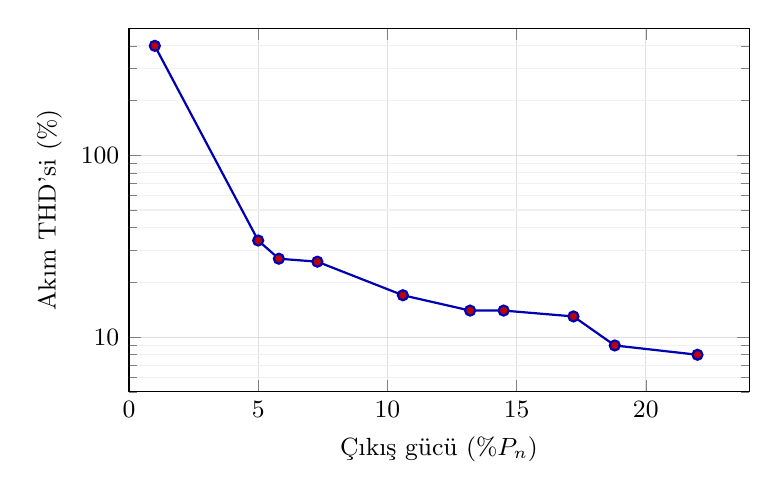
\begin{tikzpicture}
\begin{semilogyaxis}[
  width=0.78\textwidth, height=62mm,
  tick label style={font=\fontsize{9}{10.5}\selectfont}, label style={font=\fontsize{9}{10.5}\selectfont},
  xlabel={Çıkış gücü (\%$P_n$)}, ylabel={Akım THD'si (\%)},
  xmin=0, xmax=24, ymin=5, ymax=500,
  grid=both, grid style={gray!25}, minor grid style={gray!12},
  log basis y=10, log ticks with fixed point, /pgf/number format/use comma,
]
  \addplot[blue!70!black, thick, mark=*, mark size=1.8pt, mark options={fill=red!75!black}] coordinates {
    (1,400) (5,34) (5.8,27) (7.29,26) (10.6,17) (13.2,14) (14.5,14) (17.2,13) (18.8,9) (22,8)};
\end{semilogyaxis}
\end{tikzpicture}

  \caption{Tablo~\ref{tab:ticari-evirici-thd}'deki kaydın grafiği.}
  \label{fig:ticari-evirici-thd}
\end{figure}

Kayıttaki doğrusal olmayan azalma Şekil~\ref{fig:ticari-evirici-thd} üzerinde logaritmik eksende görülmektedir. Akım THD'si anma gücünün \SI{1}{\percent}'inde \SI{400}{\percent} iken \SI{22}{\percent}'sinde \SI{8}{\percent} düzeyine inmektedir. Devreye giriş ve düşük güç test noktaları, anma gücündeki ölçümden ayrı olarak değerlendirilmelidir.

FV profili (Şekil~\ref{fig:fv-calisma-profilleri}, Tablo~\ref{tab:fv-guc-dagilimi}) ile ticari evirici kaydı (Tablo~\ref{tab:ticari-evirici-thd}), düşük güç bölgesinin işletmede sık görüldüğünü ve düşük güçte akım THD'sinin yükseldiğini literatürle birlikte nitel olarak desteklemektedir. Tezdeki verim ve THD bulguları ise deney kayıtlarına ve kalibre edilmiş benzetimlere dayalıdır.

Düşük güçte sürücü, kontrol, anahtarlama ve manyetik elemanların güce zayıf bağlı kayıplarının toplam çıkışa oranı büyümektedir. Şebeke akımının küçük olması, ölü zamanın ve anahtarlama elemanlarının doğrusal olmayan davranışının temel bileşene göre etkisini de artırmaktadır. Saha ve laboratuvar ölçümleri, FV eviricilerde akım dalga biçimi bozulmasının güç seviyesi ve şebeke gerilim kalitesiyle değiştiğini göstermiştir \citep{Kjaer2005,Chicco2009}. Harmonik sınırları bağlantı gücü ve standart kapsamına göre tanımlansa da yalnızca toplam THD değerine bakılması, hangi harmonik bileşenin hangi fiziksel mekanizmadan kaynaklandığını açıklamamaktadır \citep{IEC61000}.

\section{Şebeke Akım Kontrolü ve İleri Besleme Yaklaşımları}

Düşük güç mekanizması tek başına devre düzeyinde çözülemez, çünkü ters akımı kesen her müdahale, akım çevriminin gördüğü denetlenen sistemi de değiştirmektedir. Akım çevriminin temel elemanı olan akım denetleyicisi, şebekeye bağlı bir eviricide referans akım ile ölçülen akım arasındaki hatadan modülasyon gerilimi üretmektedir. Denetleyici yapısı olarak senkron referans çerçevesi, durağan eksen PI kontrolü ve oransal-rezonans (Proportional-Resonant, PR) kontrolü yaygın seçenekler arasındadır. PR denetleyici, temel frekansta yüksek kazanç sağlayarak sinüzoidal referansın kalıcı durum hatasını azaltabilir. Seçili harmoniklerde ek rezonans kolları da kullanılabilir \citep{Teodorescu2006PR,Teodorescu2011}. Akım denetiminin yanında faz kilitlemeli döngü (Phase-Locked Loop, PLL) veya eşdeğer bir eşzamanlama yapısı şebeke faz ve frekans bilgisini üretmekte, tek fazlı sistemlerde ise ortogonal işaret üretimi ve dijital gecikmeler de tasarımın parçası olmaktadır \citep{Blaabjerg2006,Zhou2018}.

LCL filtre, daha küçük toplam endüktansla yüksek frekanslı anahtarlama bileşenlerini zayıflatabilir. Ancak filtre bir rezonans tepesi de oluşturmaktadır. Rezonansı bastırmaya yönelik yöntemlerden pasif sönümleme direnç kaybı doğururken, aktif sönümleme ölçülen akım veya gerilim işaretlerinden sanal empedans etkisi üretmektedir. PR denetleyici ile LCL aktif sönümlemenin birlikte tasarımı, kapalı çevrim kutupları ve kararlılık marjları dikkate alınarak yapılmalıdır \citep{Zhang2014PR}.

Şebeke gerilimi ileri beslemesi ise ortak bağlantı noktasındaki bozucu gerilimin akıma taşınmasını azaltmak için modülasyon girişine ölçülen gerilimden türetilen bir terim eklemektedir. Ancak Lu ve arkadaşları, dijital gecikmenin ileri besleme yolunu LCL rezonansı üzerinde aktif sönümleme veya negatif sönümleme üretebilen dinamik bir elemana dönüştürebildiğini göstermiştir \citep{Lu2016}. Zayıf şebeke koşullarını inceleyen Wang ve arkadaşları da şebeke empedansına bağlı pozitif geri besleme etkisinin faz marjını azaltabileceğini ortaya koymuş ve ileri besleme kanalının frekans seçici biçimde tasarlanması gerektiğini vurgulamıştır \citep{Wang2024}.

Denetleyici ve filtre etkilerinin yanında anahtar ölü zamanı, snubber ve parazitik kapasiteler de komut edilen gerilim ile gerçekleşen faz gerilimi arasında akım yönüne bağlı bir hata oluşturmaktadır. Nitekim Zhang ve Xu, parazitik kapasitelerin anahtarlama kenarlarını sonlu eğimli hâle getirdiğini ve klasik darbe tabanlı ölü zaman kompanzasyonunun özellikle küçük akımlarda yetersiz kalabildiğini deneysel olarak göstermiştir \citep{Zhang2014Deadtime}. Dolayısıyla düşük güç harmonikleri, denetleyici bant genişliğinin yanında modülasyon, anahtar geçişi, akım yönü ve şebeke geriliminin de ortak sonucudur.

Sin\textsuperscript{3} kompanzasyonuna en yakın literatür, kısmi yükte süreksiz iletime giren dönüştürücülerde akım bozulmasının görev oranı kompanzasyonuyla giderilmesidir. Örneğin sürekli iletim için tasarlanan boost PFC dönüştürücüleri düşük yükte şebeke periyodunun bir bölümünde süreksiz iletime girmekte ve klasik akım denetimi giriş akımını bozmaktadır. \citet{DeGusseme2005}, örnek düzeltmesi ile görev oranı ileri beslemesini birleştiren sayısal bir denetimle iki iletim kipinde de düşük harmonikli giriş akımı elde etmiş ve yöntemi \SI{1}{\kilo\watt} prototipte doğrulamıştır. \citet{VanDeSype2005} de görev oranı ileri beslemesinin giriş empedansını dirençsel yaptığını analitik olarak göstermiş ve sıfır geçişi bozulmasını büyük ölçüde gidermiştir. Şebeke eviricisi tarafında ise \citet{Le2019}, sürekli ve süreksiz akım kipinde çalışan tek fazlı bir eviricide süreksiz iletimin yol açtığı doğrusal olmayan davranışı kompanze etmiştir. Bir önceki hesaplama periyodunun görev oranını kullanan kompanzasyon endüktans değerinden bağımsızdır. \SI{4}{\kilo\watt} prototipte daha küçük endüktörle endüktör hacmi \%51 azalmış, 0,1 birim yükteki kayıp ise \%35 düşmüştür. \citet{Wu2013} ise histerezis akım denetimli şebeke eviricisinde sıfır geçişi bozulmasının kaynağını gerçek akım eğiminin referans eğiminden küçük kalmasına bağlamış, kritik faz açısını türetmiş ve çevrimiçi faz öteleme kompanzasyonu önermiştir.

Dört çalışmanın ortak ilkesi, süreksiz iletimin bozduğu akımın görev oranına ya da referansa eklenen bir düzeltme terimiyle giderilmesidir. Tezdeki Sin\textsuperscript{3} terimi ise aynı ilkeyi iki noktada farklı uygulamaktadır. Birincisi, bozulmanın kaynağı diyot doğrultmalı ya da tek anahtarlı bir kat değil, T-tipi nötr kolun bilinçli olarak susturulmasıdır. İkincisi, düzeltme çevrimiçi ölçüm ya da önceki görev oranından değil, şebeke fazından üretilen ve çalışma noktasına kalibre edilen sabit katsayılı bir terimden gelmektedir.

Sin\textsuperscript{3} tabanlı yaklaşımın literatürdeki yerini doğru kurabilmek için üçüncü harmonik enjeksiyonu ile bozucu bastırma amaçlı ileri besleme birbirinden ayrılmalıdır. Klasik üçüncü harmonik enjeksiyonu, faz referanslarına ortak mod bileşeni ekleyerek DA bara kullanım oranını artırmayı veya belirli anahtarlama harmoniklerini düzenlemeyi hedeflemektedir \citep{Holmes2003,Aghdam2013}. Sin\textsuperscript{3} terimi ise nötr anahtar susturma yönteminin oluşturduğu üçüncü harmonik etkisine karşı, ölçülen şebeke işaretinden $\sin^3(\theta)=[3\sin(\theta)-\sin(3\theta)]/4$ özdeşliğiyle üretilen bir şekillendirme bileşenidir. Özdeşliğin Fourier gösterimi terimin matematiksel temelini sağlamaktadır \citep{Oppenheim1997}. Modülasyon girişine eklenen terim, hata sinyalinden türetilen bağımsız bir geri besleme denetleyicisi değil, bir kompanzasyon bileşenidir.

İdeal doğrusal ve doyumsuz modelde dışsal ileri besleme terimi kapalı çevrimin karakteristik paydasını değiştirmeyebilir. Ancak gerçek dönüştürücüde örnekleme, PWM gecikmesi, LCL rezonansı, sınırlayıcılar ve anahtarlamanın çalışma noktasına bağlı doğrusal olmayan davranışı ideal ayrımı sınırlamaktadır. Periyodik çalışma noktaları çevresindeki frekans bağlaşımının incelenmesi gerektiğinde doğrusal zamanla periyodik modeller ve harmonik transfer fonksiyonları (Harmonic Transfer Function, HTF) kullanılabilir \citep{Wereley1991,Liao2022}. Sin\textsuperscript{3} terimi için temel gereksinim, kapalı çevrim aktarımının ve düşük ile anma gücü koşullarındaki etkisinin doğrulanmasıdır.

\section{Literatürün Karşılaştırmalı Değerlendirilmesi}

Makale düzeyindeki çalışmaların yanında konuya yakın doktora tezleri de incelenmiştir. \citet{Kerekes2009}, doktora tezinde transformatörsüz FV eviricilerinde verim kazancının getirdiği kaçak akım sorununu incelemiş ve kaçak akımı standart sınırları içinde tutan topolojileri değerlendirmiştir. \citet{Hartmann2011} ise uçak uygulamaları için üç fazlı PWM doğrultucularda güç yoğunluğu ve verimin birlikte en iyilenmesini ele almış olup çalışması Vienna tipi doğrultucuyu da kapsamaktadır. \citet{Dong2012}, konut ve ticari binalar için DA dağıtım sisteminin merkezindeki çift yönlü AA--DA arayüz dönüştürücüsünü incelemiştir. Dong'un tezinde dengesiz tek fazlı şebeke gücünün DA sistem üzerindeki etkisi çözümlenmiş, iki katlı bir topoloji ve sayısal denetim önerilmiş, ayrıca tam köprüye göre toplam hacmin üç kata kadar azaltılabildiği gösterilmiştir. \citet{Wereley1991} ise doktora tezinde doğrusal zamanla periyodik sistemlerin analizine HTF çerçevesini kazandırmıştır.

Tezdeki üç katkı ekseniyle en yakından ilişkili çalışmalar ise Tablo~\ref{tab:literatur-karsilastirma} üzerinde kullanılan yapı, doğrulama düzeyi, tez açısından kalan sınır ve ilişkili araştırma sorusu bakımından karşılaştırılmıştır. Karşılaştırmanın temel ölçütü, çalışmaların tezdeki araştırma sorularını ne ölçüde kapsadığıdır. Tabloda çalışmalar dört öbekte sıralanmıştır: T-tipi topoloji, hafif yükte süreksiz iletim ve kompanzasyon, akım denetimi ve ileri besleme, işlev paylaşımı ve yeniden yapılandırma.

{\footnotesize
\setlength{\tabcolsep}{3pt}
\begin{longtable}{>{\raggedright\arraybackslash}p{0.18\textwidth} >{\raggedright\arraybackslash}p{0.21\textwidth} >{\raggedright\arraybackslash}p{0.19\textwidth} >{\raggedright\arraybackslash}p{0.28\textwidth} >{\centering\arraybackslash}p{0.05\textwidth}}
\caption{Tezle doğrudan ilişkili çalışmaların karşılaştırmalı sentezi. AS: ilişkili araştırma sorusu.}\label{tab:literatur-karsilastirma}\\
\toprule
\textbf{Çalışma} & \textbf{Yapı ve odak} & \textbf{Doğrulama} & \textbf{Tez açısından kalan sınır} & \textbf{AS} \\
\midrule
\endfirsthead
\caption[]{Tezle doğrudan ilişkili çalışmaların karşılaştırmalı sentezi (devamı).}\\
\toprule
\textbf{Çalışma} & \textbf{Yapı ve odak} & \textbf{Doğrulama} & \textbf{Tez açısından kalan sınır} & \textbf{AS} \\
\midrule
\endhead
\bottomrule
\endfoot
\multicolumn{5}{@{}l}{\textit{T-tipi topoloji}} \\*
\citet{Schweizer2013} & Üç seviyeli T-tipi dönüştürücü (kayıp ve verim) & Analitik kayıp hesabı ve donanım prototipi & Düşük güçte nötr kol ters akımı ve ters akıma bağlı THD ele alınmamıştır. & 1, 2 \\
\citet{Schweizer2013Karsilastirma} & Üç seviyeli topolojilerin iki seviyeli sistemlerle karşılaştırması (çip alanı, harmonik kayıp, pasif hacim) & Karşılaştırmalı analitik değerlendirme & Ölçüt tasarım noktasıdır. Düşük akımda nötr kol akım yolu karşılaştırılmamıştır. & 1 \\
\citet{Wang2020} & \SI{250}{\kilo\watt} SiC T-tipi evirici (güç yoğunluğu ve geçiş kayıpları) & Kayıp modeli ve tam ölçekli prototip & Çalışma çekiş eviricisine ve yüksek güç tasarımına odaklanmıştır. & 1 \\
\citet{Kerekes2009} (doktora tezi) & Transformatörsüz FV eviricileri (kaçak akım ve topoloji seçimi) & Analiz ve modelleme & Verim--kaçak akım ödünleşimi incelenmiştir. Düşük güç verim--THD ödünleşimi kapsam dışıdır. & 2 \\
\midrule
\multicolumn{5}{@{}l}{\textit{Hafif yükte süreksiz iletim ve kompanzasyon}} \\*
\citet{Chen2010} & Senkron alçaltıcı (diyot benzetimi ve sürekli iletim) & Analiz, benzetim ve deney & T-tipi şebeke eviricisinin sıfır durumu ve harmonik sonucu kapsanmamıştır. & 1, 2 \\
\citet{DeGusseme2005} & Boost PFC (sürekli ve süreksiz iletimde sayısal denetim, görev oranı ileri beslemesi) & \SI{1}{\kilo\watt} prototip & Bozulma kaynağı tek anahtarlı PFC katıdır. Şebeke eviricisi ve kararlılık etkisi ele alınmamıştır. & 3 \\
\citet{VanDeSype2005} & Boost PFC (görev oranı ileri beslemesi, giriş empedansı) & Analitik model ve prototip & Sıfır geçişi bozulması hedeflenmiştir. Üçüncü harmonik ağırlıklı alternans içi bozulma kapsanmamıştır. & 3 \\
\citet{Le2019} & Tek fazlı şebeke eviricisi (iki akım kipinde, endüktanstan bağımsız süreksiz iletim kompanzasyonu) & \SI{4}{\kilo\watt}, \SI{100}{\kilo\hertz} prototip & Süreksiz iletim küçük endüktör tasarımından gelmektedir. Nötr anahtar susturma ve T-tipi yapı ele alınmamıştır. & 2, 3 \\
\citet{Wu2013} & Histerezis akım denetiminde sıfır geçişi bozulması & Analiz, benzetim ve deney & Kompanzasyon faz ötelemedir. Anahtarlama kipinin değiştirilmesinden doğan bozulma kapsanmamıştır. & 3 \\
\citet{Zhang2014Deadtime} & Ölü zaman ve parazitik kapasite kompanzasyonu & Darbe modeli ve deney & Nötr anahtar susturma kaynaklı üçüncü harmonik hedeflenmemiştir. & 3 \\
\midrule
\multicolumn{5}{@{}l}{\textit{Akım denetimi ve ileri besleme}} \\*
\citet{Lu2016} & LCL eviricide şebeke gerilimi ileri beslemesi & Frekans alanı analizi ve deney & Sin\textsuperscript{3} tabanlı anlık şekillendirme ve düşük güç ters akımı ele alınmamıştır. & 3 \\
\citet{Wang2024} & Zayıf şebekede filtreli ileri besleme & Empedans modeli ve yarı fiziksel benzetim & Amaç anahtarlama kaynaklı üçüncü harmonik değil, şebeke empedansına uyumdur. & 3 \\
\citet{Dong2012} (doktora tezi) & Çift yönlü tek fazlı AA--DA arayüz dönüştürücüsü (DA dağıtım sistemi) & Analiz, topoloji ve sayısal denetim tasarımı & İki katlı topoloji ve sistem düzeyi denetim incelenmiştir. T-tipi düşük güç anahtarlaması kapsam dışıdır. & 3, 4 \\
\midrule
\multicolumn{5}{@{}l}{\textit{İşlev paylaşımı ve yeniden yapılandırma}} \\*
\citet{Haghbin2013} & Araçta tümleşik şarj (sürücü elemanlarının şarjda kullanımı) & İnceleme ve önerilen yalıtımlı şarj devresi & Çekiş sürücüsü ve motor sargısı üzerine kuruludur. Sabit EDS'de T-tipi ve Vienna işlev paylaşımı ele alınmamıştır. & 4 \\
\citet{Yilmaz2013} & Şarj cihazı topolojileri, güç seviyeleri ve altyapı & İnceleme & Sınıflandırma çalışmasıdır. Ortak yarı iletken tabanlı kip geçişi ayrıntılandırılmamıştır. & 4 \\
\citet{Hartmann2011} (doktora tezi) & Üç fazlı PWM ve Vienna tipi doğrultucular (güç yoğunluğu ve verim) & Karşılaştırmalı tasarım ve en iyileme & Doğrultucu tek işlevlidir. Evirici ve batarya yönetimiyle donanım paylaşımı ele alınmamıştır. & 4 \\
\citet{Momayyezan2016} & Yeniden yapılandırılabilir yüksek gerilim batarya dönüştürücüsü & Beş modüllü ölçekli prototip & Şebekeye bağlı üç seviyeli T-tipi evirici ve düşük güç yöntemiyle bütünleşmemiştir. & 4 \\
\citet{Farakhor2023} & Modüler yeniden yapılandırılabilir BESS ve hücre gücü yönetimi & Optimizasyon, benzetim ve laboratuvar prototipi & T-tipi/Vienna işlev paylaşımı ve şebeke akımı kalitesi hedeflenmemiştir. & 4 \\
\citet{Huang2024} & Anahtar tabanlı modüler yeniden yapılandırma ve dengeleme & Kayıp analizi ve ölçekli deney & İlave modül anahtarları kullanılmıştır. Ortak T-tipi güç katı ele alınmamıştır. & 4 \\
\end{longtable}
}


\section{Araştırma Boşluğu}

Literatür taraması dört ayrı bilgi kümesinin gelişmiş olduğunu göstermiştir. T-tipi dönüştürücüye ilişkin çalışmalar yüksek verim, güç yoğunluğu, anahtarlama geçişleri ve elektromanyetik uyumluluk özelliklerini anma ve tasarım noktasında açıklamaktadır \citep{Schweizer2013,Schweizer2013Karsilastirma,Wang2020,Hizarci2021}. Hafif yük çalışmaları ise ters akımı azaltan süreksiz iletim veya diyot benzetimi ilkelerini ve süreksiz iletimin bozduğu akımın görev oranı ileri beslemesiyle düzeltilmesini incelemektedir \citep{Chen2010,DeGusseme2005,VanDeSype2005,Le2019,Wu2013}. Şebeke eviricilerinde akım denetimi, LCL kararlılığı ve şebeke gerilimi ileri beslemesi de ayrı bir literatür oluşturmaktadır \citep{Lu2016,Wang2024,Zhang2014PR}. Son olarak işlev paylaşımı çalışmaları, eviricinin yarı iletkenlerini şarj kipinde yeniden kullanan tümleşik şarj cihazlarını ve batarya modüllerini farklı çalışma kiplerinde yeniden kullanan EDS mimarilerini geliştirmektedir \citep{Haghbin2013,Yilmaz2013,Momayyezan2016,Farakhor2023,Huang2024}.

Ne var ki kümeler arasındaki bağlantı sınırlıdır. Birincisi, T-tipi eviricinin düşük güçte sıfır durumunu oluşturan nötr kolun senkron alçaltıcı benzeri ters akım mekanizması, aynı müdahalenin verim ve üçüncü harmonik üzerindeki karşıt etkileriyle birlikte yeterince incelenmemiştir. İkincisi, süreksiz iletim bozulmasının kompanzasyonu PFC katları ve küçük endüktörlü şebeke eviricileri için çevrimiçi yöntemlerle geliştirilmiş olsa da T-tipi yapıda bozulma nötr anahtarın bilinçli susturulmasından doğmaktadır. Dolayısıyla şebeke fazından üretilen sabit katsayılı bir Sin\textsuperscript{3} teriminin bozulmayı ne ölçüde giderdiği ve akım çevriminin kararlılığını değiştirip değiştirmediği açık bir sorudur. Üçüncüsü, tümleşik şarj ve yeniden yapılandırılabilir batarya literatüründe işlev paylaşımının mümkün olduğu görülmekle birlikte, T-tipi evirici, Vienna PFC ve aktif batarya yönetimi işlevlerinin aynı yarı iletken yapıda birleştirilmesi düşük güç anahtarlama ve şebeke akımı kalitesi ekseniyle ortak bir tez çerçevesinde incelenmemiştir.

Belirlenen araştırma boşluğu, üç katkıyı tek bir sav altında birleştirmektedir. Sav, T-tipi dönüştürücünün anahtarlama durumlarının düşük güçte ters akımı azaltacak biçimde yeniden düzenlenebileceğini, ortaya çıkan harmonik ödünleşiminin Sin\textsuperscript{3} tabanlı ileri besleme kompanzasyonuyla yönetilebileceğini ve aynı topolojinin yarı iletkenlerinin EDS'nin farklı şarj--deşarj ve dengeleme kiplerinde yeniden görevlendirilebileceğini önermektedir.

\chapter{SİSTEM MİMARİSİ, MODEL VE METODOLOJİ}
\label{chap:sistem}
% T-tipi faz kolu için ortak vektör çizim tabanı.
% Argümanlar: Q1, Q2, orta nokta tarafı nötr anahtar (Q4, düğüm q3), faz tarafı nötr anahtar (Q3, düğüm q4) çizgi renkleri ve ek TikZ yolu.
% Adlandırma (09.11.2026, K-31): tümleyen çiftler Q1--Q3 ve Q2--Q4; düğüm adları konumu gösterir.
\newcommand{\ttypevector}[5]{%
\begin{tikzpicture}[
  x=0.76cm,y=0.56cm,
  terminal/.style={circle,fill=black,inner sep=1.25pt},
  sw/.style={rounded corners=1pt,minimum width=7mm,minimum height=8mm,fill=white,font=\scriptsize},
  bus/.style={line width=0.8pt},
  current/.style={-{Latex[length=2mm]},red!80!black,line width=1.7pt},
  activepath/.style={blue!70!black,line width=2.0pt}
]
  % Bölünmüş DA bara ve kapasitörler
  \draw[bus] (0,5) -- (4,5);
  \draw[bus] (0,-1) -- (4,-1);
  \draw[bus] (0,5) -- (0,3.65);
  \draw[bus] (-0.32,3.65) -- (0.32,3.65);
  \draw[bus] (-0.32,3.35) -- (0.32,3.35);
  \draw[bus] (0,3.35) -- (0,2);
  \draw[bus] (0,2) -- (0,0.65);
  \draw[bus] (-0.32,0.65) -- (0.32,0.65);
  \draw[bus] (-0.32,0.35) -- (0.32,0.35);
  \draw[bus] (0,0.35) -- (0,-1);
  \node[font=\scriptsize,left] at (0,5) {$+V_{\mathrm{dc}}/2$};
  \node[font=\scriptsize,left] at (0,2) {$N$};
  \node[font=\scriptsize,left] at (0,-1) {$-V_{\mathrm{dc}}/2$};
  \node[font=\scriptsize,left] at (-0.38,3.5) {$C_A$};
  \node[font=\scriptsize,left] at (-0.38,0.5) {$C_B$};

  % Ana anahtarlar ve çift yönlü nötr kol
  \node[sw,draw=#1,line width=1.25pt] (q1) at (4,3.65) {$Q_1$};
  \node[sw,draw=#2,line width=1.25pt] (q2) at (4,0.35) {$Q_2$};
  \node[sw,draw=#3,line width=1.25pt] (q3) at (1.55,2) {$Q_4$};
  \node[sw,draw=#4,line width=1.25pt] (q4) at (2.75,2) {$Q_3$};
  \draw[bus] (4,5) -- (q1.north);
  \draw[bus] (q1.south) -- (4,2);
  \draw[bus] (4,2) -- (q2.north);
  \draw[bus] (q2.south) -- (4,-1);
  \draw[bus] (0,2) -- (q3.west);
  \draw[bus] (q3.east) -- (q4.west);
  \draw[bus] (q4.east) -- (5.15,2);
  \node[terminal] at (0,2) {};
  \node[terminal] (out) at (4,2) {};
  \draw[-{Latex[length=1.8mm]},thick] (out) -- (5.15,2);
  \node[font=\scriptsize,right] at (5.15,2) {$v_{xN},\ i_x$};
  #5
\end{tikzpicture}%
}

% Faz başına tam T-tipi güç devresi: bölünmüş DA bara, dört IGBT ve LCL filtre.
% Filtre kapasitörü modelle tutarlı olarak C_f adıyla gösterilir.
\newcommand{\ttypefulltopology}{%
\begin{tikzpicture}[
  x=0.88cm,y=0.68cm,
  wire/.style={line width=0.9pt},
  coilpath/.style={decorate,decoration={coil,aspect=0.48,segment length=2.8mm,amplitude=1.8mm}},
  igbt/.style={nigbt,bodydiode,anchor=C,tr circle=false},
  terminal/.style={circle,fill=black,inner sep=1.35pt},
  label/.style={font=\scriptsize,align=center}
]
  \ctikzset{transistors/scale=0.85,transistor bodydiode/scale=0.40}
  % Bölünmüş DA bara ve orta nokta
  \draw[wire] (0,5) -- (5.3,5);
  \draw[wire] (0,-1) -- (5.3,-1);
  \draw[wire] (0,5) -- (0,3.65);
  \draw[wire] (-0.38,3.65) -- (0.38,3.65);
  \draw[wire] (-0.38,3.35) -- (0.38,3.35);
  \draw[wire] (0,3.35) -- (0,2);
  \draw[wire] (0,2) -- (0,0.65);
  \draw[wire] (-0.38,0.65) -- (0.38,0.65);
  \draw[wire] (-0.38,0.35) -- (0.38,0.35);
  \draw[wire] (0,0.35) -- (0,-1);
  \node[label,left] at (0,5) {$\mathrm{DC}^{+}$};
  \node[label,above left=0.7mm and 0.8mm] at (0,2) {$N$};
  \node[label,left] at (0,-1) {$\mathrm{DC}^{-}$};
  \node[label,left=1mm] at (-0.38,3.50) {$C_A$};
  \node[label,left=1mm] at (-0.38,0.50) {$C_B$};
  \node[terminal] at (0,2) {};

  % Dış faz kolu ve emetörden kolektöre yönelen antiparalel diyotlar.
  \node[igbt] (q1) at (5.3,4.43) {};
  \node[igbt] (q2) at (5.3,1.13) {};
  \draw[wire] (5.3,5) -- (q1.C);
  \draw[wire] (q1.E) -- (5.3,2);
  \draw[wire] (5.3,2) -- (q2.C);
  \draw[wire] (q2.E) -- (5.3,-1);
  \node[label,right] at (6.15,3.94) {$Q_1$};
  \node[label,right] at (6.15,3.44) {$DS_1$};
  \node[label,right] at (6.15,0.64) {$Q_2$};
  \node[label,right] at (6.15,0.14) {$DS_2$};
  \node[terminal] (pole) at (5.3,2) {};

  % Nötr kol: Q4 ve Q3'ün emetörleri ortada birleşir.
  \node[igbt,rotate=90] (q4) at (1.02,2) {};
  \node[igbt,rotate=-90,xscale=-1] (q3) at (4.40,2) {};
  \draw[wire] (0,2) -- (q4.C);
  \draw[wire] (q4.E) -- (q3.E);
  \draw[wire] (q3.C) -- (pole);
  \node[label,below] at (1.65,0.98) {$Q_4$};
  \node[label,below] at (3.78,0.98) {$Q_3$};
  \node[label,above] at (1.65,2.77) {$DS_4$};
  \node[label,above] at (3.78,2.77) {$DS_3$};

  % Faz başına LCL filtre ve şebeke/yük terminali
  \coordinate (l1a) at (6.35,2);
  \coordinate (l1b) at (7.45,2);
  \coordinate (cnode) at (8.15,2);
  \coordinate (l2a) at (8.85,2);
  \coordinate (l2b) at (9.95,2);
  \draw[wire] (pole) -- (l1a);
  \draw[coilpath,line width=0.9pt] (l1a) -- (l1b);
  \draw[wire] (l1b) -- (cnode) -- (l2a);
  \draw[coilpath,line width=0.9pt] (l2a) -- (l2b);
  \draw[wire,-{Latex[length=1.8mm]}] (l2b) -- (11.1,2);
  \node[label,above=1.5mm] at ($(l1a)!0.5!(l1b)$) {$L_1$};
  \node[label,above=1.5mm] at ($(l2a)!0.5!(l2b)$) {$L_2$};
  \node[label,right] at (11.1,2) {$v_g,\ i_2$};
  \node[terminal] at (cnode) {};
  \draw[wire] (cnode) -- (8.15,1.25);
  \draw[wire] (7.78,1.25) -- (8.52,1.25);
  \draw[wire] (7.78,0.95) -- (8.52,0.95);
  \draw[wire] (8.15,0.95) -- (8.15,-1.45) -- (-1.20,-1.45);
  \draw[wire] (-1.20,-1.45) -- (-1.20,2) -- (0,2);
  \node[label,right=1mm] at (8.52,1.10) {$C_f$};
  \draw[-{Latex[length=1.8mm]},red!80!black,line width=1.1pt] (6.0,2.30) -- (7.0,2.30);
  \node[label,above] at (6.5,2.30) {$i_1$};
\end{tikzpicture}%
}

% Senkron-buck eşdeğeri: üst ray, alt ray, üst ve alt anahtar etiketleri,
% enerji aktaran anahtarın konumu (1: üst, 0: alt). Yeşil anahtar ve mavi yol aktif enerji aktarımıdır (K-32).
\newcommand{\syncbuckvector}[5]{%
\begin{tikzpicture}[
  x=0.82cm,y=0.65cm,
  sw/.style={draw,rounded corners=1pt,minimum width=8mm,minimum height=8mm,fill=white,font=\scriptsize},
  coilpath/.style={decorate,decoration={coil,aspect=0.48,segment length=2.7mm,amplitude=1.8mm}},
  current/.style={-{Latex[length=2mm]},red!80!black,line width=1.4pt}
]
  \draw[line width=0.8pt] (0,3.2) -- (1.8,3.2);
  \draw[line width=0.8pt] (0,0) -- (1.8,0);
  \node[font=\scriptsize,left] at (0,3.2) {#1};
  \node[font=\scriptsize,left] at (0,0) {#2};
  \ifnum#5=1
    \node[sw,draw=green!55!black,line width=1.2pt] (qh) at (1.8,2.45) {#3};
    \node[sw,draw=gray!65,line width=1.2pt] (ql) at (1.8,0.75) {#4};
  \else
    \node[sw,draw=gray!65,line width=1.2pt] (qh) at (1.8,2.45) {#3};
    \node[sw,draw=green!55!black,line width=1.2pt] (ql) at (1.8,0.75) {#4};
  \fi
  \draw[line width=0.8pt] (1.8,3.2) -- (qh.north);
  \draw[line width=0.8pt] (qh.south) -- (1.8,1.6);
  \draw[line width=0.8pt] (1.8,1.6) -- (ql.north);
  \draw[line width=0.8pt] (ql.south) -- (1.8,0);
  \fill (1.8,1.6) circle (1.5pt);
  \coordinate (l1a) at (2.45,1.6);
  \coordinate (l1b) at (3.35,1.6);
  \coordinate (cnode) at (3.88,1.6);
  \coordinate (l2a) at (4.30,1.6);
  \coordinate (l2b) at (5.20,1.6);
  \draw[line width=0.8pt] (1.8,1.6) -- (l1a);
  \draw[coilpath,line width=0.9pt] (l1a) -- (l1b);
  \draw[line width=0.8pt] (l1b) -- (cnode) -- (l2a);
  \draw[coilpath,line width=0.9pt] (l2a) -- (l2b);
  \ifnum#5=1
    \draw[current] (l2b) -- (6.0,1.6);
  \else
    \draw[current] (6.0,1.6) -- (l2b);
  \fi
  \node[font=\scriptsize,above=2mm] at ($(l1a)!0.5!(l1b)$) {$L_1$};
  \node[font=\scriptsize,above=2mm] at ($(l2a)!0.5!(l2b)$) {$L_2$};
  \node[font=\scriptsize,right] at (6.0,1.6) {$v_g,\ i_L$};
  \fill (cnode) circle (1.3pt);
  \draw[line width=0.8pt] (cnode) -- (3.88,1.0);
  \draw[line width=0.8pt] (3.55,1.0) -- (4.21,1.0);
  \draw[line width=0.8pt] (3.55,0.75) -- (4.21,0.75);
  \draw[line width=0.8pt] (3.88,0.75) -- (3.88,0.2);
  \draw[line width=0.8pt] (3.58,0.2) -- (4.18,0.2);
  \draw[line width=0.8pt] (3.68,0.05) -- (4.08,0.05);
  \node[font=\scriptsize,right] at (4.18,0.88) {$C_f$};
  \ifnum#5=1
    \draw[blue!70!black,line width=1.8pt] (0.5,3.2) -| (qh.north);
    \draw[blue!70!black,line width=1.8pt] (qh.south) -- (1.8,1.6) -- (l1a);
  \else
    \draw[blue!70!black,line width=1.8pt] (l1a) -- (1.8,1.6) -- (ql.north);
    \draw[blue!70!black,line width=1.8pt] (ql.south) -- (1.8,0) -- (0.5,0);
  \fi
\end{tikzpicture}%
}

% Susturmalı yarım periyot eşdeğeri: bir aktif anahtar ve tek yönlü serbest dolaşım yolu.
% Argümanlar: üst ray, alt ray, aktif anahtar, diyot etiketi, anahtar konumu (1: üst, 0: alt).
% Diyot her iki yarım periyotta yukarı yönlüdür: pozitifte N'den kutba, negatifte kutuptan N'ye.
\newcommand{\susturmabuckvector}[5]{%
\begin{tikzpicture}[
  x=0.82cm,y=0.65cm,
  sw/.style={draw,rounded corners=1pt,minimum width=8mm,minimum height=8mm,fill=white,font=\scriptsize},
  coilpath/.style={decorate,decoration={coil,aspect=0.48,segment length=2.7mm,amplitude=1.8mm}},
  current/.style={-{Latex[length=2mm]},red!80!black,line width=1.4pt},
  freewheel/.style={orange!85!black,line width=1.6pt,dash pattern=on 3pt off 1.6pt}
]
  \draw[line width=0.8pt] (0,3.2) -- (1.8,3.2);
  \draw[line width=0.8pt] (0,0) -- (1.8,0);
  \node[font=\scriptsize,left] at (0,3.2) {#1};
  \node[font=\scriptsize,left] at (0,0) {#2};
  \fill (1.8,1.6) circle (1.5pt);
  \ifnum#5=1
    \node[sw,draw=green!55!black,line width=1.2pt] (q) at (1.8,2.45) {#3};
    \draw[line width=0.8pt] (1.8,3.2) -- (q.north);
    \draw[line width=0.8pt] (q.south) -- (1.8,1.6);
    \coordinate (da) at (1.8,0.52); \coordinate (dk) at (1.8,1.08);
    \draw[line width=0.8pt] (1.8,0) -- (da); \draw[line width=0.8pt] (dk) -- (1.8,1.6);
  \else
    \node[sw,draw=green!55!black,line width=1.2pt] (q) at (1.8,0.75) {#3};
    \draw[line width=0.8pt] (1.8,1.6) -- (q.north);
    \draw[line width=0.8pt] (q.south) -- (1.8,0);
    \coordinate (da) at (1.8,2.12); \coordinate (dk) at (1.8,2.68);
    \draw[line width=0.8pt] (1.8,1.6) -- (da); \draw[line width=0.8pt] (dk) -- (1.8,3.2);
  \fi
  % diyot: anot (da) altta, katot (dk) üstte
  \filldraw[fill=white,draw=orange!85!black,line width=1.1pt] ($(da)+(-0.24,0)$) -- ($(da)+(0.24,0)$) -- (dk) -- cycle;
  \draw[orange!85!black,line width=1.3pt] ($(dk)+(-0.24,0)$) -- ($(dk)+(0.24,0)$);
  \node[font=\scriptsize,left=1.2mm,align=right] at ($(da)!0.5!(dk)+(-0.24,0)$) {#4};
  \coordinate (l1a) at (2.45,1.6);
  \coordinate (l1b) at (3.35,1.6);
  \coordinate (cnode) at (3.88,1.6);
  \coordinate (l2a) at (4.30,1.6);
  \coordinate (l2b) at (5.20,1.6);
  \draw[line width=0.8pt] (1.8,1.6) -- (l1a);
  \draw[coilpath,line width=0.9pt] (l1a) -- (l1b);
  \draw[line width=0.8pt] (l1b) -- (cnode) -- (l2a);
  \draw[coilpath,line width=0.9pt] (l2a) -- (l2b);
  \node[font=\scriptsize,above=2mm] at ($(l1a)!0.5!(l1b)$) {$L_1$};
  \node[font=\scriptsize,above=2mm] at ($(l2a)!0.5!(l2b)$) {$L_2$};
  \fill (cnode) circle (1.3pt);
  \draw[line width=0.8pt] (cnode) -- (3.88,1.0);
  \draw[line width=0.8pt] (3.55,1.0) -- (4.21,1.0);
  \draw[line width=0.8pt] (3.55,0.75) -- (4.21,0.75);
  \draw[line width=0.8pt] (3.88,0.75) -- (3.88,0.2);
  \draw[line width=0.8pt] (3.58,0.2) -- (4.18,0.2);
  \draw[line width=0.8pt] (3.68,0.05) -- (4.08,0.05);
  \node[font=\scriptsize,right] at (4.18,0.88) {$C_f$};
  \ifnum#5=1
    \draw[current] (l2b) -- (6.0,1.6);
    \draw[blue!70!black,line width=1.8pt] (0.5,3.2) -| (q.north);
    \draw[blue!70!black,line width=1.8pt] (q.south) -- (1.8,1.6) -- (l1a);
    \draw[freewheel] (0.5,0) -- (1.8,0) -- (da);
    \draw[freewheel] (dk) -- (1.8,1.6);
  \else
    \draw[current] (6.0,1.6) -- (l2b);
    \draw[blue!70!black,line width=1.8pt] (l1a) -- (1.8,1.6) -- (q.north);
    \draw[blue!70!black,line width=1.8pt] (q.south) -- (1.8,0) -- (0.5,0);
    \draw[freewheel] (1.8,1.6) -- (da);
    \draw[freewheel] (dk) -- (1.8,3.2) -- (0.5,3.2);
  \fi
  \node[font=\scriptsize,right] at (6.0,1.6) {$v_g,\ i_L$};
\end{tikzpicture}%
}


Literatür incelemesi, T-tipi dönüştürücünün yüksek verim ve güç yoğunluğu bakımından güçlü bir seçenek olduğunu göstermiştir. Aynı inceleme, hafif yükteki ters akımın, nötr kol kullanımının ve şebeke akımı harmoniklerinin aynı sistem sınırı içinde ele alınması gerektiğini de ortaya koymuştur. Tezde incelenen yapı, bölünmüş doğru akım (DA) bara, T-tipi güç katı, LCL çıkış filtresi, şebeke bağlantısı, ölçüm zinciri ve sayısal denetim biriminden oluşmaktadır. Kapsam iki düzeyde ayrılmaktadır. Laboratuvar prototipi üç fazlı, dört telli bir güç katıdır ve nötr hattı DA bara orta noktasına bağlıdır. Benzetim modelleri ile laboratuvar deneyleri ise prototipin tek faz kolunu kapsamaktadır. Şebeke dönüş akımı DA bara orta noktasına girmektedir. Bütün güç, akım ve verim değerleri faz başına verilmiştir. Deneyler güvenli laboratuvar koşulunda, varyak üzerinden yaklaşık \SI{120}{\volt} şebeke geriliminde ve yaklaşık \SI{2.3}{\ampere} faz akımında yürütülmüştür. Bölümün ilk amacı, önerilen yöntemlerin uygulanacağı fiziksel sistemi tanımlamak ve anahtarlama durumlarını ortak bir gösterim altında toplamaktır. Bölüm ayrıca sonraki analizlerin dayanacağı matematiksel modeli kurmakta ve benzetim modelinin tez tanımına göre nasıl doğrulandığını belgelemektedir.

Model, ideal anahtarlama durumlarını açıklayan devre düzeyini, LCL filtre ile denetim çevrimini açıklayan ortalama değer düzeyinden ayırmaktadır. Topolojiye ilişkin iddialar çok seviyeli dönüştürücü ve hafif yük literatürüyle sınanmıştır \citep{Mohan2003,Holmes2003,Schweizer2013,Wang2020,Chen2010}. Yarı iletken gerilim düşümleri, ters toparlanma, ölü zaman ve modülasyon doygunluğu anahtarlamalı benzetim katmanında ele alınmaktadır. Örnekleme gecikmesi ise kararlılık analizinde ayrıca ele alınmıştır.

\section{Sistemin Genel Mimarisi ve İnceleme Sınırı}

Şekil~\ref{fig:genel-sistem-mimarisi}, enerji, ölçüm ve denetim yollarını aynı çerçevede göstermektedir. Deşarj yönünde enerjinin kaynağı batarya veya ayarlanabilir DA kaynaktır. Enerji, bölünmüş DA bara üzerinden T-tipi güç katına aktarılmakta ve anahtarlanan faz gerilimleri LCL filtre aracılığıyla şebeke akımına dönüştürülmektedir. Akım ve gerilim ölçümleri sayısal denetim birimine taşınmakta, üretilen modülasyon komutları kapı sürücüleri üzerinden güç katına uygulanmaktadır. Sin\textsuperscript{3} kompanzasyonunun hedefi, nötr anahtar susturma yönteminin düşük güçte oluşturduğu üçüncü harmonik bileşendir.

\begin{figure}[H]
  \centering
  \resizebox{0.98\textwidth}{!}{%
  \begin{tikzpicture}[
    node distance=8mm and 8mm,
    block/.style={draw, rounded corners=1.5pt, align=center, minimum height=11mm, minimum width=24mm, fill=blue!5},
    ctrl/.style={draw, rounded corners=1.5pt, align=center, minimum height=10mm, minimum width=25mm, fill=orange!10},
    meas/.style={draw, rounded corners=1.5pt, align=center, minimum height=9mm, minimum width=24mm, fill=gray!10},
    flow/.style={-{Latex[length=2mm]}, thick},
    sig/.style={-{Latex[length=2mm]}, thick, dashed}
  ]
    \node[block] (bat) {Batarya /\\DA kaynak};
    \node[block, right=of bat] (dc) {Bölünmüş\\DA bara};
    \node[block, right=of dc] (inv) {T-tipi\\güç katı};
    \node[block, right=of inv] (lcl) {LCL\\filtre};
    \node[block, right=of lcl] (grid) {Şebeke /\\ortak bağlantı};
    \draw[flow] (bat) -- node[above, font=\scriptsize]{enerji} (dc);
    \draw[flow] (dc) -- (inv);
    \draw[flow] (inv) -- (lcl);
    \draw[flow] (lcl) -- (grid);

    \node[meas, below=15mm of lcl] (meas) {Gerilim ve akım\\ölçümleri};
    \node[ctrl, left=of meas] (pwm) {PWM ve kapı\\sinyalleri};
    \node[ctrl, left=of pwm] (control) {Akım denetimi ve\\sınırlandırıcılar};
    \node[ctrl, below=of control] (sin3) {{Sin\textsuperscript{3}}\\kompanzasyonu};
    \draw[sig] (grid.south) |- (meas.east);
    \draw[sig] (lcl.south) -- (meas.north);
    \draw[sig] (meas) -- (control);
    \draw[sig] (control) -- (pwm);
    \draw[sig] (sin3) -- (control);
    \draw[sig] (pwm.north) |- (inv.south);
  \end{tikzpicture}%
  }
  \caption{Genel sistem mimarisi: güç yolu, geri besleme yolu ve Sin\textsuperscript{3} kompanzasyonu.}
  \label{fig:genel-sistem-mimarisi}
\end{figure}

İnceleme sınırı üç katman üzerinden kurulmuştur. Fiziksel katman yarı iletkenleri, bölünmüş DA barayı, filtreyi ve şebeke bağlantısını kapsamaktadır. Denetim katmanı ölçüm, akım regülasyonu, modülasyon ve kapı sinyali üretimini içermektedir. Doğrulama katmanının kapsamı ise benzetim ile deneyde ortak kullanılan çalışma noktaları ve performans ölçütleridir. GT-tipi yeniden yapılandırma, aynı yarı iletkenlerin şarj ve deşarj kiplerinde farklı görevlerde kullanılmasına dayanmaktadır. Ayrıntılı işlev paylaşımı Bölüm~\ref{chap:gttipi} altında ele alınmıştır. Bölüm, deşarj yönündeki T-tipi evirici davranışını ve önerilen düşük güç yöntemlerinin dayandığı modeli sabitlemektedir.

Her iddia, kendisini en doğrudan sınayan model katmanıyla desteklenmiştir. Tablo~\ref{tab:model-katmanlari}, bölümde kullanılan model katmanlarını, her katmanın kapsadığı etkileri, sınadığı konuyu ve tamamlayıcı katmanını birlikte vermektedir. Katman ayrımı, ortalama değerli denetim modelinden elde edilen kararlılık sonucunu anahtarlama kaybı ve deneysel verim kanıtından ayrı tutmaktadır.

\begin{table}[H]
  \centering
  \caption{Model ve doğrulama katmanlarının amacı, sınadığı konu ve tamamlayıcı katmanı.}
  \label{tab:model-katmanlari}
  \small
  \begin{tabularx}{\textwidth}{p{0.21\textwidth} p{0.27\textwidth} X X}
    \toprule
    Katman & Temel içerik & Sınanan konu & Tamamlayıcı katman ve konu \\
    \midrule
    İdeal anahtarlama durumu & $P$--$O$--$N$ seviyeleri ve akım yönü & Geçerli kapı durumu, gerilim seviyesi ve iletim yolu & Anahtarlamalı benzetim: ölü zaman, kayıp ve THD \\
    Ortalama LCL/denetim modeli & $L_1$--$C_f$--$L_2$, gecikme ve $C_i(s)$ & Akım izleme, kutuplar ve kararlılık marjı & Anahtarlamalı benzetim: yarı iletken geçiş kaybı \\
    Anahtarlamalı benzetim & Gerçek PWM, kapı mantığı ve ideal olmayan elemanlar & Ters akım, harmonikler, anahtarlama sayısı ve geçici rejim & Deneysel sistem: donanımda ölçülen verim ve THD \\
    Deneysel sistem & Güç katı, sensör, sürücü, ADC ve gerçek zamanlı kod & Verim, THD, koruma ve uygulanabilirlik & S4 benzetimi: orta ve anma akımı bölgesi \\
    \bottomrule
  \end{tabularx}
\end{table}

\section{T-Tipi Faz Kolu ve Anahtarlama Durumları}

Faz kolunun devre yapısı ve $Q_1$--$Q_4$ adlandırması Şekil~\ref{fig:t-tipi-faz-kolu} üzerinde verilmiştir. $Q_1$--$Q_4$, Tablo~\ref{tab:sistem-parametreleri} içindeki $S_1$--$S_4$ anahtarlarıyla birebir aynıdır. Bölünmüş bara geriliminin toplamı $V_{\mathrm{dc}}$ kabul edildiğinde ideal faz-kutup gerilimi $+V_{\mathrm{dc}}/2$, $0$ ve $-V_{\mathrm{dc}}/2$ seviyelerinden birini almaktadır. Nötr kolun eklediği sıfır seviyesi, iki seviyeli yapıya göre daha küçük gerilim basamakları oluşturmaktadır. Karşılığında komütasyon düzeninin ve nötr nokta akımının ayrıca yönetilmesi gerekmektedir \citep{Schweizer2013,Wang2020}.

Sistemin tam açık güç şeması Şekil~\ref{fig:gelen-tam-topoloji} üzerinde, birinci faz hücresi ise okunabilir ölçekte Şekil~\ref{fig:gelen-faz1-hucresi} üzerinde verilmiştir. Sistem sınırı şemaya göre belirlenmiştir. Şemanın solunda dört iletkenli giriş, ortak-mod endüktansları ve şönt kapasitörlerden oluşan giriş/EMI ağı yer almaktadır. Ortada, ortak DA bağlantısına bağlanan üç tekrarlı T-tipi faz hücresi bulunmaktadır. Her hücrede dış kol anahtar modülü, çift yönlü nötr kol, PFC yükseltici (boost) diyotları, yerel kapasitörler, akım algılama elemanı ve röle vardır. Hücrelerin altındaki nötr hattı, üç fazın DA bara orta noktalarını birbirine ve giriş nötrüne bağlamaktadır. Şemanın en alt kısmında ise GT-tipi mimarinin şarj yönünde kullanılan batarya yönetim sistemi (BYS) transformatörleri görülmektedir. Deney düzeneği GT-tipi mimariye göre kurulmuştur. Her hücredeki röle ($RL1$) ile doğrultucu ve yükseltici diyotlar, şarj ve deşarj kipleri arasındaki geçişe hizmet etmektedir. Şemadaki $L1$, $L2$ ve $L3$ etiketleri LCL filtrenin ardışık $L_1$--$L_2$ elemanlarını değil, sırasıyla A, B ve C fazlarına ait üç eş \SI{600}{\micro\henry} bobini göstermektedir. Dolayısıyla $L2=\SI{600}{\micro\henry}$ etiketi filtrenin şebeke tarafı endüktansı değildir. Tezde bütün topoloji üç amaçla kullanılmaktadır: sistem ve ölçüm sınırını belirlemek, üç fazın aynı faz-başına modelin tekrarı olduğunu göstermek ve yarı iletken/parazit parametrelerini gerçek devre elemanlarıyla eşlemek. Anahtarlama denklemleri ve akım yolu çizimleri okunabilirlik için Şekil~\ref{fig:t-tipi-akim-yollari} altındaki tek faz eşdeğerine indirgenmiştir. Tek faz indirgemesi yalnız gösterimi sadeleştirmektedir. Giriş filtresi, diğer iki faz ve ölçüm/koruma elemanları fiziksel sistemde yer almaktadır.

\begin{landscape}
\begin{figure}[H]
  \centering
  \includegraphics[width=\linewidth,height=0.78\textheight,keepaspectratio]{umit_2026-11-09/tam_topoloji_notr_q1q3_q2q4.pdf}
  \caption{GT-tipi olarak kurulan deney düzeneğinin üç fazlı tam güç topolojisi: ortak giriş/EMI ağı, üç tekrarlı T-tipi faz hücresi ve DA bara orta noktalarını giriş nötrüne bağlayan nötr hattı. Şema ayrıca akım algılama ile kip değişim rölesi yollarını ve şarj yönündeki BYS transformatörlerini içermektedir. Her hücrede nötr kolun faz tarafındaki anahtarı dış kolun üst anahtarıyla, orta nokta tarafındaki anahtarı alt anahtarıyla tümleyen çift oluşturmaktadır (birinci fazda $Q_1$--$Q_3$ ve $Q_2$--$Q_4$). Şema, yöntem bölümünde sistem sınırı ve faz-başına indirgeme kaynağı olarak kullanılmıştır.}
  \label{fig:gelen-tam-topoloji}
\end{figure}
\end{landscape}

\begin{landscape}
\begin{figure}[H]
  \centering
  \includegraphics[width=\linewidth,height=0.78\textheight,keepaspectratio]{umit_2026-11-09/tam_topoloji_faz1_hucresi.pdf}
  \caption{Şekil~\ref{fig:gelen-tam-topoloji} içindeki birinci faz hücresinin büyütülmüş görünümü. Hücrede $D_1$--$D_2$ PFC yükseltici (boost) diyotları, $C_{10}$--$C_{11}$ bölünmüş DA bara kapasitörleri, dış kol modülü $Q_1$--$Q_2$ (SKM100GB12T4) ve $C_{12}$ snubber kapasitörü yer almaktadır. Hücrede ayrıca orta nokta tarafında $Q_4$ ve faz tarafında $Q_3$ nötr IGBT'leri ile $RL1$--$RL2$ kip değişim röleleri bulunmaktadır. Alttaki yatay hat, faz hücrelerinin DA bara orta noktalarını birbirine bağlayan nötr hattıdır.}
  \label{fig:gelen-faz1-hucresi}
\end{figure}
\end{landscape}

Faz indisi $x\in\{a,b,c\}$, DA bara orta noktası $N$, faz kutup gerilimi $v_{xN}$ ve gerilim durumunu seçen boyutsuz anahtarlama değişkeni $s_x\in\{-1,0,1\}$ ile gösterilsin. Üç gerilim durumu
\begin{equation}
  v_{xN}=s_x\frac{V_{\mathrm{dc}}}{2}
  \label{eq:t-tipi-anahtarlama-fonksiyonu}
\end{equation}
biçiminde ortak bir gösterime indirgenebilir. Eşitlik~\eqref{eq:t-tipi-anahtarlama-fonksiyonu}, $s_x=1$, $0$ ve $-1$ için sırasıyla pozitif, sıfır ve negatif kutup gerilimini vermektedir. Doğrusal modülasyon bölgesinde normalize faz komutu $m_x=2v_x^{\ast}/V_{\mathrm{dc}}$ olmak üzere pozitif, negatif ve sıfır durumlarının boyutsuz ideal görev oranları $d_P$, $d_N$ ve $d_O$
\begin{equation}
  d_P=\max(m_x,0),\qquad
  d_N=\max(-m_x,0),\qquad
  d_O=1-|m_x|,\qquad |m_x|\leq 1
  \label{eq:t-tipi-gorev-oranlari}
\end{equation}
olarak yazılabilir \citep{Holmes2003,Wang2020}. Eşitlik~\eqref{eq:t-tipi-gorev-oranlari}, modülasyon komutunun genliği azaldığında sıfır durumunun payının neden arttığını doğrudan göstermektedir. Gerçek taşıyıcı tabanlı PWM'de örnekleme, minimum darbe, ölü zaman ve nötr nokta dengeleme müdahaleleri ideal görev oranlarını değiştirebilir. Benzetim modelinde ölü zaman $t_d$, her kapı komutunun yükselen kenarına uygulanan gecikmeyle temsil edilmektedir (Tablo~\ref{tab:sistem-parametreleri}). Görev oranları, ideal değerleriyle doğrudan PWM karşılaştırıcısına aktarılmaktadır. Ölü zamanın düşük akımdaki etkisi kalibrasyon benzetimlerinde ölçülmüştür (Alt Bölüm~\ref{sec:kalibrasyon}).

Üç gerilim seviyesinin devre karşılığı Şekil~\ref{fig:t-tipi-uc-seviye} üzerinde tek karşılaştırmalı görünüm altında verilmiştir. Aynı devre tabanının korunması, hangi anahtarlama durumunun yalnızca bağlantı noktasını değiştirdiğini görmeyi kolaylaştırmaktadır.

\begin{figure}[H]
  \centering
  \begin{subfigure}[t]{0.32\textwidth}
    \centering
    \resizebox{\linewidth}{!}{\ttypevector{green!55!black}{gray!65}{gray!65}{gray!65}{%
      \draw[activepath] (4,5) -- (q1.north);
      \draw[activepath] (q1.south) -- (out) -- (5.0,2);}}
    \caption{$P$: $+V_{\mathrm{dc}}/2$}
  \end{subfigure}\hfill
  \begin{subfigure}[t]{0.32\textwidth}
    \centering
    \resizebox{\linewidth}{!}{\ttypevector{gray!65}{gray!65}{green!55!black}{green!55!black}{%
      \draw[activepath] (0,2) -- (q3.west);
      \draw[activepath] (q3.east) -- (q4.west);
      \draw[activepath] (q4.east) -- (out) -- (5.0,2);}}
    \caption{$O$: $0$}
  \end{subfigure}\hfill
  \begin{subfigure}[t]{0.32\textwidth}
    \centering
    \resizebox{\linewidth}{!}{\ttypevector{gray!65}{green!55!black}{gray!65}{gray!65}{%
      \draw[activepath] (4,-1) -- (q2.south);
      \draw[activepath] (q2.north) -- (out) -- (5.0,2);}}
    \caption{$N$: $-V_{\mathrm{dc}}/2$}
  \end{subfigure}
  \caption{T-tipi faz kolunun üç gerilim durumu. Yeşil anahtarlar ve mavi bağlantılar ilgili durumun etkin elemanlarını göstermektedir.}
  \label{fig:t-tipi-uc-seviye}
\end{figure}

Tablo~\ref{tab:t-tipi-durumlar}, kapı durumlarını literatürdeki üç seviyeli gösterimle birlikte özetlemektedir \citep{Holmes2003,Wang2020}. ``1'' iletim komutu, ``0'' kesim komutudur. Tablonun kapsamı ideal kararlı durumlardır. Ölü zaman aralığındaki diyot iletimi ve akım yönüne bağlı geçici komütasyon yolları, anahtarlamalı benzetimde yarı iletken modelleri üzerinden kendiliğinden oluşmaktadır.

\begin{table}[H]
  \centering
  \caption{T-tipi faz kolunun ideal anahtarlama durumları ve kapı komutları.}
  \label{tab:t-tipi-durumlar}
  \small
  \begin{tabularx}{\textwidth}{c c c c c c X}
    \toprule
    Durum & $Q_1$ & $Q_2$ & $Q_3$ & $Q_4$ & $v_{xN}$ & İşlevsel açıklama \\
    \midrule
    $P$ & 1 & 0 & 0 & 1 & $+V_{\mathrm{dc}}/2$ & Pozitif yarım periyotta enerji üst DA bara kolundan faz çıkışına aktarılmaktadır. \\
    $O$ & 0 & 0 & 1 & 1 & $0$ & Faz çıkışı nötr kola bağlanmaktadır. Filtre akımının yönüne göre serbest dolaşım yolu oluşmaktadır. \\
    $N$ & 0 & 1 & 1 & 0 & $-V_{\mathrm{dc}}/2$ & Negatif yarım periyotta enerji alt DA bara kolu üzerinden aktarılmaktadır. \\
    \bottomrule
  \end{tabularx}
\end{table}

$P$ durumunda $Q_4$ ve $N$ durumunda $Q_3$ için verilen iletim komutu, yarım periyot etkinleştirme kuralını yansıtmaktadır. İlgili nötr anahtar, aktif enerji yolunda akım taşımamaktadır. Yalnızca gerilim seviyesini üreten asgari durum gösterilecekse $P$ için $Q_1$, $O$ için $Q_3$--$Q_4$ ve $N$ için $Q_2$ iletimde kabul edilebilir. Benzetim modelinin PWM alt sistemi yarım periyot etkinleştirme gösterimini kullanmaktadır. Klasik anahtarlamada $Q_3$, pozitif yarım periyotta $Q_1$ komutunun tümleyenidir ve $Q_4$ sürekli iletimdedir. Negatif yarım periyotta roller simetrik olarak $Q_3$ ile $Q_4$ arasında yer değiştirmektedir. Modelden okunan kapı mantığı Tablo~\ref{tab:t-tipi-durumlar} ile birebir örtüşmektedir. Susturmalı anahtarlamanın kapı mantığı Alt Bölüm~\ref{sec:model-kapi-mantigi} içinde verilmiştir.

Modülasyon, pozitif yarım periyotta $P$ ile $O$, negatif yarım periyotta ise $N$ ile $O$ durumları arasında yapılmaktadır. Endüktif çıkış filtresi nedeniyle faz akımı anahtarlama anında sürekliliğini korumaktadır. Gerilim komutu değişse bile akımın mevcut yönü, aktif anahtarın kanalı veya antiparalel diyot üzerinden uygun serbest dolaşım yolunu belirlemektedir. Dolayısıyla gerçek iletimdeki yarı iletken, kapı komutlarının yanında akım yönüne de bağlıdır.

Şekil~\ref{fig:t-tipi-akim-yollari}(a), $C_A$--$C_B$ bölünmüş DA barayı, antiparalel diyotlu $Q_1$--$Q_4$ IGBT'lerini ve faz başına $L_1$--$C_f$--$L_2$ filtresini tek topolojide birleştirmektedir. Şekil~\ref{fig:t-tipi-akim-yollari}(b)--(e), aynı güç katının dört temel iletim yolunu karşılaştırmaktadır. Akım yolunun okunabilirliğini korumak için filtre elemanları alt çizimlerde tekrarlanmamıştır. Pozitif alternansın aktif durumunda akış $Q_1$ üzerinden, sıfır durumunda nötr kol üzerinden gerçekleşmektedir. Negatif alternansta aynı işleyiş alt kol için simetriktir. Nötr seviyesinde geçirilen sürenin modülasyon indeksi azaldıkça artması, düşük güçte nötr anahtarların iletim payını ve ters akım riskini büyütmektedir.

\begin{figure}[H]
  \centering
  \begin{subfigure}[t]{0.96\textwidth}
    \centering
    \resizebox{0.98\linewidth}{!}{\ttypefulltopology}
    \caption{Faz başına tam güç topolojisi ve LCL filtre}
  \end{subfigure}

  \vspace{4mm}
  \begin{subfigure}[t]{0.48\textwidth}
    \centering
    \ttypevector{green!55!black}{gray!65}{gray!65}{gray!65}{%
      \draw[current] (0.7,5) -- (q1.north);
      \draw[current] (q1.south) -- (out) -- (5.0,2);}
    \caption{Pozitif alternans, aktif $P$ durumu}
  \end{subfigure}\hfill
  \begin{subfigure}[t]{0.48\textwidth}
    \centering
    \ttypevector{gray!65}{gray!65}{green!55!black}{green!55!black}{%
      \draw[current] (0.5,2) -- (q3.west);
      \draw[current] (q3.east) -- (q4.west);
      \draw[current] (q4.east) -- (5.0,2);}
    \caption{Pozitif alternans, sıfır $O$ durumu}
  \end{subfigure}

  \vspace{4mm}
  \begin{subfigure}[t]{0.48\textwidth}
    \centering
    \ttypevector{gray!65}{green!55!black}{gray!65}{gray!65}{%
      \draw[current] (5.0,2) -- (out) -- (q2.north);
      \draw[current] (q2.south) -- (0.7,-1);}
    \caption{Negatif alternans, aktif $N$ durumu}
  \end{subfigure}\hfill
  \begin{subfigure}[t]{0.48\textwidth}
    \centering
    \ttypevector{gray!65}{gray!65}{green!55!black}{green!55!black}{%
      \draw[current] (5.0,2) -- (q4.east);
      \draw[current] (q4.west) -- (q3.east);
      \draw[current] (q3.west) -- (0.5,2);}
    \caption{Negatif alternans, sıfır $O$ durumu}
  \end{subfigure}
  \caption{T-tipi faz kolunun devre yapısı ile dört temel akım yolunun ortak devre dili ve renk lejandıyla vektörel gösterimi. Tam topoloji $C_A$, $C_B$, antiparalel diyotlu IGBT'ler, $L_1$, $C_f$ ve $L_2$ elemanlarını içermektedir. Kırmızı oklar, tanımlanan pozitif akım yönüne göre iletim yollarını göstermektedir.}
  \label{fig:t-tipi-akim-yollari}
\end{figure}

\begin{samepage}
  Şekil~\ref{fig:t-tipi-akim-yollari}(a), faz kolunun işlevsel güç topolojisidir. Sensör, koruma ve giriş filtresi elemanlarının yeri Şekil~\ref{fig:gelen-tam-topoloji} üzerinde, yarı iletken parça kodları ve pasif eleman değerleri ise Tablo~\ref{tab:sistem-parametreleri} içinde verilmiştir.
\end{samepage}

\section{Düşük Güç Eşdeğer Modeli}
\label{sec:dusuk-guc-esdeger}

Faz gerilimi referansının genliği azaldığında aktif $P$ veya $N$ durumunun görev oranı küçülmekte, sıfır durumunun süresi uzamaktadır. Pozitif ve negatif yarım periyotlar ayrı ayrı ele alındığında faz kolu, anahtarlanan gerilim kaynağı ile filtre endüktansı bakımından senkron alçaltıcı dönüştürücüye eşdeğer bir davranış göstermektedir \citep{Mohan2003,Erickson2001}. İki yarım periyodun eşdeğerleri Şekil~\ref{fig:senkron-buck-esdeger} altında bir araya getirilmiştir.

\begin{figure}[H]
  \centering
  \begin{subfigure}[t]{0.46\textwidth}
    \centering
    \resizebox{\linewidth}{!}{\syncbuckvector{$+V_{\mathrm{dc}}/2$}{$N$}{$Q_1$}{$Q_3$}{1}}
    \caption{Pozitif yarım periyot eşdeğeri}
  \end{subfigure}\hfill
  \begin{subfigure}[t]{0.46\textwidth}
    \centering
    \resizebox{\linewidth}{!}{\syncbuckvector{$N$}{$-V_{\mathrm{dc}}/2$}{$Q_4$}{$Q_2$}{0}}
    \caption{Negatif yarım periyot eşdeğeri}
  \end{subfigure}
  \caption{T-tipi faz kolunun yarım periyotlara göre senkron-buck eşdeğerleri. Yeşil anahtar ve mavi yol aktif enerji aktarımını göstermektedir.}
  \label{fig:senkron-buck-esdeger}
\end{figure}

Anahtarlama periyodu $T_s$, boyutsuz görev oranı $d\in[0,1]$, faz koluna uygulanan etkin DA gerilimi $V_h$, anlık şebeke gerilimi $v_g$ ve eşdeğer filtre endüktansı $L$ olarak tanımlansın. Anahtarın iletim ve kesim aralıklarındaki endüktör gerilimleri de sırasıyla $v_{L,\mathrm{on}}$ ve $v_{L,\mathrm{off}}$ olsun. Pozitif yarım periyotta ideal gerilimler
\begin{equation}
  \begin{aligned}
    v_{L,\mathrm{on}} &= V_h-v_g, \\
    v_{L,\mathrm{off}} &= -v_g
  \end{aligned}
  \label{eq:buck-enduktor-gerilimleri}
\end{equation}
biçimindedir. Eşitlik~\eqref{eq:buck-enduktor-gerilimleri} altında anahtarlama periyodu boyunca gerilimlerin yaklaşık sabit kaldığı ve yerel kararlı durumda volt--saniye dengesinin sağlandığı kabul edilirse tepe--tepe akım dalgalanması $\Delta i_L$
\begin{equation}
  \Delta i_L \simeq \frac{(V_h-v_g)dT_s}{L}
  =\frac{v_g(1-d)T_s}{L}
  \label{eq:buck-akim-dalgalanmasi}
\end{equation}
ile bulunmaktadır \citep{Erickson2001,Chen2010}. Eşitlik~\eqref{eq:buck-akim-dalgalanmasi} içindeki iki ifade yalnızca aynı yerel volt--saniye dengesi altında eşdeğerdir. Ortalama akım $\bar{i}_L$ değerinin dalgalanmanın yarısından küçük olduğu bölgede akım sıfırı geçebilir:
\begin{equation}
  \bar{i}_L < \frac{\Delta i_L}{2}.
  \label{eq:ters-akim-esigi}
\end{equation}
Diyotlu alçaltıcı dönüştürücüde akım sıfıra ulaştığında serbest dolaşım diyodu doğal olarak kesime gitmektedir. Senkron yapıda diyoda paralel anahtar iletimde tutulduğu için doğal kesim yerine $i_L<0$ aralığı oluşmakta ve filtredeki enerji DA tarafa geri taşınmaktadır. Diyot benzetimi, akım sıfıra yaklaştığında senkron yolu keserek negatif akımı engellemektedir. Sıfır akım algılamadaki gecikme ve anahtarlama geçişleri ise gerçek kayıp sınırını belirleyen etkenlerdir \citep{Chen2010,Erickson2001}. İki kipin farkı Şekil~\ref{fig:de-ccm-akim} üzerinde gösterilmiştir.

Ortalama akım ile akım dalgalanması arasındaki ilişki üç çalışma bölgesi tanımlamaktadır \citep{Mohan2003,Erickson2001,Holmes2003}:

\begin{enumerate}
  \item \textbf{Sürekli iletim bölgesi:} $|\bar i_L|>\Delta i_L/2$ koşulunda akım bir anahtarlama periyodu içinde sıfıra ulaşmamaktadır. Senkron nötr anahtarın iletim gerilim düşümünü azaltması verim açısından yararlıdır.
  \item \textbf{Sınır iletim bölgesi:} $|\bar i_L|\simeq\Delta i_L/2$ noktasında akım periyot sonunda sıfıra yaklaşmaktadır. Parametre belirsizlikleri ve gecikmeler nedeniyle yöntem geçişi için histerezis gereklidir.
  \item \textbf{Zorlanmış sürekli iletim bölgesi:} $|\bar i_L|<\Delta i_L/2$ olmasına rağmen senkron anahtarlama sürdürülürse akım sıfırın ötesine geçmektedir. Ters akım kaybı belirginleşirken akımın sürekliliği harmonik performansı destekleyebilir.
\end{enumerate}

Bölgeler arasındaki sınır akımı
\begin{equation}
  I_{\mathrm{B}}(t)=\frac{\Delta i_L(t)}{2}
  \label{eq:sinir-akimi}
\end{equation}
ile tanımlanmaktadır. $I_{\mathrm{B}}$, DA bara gerilimine, anlık şebeke gerilimine, görev oranına, anahtarlama frekansına ve eşdeğer endüktansa bağlıdır. Sabit bir yüzde güç eşiği yerine fiziksel değişkenlerden türetilen sınır akımı, şebeke gerilimi veya DA bara seviyesi değiştiğinde daha tutarlı bir kip geçişi sağlamaktadır.

\section{LCL Filtre ve Şebeke Modeli}

Şebeke bağlantılı eviricide LCL filtre, anahtarlama frekansı çevresindeki gerilim bileşenlerini daha küçük toplam endüktansla bastırabilmektedir. Rezonans tepesi ve şebeke empedansına duyarlılık, filtreyi yalnızca pasif bir zayıflatıcı olmaktan çıkarıp kapalı çevrim tasarımının parçası hâline getirmektedir \citep{Zhang2014PR,Lu2016}. Faz başına ortalama modelde evirici tarafı endüktansı $L_1$, filtre kapasitörü $C_f$, şebeke tarafı endüktansı $L_2$, seri kayıplar $R_1$ ve $R_2$ ile gösterilmiştir. Şebeke eşdeğer endüktansı gerektiğinde $L_2$ içine eklenmektedir.

Şekil~\ref{fig:faz-basina-lcl-modeli}, durum denklemlerinde kullanılan işaretleri fiziksel ölçüm noktalarıyla eşleştirmektedir. $i_1$ evirici tarafı endüktör akımı, $i_2$ ortak bağlantı noktasına aktarılan şebeke akımı, $v_c$ ise filtre kapasitörü gerilimidir. Ölçülen akımın $i_1$ veya $i_2$ olması, denetlenen sistemin modelini ve aktif sönümleme yolunu değiştirmektedir. Benzetim modelinde güç, RMS ve THD ölçümleri EMC süzgecinden sonra, $L_2$'den önce, evirici çıkış uçlarında (C noktası) alınmaktadır. Ölçülen akım, filtre kapasitörü ile X kapasitörünün akımını içeren şebeke akımıdır. S4 akım denetimi ise $i_1=i_{L1}$ akımını geri beslemektedir (Tablo~\ref{tab:sistem-parametreleri}).

\begin{figure}[H]
  \centering
  \resizebox{0.96\textwidth}{!}{%
  \begin{tikzpicture}[
    block/.style={draw,rounded corners=1pt,minimum width=13mm,minimum height=8mm,fill=blue!4},
    resistor/.style={draw,minimum width=8mm,minimum height=5mm,fill=white},
    coilpath/.style={decorate,decoration={coil,aspect=0.48,segment length=2.9mm,amplitude=1.9mm}},
    sensor/.style={circle,draw,fill=orange!10,minimum size=7mm,font=\scriptsize},
    flow/.style={-{Latex[length=2mm]},line width=1.0pt},
    current/.style={-{Latex[length=2mm]},red!80!black,line width=1.0pt},
    wire/.style={line width=0.9pt},
    signal/.style={-{Latex[length=1.8mm]},dashed,gray!80}
  ]
    \node[block,align=center] (inv) at (0,0) {T-tipi\\faz kolu};
    \node[resistor] (r1) at (1.65,0) {$R_1$};
    \coordinate (l1a) at (2.35,0);
    \coordinate (l1b) at (3.45,0);
    \coordinate (vc) at (4.10,0);
    \node[resistor] (r2) at (5.30,0) {$R_2$};
    \coordinate (l2a) at (5.95,0);
    \coordinate (l2b) at (7.05,0);
    \node[block,align=center] (grid) at (8.55,0) {Şebeke\\$v_g$};
    \draw[wire] (inv.east) -- node[above,font=\scriptsize] {$v_{\mathrm{inv}}$} (r1.west);
    \draw[wire] (r1.east) -- (l1a);
    \draw[coilpath,line width=0.9pt] (l1a) -- (l1b);
    \draw[wire] (l1b) -- (vc) -- (r2.west);
    \draw[wire] (r2.east) -- (l2a);
    \draw[coilpath,line width=0.9pt] (l2a) -- (l2b);
    \draw[wire] (l2b) -- (grid.west);
    \node[above=2mm,font=\scriptsize] at ($(l1a)!0.5!(l1b)$) {$L_1$};
    \node[above=2mm,font=\scriptsize] at ($(l2a)!0.5!(l2b)$) {$L_2$};
    \draw[current] (2.30,0.55) -- node[above,font=\scriptsize] {$i_1$} (3.45,0.55);
    \draw[current] (5.90,0.55) -- node[above,font=\scriptsize] {$i_2$} (7.05,0.55);
    \fill (vc) circle (1.6pt);
    \draw[line width=0.8pt] (vc) -- (4.10,-0.8);
    \draw[line width=0.8pt] (3.73,-0.8) -- (4.47,-0.8);
    \draw[line width=0.8pt] (3.73,-1.08) -- (4.47,-1.08);
    \draw[line width=0.8pt] (4.10,-1.08) -- (4.10,-1.50);
    \draw[line width=0.8pt] (3.73,-1.50) -- (4.47,-1.50);
    \draw[line width=0.8pt] (3.83,-1.65) -- (4.37,-1.65);
    \draw[line width=0.8pt] (3.95,-1.80) -- (4.25,-1.80);
    \node[right,font=\scriptsize] at (4.40,-0.94) {$C_f$};
    \node[above,font=\scriptsize] at (vc) {$v_c$};
    \node[sensor] (si1) at (2.90,-2.25) {$i_1$};
    \node[sensor] (svc) at (4.10,-2.25) {$v_c$};
    \node[sensor] (si2) at (6.50,-2.25) {$i_2$};
    \node[block,fill=gray!8,align=center] (adc) at (4.85,-3.55) {Ölçüm ve\\ADC zinciri};
    \draw[signal] ($(l1a)!0.5!(l1b)$) -- (si1.north);
    \draw[signal] (vc) -- (svc.north);
    \draw[signal] ($(l2a)!0.5!(l2b)$) -- (si2.north);
    \draw[signal] (si1) -- (adc);
    \draw[signal] (svc) -- (adc);
    \draw[signal] (si2) -- (adc);
  \end{tikzpicture}%
  }
  \caption{Faz başına LCL filtre, durum değişkenleri ve denetimde kullanılabilecek ölçüm noktaları.}
  \label{fig:faz-basina-lcl-modeli}
\end{figure}

Evirici kutup gerilimi $v_{\mathrm{inv}}$, kapasitör gerilimi $v_c$, şebeke gerilimi $v_g$, evirici tarafı akımı $i_1$ ve şebeke akımı $i_2$ için durum denklemleri
\begin{equation}
  \begin{aligned}
    L_1\frac{\mathrm{d}i_1}{\mathrm{d}t} &= v_{\mathrm{inv}}-v_c-R_1i_1, \\
    C_f\frac{\mathrm{d}v_c}{\mathrm{d}t} &= i_1-i_2, \\
    L_2\frac{\mathrm{d}i_2}{\mathrm{d}t} &= v_c-v_g-R_2i_2
  \end{aligned}
  \label{eq:lcl-durum-denklemleri}
\end{equation}
olarak elde edilmektedir. Eşitlik~\eqref{eq:lcl-durum-denklemleri} içindeki $L_1$, $L_2$ ve $C_f$ enerji depolayan filtre elemanlarıdır. $R_1$ ile $R_2$ ise seri eşdeğer kayıpları temsil etmektedir. Laplace değişkeni $s$ olmak üzere $i_1(t)$ ve $v_{\mathrm{inv}}(t)$ işaretlerinin Laplace dönüşümleri sırasıyla $I_1(s)$ ve $V_{\mathrm{inv}}(s)$ olarak tanımlansın. Kayıpların ihmal edildiği modelde $v_g=0$ alınarak evirici kutup geriliminden evirici tarafı akımına aktarım
\begin{equation}
  G_{vi}(s)=\frac{I_1(s)}{V_{\mathrm{inv}}(s)}
  =\frac{L_2C_fs^2+1}{L_1L_2C_fs^3+(L_1+L_2)s}
  \label{eq:lcl-aktarim}
\end{equation}
şeklindedir. Eşitlik~\eqref{eq:lcl-aktarim} kayıpsız ve şebeke gerilimi bozucusu sıfırlanmış ideal denetlenen sistemi tanımlamaktadır. Rezonans açısal frekansı $\omega_r$ ve hertz cinsinden rezonans frekansı $f_r$
\begin{equation}
  \omega_r=\sqrt{\frac{L_1+L_2}{L_1L_2C_f}},
  \qquad f_r=\frac{\omega_r}{2\pi}
  \label{eq:lcl-rezonans}
\end{equation}
ile hesaplanmaktadır. Eşitlik~\eqref{eq:lcl-rezonans}, seri kayıpları ve ek sönümleme kolunu içermeyen ideal LCL sonucudur. Gerçek modelde seri dirençler, kapasitör sönümleme kolu, sayısal gecikme ve şebeke empedansı aktarım fonksiyonuna eklenmelidir. Kararlılık incelemesinde kullanılan $L(s)$, $S(s)$ ve $T(s)$ fonksiyonları, EMC süzgecini, ölçüm süzgecini ve denetim gecikmesini içeren fiziksel model üzerinden Alt Bölüm~\ref{sec:kararlilik-bode} içinde üretilmiştir.

\section{Denetim, Modülasyon ve Sin\texorpdfstring{\textsuperscript{3}}{3} Kompanzasyonu}

Akım çevrimi, referans akım $i^{\ast}$ ile ölçülen akım arasındaki hatadan modülasyon komutu üretmektedir. Laboratuvar deneyleri (S1--S3) açık çevrim modülasyon referansıyla yürütülmüştür. S4 benzetiminde akım denetleyicisi $C_i(s)$, $L_1$ akımını geri besleyen oransal (P), oransal--integral (PI) ya da oransal--integral--rezonans (PIR) yapıdadır \citep{Teodorescu2006PR,Zhang2014PR}. PIR yapısının rezonans terimi şebeke temel açısal frekansı $\omega_0$ çevresinde kazanç sağlamakta, rezonans bandını ise $\omega_b$ belirlemektedir. Denetleyici tanımı ve tasarımı Alt Bölüm~\ref{sec:s4-kapali-cevrim} içinde, katsayılar Tablo~\ref{tab:sistem-parametreleri} içinde verilmiştir. PI sıfırı, akım çevriminin yaklaşık \SI{586}{\hertz} olan kazanç geçiş frekansının onda biri düzeyinde, \SI{60}{\hertz}'e yerleştirilmiştir. Seçim, şebeke frekansından bağımsız olarak kazanç geçiş frekansına dayanmaktadır.

Referans ve ölçülen akımların Laplace dönüşümleri $I^{\ast}(s)$ ile $I(s)$ olsun. Normalize toplam modülasyon komutu ve Sin\textsuperscript{3} ileri besleme yolu da sırasıyla $U_{\mathrm{mod}}^{\ast}(s)$ ve $U_{\sin^3}(s)$ olarak tanımlansın. Modülasyon komutu kavramsal olarak
\begin{equation}
  U_{\mathrm{mod}}^{\ast}(s)=C_i(s)\left[I^{\ast}(s)-I(s)\right]+U_{\sin^3}(s)
  \label{eq:modulasyon-toplami}
\end{equation}
şeklinde ayrılmıştır. Eşitlik~\eqref{eq:modulasyon-toplami} zaman alanı işaretleriyle aktarım fonksiyonunu aynı ifadede karıştırmamak için tamamen Laplace alanında yazılmıştır. PLL faz açısı $\theta$ için trigonometrik özdeşlik
\begin{equation}
  \sin^3(\theta)=\frac{3\sin(\theta)-\sin(3\theta)}{4}
  \label{eq:sin3-ozdeslik}
\end{equation}
kompanzasyonun temel ve üçüncü harmonik bileşenlerini açıkça göstermektedir. Eşitlik~\eqref{eq:sin3-ozdeslik} içindeki $\theta$ boyutsuz elektriksel açıdır. Benzetim modelinde terim $K_{3x}\sin^3\theta$ biçimindedir. $K_{1x}$ ve $K_{3x}$, Bölüm~\ref{chap:sin3} içindeki $k_1$ ve $k_3$ katsayılarının $x$ numaralı senaryodaki değerleridir. Birim genlikli referans sinüsünün küpü, pozitif işaretle ve ayrı bir normalizasyon olmadan görev oranı toplamına eklenmektedir. Eşitlik~\eqref{eq:sin3-ozdeslik} uygulandığında modülasyon referansı $(K_1+3K_3/4)\sin\theta-(K_3/4)\sin3\theta$ olmaktadır. Üçüncü harmonik bileşen temel bileşene ters işaretlidir ve tepe değer $K_{1x}+K_{3x}$'tür.

Ölçümden kapı işaretine uzanan işlevsel zincir Şekil~\ref{fig:denetim-modulasyon-blok} üzerinde izlenebilir bir blok yapısına dönüştürülmüştür. Nötr anahtar susturma kararı PWM üretiminden sonra kapı mantığında uygulanmaktadır.

\begin{figure}[H]
  \centering
  \resizebox{0.99\textwidth}{!}{%
  \begin{tikzpicture}[
    node distance=5mm and 5mm,
    block/.style={draw,rounded corners=1.3pt,align=center,minimum height=9mm,minimum width=14mm,fill=blue!5},
    special/.style={draw,rounded corners=1.3pt,align=center,minimum height=9mm,minimum width=18mm,fill=orange!12},
    sum/.style={circle,draw,minimum size=7mm,inner sep=0pt},
    flow/.style={-{Latex[length=1.8mm]},line width=0.9pt},
    feedback/.style={-{Latex[length=1.8mm]},line width=0.9pt,dashed}
  ]
    \node[block] (iref) {$i^{\ast}$\\üretimi};
    \node[sum,right=of iref] (sumi) {$\Sigma$};
    \node[block,right=of sumi] (ci) {$C_i(s)$\\akım denetimi};
    \node[sum,right=of ci] (sumv) {$\Sigma$};
    \node[block,right=of sumv,minimum width=24mm] (pwm) {Sınırlandırma, ölçekleme\\ve PWM üretimi};
    \node[special,right=of pwm,minimum width=25mm] (gate) {$Q_1$--$Q_4$ kapı mantığı\\ve nötr susturma};
    \node[block,right=of gate,minimum width=20mm] (plant) {T-tipi güç katı\\ve LCL filtre};
    \draw[flow] (iref) -- (sumi);
    \draw[flow] (sumi) -- node[above,font=\scriptsize] {$e_i$} (ci);
    \draw[flow] (ci) -- (sumv);
    \draw[flow] (sumv) -- node[above,font=\scriptsize] {$v_{\mathrm{mod}}^{\ast}$} (pwm);
    \draw[flow] (pwm) -- (gate);
    \draw[flow] (gate) -- node[above,font=\scriptsize] {$q_1$--$q_4$} (plant);

    \node[special,below=13mm of sumv,xshift=11mm,minimum width=20mm] (sin3) {{Sin\textsuperscript{3}}\\$K_{\sin^3}\sin^3\theta$};
    \node[block,below=11mm of iref] (pll) {Faz bilgisi\\$\theta$};
    \node[block,below=11mm of plant] (meas) {Ölçüm, ADC\\ve ölçekleme};
    \draw[flow] (pll) -- (iref);
    \coordinate (phasebus) at ($(pll.south)+(0,-0.65)$);
    \draw[flow] (pll.south) -- (phasebus) -| (sin3.south);
    \draw[flow] (sin3) -- (sumv.south);
    \draw[feedback] (plant.south) -- (meas.north);
    \coordinate (feedbackbus) at ($(sin3.south)+(0,-1.15)$);
    \draw[feedback] (meas.south) |- (feedbackbus) -| node[pos=0.72,below,font=\scriptsize] {$i_{\mathrm{ölç}}$} (sumi.south);
    \node[font=\scriptsize] at ($(sumi)+(-0.24,0.34)$) {$+$};
    \node[font=\scriptsize] at ($(sumi)+(-0.24,-0.34)$) {$-$};
    \node[font=\scriptsize] at ($(sumv)+(-0.24,0.34)$) {$+$};
    \pgfresetboundingbox
    \coordinate (bboxse) at (meas.east |- feedbackbus);
    \path[use as bounding box] ($(iref.north west)+(-0.3,0.35)$) rectangle ($(bboxse)+(0.3,-0.3)$);
  \end{tikzpicture}%
  }
  \caption{İşlevsel akım denetimi, Sin\textsuperscript{3} ileri besleme, PWM ve nötr anahtar susturma blokları.}
  \label{fig:denetim-modulasyon-blok}
\end{figure}

Sin\textsuperscript{3} ileri besleme terimi hatadan üretilmemekte ve geri besleme yolunda bulunmamaktadır. Dolayısıyla terim, denetlenen sistemin aktarım fonksiyonu $G(s)$ olmak üzere doğrusal modelde $1+C_i(s)G(s)=0$ karakteristik denklemini değiştirmemektedir (Alt Bölüm~\ref{sec:kararlilik-bode}). Sayısal uygulamada örnekleme, sıfırıncı derece tutucu, PWM, hesaplama ve ölçüm filtreleri toplam bir gecikme $G_d(s)$ oluşturmaktadır. Şekil~\ref{fig:denetim-modulasyon-blok} üzerindeki $v_{\mathrm{mod}}^{\ast}(t)$ ile Sin\textsuperscript{3} bloğunun $v_{\sin^3}(t)$ çıkışı gibi küçük harfli işaretler, zaman alanındaki fiziksel/normalize komutlardır. Eşitlik~\eqref{eq:modulasyon-toplami} içindeki büyük harfler ise aynı işaretlerin Laplace dönüşümleridir. Sin\textsuperscript{3} teriminin başarısı yalnızca düşük güç THD değeriyle değil, akım izleme hatası, kararlılık marjı, denetim eforu, doyum süresi ve anma akımındaki etkisiyle birlikte değerlendirilmektedir.

\subsection{Denetim ve kapı mantığının benzetim modelinden okunması}
\label{sec:denetim-modelden}

Denetim ve kapı mantığının tezdeki tanımı, deney senaryolarını yeniden üretmek için hazırlanan Simulink modellerine dayanmaktadır. Şekil~\ref{fig:denetim-modulasyon-blok} içindeki her blok, modelin blok yapısı ve sinyal bağlantıları okunarak doğrulanmıştır. Modelden okunan zincirin adımları aşağıdaki gibidir. Birim genlikli referans sinüsü $\sin(\theta+\varphi)$, \SI{1}{\micro\second} adımla örneklenmektedir. Sinüs, senaryoya göre $K_{1x}$ ile, S3'te ayrıca $K_{33}\sin^3$ dalıyla ölçeklenmekte ve görev oranı komutu $u$ oluşturulmaktadır. Yarım periyotlar, $u\geq0$ koşuluna bakan iki karşılaştırma anahtarıyla ayrılmıştır. Pozitif yarıda $d=u$, negatif yarıda $d=-u$ alınmaktadır. $d$, \SI{10}{\kilo\hertz} ve 0--1 aralıklı testere dişi taşıyıcıyla karşılaştırılmaktadır. Karşılaştırmada $V_{\mathrm{dc}}$ normalizasyonu yoktur. Dört kapı komutunun her biri, yalnız yükselen kenarı $t_d=\SI{1}{\micro\second}$ geciktiren bir gecikme bloğundan geçmektedir. Klasik anahtarlamada nötr anahtar komutları, dış anahtar PWM çıkışlarının mantıksal tümleyenidir. Susturmalı anahtarlamada ise nötr anahtarlar yarım periyot boyunca sabit 1 veya 0 değerini almaktadır. Kapı mantığının senaryo başına doğruluk tablosu Alt Bölüm~\ref{sec:model-kapi-mantigi} içinde verilmiştir.

Donanımın PWM zamanlayıcı yazmaçlarından periyot ve ölü zaman değerleri okunmuş ve modele aktarılmıştır (Tablo~\ref{tab:sistem-parametreleri}). S4 akım denetimi analog eşdeğer olarak modellenmiştir. Susturma ve Sin\textsuperscript{3} terimi, modellerde senaryo boyunca sürekli etkindir.

\section{Elektriksel ve Denetim Parametreleri}

Benzetim modellerinin ve deney düzeneğinin elektriksel, yarı iletken, modülasyon, denetim ve değerlendirme parametreleri Tablo~\ref{tab:sistem-parametreleri} altında tek yerde toplanmıştır. Tezin diğer bölümleri parametre değerini yinelememekte, tabloya başvurmaktadır. Kaynak sütunundaki kısaltmalar tablo notunda açıklanmıştır. Tür sütunu her değerin dayanağını altı sınıftan birine bağlamaktadır. \emph{Ölçülmüş} değer, deney düzeneğinin güç analizörü ya da ölçüm ekranından okunan çalışma noktasıdır. \emph{Veri sayfası} değeri, üretici veri sayfasından okunan ya da veri sayfası eğrisine oturtulan cihaz büyüklüğüdür. \emph{Tasarım} değeri, parametre dosyasında ya da donanım tasarım belgelerinde tanımlanan büyüklüktür. \emph{Kalibre} değer, benzetim modelini deney özetinin aktif ve reaktif gücüne oturtmak için ayarlanmıştır. \emph{Benzetim seçimi} yalnız benzetime ait modelleme ya da denetim kararını göstermektedir. \emph{Tez tanımı} değeri, tez tanımından türetilen ve benzetim modelinin doğrulanmasında belirlenen büyüklüktür (Tablo~\ref{tab:model-duzeltme-ozeti}).

\begingroup
\setlength{\tabcolsep}{4pt}
\begin{longtable}{>{\footnotesize\raggedright\arraybackslash}p{0.21\textwidth} >{\footnotesize\raggedright\arraybackslash}p{0.225\textwidth} >{\footnotesize\raggedright\arraybackslash}p{0.08\textwidth} >{\footnotesize\raggedright\arraybackslash}p{0.25\textwidth} >{\footnotesize\raggedright\arraybackslash}p{0.135\textwidth}}
\caption{Elektriksel, yarı iletken, modülasyon, denetim ve değerlendirme parametrelerinin birleşik tablosu.}\label{tab:sistem-parametreleri}\\
\toprule
Parametre & Değer & Birim & Kaynak & Tür \\
\midrule
\endfirsthead
\caption[]{Elektriksel, yarı iletken, modülasyon, denetim ve değerlendirme parametrelerinin birleşik tablosu (devamı).}\\
\toprule
Parametre & Değer & Birim & Kaynak & Tür \\
\midrule
\endhead
\bottomrule
\endfoot
%
\multicolumn{5}{@{}l}{\small\textbf{Sistem tanımı ve çalışma noktaları}} \\
Prototip faz yapısı & Üç faz, dört telli; nötr hattı DA bara orta noktasına bağlı & -- & ŞM & Tasarım \\
Benzetim ve deney kapsamı & Tek faz kolu; nötr dönüşü DA bara orta noktasına & -- & BM; DÖ tek faz büyüklükleri & Benzetim seçimi \\
Tasarım güç aralığı & 20--25 & \si{\kilo\watt} & TB & Tasarım (anma akımı bölgesi S4 benzetimiyle incelenmiştir) \\
Prototip anma görünür gücü & 20 & \si{\kilo\volt\ampere} & TB, akım sensörü boyutlandırma hesabı & Tasarım \\
Faz akımı tasarım değeri; üst sınırı & Yaklaşık 30; yaklaşık 36 & \si{\ampere} & \SI{20}{\kilo\volt\ampere} için faz başına güç hesabı; \%20 tasarım payı & Tasarım \\
Şebeke anma gerilimi & 230 faz--nötr; 400 faz--faz & \si{\volt} & TB & Tasarım \\
Şebeke frekansı $f_g$ & \num{50} & \si{\hertz} & PD & Tasarım \\
Deney şebeke gerilimi $V_g$ (RMS, güvenlik amacıyla varyakla sınırlandırılmış) & S1 \num{119.80}; S2 \num{121.00}; S3 \num{124.30} & \si{\volt} & DÖ; PD & Ölçülmüş \\
S4 şebeke gerilimi $V_g$ (RMS) & \num{120.0} & \si{\volt} & PD & Benzetim seçimi \\
DA bara gerilimi $V_{\mathrm{dc}}$ & S1 \num{431.5}; S2 \num{395.0}; S3 \num{427.5} & \si{\volt} & DÖ; PD & Ölçülmüş \\
S4 DA bara gerilimi $V_{\mathrm{dc}}$ & \num{427.5} & \si{\volt} & PD (S3 noktası) & Benzetim seçimi \\
DA bara tanımı & $V_{\mathrm{dc}}$: DA$+$ ile DA$-$ arasındaki toplam gerilim; yarım bara $V_{\mathrm{dc}}/2$ & -- & BM: tek DA kaynağı, iki seri bara kapasitörü, orta nokta nötre bağlı & Benzetim seçimi \\
Deney faz akımı $I_g$ (RMS) & S1 \num{2.26}; S2 \num{2.33}; S3 \num{2.31} & \si{\ampere} & DÖ; PD & Ölçülmüş \\
S4 akım referansı $I_{\mathrm{ref}}$ (RMS) & \num{2.3}; \num{10}; \num{25} & \si{\ampere} & PD (\SI{25}{\ampere}); düşük, orta ve anma akımı taraması & Benzetim seçimi \\
\midrule
\multicolumn{5}{@{}l}{\small\textbf{Ölçüm ve sayısal denetim donanımı}} \\
DA bara ölçüm aralığı & \num{470} & \si{\volt} & TB, AMC1200 giriş bölücüsü & Tasarım \\
Gerilim ölçümü & AMC1200, 12 bit ADC; ofset \SI{1.3}{\volt}, ADC referansı \SI{2.6}{\volt} & -- & TB, ölçüm kartı & Tasarım \\
Akım sensörü & HLSR 20-P/SP33; \SI{23}{\milli\volt\per\ampere}; ölçülebilir tepe \SI{56.5}{\ampere} & -- & VS; TB, ölçüm kartı & Veri sayfası \\
Aşırı akım eşiği & Yaklaşık 30,4 & \si{\ampere} & TB, pencere karşılaştırıcı eşikleri ve sensör kazancından hesap & Tasarım \\
Sayısal denetleyici & PIC32MK ailesi, 32 bit & -- & TB, kontrol kartı & Tasarım \\
\midrule
\multicolumn{5}{@{}l}{\small\textbf{LCL filtre, EMC süzgeci ve DA bara}} \\
Evirici tarafı endüktansı $L_1$ & \num{600} & \si{\micro\henry} & PD; ŞM & Tasarım \\
$L_1$ seri direnci & \num{0.03} & \si{\ohm} & PD & Tasarım \\
$L_1$ çekirdek kaybı paralel direnci $R_p$ & S1--S3 \num{600}; S4 \num{1500} & \si{\ohm} & PD & Tasarım \\
Filtre kapasitörü $C_f$ & \num{8} & \si{\micro\farad} & PD; ŞM & Tasarım \\
$C_f$ seri direnci & \num{0.01} & \si{\ohm} & PD & Tasarım \\
Şebeke tarafı endüktansı $L_2$ (şebeke ve varyak eşdeğeri) & \num{1000} & \si{\micro\henry} & PD & Tasarım (Alt Bölüm~\ref{sec:l2-tanimi}) \\
$L_2$ seri direnci & \num{0.01} & \si{\ohm} & PD & Tasarım \\
Ortak kip bobinleri (iki kademe) & Sargı \SI{400}{\micro\henry}; karşılıklı \SI{398}{\micro\henry} ($k=\num{0.995}$); sargı direnci \SI{5}{\milli\ohm}; çekirdek kaybı \SI{100}{\kilo\ohm}; diferansiyel eşdeğer kademe başına \SI{4}{\micro\henry} & -- & PD; ŞM ilk kademe \SI{460}{\micro\henry} & Tasarım \\
X kapasitörü ağı (tek faz eşdeğeri) & \SI{0.5}{\micro\farad}, \SI{0.2}{\ohm} (iki seri \SI{1}{\micro\farad}/\SI{0.1}{\ohm} kol) & -- & PD & Tez tanımı \\
DA bara kapasitörleri $C_{\mathrm{dc}+}=C_{\mathrm{dc}-}$ & \num{470} & \si{\micro\farad} & PD; ŞM \SI{470}{\micro\farad}/\SI{450}{\volt} & Tasarım (S1--S3, deney donanımı) \\
DA bara kapasitörleri, S4 orta ve anma akımı benzetimleri & \num{5600} & \si{\micro\farad} & Orta nokta salınımını \SI{25}{\ampere} akımda $V_{\mathrm{dc}}/2$ değerinin \%5'i altında tutan boyut & Benzetim seçimi \\
DA bara kapasitörü eşdeğer seri direnci & \num{0.10} & \si{\ohm} & PD & Tasarım \\
Bara dengeleme dirençleri & \num{220} & \si{\kilo\ohm} & PD & Tasarım \\
DA kaynak bağlantısı ve çıkış rölesi kontak direnci & \num{1} & \si{\milli\ohm} & PD & Tasarım \\
\midrule
\multicolumn{5}{@{}l}{\small\textbf{Yarı iletkenler ve kapı sürücüsü}} \\
Dış anahtarlar $S_1$--$S_2$ & SKM100GB12T4 & -- & ŞM; VS & Veri sayfası \\
$S_1$--$S_2$ iletim karakteristiği & $V_{CE}=\SI{0.9}{\volt}+\SI{11.5}{\milli\ohm}\cdot I_C$ (\SI{25}{\celsius}, $V_{GE}=\SI{15}{\volt}$) & -- & VS ($V_{CE0}$ ve $r_{CE}$ en büyük değerleri) & Veri sayfası \\
$S_1$--$S_2$ anahtarlama enerjisi (1--\SI{50}{\ampere}) & $E_{\mathrm{on}}$ 0,02--1,00; $E_{\mathrm{off}}$ 0,03--1,50 & \si{\milli\joule} & PD; VS eğilimine dayalı düşük akım ara değerlemesi (VS noktası \SI{600}{\volt}, \SI{100}{\ampere}, \SI{150}{\celsius}) & Tasarım \\
$S_1$--$S_2$ gecikme ve geçiş süreleri $t_{d(\mathrm{on})}$/$t_{d(\mathrm{off})}$/$t_r$/$t_f$ & 200/600/60/110 & \si{\nano\second} & PD (2--\SI{3}{\ampere} bölgesi) & Tasarım \\
Nötr anahtarlar $S_3$--$S_4$ & IXYN100N65C3H1 & -- & ŞM; VS & Veri sayfası \\
$S_3$--$S_4$ iletim karakteristiği & $V_{CE}$: \SI{0.80}{\volt} (\SI{1}{\ampere}) ile \SI{1.68}{\volt} (\SI{50}{\ampere}) arası tablo & -- & VS çıkış eğrisi (\SI{25}{\celsius}, $V_{GE}=\SI{15}{\volt}$) & Veri sayfası \\
$S_3$--$S_4$ anahtarlama enerjisi (1--\SI{50}{\ampere}) & $E_{\mathrm{on}}$ 0,05--1,30; $E_{\mathrm{off}}$ 0,07--0,83 & \si{\milli\joule} & PD; \SI{50}{\ampere} noktası VS, düşük akım bölgesi ara değerleme & Tasarım \\
$S_3$--$S_4$ gecikme ve geçiş süreleri $t_{d(\mathrm{on})}$/$t_{d(\mathrm{off})}$/$t_r$/$t_f$ & 200/50/100/1000 & \si{\nano\second} & PD & Tasarım \\
Dış anahtar ters paralel diyotları $DS_1$--$DS_2$ & $V_f=\SI{1.50}{\volt}$; $r_F=\SI{10.2}{\milli\ohm}$; $Q_{rr}=\SI{15.7}{\micro\coulomb}$; $I_{RM}=\SI{54}{\ampere}$ & -- & VS (en büyük değerler; \SI{100}{\ampere} toparlanma testi) & Veri sayfası \\
Nötr anahtar ters paralel diyotları $DS_3$--$DS_4$ & $V_f=\SI{1.70}{\volt}$; $r_F=\SI{6}{\milli\ohm}$; $Q_{rr}=\SI{9.5}{\micro\coulomb}$; $t_{rr}=\SI{100}{\nano\second}$ & -- & VS, iç diyot (\SI{100}{\ampere}; $Q_{rr}$ eğriden) & Veri sayfası \\
PFC yükseltici diyotları $D_1$--$D_2$ & DSEI2x61-12B; $V_f=\SI{1.58}{\volt}$; $r_F=\SI{8.5}{\milli\ohm}$; $t_{rr}=\SI{190}{\nano\second}$; $Q_{rr}=\SI{3.0}{\micro\coulomb}$; $C_j=\SI{31}{\pico\farad}$ & -- & VS ($t_{rr}$ için \SI{25}{\celsius} değeri; $Q_{rr}$ eğriden) & Veri sayfası \\
Kapı sürücüsü & $+15/-5$~\si{\volt}; toplam kapı direnci \SI{15}{\ohm}; çıkış yükselme ve düşme süresi \SI{20}{\nano\second}; ek açma ve kapama gecikmesi 0; IGBT kapı eşiği $V_{GE(th)}=\SI{6}{\volt}$ & -- & PD & Tasarım \\
Jonksiyon sıcaklığı & \num{25}, sabit & \si{\celsius} & PD & Benzetim seçimi \\
\midrule
\multicolumn{5}{@{}l}{\small\textbf{Modülasyon ve PWM}} \\
Anahtarlama frekansı $f_s$ & \num{10} & \si{\kilo\hertz} & PD; PWM zamanlayıcı periyodu (PTPER $=12000$) & Tasarım \\
Ölü zaman $t_d$ & \num{1} & \si{\micro\second} & PD (DTR $=$ ALTDTR $=120$); modelde her kapı komutunun yükselen kenarında gecikme & Tasarım \\
Taşıyıcı ve görev oranı & Testere dişi 0--1; yarım periyot ayrımlı tek kutuplu görev oranı $d=|u|$; $V_{\mathrm{dc}}$ normalizasyonu yok & -- & BM, PWM alt sistemi & Benzetim seçimi \\
Modülasyon referansı örnekleme adımı & \num{1} & \si{\micro\second} & PD & Benzetim seçimi \\
Temel modülasyon genliği $K_1$ & S1 \num{0.7865}; S2 \num{0.76796}; S3 \num{0.44343} & -- & KL & Kalibre \\
Sin\textsuperscript{3} kazancı $K_3$ & S3 \num{0.38431}; S1--S2 \num{0} & -- & KL; $K_3/K_1$ oranı sabit & Kalibre \\
Referans fazı $\varphi$ & S1 \num{-0.3661}; S2 \num{0.1121}; S3 \num{0.6575} & \si{\degree} & KL & Kalibre \\
S4 ileri besleme $K_1$, $K_3$, $\varphi$ & S3 kalibre değerleri & -- & KL & Kalibre \\
Sin\textsuperscript{3} teriminin biçimi & $K_{3x}\sin^3\theta$ (birim genlikli referansın küpü, pozitif işaretli) & -- & BM, modülasyon toplamı & Tasarım \\
Susturma ve Sin\textsuperscript{3} etkinleşme ölçütü & Senaryo boyunca sürekli etkin & -- & BM & Benzetim seçimi \\
\midrule
\multicolumn{5}{@{}l}{\small\textbf{S4 akım denetimi}} \\
Geri besleme büyüklüğü ve ölçüm süzgeci & $i_{L1}$; tek kutuplu alçak geçiren süzgeç, köşe \SI{5}{\kilo\hertz} ($f_s/2$) & -- & DT & Benzetim seçimi \\
Akım referansı & $\sqrt{2}\,I_{\mathrm{ref}}\sin\theta_g$; şebeke fazına kilitli, ideal faz bilgisi & -- & DT & Benzetim seçimi \\
Oransal kazanç $K_p$ & \num{0.03} & \si{\per\ampere} & PD & Tasarım \\
İntegral kazancı $K_i$ & \num{11.31} ($2\pi\cdot\SI{60}{\hertz}\cdot K_p$) & \si{\per\ampere\per\second} & DT; PI sıfırı \SI{60}{\hertz}, akım çevrimi kazanç geçiş frekansının (yaklaşık \SI{586}{\hertz}) onda biri & Benzetim seçimi \\
Geri hesaplamalı doyum önleme kazancı $K_{aw}$ & \num{377} ($2\pi\cdot60$) & \si{\per\second} & DT & Benzetim seçimi \\
PIR rezonans terimi & $K_r=\SI{0.3}{\per\ampere}$ ($10K_p$); $\omega_b=2\pi\cdot2$~\si{\radian\per\second}; $\omega_0=2\pi\cdot50$~\si{\radian\per\second} & -- & DT & Benzetim seçimi \\
Modülasyon ve integratör sınırı & $|u|\le1$ & -- & DT & Benzetim seçimi \\
Denetim adımı ve hesaplama gecikmesi & \SI{1}{\micro\second}; analog eşdeğer denetim & -- & DT & Benzetim seçimi \\
\midrule
\multicolumn{5}{@{}l}{\small\textbf{Değerlendirme}} \\
Değerlendirme penceresi ve THD tanımı & Son tam şebeke periyodu (\SI{20}{\milli\second}); THD, temel bileşene göre bir periyotluk kayan pencereyle & -- & BM, ortalama, RMS ve THD blokları (\SI{50}{\hertz}) & Benzetim seçimi \\
Güç ölçüm noktası ve işaret kuralı & Evirici çıkış uçları (EMC süzgeci sonrası, $L_2$ öncesi); evirici$\to$şebeke yönü pozitif & -- & BM, ölçüm zinciri & Benzetim seçimi \\
\midrule
\multicolumn{5}{@{}p{0.95\textwidth}@{}}{\footnotesize Kaynak kodları: PD parametre dosyası, VS üretici veri sayfası, ŞM tam topoloji şeması, DÖ deney özet tablosu. TB donanım ve ölçüm kartı tasarım belgelerini, BM benzetim modelini, DT denetleyici tasarımını, KL kalibrasyonu (Bölüm~\ref{chap:deney}) göstermektedir. Modelde laboratuvar kaynağının akım çekememesini temsil eden bir ters akım diyotu ($V_f=\SI{0.05}{\volt}$, $R_{\mathrm{on}}=\SI{1}{\ohm}$) yer almaktadır. SKM modülündeki \SI{4}{\micro\farad} bastırma kapasitörü ile \SI{26}{\nano\farad} Y kapasitörü modele katılmamıştır. Benzetimler ode15s değişken adımlı çözücüyle, \SI{1}{\micro\second} en büyük adımla ve \num{1e-6} bağıl, mutlak ve Simscape artık toleransıyla yürütülmüştür. Benzetim süresi S1--S3'te \SI{0.1}{\second}, S4'te P ve PI için \SI{0.06}{\second}, PIR için \SI{0.2}{\second}'dir.} \\
\end{longtable}
\endgroup

Tablodaki yarı iletkenlerden $D_1$--$D_2$ diyotları faz kolunda faz--DA rayı konumundadır ve GT-tipi mimarinin şarj kipinde Vienna PFC yükseltici diyotu olarak çalışmaktadır. Diyotlar kesim durumunda toplam $V_{\mathrm{dc}}$ gerilimini taşıdığından \SI{1200}{\volt} sınıfında harici diyot gerekmektedir. Nötr kol diyotları ise en çok $V_{\mathrm{dc}}/2$ gerilimini kestiğinden \SI{650}{\volt} sınıfındaki nötr IGBT'nin iç diyotu yeterlidir. Faz gerilimi DA raylarını aşmadığından kararlı çalışmada $D_1$--$D_2$ iletime girmemektedir. Sıfır durumunun serbest dolaşım akımının yolu $DS_3$--$DS_4$ diyotlarıdır. Bütün anahtarlamalı benzetimler, iletim karakteristiğini ve anahtarlama enerjisini akıma bağlı tablolarla veren veri sayfası tabanlı cihaz modelleriyle yapılmıştır. Benzetimler \SI{25}{\celsius} sabit jonksiyon sıcaklığında yürütülmüştür.

\subsection{Şebeke tarafı endüktansı $L_2$}
\label{sec:l2-tanimi}

LCL filtrenin şebeke tarafı endüktansı ayrı bir filtre bobini değildir. Deney düzeneğinde evirici çıkışı şebekeye, gerilimi güvenlik amacıyla sınırlandıran varyak üzerinden bağlanmıştır. $L_2=\SI{1000}{\micro\henry}$, şebeke empedansı ile varyak kaçak endüktansının toplam eşdeğeri olarak parametre dosyasında tanımlanmıştır ve tasarım türünde bir değerdir (Tablo~\ref{tab:sistem-parametreleri}). Tam topoloji şemasındaki \SI{600}{\micro\henry} etiketleri ise üç fazın $L_1$ bobinleridir. Donanımdaki fiziksel süzgeç, EMC süzgeciyle birlikte $L_1$--$C_f$ yapısındadır.

$L_2$ değerinin modelde iki etkisi vardır. İdeal LCL rezonansı, Eşitlik~\eqref{eq:lcl-rezonans} ile $L_1=\SI{600}{\micro\henry}$, $C_f=\SI{8}{\micro\farad}$ ve $L_2=\SI{1000}{\micro\henry}$ için yaklaşık \SI{2.9}{\kilo\hertz}'dir. EMC süzgecini ve kayıpları içeren fiziksel modelde rezonans \SI{2.8}{\kilo\hertz} çevresindedir (Alt Bölüm~\ref{sec:kararlilik-bode}). Rezonans frekansı anahtarlama frekansının altıda birinden büyük olduğundan $L_2$, akım denetiminin gecikme duyarlılığını belirleyen bir tasarım parametresidir. Şebeke endüktansının \num{0}--\SI{5}{\milli\henry} aralığındaki etkisi de kararlılık analizinde taranmıştır. Açık çevrim deney senaryolarında ise $L_2$, C noktasındaki gerilim ile şebeke iç gerilimi arasındaki küçük temel frekans farkını belirlemektedir. Kalibre edilen aktif ve reaktif güç değerleri, şebeke tarafı endüktansından yalnızca ikinci mertebede etkilenmektedir.

\section{Benzetim ve Deneysel Doğrulama Metodolojisi}
\label{sec:dogrulama-metodolojisi}

Önerilen anahtarlama ve kompanzasyon yöntemleri aynı model, çalışma noktası ve ölçüm tanımları altında karşılaştırılmıştır. Temel karşılaştırma kolları klasik tamamlayıcı anahtarlama (S1), nötr anahtar susturma yöntemi (S2) ve Sin\textsuperscript{3} kompanzasyonlu nötr anahtar susturma yöntemidir (S3). Deneylerde her kol için ayrı bir DA bara ve şebeke gerilimi ölçülmüştür. Her senaryonun benzetimi, ölçülen çalışma noktasında yapılmıştır. Dördüncü kol (S4), S3'e $L_1$ akım geri beslemesi eklenerek kurulan kapalı çevrim benzetimidir.

Tablo~\ref{tab:dogrulama-matrisi}, üç akım bölgesinde (düşük, orta ve anma) karşılaştırılan yöntemleri, her bölgenin kanıt türünü ve sonucun raporlandığı bölümü birleştirmektedir. Deneyler düşük güç noktasında yürütülmüştür. Orta ve anma akımı bölgesi ile geçici rejim, kalibre benzetim modelinden türetilen S4 benzetimiyle incelenmiştir. Benzetim ve deney sonuçları ayrı raporlanmaktadır. Kalibre benzetim, deneyin kalibre edilmeyen büyüklüklerini hangi hatayla yeniden ürettiği üzerinden değerlendirilmektedir.

\begin{table}[H]
  \centering
  \caption{Karşılaştırmalı doğrulama matrisi: çalışma bölgesi, yöntem, kanıt türü ve raporlandığı bölüm.}
  \label{tab:dogrulama-matrisi}
  \small
  \begin{tabularx}{\textwidth}{p{0.19\textwidth} p{0.22\textwidth} X p{0.17\textwidth}}
    \toprule
    Çalışma bölgesi & Yöntemler & Kanıt türü ve ölçütler & Bölüm \\
    \midrule
    Düşük güç (\SI{2.3}{\ampere}) & S1, S2, S3 & Deney özet tablosu ve ekranları ile kalibre benzetim. Verim, THD, $P_{\mathrm{dc}}$, $P_{\mathrm{ac}}$, $|Q_{g,1}|$, cos$\varphi_1$ & Bölüm~\ref{chap:anahtarlama}, Bölüm~\ref{chap:deney} \\
    Düşük güç, kapalı çevrim & S4: P, PI & Benzetim. Akım izleme, THD, doyum & Alt Bölüm~\ref{sec:s4-kapali-cevrim} \\
    Orta akım (\SI{10}{\ampere}) & S4: P, PI, PIR & Benzetim. Akım izleme, üçüncü harmonik, THD & Alt Bölüm~\ref{sec:s4-kapali-cevrim} \\
    Anma akımı (\SI{25}{\ampere}) & S4: P, PI, PIR & Benzetim. Akım izleme, THD, doyum, verim & Alt Bölüm~\ref{sec:s4-kapali-cevrim} \\
    Geçici rejim & S4: PI, \num{10}--\SI{25}{\ampere} basamağı & Benzetim. Aşım, yerleşme, geçişte doyum & Alt Bölüm~\ref{sec:s4-kapali-cevrim} \\
    Kararlılık & S4: P, PI, PIR; $K_3$ açık ve kapalı & Ortalama model ve anahtarlamalı model doğrusallaştırması. $L$, $S$, $T$, marjlar, kutuplar & Alt Bölüm~\ref{sec:kararlilik-bode} \\
    \bottomrule
  \end{tabularx}
\end{table}

Karşılaştırmaların aynı tanımlarla tekrarlanabilmesi için pencere başlangıcı $t_0$ ve kararlı durum analiz süresi $T_w$ olarak tanımlansın. DA bara gerilimi ve DA kaynak akımı sırasıyla $v_{\mathrm{dc}}$ ve $i_{\mathrm{dc}}$ ile gösterilsin. Evirici çıkış uçlarındaki (C noktası) gerilim ve şebeke akımı da sırasıyla $v_g$ ve $i_g$ olsun. Tek faz kolu için ortalama DA ve AA güçleri
\begin{equation}
  \begin{aligned}
    P_{\mathrm{dc}} &= \frac{1}{T_w}\int_{t_0}^{t_0+T_w}v_{\mathrm{dc}}(t)\,i_{\mathrm{dc}}(t)\,\mathrm{d}t, \\
    P_{\mathrm{ac}} &= \frac{1}{T_w}\int_{t_0}^{t_0+T_w}v_g(t)\,i_g(t)\,\mathrm{d}t
  \end{aligned}
  \label{eq:guc-ortalama-tanimlari}
\end{equation}
olarak hesaplanmaktadır. Eşitlik~\eqref{eq:guc-ortalama-tanimlari} içinde $i_{\mathrm{dc}}$, DA kaynağından bara pozitif ucuna akan akımdır. $i_g$ ise üretici kuralıyla, evirici fazından şebekeye doğru pozitif alınmaktadır. Deşarj yönünde $P_{\mathrm{dc}}>0$, şebekeye aktarılan güç için de $P_{\mathrm{ac}}>0$ olmaktadır. Benzetimde $T_w$ bir şebeke periyodudur (\SI{20}{\milli\second}). S1--S3 için değerler \SI{0.1}{\second} anındaki, yani 0,08--\SI{0.10}{\second} penceresinin ortalamasıdır. S4 için son tam şebeke periyodu kullanılmıştır. Deşarj yönündeki yüzde verim
\begin{equation}
  \eta=100\frac{P_{\mathrm{ac}}}{P_{\mathrm{dc}}}
  \label{eq:verim-tanimi}
\end{equation}
biçiminde raporlanmaktadır. Eşitlik~\eqref{eq:verim-tanimi}, yalnızca aynı zaman penceresinden elde edilen giriş ve çıkış güçlerine uygulanmaktadır. Reaktif güç, C noktasındaki gerilim ve akımın temel bileşen fazörlerinden $Q_{g,1}=\operatorname{Im}\{V_{g,1}I_{g,1}^{\ast}\}$ olarak hesaplanmaktadır. $Q_{g,1}>0$, akımın gerilimin gerisinde kaldığı ve evirici ile filtrenin şebekeye reaktif güç verdiği durumdur. Temel bileşen güç faktörü ($\cos\varphi_1$) ile toplam güç faktörü $\mathrm{PF}=P_{\mathrm{ac}}/(V_gI_g)$ ayrı büyüklüklerdir. İkisi arasındaki farkın kaynağı akım bozulmasıdır.

Akımın $h$'inci harmonik RMS bileşeni $I_h$, temel bileşen RMS değeri $I_1$ ve hesaba katılan en büyük harmonik mertebesi $H$ ile gösterilsin. Akım toplam harmonik bozunumu
\begin{equation}
  \mathrm{THD}_i=100\frac{\sqrt{\sum_{h=2}^{H}I_h^2}}{I_1}
  \label{eq:thd-rmse-tanimlari}
\end{equation}
ile belirlenmektedir \citep{Teodorescu2011,IEC61000}. S1--S3 benzetiminde THD, modelin \SI{50}{\hertz} temel frekanslı ve bir periyot uzunluklu THD bloğundan alınmıştır. S4 benzetiminde ise aynı pencerenin $H=50$ mertebesine kadar Fourier analizi kullanılmıştır. Deney tarafında THD değeri güç analizörü özetinden okunmuştur.

Verim hesabında DA giriş gücü ile AA çıkış gücü eşzamanlı veya zaman farkı açıkça sınırlandırılmış kayıtlar üzerinden karşılaştırılmalıdır. Deney altyapısında DA ve AA analizörleri arasındaki en yüksek kayıt gecikmesi yaklaşık \SI{50}{\milli\second}, haberleşme çevrimi ise \SI{1}{\second} düzeyindedir. Haberleşme kayıtları kararlı durum verimi için uygundur. Geçici rejim, S4 benzetimiyle incelenmiştir.

Benzetim tarafındaki kanıt zinciri izlenebilirdir. Her sonuç, kendisini üreten betiğe ve benzetim çıktılarına bağlıdır. Aynı betik aynı sonuçları yeniden üretmektedir. Deney tarafındaki kanıt ise özet tablo ve ölçüm ekranlarından oluşmaktadır.

\section{Benzetim Modelinin Doğrulanması}
\label{sec:model-dogrulama-duzeltme}

Benzetim modelleri, deney senaryolarını yeniden üretmek amacıyla senaryo başına hazırlanmıştır. S1 ile S2 ortak bir model dosyasında iki bağımsız devre olarak, S3 ise ayrı bir dosyada yer almaktadır. Dört senaryo ortak bir parametre dosyasını okumaktadır. Modeller, tezde kullanılmadan önce kalite güvence adımı olarak üç denetimden geçirilmiştir. Birinci denetimde modellerin benzetim sonuçları deney özet tablosuyla karşılaştırılmıştır. İkinci denetimde güç devresinin bağlantı grafiği, bloklar arası çizgilerden yeniden kurulmuştur. Her IGBT ve diyot bloğunun devre rolü, parametre kümesi ve kapı etiketi tam topoloji şemasıyla ve senaryo tanımlarıyla karşılaştırılmıştır. Üçüncü denetimde ölçüm zinciri ve güç işaret kuralı ham dalga biçiminden doğrulanmıştır.

Denetimler sonucunda modelde uygulanan doğrulama adımları Tablo~\ref{tab:model-duzeltme-ozeti} içinde özetlenmiştir. Deney değerlerine uyum, Alt Bölüm~\ref{sec:kalibrasyon} içinde anlatılan iki serbest değişkenli kalibrasyonla sağlanmıştır. Doğrulamada belirlenen parametreler Tablo~\ref{tab:sistem-parametreleri} içinde ``Tez tanımı'' türüyle işaretlidir.

\begingroup
\setlength{\tabcolsep}{3.5pt}
\begin{longtable}{>{\footnotesize\raggedright\arraybackslash}p{0.235\textwidth} >{\footnotesize\raggedright\arraybackslash}p{0.21\textwidth} >{\footnotesize\raggedright\arraybackslash}p{0.235\textwidth} >{\footnotesize\raggedright\arraybackslash}p{0.235\textwidth}}
\caption{Benzetim modelinin doğrulama adımları: denetlenen özellik, hedef durum, model uygulaması ve sonuç.}\label{tab:model-duzeltme-ozeti}\\
\toprule
Denetlenen özellik & Hedef durum & Model uygulaması & Sonuç \\
\midrule
\endfirsthead
\caption[]{Benzetim modelinin doğrulama adımları: denetlenen özellik, hedef durum, model uygulaması ve sonuç (devamı).}\\
\toprule
Denetlenen özellik & Hedef durum & Model uygulaması & Sonuç \\
\midrule
\endhead
\bottomrule
\endfoot
\textbf{S2 kapı yolu.} Dört kapı girişinin susturmalı PWM ile sürülmesi & Nötr IGBT'ler yarım periyot boyunca 1/0; genlik ve faz S2 parametrelerinden & S2 kapı işaretleri, S3'ün susturmalı PWM alt sisteminden $K_{33}=0$ ile üretilmektedir & $\eta=\%94{,}07$ (deney \%94,2); kayıp \SI{16.99}{\watt} (deney \SI{16.98}{\watt}) \\
\textbf{Diyot parametre eşlemesi.} Diyot parametre kümelerinin devre rolüyle eşlenmesi & $D_1$--$D_2$ için \SI{1200}{\volt} harici diyot, $DS_3$--$DS_4$ için nötr IGBT iç diyotu & Sekiz diyot bloğu, rolüne uygun parametre kümesini kullanmaktadır & Eşlemenin etkisi S3: $P_{\mathrm{ac}}$ $-\%0{,}15$, $\eta$ $-0{,}04$ puan; S1: $P_{\mathrm{ac}}$ $-\%0{,}9$, $\eta$ $+0{,}07$ puan \\
\textbf{X kapasitörü eşdeğeri.} İki seri X kapasitörü kolunun tek faz eşdeğeri & İki seri \SI{1}{\micro\farad} kolun eşdeğeri \SI{0.5}{\micro\farad}/\SI{0.2}{\ohm} & İki X kapasitörü bloğu eşdeğer değerleri kullanmaktadır & Eşdeğerin etkisi S3: $P_{\mathrm{ac}}$ $+\%0{,}31$, $\eta$ $+0{,}006$ puan \\
\end{longtable}
\endgroup

Diyot parametre eşlemesinin aktif güce etkisi S1'de S3'tekinden belirgin biçimde büyüktür (\%0,9'a karşı \%0,15). S1'de nötr kol tamamlayıcı anahtarlandığından $DS_3$--$DS_4$ her anahtarlama periyodunda ters toparlanmaya girmektedir. S3'te ise nötr IGBT'ler yarım periyot boyunca iletimde kaldığından toparlanma olayı seyrektir.

\section{Düşük Akımda Benzetim Modelleme}
\label{sec:dusuk-akim-modelleme}

Laboratuvar çalışma noktası yaklaşık \SI{2.3}{\ampere} RMS, yani yaklaşık \SI{3.3}{\ampere} tepe faz akımıdır ve faz akımı tasarım değerinin \%8'i düzeyindedir (Tablo~\ref{tab:sistem-parametreleri}). Cihaz modellerinin veri sayfası noktaları ise \num{50}--\SI{100}{\ampere} bölgesindedir. Düşük akım bölgesinde modelin doğruluğunu dört etki belirlemektedir: anahtarlama enerjisinin düşük akıma ara değerlemesi, diyot ters toparlanması, akım dalgalanmasının akım genliğine oranı ve susturmayla oluşan süreksiz iletim. Aşağıdaki paragraflar dört etkiyi sırasıyla ele almaktadır.

\paragraph{Anahtarlama enerjisinin ara değerlemesi.} Dış ve nötr IGBT'lerin açma ve kapama enerjileri \num{1}--\SI{50}{\ampere} aralığında tablolarla tanımlanmıştır. \SI{50}{\ampere} noktası veri sayfasından, düşük akım bölgesi ise veri sayfası eğilimine dayalı ara değerlemeden gelmektedir (Tablo~\ref{tab:sistem-parametreleri}). Ara değerlemenin sonuca etkisi, kayıp dağılımı üzerinden sınırlanabilir. S3 modelinin kalibrasyon öncesi çalışma noktasında ($P_{\mathrm{ac}}\approx\SI{298}{\watt}$) blok bazında ayrıştırılan toplam kayıp \SI{18.94}{\watt}'tır. Kaybın \SI{11.56}{\watt}'ı $L_1$ çekirdek kaybı direncindedir. Dış anahtarların iletim kaybı anahtar başına yaklaşık \SI{1.37}{\watt}, anahtarlama kaybı \num{0.65}--\SI{0.66}{\watt}'tır. Nötr IGBT'lerin iletim kaybı anahtar başına \SI{0.41}{\watt}, $DS_3$--$DS_4$ diyotlarının kaybı ise diyot başına \SI{0.63}{\watt}'tır. Anahtarlama kaybı toplam kaybın yaklaşık \%7'si olduğundan ara değerlemedeki bir belirsizlik verimi ancak aynı oranda etkilemektedir. Düşük akım veriminde belirleyici parametre $L_1$ çekirdek kaybı direncidir. S4 benzetimleri \SI{1500}{\ohm} çekirdek kaybı direnciyle yürütüldüğünden S4 verimi, S4 akım taraması içinde değerlendirilmektedir.

\paragraph{Diyot ters toparlanması.} Sıfır durumunun serbest dolaşım akımı $DS_3$--$DS_4$ üzerinden akmaktadır. S3'te diyot başına ortalama akım \SI{0.36}{\ampere}, RMS akım \SI{1.17}{\ampere}'dir. Nötr IGBT'nin iç diyotunun ters toparlanma tepe akımı \SI{-3.4}{\ampere} düzeyindedir ve düşük akımda toparlanma enerjisine katkısı küçüktür. Klasik anahtarlamada (S1) ise nötr kol her periyotta tamamlayıcı anahtarlandığından diyot toparlanması her anahtarlama periyodunda tekrarlanmaktadır. Diyot parametre eşlemesinin aktif güce etkisinin S1'de S3'tekinden belirgin biçimde büyük olması (Tablo~\ref{tab:model-duzeltme-ozeti}), toparlanma parametrelerinin klasik anahtarlamada belirleyici olduğunu göstermektedir. Simscape diyot modelinin anahtarlama kenarlarında ürettiği ani akım tepeleri parazitik endüktanssız ideal devreye aittir. Diyot zorlanması, yukarıdaki ortalama ve RMS akım değerleriyle verilmiştir.

\paragraph{Akım dalgalanması ve akım genliği.} Eşitlik~\eqref{eq:buck-akim-dalgalanmasi}'na göre pozitif yarım periyotta $L_1$ akımının tepe--tepe dalgalanması $v_g=V_h/2$ anında en büyük değerine ulaşmaktadır: $\Delta i_{L,\max}=V_hT_s/(4L_1)$. $V_h=V_{\mathrm{dc}}/2\approx\SI{214}{\volt}$, $T_s=\SI{100}{\micro\second}$ ve $L_1=\SI{600}{\micro\henry}$ için yaklaşık \SI{9}{\ampere} tepe--tepe dalgalanma elde edilmektedir. Eşitlik~\eqref{eq:ters-akim-esigi} gereği $|\bar i_L|\lesssim\SI{4.5}{\ampere}$ olan her bölgede akım bir anahtarlama periyodu içinde sıfıra ulaşmaktadır. Laboratuvar çalışma noktasının tepe akımı yaklaşık \SI{3.3}{\ampere}'dir. Dolayısıyla klasik anahtarlamada akım, temel periyodun büyük bölümünde her anahtarlama periyodunda işaret değiştirmektedir. Nötr kol ters akımı, sıfır geçişleri çevresiyle sınırlı kalmayan, düşük güç çalışmasının genel bir durumudur. Aynı ölçüt S4'te orta akım davranışını da açıklamaktadır. \SI{25}{\ampere}'de süreksiz iletim yalnız sıfır geçişleri çevresinde oluşurken \SI{10}{\ampere}'de temel periyodun büyük bölümünü kapsamaktadır (Alt Bölüm~\ref{sec:s4-kapali-cevrim}).

\paragraph{Süreksiz iletim ve senkron olmayan alçaltıcı davranışı.} Nötr anahtar susturulduğunda, örneğin pozitif yarım periyotta $Q_3$ kesimde tutulduğunda, sıfır durumunda yalnız yük akımı yönündeki yol açıktır. $L_1$ akımı sıfıra indiğinde ters yönde devam edememektedir. Köprü akımı sıfır kalmakta, kutup gerilimi ise üç seviyeden birine bağlanmayıp filtre tarafının gerilimini izlemektedir. Sonuç olarak faz kolu, senkron alçaltıcı dönüştürücüden senkron olmayan, diyotlu alçaltıcı dönüştürücüye geçmektedir. Süreksiz iletim, köprüyü modülasyon komutuyla belirlenen sert bir gerilim kaynağı yerine yumuşak bir kaynak gibi davrandırmaktadır. Kutup geriliminin ara seviyede kaldığı zaman oranı kalibrasyon öncesi benzetimlerde S1 için \%0,5 (yalnız ölü zaman geçişleri), S2 için \%12,4, S3 için \%22,6'dır. Şekil~\ref{fig:s1-s2-kalibre-dalga}(c), S1 ve S2'nin kutup gerilimini aynı anahtarlama periyotlarında karşılaştırmaktadır. S1'de kutup gerilimi $+V_{\mathrm{dc}}/2$ ile 0 arasında anahtarlanmaktadır. S2'de ise sıfır durumunun ardından akım söndüğünde kutup gerilimi ara bir seviyeye sıçramaktadır.

Benzetimde $L_1$ doğrusal endüktans olarak modellenmiştir. Kalibre S1 ve S2 modellerinin THD farkı ile S2 şebeke akımı farkı (Alt Bölüm~\ref{sec:kalibrasyon}), ikinci mertebe düşük akım etkileriyle ilişkilendirilebilir. İkinci mertebe etkiler arasında IGBT çıkış kapasitesi ve sürücü yayılım gecikmeleri, en küçük darbe sınırı, parazitik endüktanslar ve şebeke gerilimindeki harmonikler yer almaktadır.

\section{Bölüm Sonucu}

Sistem mimarisi güç, ölçüm ve denetim yollarını ayıracak biçimde tanımlanmıştır. Prototipin üç fazlı yapısı ile benzetim ve deneyin tek faz kolu kapsamı da ayrılmıştır. T-tipi faz kolunun üç gerilim seviyesi ve dört temel akım yolu ortak gösterim altında toplanmış, benzetim modelinden okunan kapı mantığının Tablo~\ref{tab:t-tipi-durumlar} ile örtüştüğü gösterilmiştir. Düşük modülasyon bölgesinde senkron-buck eşdeğeri üzerinden ters akım eşiği açıklanmış, LCL filtre için durum denklemleri ve ideal aktarım fonksiyonu kurulmuştur.

Bütün devre, yarı iletken, modülasyon ve denetim parametreleri değer, birim, kaynak ve tür bilgisiyle Tablo~\ref{tab:sistem-parametreleri} içinde toplanmıştır. Verim, güç, reaktif güç ve THD tek faz ölçüm noktasına göre tanımlanmıştır. Benzetim modeli tez tanımına ve tam topoloji şemasına göre doğrulanmıştır. Düşük akımda süreksiz iletim, köprüyü yumuşak bir kaynak gibi davrandırmaktadır. Kurulan model, sonraki bölümde önerilen anahtarlama yönteminin analizine ve Bölüm~\ref{chap:sin3} içindeki kapalı çevrim ile Bode incelemesine temel oluşturmaktadır.

\chapter{DÜŞÜK GÜÇ ANALİZİ VE YENİ ANAHTARLAMA YÖNTEMİ}
\label{chap:anahtarlama}

Bölüm~\ref{chap:sistem}, T-tipi faz kolunun gerilim durumlarını, akım yollarını, düşük güçteki senkron-buck eşdeğerini, LCL filtre modelini ve doğrulanmış benzetim modelini ortak taban olarak kurmuştur. Bölüm~\ref{chap:anahtarlama}, aynı taban üzerinde tezin ilk katkısını, nötr anahtar susturma yöntemini ele almaktadır. Bölümde ters akımın oluşumu incelenmekte, klasik anahtarlama (S1) ile önerilen yöntem (S2) karşılaştırılmaktadır. Karşılaştırma iki kanıt türüne dayanmaktadır: deney özet tablosu ve deneyin aktif ve reaktif gücüne kalibre edilmiş benzetim modeli. İki kanıt türü ayrı raporlanmıştır.

T-tipi dönüştürücünün düşük güç bölgesindeki davranışını aktarılan aktif gücün azalması tek başına açıklamamaktadır. Düşük güçte anahtarlama dalgalanması ortalama endüktör akımına göre büyük kalmakta ve akım bir anahtarlama periyodu içinde sıfıra ulaşmaktadır. Akım sıfıra ulaştığında klasik senkron anahtarlama ters yönde akıma izin verebilir. Yararlı çıkış gücüne katkı sağlamayan ters akım, yarı iletkenlerin ve filtre elemanlarının RMS akımını artırarak hafif yük verimini düşürmektedir. Ters akım yolunun kesilmesi ise süreksiz iletime ve akım dalga biçiminde özellikle üçüncü harmonik bileşenin büyümesine neden olabilir. Düşük güçteki temel tasarım problemi, verim kazancı ile harmonik bozulma arasındaki ödünleşimin yönetilmesidir.

Düşük güç bölgesi, laboratuvar test noktasının ötesinde gerçek bir işletme koşuludur. Düşük güç koşulu, fotovoltaik eviricilerde gün doğumu ve gün batımı çevresinde, enerji depolama sistemlerinde ise düşük akımlı şarj veya deşarj komutlarında ortaya çıkmaktadır. Fotovoltaik üretim profilleri ile saha ölçümlerinde kısmi yük süresinin ve düşük akımdaki THD artışının gösterilmesi, düşük güç incelemesinin işletme gerekçesini desteklemektedir \citep{Mondol2007,AbRahman2020,Chicco2009}. Enerji depolama uygulamalarında çift yönlü güç komutunun geniş bir aralıkta değişebilmesi de dönüştürücünün yalnız anma noktasında değerlendirilmemesini gerektirmektedir \citep{Aneke2016}.

\section{Ters Akım Dolaşım Mekanizması}
\label{sec:ters-akim-mekanizmasi}

Şebekeye verilen faz akımının temel bileşeni $i_g(t)=\hat I_g\sin(\omega_0t)$ olarak ele alınsın. Düşük güçte $\hat I_g$ küçülürken anahtarlama dalgalanmasının genliği aynı oranda küçülmemektedir. Senkron-buck eşdeğerine göre pozitif yarım periyotta faz kolu $P$ ve $O$, negatif yarım periyotta $N$ ve $O$ durumları arasında anahtarlanmaktadır. Ortalama endüktör akımı dalgalanmanın yarısından küçük kaldığında (Eşitlik~\eqref{eq:ters-akim-esigi}) akım anahtarlama periyodu içinde sıfırı geçmektedir. Sistem parametre değerleriyle akım dalgalanması en çok yaklaşık \SI{9}{\ampere} tepe--tepe, sınır akımı (Eşitlik~\eqref{eq:sinir-akimi}) en çok yaklaşık \SI{4.5}{\ampere}'dir (Alt Bölüm~\ref{sec:dusuk-akim-modelleme}). Deney çalışma noktasının yaklaşık \SI{3.3}{\ampere} tepe akımı sınır akımının altında kaldığından klasik anahtarlama düşük güçte temel periyodun büyük bölümünde zorlanmış sürekli iletim bölgesinde çalışmaktadır.

T-tipi faz kolunun nötr durumu, iki yarım periyotta senkron alçaltıcı dönüştürücünün serbest dolaşım durumuna karşılık gelmektedir. Faz akımı referans yönünde azalarak sıfıra ulaştığında nötr kol iletimde kalırsa LCL filtre kapasitöründe ve şebeke eşdeğerinde bulunan enerji ters yönde akım oluşturmaktadır. Akımın işaret değiştirdiği aralıkta enerji şebekeden veya filtre kapasitöründen nötr noktaya doğru taşınmaktadır. Aktarılan ortalama aktif gücü artırmayan dolaşım akımı, iletim ve bakır kayıpları açısından ek bir yüktür.

Senkron alçaltıcı dönüştürücüde tamamlayıcı sürme, serbest dolaşım akımını diyot yerine MOSFET kanalından geçirerek iletim kaybını azaltmaktadır. İncelenen T-tipi yapının nötr kolu IGBT'lerden oluştuğundan nötr yoldaki akım her zaman bir IGBT ile bir diyottan geçmekte ve kanal iletimi kazancı oluşmamaktadır. Dolayısıyla nötr kolda tamamlayıcı sürmenin düşük güçteki başlıca etkisi, ters dolaşım yolunu açık tutmasıdır.

Bir temel periyot $T_0$, faz kolu endüktör akımı $i_L(t)$, istenen enerji aktarım yönünü veren akım referansı $i^{\ast}(t)$ ve işaret fonksiyonu $\operatorname{sgn}(\cdot)$ ile gösterilsin. Referans yönüne ters akımın akım--zaman büyüklüğünü veren ters akım yükü $Q_{\mathrm{rev}}$
\begin{equation}
  Q_{\mathrm{rev}}=\int_0^{T_0}\max\!\left[-i_L(t)\,\operatorname{sgn}\!\left(i^{\ast}(t)\right),0\right]\,\mathrm{d}t
  \label{eq:ters-akim-yuku}
\end{equation}
ile tanımlanabilir. Eşitlik~\eqref{eq:ters-akim-yuku}, akımın mutlak yönü yerine referansa göre ters bileşeni seçmektedir. Ters akım yükünün birimi amper--saniyedir. Ters akım yükü, kayıp enerjisi ya da güç yerine farklı anahtarlama yöntemlerindeki dolaşımı karşılaştırmak için kullanılmaktadır. Parçalı doğrusal yarı iletken modelinde sabit iletim gerilimi $V_{\mathrm{on}}$, eğim direnci $R_{\mathrm{on}}$, iletimdeki mutlak akım ortalaması $I_{\mathrm{avg,abs}}$ ve RMS akım $I_{\mathrm{rms}}$ ile basitleştirilmiş iletim kaybı
\begin{equation}
  P_{\mathrm{cond}}\simeq V_{\mathrm{on}} I_{\mathrm{avg,abs}}+R_{\mathrm{on}}I_{\mathrm{rms}}^2
  \label{eq:iletim-kaybi-yaklasik}
\end{equation}
ile yaklaştırılabilir \citep{Chen2010,Schweizer2013}. Eşitlik~\eqref{eq:iletim-kaybi-yaklasik} anahtarlama enerjisini ve sıcaklık bağımlılığını içermeyen ilk mertebe bir iletim modelidir. Ortalama aktif gücü değiştirmeyen bir ters akım bile $I_{\mathrm{rms}}$ değerini ve kaybı büyütebilir. Nötr kol anahtarları, filtre endüktansları ve bağlantı iletkenleri aynı RMS artışından etkilenmektedir.

Kayıp dağılımının düşük güçteki değişimi de Eşitlik~\eqref{eq:iletim-kaybi-yaklasik} üzerinden yorumlanabilir. Düşük akımda $V_{\mathrm{on}}I_{\mathrm{avg,abs}}$ teriminin aktarılan çıkış gücüne oranı büyüdüğünden, yüksek güçte ikincil kalan sabit iletim gerilimi düşümü hafif yük veriminde belirginleşmektedir. Susturmalı ve Sin\textsuperscript{3} kompanzasyonlu çalışmada (S3) blok bazında ayrıştırılan kayıp, düşük akım bölgesinde $L_1$ çekirdek kaybının baskın olduğunu ve anahtarlama kaybının toplam kaybın yaklaşık \%7'sinde kaldığını göstermiştir (Alt Bölüm~\ref{sec:dusuk-akim-modelleme}). S1 ile S2 arasındaki kayıp farkı ise DA ve AA güçlerinin farkından değerlendirilmiştir.

Susturma, klasik PWM'nin bütün çalışma aralığında değiştirilmesi yerine belirlenen düşük güç bölgesinde etkinleştirilmelidir. Etkinleştirme kararı ölçülen akıma dayandırıldığında ters akımın güvenilir biçimde belirlenmesi, akım işaretinin yanında ek ölçütler gerektirmektedir. Ölçüm gürültüsü, akım sensörü ofseti, PWM güncelleme gecikmesi, ölü zaman ve anahtarlama anındaki diyot iletimi sıfır geçiş çevresinde yanlış karar üretebilir. Güvenilir uygulama akım eşiği, histerezis, minimum bekleme süresi ve güvenli komütasyon koşullarını birlikte kullanmalıdır. Akım denetleyicisinin sıfır geçiş çevresinde referans--ölçüm farkını azaltmak için oluşturduğu düzeltmeler, ana güç anahtarları ile nötr kol arasındaki geçiş sayısını da artırabilir. Susturmanın etkisi kalibre benzetimlerde kutup geriliminin ara seviyede kaldığı zaman oranı, DA ve AA güç farkı ve THD ile ölçülmüştür. $L_1$ akımı ve kapı işaretleri kayıtlarında ters akım aralığı da ölçülmüştür (Alt Bölüm~\ref{sec:s1-s2-kalibre}) \citep{Teodorescu2006PR,Zhang2014Deadtime}.

\section{Klasik Anahtarlama Yöntemi}

Klasik üç seviyeli modülasyonda nötr kol, sıfır gerilim durumunu üretmek üzere her iki yarım periyotta etkin kullanılmaktadır. Pozitif alternansta aktif enerji aktarımının yolu $P$ durumu, serbest dolaşımın yolu $O$ durumudur. Negatif alternansta aktif enerji aktarımı $N$ durumu, serbest dolaşım yine $O$ durumu üzerinden gerçekleşmektedir.

Benzetim ve deney, prototipin tek faz kolunu kapsamaktadır. Kapı işaretleri yarım periyot ayrımlı, tek kutuplu taşıyıcı karşılaştırmalı sinüzoidal PWM (SPWM) ile üretilmektedir (Alt Bölüm~\ref{sec:denetim-modelden}). Faz başına inceleme, nötr anahtar müdahalesinin hangi yarım periyotta ve hangi anahtar üzerinde yapıldığını açıkça göstermektedir.

Klasik yöntemde tamamlayıcı sürme, nötr kolu iki yönlü iletken yaparak akımın sürekliliğini korumaktadır. Düşük güçte aynı iki yönlü iletim dezavantaja dönüşmektedir. Akım sıfıra ulaştıktan sonra kapı komutunun korunması, akım yönünü sınırlayan doğal bir diyot kesimi bırakmamaktadır. Dolayısıyla klasik yöntem hafif yükte ters akım yükü ve RMS akım bakımından elverişsizdir. Düşük akımda ölü zamanın akım yönüne bağlı gerilim hatası da akım bozulmasını artırmaktadır (Alt Bölüm~\ref{sec:kalibrasyon}). İki yöntemin işlevsel farkı Tablo~\ref{tab:klasik-onerilen-islevsel} üzerinde özetlenmiştir.

\begin{table}[H]
  \centering
  \caption{Klasik ve önerilen anahtarlamanın düşük güçte işlevsel karşılaştırması.}
  \label{tab:klasik-onerilen-islevsel}
  \small
  \begin{tabularx}{\textwidth}{p{0.22\textwidth} X X}
    \toprule
    Özellik & Klasik senkron anahtarlama & Önerilen nötr anahtar susturma \\
    \midrule
    Sıfır durumu & Nötr kol iki yönlü akıma izin vermektedir. & Ters dolaşıma yol açan nötr komutu düşük güç bölgesinde engellenmektedir. \\
    Akım sürekliliği & Sıfır geçişten sonra ters yönde sürdürülebilir. & Akım sıfırda doğal olarak kesilebilir. Süreksiz iletim oluşabilir. \\
    Beklenen kayıp etkisi & Ters akım nedeniyle RMS ve iletim kaybı artabilir. & Ters akım yolu azaltıldığı için iletim kaybı düşebilir. \\
    Beklenen harmonik etkisi & Akım sürekliliği THD açısından avantaj sağlayabilir. & Üçüncü harmonik ve THD belirgin biçimde artabilir. \\
    Gerekli tamamlayıcı önlem & Özel düşük güç müdahalesi yoktur. & Sin\textsuperscript{3} kompanzasyonu, akım düzeyine bağlı uygulamada ise güvenli kip geçişi gerekmektedir. \\
    \bottomrule
  \end{tabularx}
\end{table}

\section{Önerilen Anahtarlama Yöntemi}

Önerilen yöntemin amacı, düşük güçte referans enerji yönüne ters akımı sürdüren nötr anahtar komutunu bastırmaktır. Yöntem dış anahtarların PWM yapısını değiştirmemekte, yalnız sıfır durumundaki karşı nötr anahtar komutunu kaldırmaktadır. Susturulan nötr anahtar, görev oranı komutu $u(t)$'nin işaretiyle, yani yarım periyotla belirlenmektedir.

Yarım periyot göstergesi $\kappa(t)\in\{0,1\}$
\begin{equation}
  \kappa(t)=
  \begin{cases}
    1, & u(t)\geq0,\\
    0, & u(t)<0
  \end{cases}
  \label{eq:susturma-etkinlestirme}
\end{equation}
ile tanımlansın. Klasik nötr kapı komutları $g_{Q3,\mathrm{kl}}(t)$ ve $g_{Q4,\mathrm{kl}}(t)$, susturmalı komutlar ise $g_{Q3,\mathrm{yeni}}(t)$ ve $g_{Q4,\mathrm{yeni}}(t)$ ile gösterildiğinde nötr anahtar susturma kuralı
\begin{equation}
  \begin{aligned}
    g_{Q3,\mathrm{yeni}}(t) &= g_{Q3,\mathrm{kl}}(t)\left[1-\kappa(t)\right],\\
    g_{Q4,\mathrm{yeni}}(t) &= g_{Q4,\mathrm{kl}}(t)\,\kappa(t)
  \end{aligned}
  \label{eq:notr-susturma-kurali}
\end{equation}
biçimindedir. Eşitlik~\eqref{eq:susturma-etkinlestirme} ve Eşitlik~\eqref{eq:notr-susturma-kurali} uyarınca pozitif yarım periyotta faz tarafı nötr anahtar $Q_3$, negatif yarım periyotta orta nokta tarafı nötr anahtar $Q_4$ susturulmaktadır. Dış anahtar komutları ve yük akımı yönündeki nötr anahtar komutu klasik yöntemdeki gibi kalmaktadır. İncelenen düşük güç çalışma noktasında susturma, benzetimde ve deneylerde senaryo boyunca sürekli etkindir. Susturmanın akım eşiği ve histerezisle yalnız düşük akımda etkinleştirilmesi, yöntemin akım düzeyine bağlı genişletmesidir. Uygulanan kapı mantığı aşağıda modelden okunmuştur.

\subsection{Modelden okunan kapı mantığı ve senaryo eşlemesi}
\label{sec:model-kapi-mantigi}

Senaryo tanımları ile benzetim modellerinin kapı üretim yapısı blok blok karşılaştırılmıştır. S1 modelinde dış anahtarlar pozitif ve negatif yarım periyotta PWM ile sürülmektedir. Nötr anahtar komutları ise PWM çıkışlarının mantıksal tümleyenidir. S2 ve S3 modellerinde dış anahtarların PWM üretimi aynıdır. Ancak nötr anahtarlar PWM'den bağımsız olarak yarım periyot boyunca sabit 1 veya 0 değerini almaktadır. S3'ün S2'den tek farkı, modülasyon referansına eklenen Sin\textsuperscript{3} terimidir. Tablo~\ref{tab:model-kapi-mantigi} iki kapı mantığını ideal durumlar üzerinden karşılaştırmaktadır. Dört kapı komutunun her biri \SI{1}{\micro\second} ölü zamanla yükselen kenarda geciktirilmektedir. Hiçbir kapı çiftinde örtüşme yoktur.

\begin{table}[H]
  \centering
  \caption{Benzetim modellerinden okunan kapı mantığı: klasik anahtarlama (S1) ve nötr anahtar susturma (S2, S3).}
  \label{tab:model-kapi-mantigi}
  \small
  \begin{tabular}{l c c c c c c c c c}
    \toprule
    & & \multicolumn{4}{c}{S1 (klasik)} & \multicolumn{4}{c}{S2, S3 (susturma)} \\
    \cmidrule(lr){3-6}\cmidrule(lr){7-10}
    Yarım periyot & Durum & $Q_1$ & $Q_2$ & $Q_3$ & $Q_4$ & $Q_1$ & $Q_2$ & $Q_3$ & $Q_4$ \\
    \midrule
    $u\geq0$ & $P$ & 1 & 0 & 0 & 1 & 1 & 0 & 0 & 1 \\
    $u\geq0$ & $O$ & 0 & 0 & \textbf{1} & 1 & 0 & 0 & \textbf{0} & 1 \\
    $u<0$ & $N$ & 0 & 1 & 1 & 0 & 0 & 1 & 1 & 0 \\
    $u<0$ & $O$ & 0 & 0 & 1 & \textbf{1} & 0 & 0 & 1 & \textbf{0} \\
    \bottomrule
  \end{tabular}
\end{table}

Tablo~\ref{tab:model-kapi-mantigi} içindeki kalın hücreler iki yöntem arasındaki tek farkı göstermektedir. Klasik anahtarlamada $O$ durumunda karşı nötr anahtar da iletimdedir ve ters akım yolu açıktır. Susturmalı anahtarlamada $O$ durumunda yalnız yük akımı yönündeki yol açıktır. Pozitif yarım periyotta akım orta noktadan $Q_4$ ve $DS_3$ üzerinden faza akmaktadır. Ters yönde ise akım yolu yoktur. $L_1$ akımı sıfıra indiğinde kesilmekte ve kutup gerilimi filtre tarafının gerilimini izlemektedir. $D_1$--$D_2$ yalnız kutup gerilimi DA rayını aşarsa iletime girmektedir. S1 kapı mantığı Tablo~\ref{tab:t-tipi-durumlar} ile birebir aynıdır.

Susturmanın devre düzeyindeki sonucu Şekil~\ref{fig:susturma-esdeger} üzerinde gösterilmiştir. Klasik anahtarlamada her yarım periyot, iki yönlü iletebilen alt ve üst anahtardan oluşan senkron alçaltıcıya karşılık gelmektedir (Şekil~\ref{fig:senkron-buck-esdeger}). Susturmalı çalışmada iletimde kalan nötr anahtar ile karşı nötr anahtarın antiparalel diyodu seri bir tek yönlü eleman oluşturmaktadır. Faz kolunun her yarım periyottaki eşdeğeri, bir aktif anahtar ile bir diyottan oluşan senkron olmayan alçaltıcıdır. Serbest dolaşım akımı diyot üzerinden yalnız yük yönünde akmakta ve sıfıra indiğinde kendiliğinden kesilmektedir. Ters akımın kesilmesi ile süreksiz iletimin başlaması aynı devre özelliğinin iki sonucudur.

\begin{figure}[H]
  \centering
  \begin{subfigure}[t]{0.48\textwidth}
    \centering
    \resizebox{\linewidth}{!}{\susturmabuckvector{$+V_{\mathrm{dc}}/2$}{$N$}{$Q_1$}{$Q_4$ iletimde\\$+\,DS_3$}{1}}
    \caption{Pozitif yarım periyot: $Q_1$ anahtarlanmakta, $Q_3$ susturulmaktadır}
  \end{subfigure}\hfill
  \begin{subfigure}[t]{0.48\textwidth}
    \centering
    \resizebox{\linewidth}{!}{\susturmabuckvector{$N$}{$-V_{\mathrm{dc}}/2$}{$Q_2$}{$Q_3$ iletimde\\$+\,DS_4$}{0}}
    \caption{Negatif yarım periyot: $Q_2$ anahtarlanmakta, $Q_4$ susturulmaktadır}
  \end{subfigure}
  \caption{Nötr anahtar susturmada faz kolunun yarım periyot eşdeğerleri: senkron olmayan iki alçaltıcı dönüştürücü. Mavi yol aktif enerji aktarımını, turuncu kesikli yol diyot üzerinden tek yönlü serbest dolaşımı göstermektedir. Ters yöndeki akım için nötr koldan yol yoktur.}
  \label{fig:susturma-esdeger}
\end{figure}

Benzetim modelinde S2 kapı yolu, tezdeki nötr anahtar susturma tanımına göre kurulmuştur (Alt Bölüm~\ref{sec:model-dogrulama-duzeltme}). Kapı yolunun dört komutu Şekil~\ref{fig:s2-kapi-isaretleri} üzerinde bir şebeke periyodu ve dört anahtarlama periyodu boyunca gösterilmiştir. $Q_1$ pozitif yarım periyotta \SI{10}{\kilo\hertz} PWM ile anahtarlanırken $Q_2$ kesimde, $Q_4$ iletimde ve $Q_3$ kesimdedir. Negatif yarım periyotta roller simetrik olarak yer değiştirmektedir. Nötr anahtarlar yarım periyot boyunca anahtarlama yapmadan sabit konumda kalmaktadır. Dolayısıyla anahtarlama kaybı yalnız dış anahtarlarda oluşmaktadır.

\begin{figure}[H]
  \centering
  \includegraphics[width=0.96\textwidth]{model_dogrulama/s2_kapi_isaretleri.pdf}
  \caption[Nötr anahtar susturmada (S2) $Q_1$--$Q_4$ kapı komutları]{Nötr anahtar susturmada (S2) $Q_1$--$Q_4$ kapı komutları: solda son tam şebeke periyodu (\num{80}--\SI{100}{\milli\second}), sağda pozitif yarım periyottan \SI{400}{\micro\second} kesit. Kayıt, doğrulanmış benzetim modelinden alınmıştır. Nötr anahtarlar yarım periyot boyunca sabit 1 veya 0 değerindedir.}
  \label{fig:s2-kapi-isaretleri}
\end{figure}

Klasik anahtarlamanın aynı pencerelerdeki kapı komutları Şekil~\ref{fig:s1-kapi-isaretleri} üzerinde verilmiştir. Pozitif yarım periyotta $Q_1$ ile $Q_3$ tamamlayıcı darbelerle anahtarlanırken $Q_2$ kesimde, $Q_4$ iletimde tutulmaktadır. Negatif yarım periyotta $Q_2$ ile $Q_4$ tamamlayıcı çalışmaktadır. İki şekil karşılaştırıldığında tek fark, S2'de sıfır durumundaki karşı nötr anahtar komutunun ($Q_3$ pozitif, $Q_4$ negatif yarım periyotta) bastırılmasıdır. Kapı dizileri Tablo~\ref{tab:model-kapi-mantigi} ile örtüşmektedir. Ölü zaman ve kapı polaritesi model bloklarından okunmuştur.

\begin{figure}[H]
  \centering
  \includegraphics[width=0.96\textwidth]{model_dogrulama/s1_kapi_isaretleri.pdf}
  \caption[Klasik anahtarlamada (S1) $Q_1$--$Q_4$ kapı komutları]{Klasik tamamlayıcı anahtarlamada (S1) $Q_1$--$Q_4$ kapı komutları: solda son tam şebeke periyodu (\num{80}--\SI{100}{\milli\second}), sağda pozitif yarım periyottan \SI{400}{\micro\second} kesit. Kayıt, kalibre S1 benzetim modelinden alınmıştır.}
  \label{fig:s1-kapi-isaretleri}
\end{figure}

Susturmanın donanımda güvenli uygulanması için dört koşul birlikte sağlanmalıdır. İlk olarak, akım düzeyine bağlı etkinleştirmede akım işareti sensör ofsetinden büyük bir güven payıyla belirlenmelidir. İkinci olarak, nötr kolun kesilmesi endüktör akımı için kesintisiz ve aşırı gerilim üretmeyen alternatif bir yol bırakmalıdır. Susturmalı çalışmada akım sıfıra inince yol kendiliğinden kapanmaktadır. Ters akım yönünde ise $D_1$--$D_2$ ve dış anahtar diyotları yol sağlamaktadır. Üçüncü olarak, karşılıklı anahtarların ölü zamanı ve minimum darbe genişliği korunmalıdır. Benzetim modelinde ölü zaman $t_d=\SI{1}{\micro\second}$'dir. Değer, donanımın PWM zamanlayıcısındaki ölü zaman yazmacından gelen tasarım değeridir. Düşük akımda ölü zamanın akıma bağlı gerilim hatası Alt Bölüm~\ref{sec:kalibrasyon} içinde değerlendirilmiştir \citep{Zhang2014Deadtime}. Son olarak, ölçüm geçersizliği veya aşırı akım durumunda denetim önceden tanımlanmış güvenli anahtarlamaya dönmelidir.

Nötr anahtarın bastırılması ters akım yolunu azaltırken endüktör akımını süreksiz iletime zorlamaktadır. Akımın sıfır çevresindeki düzleşmesi ve iletim aralıklarının daralması, temel bileşene göre üçüncü harmonik payını büyüten etkenlerdir. Süreksiz iletimde görev oranı ile anahtarlama anındaki endüktör gerilim farkı birlikte değiştiğinden akım zarfı saf sinüs biçiminden ayrılmaktadır. Alternans ortasında ($\omega_0t=\pi/2$ ve $3\pi/2$ çevresinde) akım zarfındaki çökmenin nedeni, DA bara ile şebeke gerilimi arasındaki akım yükseltme payının azalmasıdır. Sıfır geçişlerine yakın bölgelerdeki farklı yükselme hızı da üçüncü harmonik bileşeni beslemektedir. Harmonik cezanın azaltılması için Bölüm~\ref{chap:sin3} altında incelenen Sin\textsuperscript{3} ileri besleme kompanzasyonu, önerilen anahtarlamayı tamamlayan katman olarak kullanılmaktadır.

\section{Verim ve Harmonik Performans Ödünleşimi}

Deney senaryoları aynı düşük güç probleminin ardışık karşılaştırma kollarıdır: S1 klasik senkron anahtarlama, S2 nötr anahtar susturma, S3 ise susturma ile Sin\textsuperscript{3} kompanzasyonunun birlikte kullanımıdır. Senaryo eşlemesi benzetim modellerinin kapı mantığından doğrulanmıştır (Alt Bölüm~\ref{sec:model-kapi-mantigi}). S1--S3 senaryolarında modülasyon referansı, akım denetleyicisi olmadan açık çevrimde uygulanmıştır. Her senaryo kendi deneyinin DA bara ve şebeke gerilimiyle benzetilmiştir. Modelde senaryolar arasında nötr kapı mantığı, modülasyon genliği ve referans fazı değişmiştir. Açık çevrim koşulu yöntemin oluşum mekanizmasını ayırmak için yararlıdır. Kapalı çevrim performansı Alt Bölüm~\ref{sec:s4-kapali-cevrim} içinde ayrıca ele alınmıştır.

\subsection{Kalibre benzetimde klasik anahtarlama ile susturmanın karşılaştırılması}
\label{sec:s1-s2-kalibre}

S1 ile S2, deneyin aktif ve reaktif gücüne kalibre edilmiş benzetim modeliyle karşılaştırılmaktadır. Kalibrasyon yöntemi, kalibre noktalar ve S3 dahil bütün deney ve benzetim değerleri Alt Bölüm~\ref{sec:kalibrasyon} içinde verilmiştir. Aktif güç ve reaktif güç kalibrasyon hedefidir. Şebeke akımı, verim, DA güç ve THD ise bağımsız doğrulama büyüklükleridir.

Tablo~\ref{tab:kalibrasyon-karsilastirma} içindeki S1 ve S2 sütunları üç bulguyu desteklemektedir. Birinci bulgu verimdir. Susturma, kalibre benzetimde verimi \%91,15'ten \%93,93'e, yani 2,78 puan artırmaktadır. Deneyde artış \%92,5'ten \%94,2'ye, 1,7 puandır. Verim sıralaması benzetim ile deneyde aynıdır. S2'de model DA gücünü \%0,004, verimi $-0{,}27$ puan hatayla yeniden üretmektedir. S1'de benzetim kaybı \SI{24.0}{\watt}, deney kaybı \SI{19.7}{\watt}'tır ve S1 kaybı diyot toparlanma parametrelerine duyarlıdır. Verim farkının belirsizliği, 0,1 saniyedeki oturma farkı nedeniyle S2 için yaklaşık 0,1 puandır.

İkinci bulgu harmonik cezadır. Susturma, şebeke (faz) akımı THD'sini deneyde \%15'ten \%47'ye, kalibre benzetimde \%39,5'ten \%56,7'ye yükseltmektedir. Artış iki kaynakta aynı yöndedir ve iki kaynakta da S2 en yüksek THD'li senaryodur. Deney değerleri AA analizörünün kayıt süresi boyunca izlenen THDi değerleridir ve osiloskop kayıtlarından hesaplanan değerlerle uyumludur (Tablo~\ref{tab:thd-kaynaklar}). Model THD sıralamasını deneyle aynı vermekte, S3'te deneye çok yakın değer üretmektedir. S1 ve S2'deki mutlak değer farkları, dalga biçimi karşılaştırması ve olası kaynaklarıyla birlikte kalibrasyon incelemesinde ele alınmıştır.

Üçüncü bulgu, susturmanın köprü davranışını değiştirmesidir. Kutup geriliminin ara seviyede kaldığı zaman oranı S1'de \%0,5, S2'de \%12,4'tür. Susturmalı köprü düşük akımda akım kaynağına yaklaşmakta ve aktif güç modülasyon genliğine daha duyarlı hâle gelmektedir (Tablo~\ref{tab:kopru-ic-empedansi}). Kalibre S2 genliğinin parametre dosyasındaki ilk değerden \%3,3 düşük olması da aynı davranışın sonucudur.

Şekil~\ref{fig:s1-s2-kalibre-dalga}, iki kalibre noktanın son şebeke periyodundaki dalga biçimlerini karşılaştırmaktadır. S1'de şebeke akımı sinüs zarfının üzerinde anahtarlama kaynaklı bozulma taşımaktadır. S2'de ise akım zarfı alternans ortasında çökmekte ve sıfır geçişlerinin iki yanında tepe yapmaktadır. Akım zarfının biçimi, Şekil~\ref{fig:susturma-esdeger} ile açıklanan süreksiz iletimle ve üçüncü harmonik artışıyla uyumludur. Alt panel aynı zaman aralığında iki senaryonun kutup gerilimini göstermektedir. S2'de sıfır durumundan sonra $L_1$ akımı söndüğünde kutup gerilimi ara bir seviyeye sıçramakta ve bir sonraki darbeye kadar ara seviyede kalmaktadır. Şekil~\ref{fig:s1-s2-kalibre-l1}, aynı kalibre noktalarda $L_1$ akımını göstermektedir. Kayıt, kalibrasyon değerleri değiştirilmeden $L_1$ akımı ve kapı işaretleri de kaydedilerek yinelenen benzetimlerden alınmıştır. S1'de yaklaşık \SI{9}{\ampere} tepe--tepe dalgalanma temel bileşenden büyük olduğundan $L_1$ akımı her anahtarlama periyodunda işaret değiştirmektedir. Pozitif yarım periyodun \%25,2'sinde akım $-\SI{0.05}{\ampere}$'in altındadır, yani ters yöndedir. 400~\si{\micro\second} kesitte akım her periyotta yaklaşık $-\SI{2.6}{\ampere}$'e inmektedir. S2'de ters akım aralığı yoktur. Akım sıfıra indiğinde bir sonraki darbeye kadar sıfırda kalmaktadır. Pozitif yarım periyodun \%17'sinde akım sıfırdır. Akım kaydı, süreksiz iletim açıklamasının ve susturmanın ters akım yolunu kestiğinin doğrudan görsel kanıtıdır.

\begin{figure}[H]
  \centering
  \includegraphics[width=0.96\textwidth]{model_dogrulama/s1_s2_kalibre_l1.pdf}
  \caption[Kalibre benzetimde S1 ve S2 $L_1$ akımı]{Kalibre benzetimde $L_1$ akımı: (a) S1 ve (c) S2 için son tam şebeke periyodunda $i_{L1}$ ve şebeke akımı $i_g$, (b) S1 ve (d) S2 için pozitif yarım periyottan \SI{400}{\micro\second} kesit. S1'de akım her anahtarlama periyodunda ters yöne geçmekte, S2'de sıfırda kalmaktadır.}
  \label{fig:s1-s2-kalibre-l1}
\end{figure}

\begin{figure}[H]
  \centering
  \includegraphics[width=0.96\textwidth]{model_dogrulama/s1_s2_kalibre_dalga.pdf}
  \caption[Kalibre benzetimde S1 ve S2 kutup gerilimi, şebeke gerilimi ve şebeke akımı]{Kalibre benzetimde son tam şebeke periyodu (\num{80}--\SI{100}{\milli\second}): (a) S1 ve (b) S2 için kutup gerilimi $v_{\mathrm{inv}}$, C noktasındaki gerilim $v_g$ ve şebeke akımı $i_g$. (c) Pozitif yarım periyottan \SI{400}{\micro\second} kesitte iki senaryonun kutup gerilimi. S2'de akım söndüğünde kutup gerilimi ara bir seviyeye geçmektedir.}
  \label{fig:s1-s2-kalibre-dalga}
\end{figure}

\section{Bölüm Sonucu}

T-tipi faz kolunun düşük güçte senkron buck benzeri davranışı, nötr kol üzerinden ters enerji dolaşımının fiziksel kaynağını açıklamaktadır. Deney çalışma noktasının tepe akımı yaklaşık \SI{9}{\ampere} tepe--tepe $L_1$ dalgalanmasının yarısından küçük olduğundan klasik anahtarlama temel periyodun büyük bölümünde ters akıma izin vermektedir. Önerilen anahtarlama, ters akımı sürdüren nötr komutunu düşük güç bölgesinde bastırarak kayıp yolunu azaltmaktadır. Yöntemin bedeli ise süreksiz iletim ve üçüncü harmonik cezasıdır. Modelden okunan kapı mantığı, iki yöntem arasındaki tek farkın $O$ durumundaki karşı nötr anahtar komutu olduğunu doğrulamıştır.

Susturma deneyde verimi \%92,5'ten \%94,2'ye yükseltmiş, akım THD'sini ise \%15'ten \%47'ye çıkarmıştır. Harmonik cezayı azaltma gereksinimi, önerilen anahtarlamayı tamamlayan Sin\textsuperscript{3} kompanzasyonunun gerekçesidir.

\chapter{SİN\texorpdfstring{\textsuperscript{3}}{3} TABANLI İLERİ BESLEME KOMPANZASYONU VE KAPALI ÇEVRİM ANALİZİ}
\label{chap:sin3}

Bölüm~\ref{chap:anahtarlama}, nötr anahtar susturma yönteminin ters akım dolaşımını keserek düşük güç verimini artırdığını, karşılığında akımı süreksiz iletime zorlayıp özellikle üçüncü harmoniği büyüttüğünü göstermiştir: yaklaşık \SI{2.3}{\ampere} faz akımında şebeke akımı THD'si deneyde \%15'ten \%47'ye, kalibre benzetimde \%39,5'ten \%56,7'ye çıkmaktadır (Tablo~\ref{tab:kalibrasyon-karsilastirma}). Bölüm~\ref{chap:sin3}, harmonik cezayı azaltmak için tezin ikinci katkısı olan Sin\textsuperscript{3} tabanlı ileri besleme kompanzasyonunu ele almaktadır; susturma ile birlikte kullanılan terim, deneyde THD'yi \%14'e, yani klasik anahtarlama düzeyine indirmektedir (Alt Bölüm~\ref{sec:kalibrasyon}). Bölümün amacı, THD iyileşmesinin arkasındaki matematiksel yapıyı kurmak; Sin\textsuperscript{3} teriminin benzetim modelindeki biçimini ve kompanzasyon katsayılarını doğru trigonometrik özdeşlikle vermek; ardından akım geri beslemeli Senaryo~4 (S4) modelinde düşük, orta ve anma akımında kapalı çevrim başarımını ve kararlılığı göstermektir. Sin\textsuperscript{3} teriminin bir denetleyici değil, modülasyon toplamına çevrim dışından eklenen bir ileri besleme girişi olduğu ve kararlılık marjlarını değiştirmediği Alt Bölüm~\ref{sec:kararlilik-bode} içinde analitik, frekans alanı ve zaman alanı kanıtlarıyla gösterilmektedir.

\section{Sin\texorpdfstring{\textsuperscript{3}}{3} Bileşeninin Matematiksel Tanımı}

Zaman $t$, şebeke temel açısal frekansı $\omega_0$, PLL faz başlangıcı $\phi$ ve boyutsuz elektriksel açı $\theta=\omega_0t+\phi$ ile gösterilsin. Kullanılan trigonometrik özdeşlik
\begin{equation}
  \sin^3\theta=\frac{3}{4}\sin\theta-\frac{1}{4}\sin(3\theta)
  \label{eq:sin3-acilimi}
\end{equation}
biçimindedir. Eşitlik~\eqref{eq:sin3-acilimi} uyarınca $\sin^3\theta$ terimi yalnız üçüncü harmonikten oluşmaz; temel bileşen ile ters işaretli üçüncü harmonik bileşenini sabit bir oranla birlikte taşır. Boyutsuz Sin\textsuperscript{3} ileri besleme komutu $u_{\mathrm{ff},\sin^3}(\theta)$, temel bileşen katsayısı $D_1$ ve küp teriminin katsayısı $D_3$ ile
\begin{equation}
  u_{\mathrm{ff},\sin^3}(\theta)=D_1\sin\theta+D_3\sin^3\theta
  \label{eq:sin3-genel-komut}
\end{equation}
olarak tanımlandığında Eşitlik~\eqref{eq:sin3-acilimi} kullanılarak
\begin{equation}
  u_{\mathrm{ff},\sin^3}(\theta)
  =\left(D_1+\frac{3D_3}{4}\right)\sin\theta-\frac{D_3}{4}\sin(3\theta)
  \label{eq:sin3-esdeger-katsayilar}
\end{equation}
elde edilir. Eşitlik~\eqref{eq:sin3-esdeger-katsayilar} içinde $D_1+3D_3/4$ temel sinüs katsayısını, $-D_3/4$ ise doğrudan üçüncü harmonik katsayısını gösterir; tezde iki ifade, katsayı çiftinin harmonik eşdeğeri olarak anılır ve ayrı bir simgeyle gösterilmez. Doğrudan $\sin(3\theta)$ enjeksiyonu ile $\sin^3\theta$ terimi aynı işlem değildir: aynı sayısal $D_3$ değeri iki gösterimde farklı temel ve üçüncü harmonik genliği üretir.

Uygulamanın yürütülebilir tanımı Simulink benzetim modelleridir; gösterim, modelin blok yapısından okunmuştur. Senaryo~3 (S3) modelinde birim genlikli sinüs işaretinin küpü alınmakta ve küp terimi katsayısıyla çarpılarak temel bileşen terimine eklenmektedir; terim pozitif işaretlidir, ek bir normalizasyon içermez ve modelde $\sin(3\theta)$ üreten blok bulunmamaktadır. Toplam, görev oranı komutuna açık çevrim ileri besleme olarak girer. Parametre dosyasındaki ilk değerlerle ($D_1=0{,}45$, $D_3=0{,}39$) Eşitlik~\eqref{eq:sin3-esdeger-katsayilar} $u_{\mathrm{ff},\sin^3}(\theta)=0{,}7425\sin\theta-0{,}0975\sin3\theta$ verir ve komutun tepe değeri $D_1+D_3=0{,}84$'tür. Alt Bölüm~\ref{sec:kalibrasyon} içinde deney özetine kalibre edilen S3 katsayılarıyla (Tablo~\ref{tab:sistem-parametreleri}) harmonik eşdeğer $D_1+3D_3/4=0{,}7317$ ve $-D_3/4=-0{,}0961$ olur.

Tezde görev oranı komutunun sinüs ve küp terimi katsayıları tek adla, $(D_1,D_3)$ çiftiyle gösterilmektedir. $D_3=0$ özel durumunda $D_1$, sinüzoidal görev oranının tepe katsayısı $d_m$'ye eşittir. Anahtarlamalı benzetim modelinde aynı katsayıların $x$ numaralı senaryodaki değerleri $K_{1x}$ ve $K_{3x}$ parametreleriyle taşınır (örneğin S4 için $K_{14}$ ve $K_{34}$); S3 ve S4 değerleri kalibre değerlerdir. Alt Bölüm~\ref{sec:sin3-yeniden-tarama} içindeki tek endüktanslı analitik modelden çıkan $(D_1,D_3)$ değerleri ise aday niteliğindedir; analitik aday ile kalibre model değeri farklı model katmanlarına aittir ve birbirinin yerine kullanılmamaktadır.

\section{Basitleştirilmiş Türetimlerin Geçerlilik Sınırı}

Kompanzasyon katsayılarının tek bir cebirsel iptal koşulundan, örneğin sabit bir $D_1/D_3$ oranından türetilmesi anahtarlamalı dönüştürücüde geçerli değildir. Birinci gerekçe, belirli bir çalışma noktasında gözlenen temel ve üçüncü harmonik genliklerinin oranının girişten bağımsız bir sistem aktarım fonksiyonu olmamasıdır; oran yalnız o dalga biçimini ve o çalışma noktasını tarif eder. İkinci gerekçe, anahtarlamalı, doğrusal olmayan ya da periyodik zamanla değişen bir sistemde süperpozisyonun kanıtlanmadan uygulanamamasıdır; giriş dalga biçimi değiştiğinde aynı skaler oranın yeniden kullanılması örtük bir doğrusallık varsayımıdır. Üçüncü gerekçe, komutun frekans içeriği ile dönüştürücünün çıkış akımının aynı büyüklük olmamasıdır; çıkıştaki harmonik iptal koşulu, denetlenen sistemin dinamiği ve harmonikler arası bağlaşım bilinmeden yalnız trigonometrik özdeşlikten çıkarılamaz.

Periyodik zamanla değişen sistemin genel çerçevesi harmonik aktarım fonksiyonudur (harmonic transfer function, HTF). Kesilmiş harmonik giriş ve çıkış vektörleri $\mathbf{U}(s)$ ile $\mathbf{I}(s)$, harmonik aktarım matrisi $\mathbf{G}_{\mathrm{H}}(s)$, matrisin $(k,n)$ elemanı $G_{k,n}(s)$ ve kesme mertebesi $N_h$ ile gösterildiğinde
\begin{equation}
  \mathbf{I}(s)=\mathbf{G}_{\mathrm{H}}(s)\mathbf{U}(s),
  \qquad
  I_k(s)=\sum_{n=-N_h}^{N_h}G_{k,n}(s)U_n(s)
  \label{eq:htf-matris-iliskisi}
\end{equation}
yazılır \citep{Wereley1991,Liao2022}. Eşitlik~\eqref{eq:htf-matris-iliskisi}, tek bir giriş harmoniğinin birden fazla çıkış harmoniğine bağlaşabileceğini gösterir. Geçerli bir HTF modeli için çalışma noktası, frekans taraması, $N_h$ ve kesme hatası birlikte belirtilmelidir. Kompanzasyon katsayıları HTF çerçevesinde ya periyodik çalışma noktası çevresinde doğrusallaştırılmış model üzerinden ya da küçük işaretli harmonik enjeksiyon ölçümleriyle belirlenmelidir; katsayıların çalışma noktasına bağlılığı Alt Bölüm~\ref{sec:sin3-yeniden-tarama} içinde sayısal olarak gösterilmektedir.

Tezde temel--üçüncü harmonik bağlaşımı, anma akımı çalışma noktasında anahtarlamalı S4 modeli üzerinden doğrudan ölçülmüştür. $K_{34}$ açık ve kapalı iki benzetim arasındaki $L_1$ akımı farkı, Sin\textsuperscript{3} girişinin akıma katkısını verir. Anahtarlamalı modelde fark temel bileşende \SI{4.44}{\ampere} RMS, $\angle-43{,}4^{\circ}$; üçüncü harmonikte \SI{2.32}{\ampere} RMS, $\angle110{,}4^{\circ}$'dir. Doğrusal zamanla değişmeyen ortalama model aynı farkı \SI{4.51}{\ampere}, $\angle-40{,}7^{\circ}$ ve \SI{2.23}{\ampere}, $\angle102{,}9^{\circ}$ olarak öngörmektedir. Ortalama modelde çapraz harmonik terimi bulunmadığından, \SI{25}{\ampere} noktasında Eşitlik~\eqref{eq:htf-matris-iliskisi} matrisinin köşegen dışı katkısı en çok temel bileşende \%1,5 ve $2{,}7^{\circ}$, üçüncü harmonikte \%3,8 ve $7{,}5^{\circ}$ düzeyindedir. Düşük akımda süreksiz iletim köprünün etkin kazancını frekansla değiştirdiğinden (Alt Bölüm~\ref{sec:kararlilik-bode}) aynı sonuç \SI{2.3}{\ampere} noktasına genellenmemektedir.

Kompanzasyonun hedefi, akımın üçüncü harmonik fazına ters yönde bir modülasyon bileşeni üretirken temel akım genliğini korumaktır. Uygulama kazancı yalnız THD eniyilemesiyle seçilmemeli; modülasyon doygunluğu, DA bara kullanımı, akım RMS değeri, denetim eforu ve düşük güçten orta güce geçişte süreklilik koşulları birlikte değerlendirilmelidir. Üçüncü harmonik enjeksiyonunun modülasyon kullanımını değiştirebildiği bilinmektedir; tezdeki amaç ise klasik üçüncü harmonik PWM ile DA bara kullanımını artırmak değil, nötr susturmanın oluşturduğu akım zarfı bozulmasını azaltmaktır \citep{Holmes2003}.

\section{Düşük Güçte Harmonik Oluşum Mekanizması}
\label{sec:harmonik-mekanizma}

Şekil~\ref{fig:susturma-esdeger} altında verilen senkron olmayan iki alçaltıcı eşdeğeri, pozitif ve negatif alternansların aynı fiziksel mekanizmayla incelenmesini sağlar. Pozitif alternansta etkin yarım bara gerilimi $V_h$, anlık şebeke gerilimi $v_g(\theta)>0$, anahtarlama periyodu $T_s$, boyutsuz görev oranı $d(\theta)\in[0,1]$ ve eşdeğer endüktans $L$ olarak tanımlansın. İdeal anahtarlama periyodu modeli ve periyot boyunca yaklaşık sabit gerilim kabulü altında anahtar iletim süresindeki akım tepe değeri $I_{\mathrm{pk}}(\theta)$
\begin{equation}
  I_{\mathrm{pk}}(\theta)=\frac{V_h-v_g(\theta)}{L}\,d(\theta)T_s
  \label{eq:dcm-tepe-akimi}
\end{equation}
olur. Eşitlik~\eqref{eq:dcm-tepe-akimi}, iletim başlangıcında akımın sıfır olduğu süreksiz iletim (discontinuous conduction mode, DCM) darbesi içindir. Anahtar kesime girdiğinde akım $-v_g/L$ eğimiyle sıfıra düşerse, boşalma süresinin $T_s$'ye oranı olan boyutsuz $\delta(\theta)$
\begin{equation}
  \delta(\theta)=\left(\frac{V_h}{v_g(\theta)}-1\right)d(\theta)
  \label{eq:dcm-bosalma-suresi}
\end{equation}
olarak bulunur. Eşitlik~\eqref{eq:dcm-bosalma-suresi}, yalnızca $v_g(\theta)>0$ ve akımın aynı periyotta sıfıra ulaştığı aralıkta geçerlidir. Üçgensel akım darbesinin bir anahtarlama periyodundaki ortalaması $\bar i_L(\theta)$
\begin{equation}
  \bar i_L(\theta)=\frac{1}{2}I_{\mathrm{pk}}(\theta)\,[d(\theta)+\delta(\theta)]
  =\frac{T_sV_h}{2L}\frac{V_h-v_g(\theta)}{v_g(\theta)}d^2(\theta)
  \label{eq:dcm-ortalama-akim}
\end{equation}
ifadesini verir \citep{Erickson2001,Chen2010}. Eşitlik~\eqref{eq:dcm-ortalama-akim}, Eşitlik~\eqref{eq:dcm-tepe-akimi} ile Eşitlik~\eqref{eq:dcm-bosalma-suresi} kullanılarak üçgen alanından elde edilmiştir. Sinüzoidal görev oranının tepe katsayısı $d_m$ ve şebeke geriliminin tepe değeri $V_m$ olmak üzere $d(\theta)=d_m\sin\theta$ ve $v_g(\theta)=V_m\sin\theta$ kabulü altında pozitif alternans zarfı
\begin{equation}
  \bar i_L(\theta)=\frac{T_sV_hd_m^2}{2LV_m}\sin\theta\,[V_h-V_m\sin\theta],
  \qquad 0<\theta<\pi
  \label{eq:dcm-sinus-zarfi}
\end{equation}
biçimine dönüşür. Eşitlik~\eqref{eq:dcm-sinus-zarfi}, görev oranı sinüzoidal olsa bile ortalama akımın saf sinüs kalmadığını doğrudan göstermektedir: zarf, $\sin\theta$ ile $[V_h-V_m\sin\theta]$ çarpımından oluştuğu için sıfır geçişlerinde sinüsten hızlı yükselir ve alternans ortasında çöker. Düşük güçte çalışma noktasına bağlı akım harmoniklerinin büyüyebildiği, saha ölçümü ile zamanla değişen modeller üzerinden de raporlanmıştır \citep{Chicco2009,Du2013}.

Mekanizma, kalibre S2 çalışma noktasında Şekil~\ref{fig:harmonik-mekanizma} üzerinde adım adım gösterilmiştir. Şekilde $V_{\mathrm{dc}}=\SI{395}{\volt}$, $V_m=\SI{171.1}{\volt}$, $L=L_1=\SI{600}{\micro\henry}$ ve $f_s=\SI{10}{\kilo\hertz}$ kullanılmıştır (Tablo~\ref{tab:sistem-parametreleri}). $d_m$, Eşitlik~\eqref{eq:dcm-ccm-parcali-model} ile kurulan parçalı modelin $L_1$ temel bileşeni kalibre S2 benzetimindeki $L_1$ temel bileşenine (\SI{2.10}{\ampere} RMS) eşitlenerek $0{,}768$ bulunmuştur; değer, kalibre S2 modelinin modülasyon genlik ölçeğiyle ($K_{12}=0{,}768$, Alt Bölüm~\ref{sec:kalibrasyon}) aynıdır. Görev oranı alternans boyunca kritik görev oranının altında kaldığından faz kolu yarım periyodun tamamında süreksiz iletimdedir (Şekil~\ref{fig:harmonik-mekanizma}a). Akımı yükselten $V_h-v_g$ gerilim payı alternans ortasında en küçük değerine iner (b); görev oranı en büyük olduğu halde tepe akım alternans ortasında çöker ve en büyük değerlerine yaklaşık \SI{2}{\milli\second} ve \SI{8}{\milli\second} çevresinde ulaşır (c). Ortalama akım zarfı iki tepeli bir biçim alır; üçüncü harmoniğin temel bileşene oranı parçalı modelde \%55,6, kalibre benzetimde \%55,9'dur (d). Oran Tablo~\ref{tab:dcm-saf-sinus-harmonikleri} içindeki \%39,96'dan büyüktür: zarfın biçimi $d_m$'den bağımsız olsa da $V_m/V_h$ oranına bağlıdır ve oran S1 noktasında $0{,}785$, S2 noktasında $0{,}866$'dır. Benzetim zarfındaki iki tepe arasındaki asimetri, analitik modelde bulunmayan $C_f$--$L_2$ dinamiği ve akımın şebeke gerilimine göre fazı ile ilişkilendirilebilir. Anlık akımda üçgen darbeler her anahtarlama periyodunda sıfıra iner ve ters yöne geçmez (e); susturmanın verim kazancı ile harmonik cezası aynı darbe biçiminden doğmaktadır.

\begin{figure}[H]
  \centering
  \includegraphics[width=0.94\textwidth]{sin3/harmonik_olusum_mekanizmasi.pdf}
  \caption[Susturmalı faz kolunda üçüncü harmonik oluşum mekanizması]{Susturmalı faz kolunda üçüncü harmonik oluşum mekanizması, kalibre S2 çalışma noktası, pozitif alternans: (a) sinüzoidal görev oranı ve süreksiz iletim sınırı, (b) iletimde endüktör gerilimi, (c) anahtarlama periyodu tepe akımı, (d) anahtarlama periyodu ortalama akımı, (e) anlık endüktör akımı. Analitik eğriler Eşitlik~\eqref{eq:dcm-tepe-akimi}--\eqref{eq:dcm-ccm-parcali-model} ile, gri eğriler kalibre S2 benzetim kaydından (son tam şebeke periyodu) elde edilmiştir.}
  \label{fig:harmonik-mekanizma}
\end{figure}

DCM koşulu darbenin aynı anahtarlama periyodunda sona ermesini gerektirir:
\begin{equation}
  d(\theta)+\delta(\theta)\leq 1
  \quad\Longrightarrow\quad
  d(\theta)\leq d_{\mathrm{krit}}(\theta)=\frac{v_g(\theta)}{V_h}.
  \label{eq:dcm-kritik-gorev}
\end{equation}
Eşitlik~\eqref{eq:dcm-kritik-gorev} içindeki kritik görev oranı faz açısına ve gerilim oranına bağlıdır; tek bir evrensel sayı değildir. Senaryo~1 (S1) çalışma noktasının DA bara ve şebeke gerilimleriyle (Tablo~\ref{tab:sistem-parametreleri}) kritik görev oranının tepe değeri $V_m/V_h\simeq0{,}785$'tir ve Alt Bölüm~\ref{sec:sin3-yeniden-tarama} içindeki sayısal tarama, $d_m$ sınırı aştığında alternans ortasında sürekli iletime (continuous conduction mode, CCM) geçildiğini doğrulamaktadır. Sıfır geçişte $v_g\rightarrow0$ olduğundan ideal ifadenin tek başına kullanılması uygun değildir; ölü zaman, en küçük darbe süresi ve sonlu akım eşiği ayrıca uygulanmalıdır.

DCM zarfı ile sürekli iletim modeli ortak bir görev oranı üzerinden birleştirilebilir. Analitik modelde görev oranı, Eşitlik~\eqref{eq:sin3-genel-komut} ile aynı $(D_1,D_3)$ katsayılarıyla
\begin{equation}
  d(\theta)=D_1\sin\theta+D_3\sin^3\theta
  \label{eq:ccm-gorev-harmonik}
\end{equation}
yazılsın. Analitik modelden bulunan $(D_1,D_3)$ değerleri tek endüktanslı kayıpsız modele aittir ve benzetim modelindeki $K_{1x}$, $K_{3x}$ değerlerine bire bir eşit değildir. Pozitif alternansta kayıpsız CCM ortalama diferansiyel denklemi
\begin{equation}
  L\frac{\mathrm{d}\bar i_{L,\mathrm{CCM}}}{\mathrm{d}t}
  =V_h d(\theta)-V_m\sin\theta
  \label{eq:ccm-diferansiyel}
\end{equation}
biçimindedir \citep{Erickson2001,Mohan2003}. Eşitlik~\eqref{eq:ccm-diferansiyel}, $\theta=\omega_0t+\phi$ bağı ve Eşitlik~\eqref{eq:ccm-gorev-harmonik} kullanılarak integre edildiğinde
\begin{equation}
  \bar i_{L,\mathrm{CCM}}(\theta)
  = I_0+\frac{V_m-V_hD_1}{\omega_0L}\cos\theta
  -\frac{V_hD_3}{3\omega_0L}\cos(3\theta)
  \label{eq:ccm-akim-cozumu}
\end{equation}
elde edilir; $\sin^3\theta$ önce Eşitlik~\eqref{eq:sin3-acilimi} ile harmonik bileşenlerine ayrılmıştır ve $I_0$, DCM--CCM geçişinde akım sürekliliğinden belirlenen integrasyon sabitidir. Anahtarlama periyodu ortalama akımının parçalı modeli
\begin{equation}
  \bar i_L(\theta)=
  \begin{cases}
    \bar i_{L,\mathrm{DCM}}(\theta), & d(\theta)<d_{\mathrm{krit}}(\theta),\\
    \bar i_{L,\mathrm{CCM}}(\theta), & d(\theta)\geq d_{\mathrm{krit}}(\theta)
  \end{cases}
  \label{eq:dcm-ccm-parcali-model}
\end{equation}
ile ifade edilir. Tam periyot şebeke akımı $i_g(\theta)$ yarım dalga tek simetrisine sahipse $n$'inci sinüs Fourier katsayısı
\begin{equation}
  B_n=\frac{1}{\pi}\int_0^{2\pi}i_g(\theta)\sin(n\theta)\,\mathrm{d}\theta,
  \qquad n=1,2,\ldots
  \label{eq:akim-fourier-katsayisi}
\end{equation}
olarak hesaplanır \citep{Oppenheim1997}. Eşitlik~\eqref{eq:akim-fourier-katsayisi} içindeki $B_1$ ve $B_3$ sırasıyla temel ve üçüncü harmonik sinüs katsayılarını verir; yarım dalga simetrisi sağlanmazsa DA ve kosinüs katsayıları da ayrıca hesaplanmalıdır.

\section{Analitik Katsayıların Doğru Özdeşlikle Hesabı}
\label{sec:sin3-yeniden-tarama}

Eşitlik~\eqref{eq:dcm-tepe-akimi}--\eqref{eq:dcm-ccm-parcali-model} ile kurulan parçalı model, kompanzasyon katsayılarının sayısal olarak taranmasına olanak tanır. Tarama 01.09.2026 tarihli MATLAB hesabıyla, S1 çalışma noktasının DA bara gerilimi, şebeke gerilimi, şebeke frekansı, anahtarlama frekansı ve $L=L_1$ değerleriyle (Tablo~\ref{tab:sistem-parametreleri}) yapılmıştır. Model, nötr anahtarı susturulmuş faz kolunu anahtarlama periyodu bazında parçalı doğrusal çözmekte; susturma nedeniyle akım tabanı sıfırda kesilmekte ve DCM--CCM geçişleri periyotlar arası başlangıç akımıyla doğal olarak oluşmaktadır. Kanıt sınırı açıktır: tarama, Tablo~\ref{tab:model-katmanlari} içindeki analitik/ortalama katmandır; ölü zaman, denetleyici, $C_f$--$L_2$ dinamiği ve kayıplar içermez, verim sonucu üretmez.

Taramadan üç bulgu çıkmaktadır. Birincisi, saf sinüzoidal görev oranıyla ($D_3=0$, $D_1=d_m$) süreksiz iletimdeki üçüncü harmonik oranı $d_m=0{,}1$--$0{,}7$ aralığında sabit \%39,96 çıkmaktadır; Tablo~\ref{tab:dcm-saf-sinus-harmonikleri} taramayı vermektedir. Oranın $d_m$'den bağımsızlığı, Eşitlik~\eqref{eq:dcm-sinus-zarfi} zarfının şeklinin $d_m^2$ ölçeklemesinden bağımsız olmasının doğrudan sonucudur. $d_m=0{,}8$ satırında oran değişmekte ve akım hızla büyümektedir; $d_{\mathrm{krit}}$ tepe değerinin ($\simeq0{,}785$) aşılıp alternans ortasında CCM'ye geçilmesi ideal tam-DCM modelinin geçerlilik sınırını işaretler.

\begin{table}[H]
  \centering
  \caption{Saf sinüzoidal görev oranı için parçalı DCM/CCM modelinden hesaplanan harmonik genlikler (01.09.2026 hesabı).}
  \label{tab:dcm-saf-sinus-harmonikleri}
  \small
  \begin{tabular}{S[table-format=1.1] S[table-format=1.4] S[table-format=1.4] S[table-format=1.4] S[table-format=1.4] S[table-format=2.2]}
    \toprule
    {$d_m$} & {$I_1$ (A)} & {$I_3$ (A)} & {$I_5$ (A)} & {$I_7$ (A)} & {$100I_3/I_1$} \\
    \midrule
    0.1 & 0.0764 & 0.0305 & 0.0044 & 0.0015 & 39.96 \\
    0.2 & 0.3055 & 0.1221 & 0.0174 & 0.0058 & 39.96 \\
    0.3 & 0.6874 & 0.2747 & 0.0392 & 0.0131 & 39.96 \\
    0.4 & 1.2220 & 0.4884 & 0.0698 & 0.0233 & 39.96 \\
    0.5 & 1.9093 & 0.7631 & 0.1090 & 0.0363 & 39.96 \\
    0.6 & 2.7494 & 1.0988 & 0.1570 & 0.0523 & 39.96 \\
    0.7 & 3.7423 & 1.4956 & 0.2137 & 0.0712 & 39.96 \\
    \bottomrule
  \end{tabular}
\end{table}

İkincisi, farklı bir çalışma noktası için elle seçilmiş $(D_1,D_3)$ çiftleri, $(0{,}45,\ 0{,}37)$, $(0{,}44,\ 0{,}38)$ ve $(0{,}41,\ 0{,}41)$, S1 çalışma noktasına taşınamamaktadır. Üç çift S1 noktasında $I_1\simeq8{,}5$--\SI{9.2}{\ampere} temel akım (düşük güç çalışma noktasının yaklaşık dört katı), $I_3/I_1\simeq\%50$ ve $\mathrm{THD}\simeq\%68$ üretmektedir. Aynı çiftlerin kendi çalışma noktalarında \%1--2 düzeyinde üçüncü harmonik oranı vermesi çelişki değildir; katsayılar gerilim oranına, endüktansa ve akım düzeyine bağlıdır ve tek bir $(D_1,D_3)$ çifti bütün çalışma noktalarına genellenemez.

Üçüncüsü, tarama düşük güç çalışma noktası için düzeltilmiş bir aday vermektedir. $I_{\mathrm{rms}}$ değeri deney özetindeki \SI{2.26}{\ampere} düzeyiyle uyumlu bir bantta ($2{,}0$--\SI{2.6}{\ampere}) tutulup görev oranı kırpılması dışlandığında en iyi nokta
\begin{equation}
  \begin{gathered}
    (D_1, D_3)=(0{,}34,\ 0{,}40)
    \;\Longrightarrow\;
    \frac{I_3}{I_1}=\%0{,}15,\quad \mathrm{THD}=\%4{,}72,\\
    I_{\mathrm{rms}}=\SI{2.02}{\ampere},\quad d_{\max}=0{,}74
  \end{gathered}
  \label{eq:sin3-duzeltilmis-optimum}
\end{equation}
olarak bulunmuştur; Eşitlik~\eqref{eq:sin3-esdeger-katsayilar} ile harmonik eşdeğeri $(D_1+3D_3/4,\ -D_3/4)=(0{,}64,\ -0{,}10)$'dur. Şekil~\ref{fig:sin3-yeniden-tarama}, katsayı düzlemindeki üçüncü harmonik oranını, uygun akım bölgesini ve en iyi noktadaki akım zarfının saf sinüs görev oranına göre düzelmesini birlikte göstermektedir. Kompanzasyonlu zarfta kalan \%4,7'lik THD ağırlıkla beşinci ve yedinci harmoniklerden gelmektedir; Sin\textsuperscript{3} terimi yapısı gereği yalnız temel ve üçüncü harmoniği şekillendirdiğinden kalıntı, yöntemin yapısal sınırıdır.

\begin{figure}[H]
  \centering
  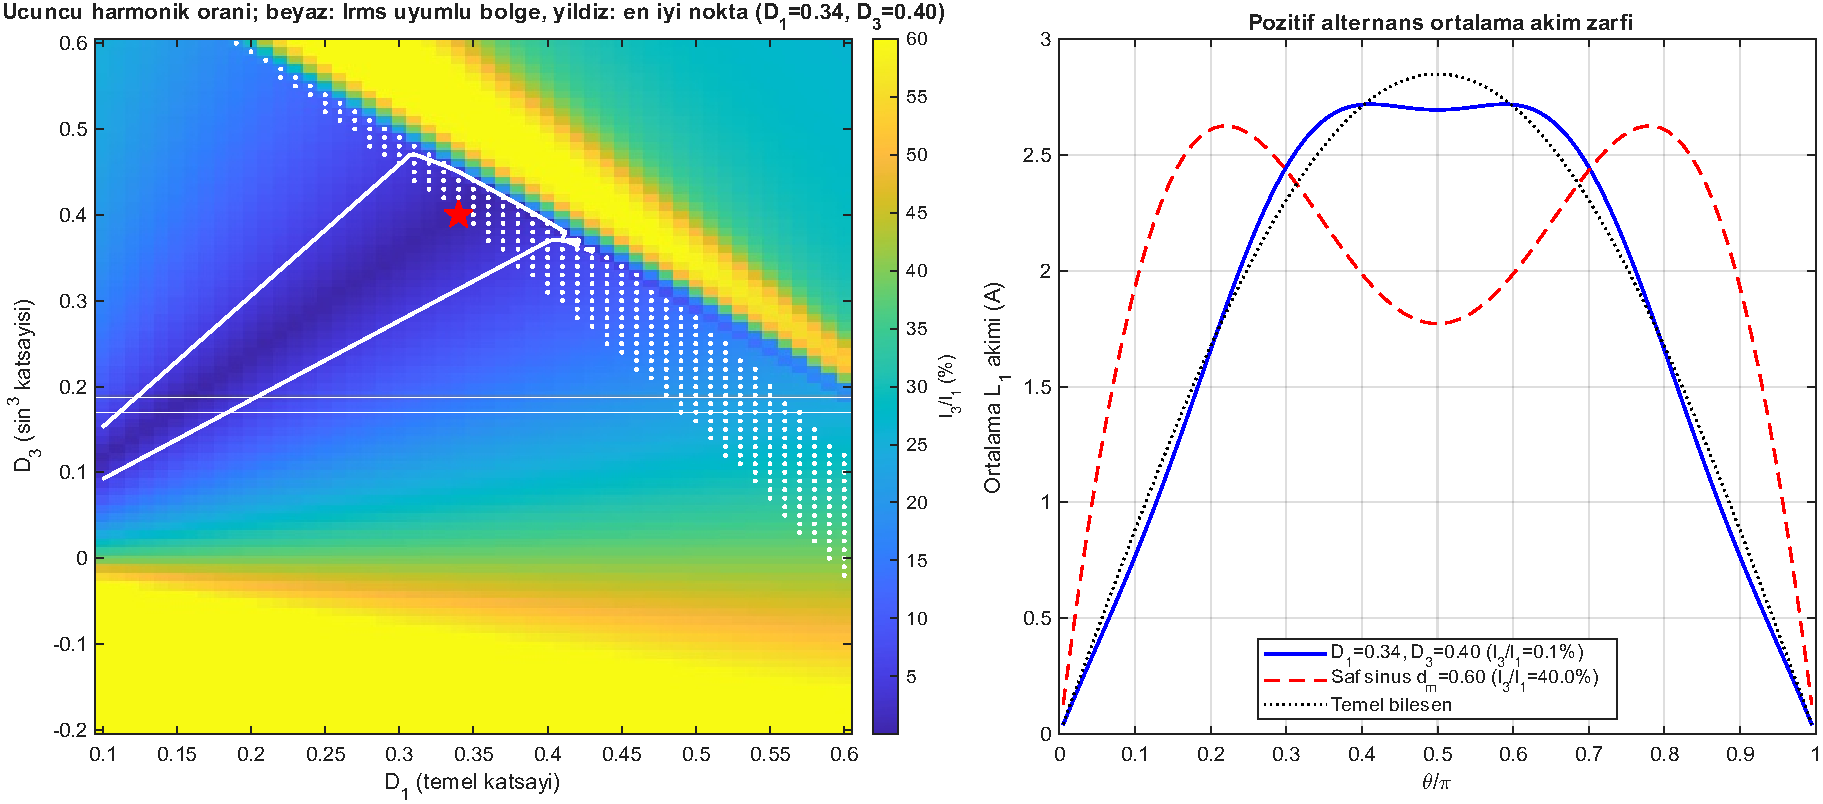
\includegraphics[width=\textwidth]{../tez-matlab-simulink/results/sin3_rescan_20260901/sin3_katsayi_taramasi_20260901.pdf}
  \caption{$(D_1,D_3)$ katsayı düzleminde üçüncü harmonik oranı (sol; beyaz noktalar \SI{2.0}{}--\SI{2.6}{\ampere} RMS bölgesini, yıldız en iyi noktayı gösterir) ve en iyi nokta ile saf sinüs görev oranının ortalama akım zarfı karşılaştırması (sağ). Parçalı DCM/CCM analitik modeli, 01.09.2026 hesabı.}
  \label{fig:sin3-yeniden-tarama}
\end{figure}

Eşitlik~\eqref{eq:sin3-duzeltilmis-optimum} ile verilen çift, uygulanan kazanç değil, tek endüktanslı analitik katmanın adayıdır. Anahtarlamalı benzetimde kullanılan S3 katsayıları ($K_{13}$, $K_{33}$) Alt Bölüm~\ref{sec:kalibrasyon} içinde deney özetinin aktif ve reaktif gücüne kalibre edilmiştir ve harmonik eşdeğerleri $(K_{13}+3K_{33}/4,\ -K_{33}/4)=(0{,}7317,\ -0{,}0961)$'dir. Üçüncü harmonik katsayıları iki katmanda birbirine yakındır ($-0{,}10$ ile $-0{,}096$); temel katsayıdaki fark ($0{,}64$ ile $0{,}73$), analitik modelin içermediği $C_f$--$L_2$ ağı, ölü zaman, kayıplar ve köprünün süreksiz iletimdeki yumuşak gerilim kaynağı davranışından (Alt Bölüm~\ref{sec:kalibrasyon}) kaynaklanır ve analitik adayın \SI{2.02}{\ampere}, kalibre noktanın \SI{2.28}{\ampere} RMS akımda tanımlı olduğu da göz önünde tutulmalıdır. İki katsayı takımının karşılaştırması bir doğrulama değil, analitik katmanın üçüncü harmonik ihtiyacını doğru büyüklükte öngördüğüne ilişkin bir tutarlılık gözlemidir.

\section{Önerilen Yapı ve İleri Besleme Mekanizması}

İleri besleme yolunun fiziksel işlevi, evirici tarafındaki eşdeğer kaynak gerilimini şebeke gerilimine yaklaştırmaktır. PLL şebekeye kilitlendikten sonra, akım komutu uygulanmadan önce, evirici çıkışı ile şebeke eşpotansiyel ise seri $Z_1+Z_2$ filtre ve şebeke empedansından akan akım sıfıra yaklaşır. Şekil~\ref{fig:espotansiyel}, eşpotansiyel durumu eşdeğer kaynaklar ve iki kaynağın eşit gerilim dalga biçimleri üzerinde göstermektedir. Akım referansı uygulandığında denetleyicinin üretmesi gereken ek gerilim yalnız empedans düşümünü karşılayan küçük bir bileşendir; akım küçüldükçe ek bileşen mutlak olarak küçülür ve modeldeki küçük gerilim hataları göreli olarak daha görünür hâle gelir. İleri besleme teriminin düşük akımdaki göreli önemi aynı mekanizmadan kaynaklanır.

\begin{figure}[H]
  \centering
  \resizebox{\textwidth}{!}{%
  \begin{tikzpicture}[font=\small, x=1mm, y=1mm,
    tel/.style={thick},
    emp/.style={draw, thick, fill=white, minimum width=12mm, minimum height=5mm, inner sep=1pt}]
    % eşdeğer devre
    \draw[tel] (0,0) -- (0,30) -- (60,30) -- (60,0) -- cycle;
    \node[emp] at (20,30) {$Z_1$};
    \node[emp] at (42,30) {$Z_2$};
    \draw[thick, fill=white] (0,15) circle (5); \draw (-2.5,15) sin (-1.25,16.5) cos (0,15) sin (1.25,13.5) cos (2.5,15);
    \draw[thick, fill=white] (60,15) circle (5); \draw (57.5,15) sin (58.75,16.5) cos (60,15) sin (61.25,13.5) cos (62.5,15);
    \node[left] at (-6,15) {$v_{\mathrm{inv}}$};
    \node[right] at (66,15) {$v_g$};
    \draw[-{Latex[length=2mm]}, thick, red!70!black] (28,34) -- node[above]{$i=(v_{\mathrm{inv}}-v_g)/(Z_1+Z_2)=0$} (36,34);
    \node[align=center, font=\footnotesize] at (30,-6) {evirici eşdeğer kaynağı \hspace{14mm} şebeke};
    % dalga biçimleri
    \begin{scope}[xshift=82mm, yshift=18mm]
      \draw[-{Latex[length=1.5mm]}] (0,0) -- (52,0) node[right]{$t$};
      \draw[-{Latex[length=1.5mm]}] (0,-13) -- (0,14) node[above]{$v$};
      \draw[very thick, blue!70!black] plot[domain=0:50, samples=80] (\x, {11*sin(9*\x)});
      \draw[thick, dashed, orange!90!black] plot[domain=0:50, samples=80] (\x, {11*sin(9*\x)});
      \node[font=\footnotesize, align=left, anchor=west] at (2,-17) {\textcolor{blue!70!black}{---} $v_{\mathrm{inv}}$ \quad \textcolor{orange!90!black}{-\,-} $v_g$};
    \end{scope}
    \begin{scope}[xshift=82mm, yshift=-12mm]
      \draw[-{Latex[length=1.5mm]}] (0,0) -- (52,0) node[right]{$t$};
      \draw[-{Latex[length=1.5mm]}] (0,-5) -- (0,6) node[above]{$i$};
      \draw[very thick, red!70!black] (0,0) -- (50,0);
      \node[font=\footnotesize, anchor=west] at (2,3) {$i=0$};
    \end{scope}
  \end{tikzpicture}%
  }
  \caption[Eşpotansiyel evirici ve şebeke kaynakları]{İleri beslemenin eşpotansiyel durumu: evirici eşdeğer kaynağı ile şebeke kaynağı aynı genlik ve fazda olduğunda seri $Z_1$ (filtre) ve $Z_2$ (şebeke) empedanslarından akım akmaz. Şekil, akım komutu öncesindeki başlangıç durumunun ideal çözümüdür; kapalı çevrim izleme başarımını göstermez.}
  \label{fig:espotansiyel}
\end{figure}

Denetleyicinin devre dışı bırakılıp yalnız ileri besleme katsayısının değiştirildiği benzetim koşulu, yöntemin açık çevrim mekanizmasını ayırmak için yararlıdır; ancak kapalı çevrim başarımı ya da kararlılık kanıtı değildir. Şebeke gerilimi ileri beslemesi ideal durumda evirici ile şebeke gerilimini yaklaştırarak düşük akımdaki göreli gerilim hatasını azaltabilir; LCL filtre, ortak bağlantı noktası ölçümü ve sayısal gecikme eklendiğinde aynı yol sanal empedans ve aktif sönümleme etkisi de oluşturabilir \citep{Lu2016}. İleri besleme yolunun etkisi yalnız gerilim düşümü hesabıyla sınırlandırılmamıştır. Sin\textsuperscript{3} yolunun modülasyon toplamındaki konumu Şekil~\ref{fig:denetim-modulasyon-blok} üzerinde verilmiştir.

\section{Senaryo~3 Benzetim Kayıtları}
\label{sec:sin3-senaryo3-kayitlari}

Şekil~\ref{fig:s3-kalibre-l1}, kalibre S3 modelinde $L_1$ akımını ve şebeke akımını gösterir. Sin\textsuperscript{3} terimi, S2'de alternans ortasında çöken şebeke akımı zarfını sinüse yaklaştırır; $L_1$ akımı susturmalı çalışmanın süreksiz iletim yapısını korur, ters akım aralığı yoktur ve pozitif yarım periyodun \%27,6'sında akım sıfırdadır. Kompanzasyon süreksiz iletimi ortadan kaldırmaz; darbe genişliklerini, süreksiz iletimin ürettiği üçüncü harmoniği karşılayacak biçimde değiştirir.

\begin{figure}[H]
  \centering
  \includegraphics[width=0.96\textwidth]{model_dogrulama/s3_kalibre_l1.pdf}
  \caption[Kalibre benzetimde S3 $L_1$ akımı]{Kalibre benzetimde S3 (susturma + Sin\textsuperscript{3}): (a) son tam şebeke periyodunda $i_{L1}$, şebeke akımı $i_g$ ve karşılaştırma için S2 şebeke akımı; (b) pozitif yarım periyottan \SI{400}{\micro\second} kesitte $i_{L1}$.}
  \label{fig:s3-kalibre-l1}
\end{figure}

Kalibre S3 modeli deneydeki \%14 akım THD'sini \%14,8 ile yeniden üretmektedir (Alt Bölüm~\ref{sec:kalibrasyon}). Deneyde susturma THD'yi \%15'ten \%47'ye çıkarmış, Sin\textsuperscript{3} terimi \%14'e indirmiştir; S3, klasik anahtarlamanın harmonik düzeyine dönerken verimi klasik anahtarlamadan 2,0 puan yüksek tutmaktadır. Sonuç, Sin\textsuperscript{3} yolunun üçüncü harmonik cezasını önemli ölçüde azalttığını destekler. S1, S2 ve S3 deneylerinin DA bara gerilimleri (\SI{431.5}{}, \SI{395.0}{} ve \SI{427.5}{\volt}) ve şebeke gerilimleri (\SI{119.8}{}, \SI{121.0}{} ve \SI{124.3}{\volt}) birbirinden farklıdır (Tablo~\ref{tab:sistem-parametreleri}, Tablo~\ref{tab:deney-kosullari}). Her benzetim kendi deneyinin DA bara ve şebeke gerilimiyle yapılmıştır; deney ile benzetim aynı koşuldadır, ancak üç yöntem birbirinden farklı gerilimlerde çalıştığı için yöntemler arası karşılaştırma tek değişkenli değildir.

\section{Senaryo~4: Akım Geri Beslemeli Kapalı Çevrim}
\label{sec:s4-kapali-cevrim}

Senaryo~1--3 açık çevrim modülasyonla, deney donanımının yaklaşık \SI{2.3}{\ampere} faz akımında çalışmaktadır. Nötr susturma ve Sin\textsuperscript{3} ileri beslemesinin anma akımına taşınıp taşınamayacağı ve akım denetimiyle birlikte nasıl davrandığı Senaryo~4 (S4) ile incelenmiştir. S4, S3 modeline $L_1$ akımı geri beslemesi eklenerek kurulmuştur; güç katı ve ölçüm blokları S3 ile aynıdır (Şekil~\ref{fig:s3-simulink-modeli}), fark anahtarlama girişindedir (Şekil~\ref{fig:s4-anahtarlama-girisi}). Model çiziminde geri besleme oransal kazançla gösterilmiştir; tezdeki S4 benzetimlerinde denetleyici S3 tabanına betikle eklenmiş ve oransal denetleyiciye ek olarak PI ve PIR seçenekleriyle kurulmuştur (Alt Bölüm~\ref{sec:model-dogrulama-duzeltme}).

\begin{figure}[H]
  \centering
  \includegraphics[width=0.82\textwidth]{umit_2026-11-09/s4_anahtarlama_girisi.pdf}
  \caption[S4 modelinin anahtarlama girişi]{S4 modelinin anahtarlama girişi: Sin\textsuperscript{3} ileri beslemesi ($K_{14}$, $K_{34}$), $L_1$ akımı geri beslemeli oransal denetleyici ($K_p$), doyum ve kapı mantığı alt sistemi (\textsc{anahtarlama}). Güç katı ve ölçüm blokları Şekil~\ref{fig:s3-simulink-modeli} ile aynıdır.}
  \label{fig:s4-anahtarlama-girisi}
\end{figure} S4 için donanım deneyi yoktur; Alt Bölüm~\ref{sec:s4-kapali-cevrim} içindeki bütün sayılar benzetim sonucudur ve kalibre S3 modelinin kapalı çevrimle anma akımına taşınmasını gösterir.

\subsection{Model ve denetleyici yapısı}

S4 modülasyon komutu, ileri besleme ve geri besleme terimlerinin doyumlu toplamıdır:
\begin{equation}
  \begin{gathered}
    u=\operatorname{sat}_{\pm1}\!\left(u_{\mathrm{ff}}+u_{\mathrm{fb}}\right),\qquad
    u_{\mathrm{ff}}=K_{14}\sin(\theta+\varphi_4)+K_{34}\sin^3(\theta+\varphi_4),\\
    u_{\mathrm{fb}}=C(s)\left[i_{\mathrm{ref}}-H_m(s)\,i_{L1}\right],\qquad
    i_{\mathrm{ref}}=\sqrt2\,I_{\mathrm{ref}}\sin\theta .
  \end{gathered}
  \label{eq:s4-denetim-yapisi}
\end{equation}
Eşitlik~\eqref{eq:s4-denetim-yapisi} içinde $\theta$ şebekeye kilitli açı (ideal PLL), $H_m(s)$ tek kutuplu ölçüm süzgeci ve $C(s)$ akım denetleyicisidir. İleri besleme kazançları $K_{14}$, $K_{34}$ ve faz $\varphi_4$, kalibre S3 değerleridir (Tablo~\ref{tab:sistem-parametreleri}). Üç denetleyici aynı alt sistemde kazanç seçimiyle gerçeklenmiştir:
\begin{equation}
  C_{\mathrm{P}}(s)=K_p,\qquad
  C_{\mathrm{PI}}(s)=K_p+\frac{K_i}{s},\qquad
  C_{\mathrm{PIR}}(s)=C_{\mathrm{PI}}(s)+\frac{2K_r\omega_b s}{s^2+2\omega_b s+\omega_0^2}.
  \label{eq:s4-denetleyiciler}
\end{equation}
Oransal kazanç parametre dosyasındaki değerdir. PI sıfırı \SI{60}{\hertz}'e, yani birinci kazanç geçiş frekansının (yaklaşık \SI{586}{\hertz}, Tablo~\ref{tab:kararlilik-marjlar}) yaklaşık onda birine yerleştirilmiştir; \SI{60}{\hertz} değerinin şebeke frekansıyla ilgisi yoktur. Sıfırın geçiş frekansının onda birinde olması, integral teriminin geçişte getirdiği faz kaybını $\arctan(60/586)\simeq6^{\circ}$ ile sınırlar; P ve PI çevrimlerinin birinci geçişteki faz marjı farkı $5{,}9^{\circ}$'dir. PI denetleyicinin doyum önlemesi geri hesaplama yöntemiyle kurulmuştur. Kazançların tamamı Tablo~\ref{tab:sistem-parametreleri} içindeki S4 akım denetimi grubundadır. Denetim, modelde analog eşdeğeri olarak gerçeklenmiştir: denetleyici \SI{1}{\micro\second} adımla çalışır ve hesaplama gecikmesi yoktur. Analog eşdeğerin seçilme gerekçesi, PWM periyodu başında örnekleyip bir periyot gecikmeyle uygulayan sayısal gerçeklemenin LCL rezonansında kararsız olmasıdır; gerekçe Alt Bölüm~\ref{sec:kararlilik-bode} içinde sayısal olarak verilmektedir. $L_1$ doyumu modellenmemiştir.

\textbf{DA bara önkoşulu.} Faz başına modelde faz akımının tamamı bara kapasitörlerinden geçtiği için orta nokta salınımı akımla büyür (Alt Bölüm~\ref{sec:model-dogrulama-duzeltme}). Faz başına modelin bara kapasitörleri (2$\times$\SI{470}{\micro\farad}) üç fazlı deney donanımının toplam bara kapasitansından bir faza düşen paydır; üç fazlı donanımda toplam kapasitans faz payının üç katıdır. Faz payı kapasitansla modeldeki salınım \SI{2.3}{\ampere}'de yaklaşık \SI{11}{\volt} ($V_{\mathrm{dc}}/2$'nin \%5'i), \SI{25}{\ampere}'de ise yaklaşık \SI{120}{\volt} (\%56) olmaktadır. Faz payı kapasitansla yapılan PI benzetiminde evirici darbe yüksekliği pozitif alternans boyunca yaklaşık \SI{270}{\volt}'tan \SI{100}{\volt}'a inmiş, modülasyon zamanın \%20,6'sında doyuma girmiş ve kararlı durum oluşmamıştır: temel akım genlik hatası $-$\%31,9, THD \%57,4'tür. Orta nokta salınımı faz başına modelde \SI{25}{\ampere}'de büyüdüğü için S4 anma akımı benzetimlerinde bara kapasitansı 2$\times$\SI{5.6}{\milli\farad} değerine büyütülmüş ve salınım yaklaşık \SI{10}{\volt}'a (\%4,7) inmiştir (Tablo~\ref{tab:sistem-parametreleri}). Aynı PI denetleyicide genlik hatası $-$\%2,1'e, THD \%9,2'ye iner ve doyum ortadan kalkar. Anma akımında kapalı çevrim çalışmanın önkoşulu, DA bara orta noktasının tutulabilmesidir; büyütülmüş kapasitans değeri donanımda doğrulanmamıştır.

\subsection{Düşük, orta ve anma akımı taraması}

Tablo~\ref{tab:s4-tarama}, büyütülmüş DA bara ve kalibre ileri beslemeyle yapılan kesin taramayı vermektedir. Kararlı durum büyüklükleri son tam şebeke periyodundan alınmıştır; P ve PI benzetimleri \SI{0.06}{\second}, PIR benzetimleri rezonans teriminin dar bandı nedeniyle \SI{0.2}{\second} sürmüştür. Oturma ölçütü olarak son iki periyodun aktif güç farkı kullanılmış, tablodaki bütün benzetimlerde fark \%0,12'nin altında kalmıştır. Verim sütunu modelin DA ve AA güç ölçüm bloklarından alınmıştır. S4, $L_1$ çekirdek kaybı için S1--S3'ten farklı bir paralel direnç kullandığından (Tablo~\ref{tab:sistem-parametreleri}) S4 verimi yalnız S4 içinde karşılaştırılır; yaklaşık \SI{280}{\watt} çıkışta S4 verimi \%96,2, kalibre S3 verimi \%94,25'tir ve aradaki farkın yaklaşık \SI{7.2}{\watt}'lık kayıp karşılığı yalnız çekirdek kaybı parametresinden gelir.

\begin{table}[H]
  \centering
  \caption{S4 kapalı çevrim benzetimi: düşük, orta ve anma akımında akım izleme, harmonik, verim ve doyum (büyütülmüş DA bara, kalibre ileri besleme). PIR benzetimleri \SI{0.2}{\second}, diğerleri \SI{0.06}{\second}.}
  \label{tab:s4-tarama}
  \footnotesize
  \setlength{\tabcolsep}{2.6pt}
  \begin{tabular}{@{}l c c r r r r r c c@{}}
    \toprule
    Den., $I_{\mathrm{ref}}$ & $I_{L1,1}$ (A) & Genlik h. & Faz h. & THD$_I$ & $I_3/I_1$ & $P_{\mathrm{ac}}$ (W) & $\eta$ & Doyum & $|u|_{\max}$ \\
    \midrule
    P, \SI{2.3}{\ampere}   & 2,336 & $+$\%1,6  & $+1{,}0^{\circ}$ & \%7,0  & \%6,5  & 280,7 & \%96,24 & \%0 & 0,86 \\
    PI, \SI{2.3}{\ampere}  & 2,327 & $+$\%1,2  & $+1{,}4^{\circ}$ & \%7,2  & \%6,6  & 279,5 & \%96,20 & \%0 & 0,86 \\
    \midrule
    P, \SI{10}{\ampere}    & 7,677 & $-$\%23,2 & $-1{,}1^{\circ}$ & \%22,6 & \%20,9 & 922,5 & \%97,44 & \%0 & 0,87 \\
    PI, \SI{10}{\ampere}   & 8,918 & $-$\%10,8 & $-6{,}3^{\circ}$ & \%20,8 & \%18,7 & 1065  & \%97,31 & \%0 & 0,88 \\
    PIR, \SI{10}{\ampere}  & 9,777 & $-$\%2,2  & $+0{,}4^{\circ}$ & \%19,6 & \%18,7 & 1175  & \%97,28 & \%0 & 0,87 \\
    \midrule
    P, \SI{25}{\ampere}    & 22,15 & $-$\%11,4 & $-2{,}6^{\circ}$ & \%9,8  & \%9,6  & 2662  & \%96,69 & \%0 & 0,90 \\
    PI, \SI{25}{\ampere}   & 24,47 & $-$\%2,1  & $-4{,}0^{\circ}$ & \%9,2  & \%8,7  & 2938  & \%96,45 & \%0 & 0,90 \\
    PIR, \SI{25}{\ampere}  & 24,75 & $-$\%1,0  & $+0{,}2^{\circ}$ & \%8,5  & \%8,1  & 2978  & \%96,03 & \%0 & 0,93 \\
    \bottomrule
  \end{tabular}
\end{table}

\umitnot{İstenen THD sınırına ulaşıldı mı?}{Tezde şebeke standardıyla sayısal karşılaştırma yoktur; aşağıdaki hesap bilgi içindir. IEEE~1547 ve IEC~61727, toplam harmonik bozulmayı anma akımına göre (TDD) \%5, tek mertebeli 3--9. harmoniklerin her birini \%4 ile sınırlar. Anma akımı \SI{25}{\ampere} alınmıştır.
\begin{itemize}\setlength{\itemsep}{1pt}
  \item \textbf{\SI{2.3}{\ampere} (deney noktası): sınır içinde.} Harmonik akım anma akımının küçük bir kesridir. TDD: S1 yaklaşık \%1,3 (deneyin \%15'iyle; kalibre modelin \%39,5'iyle yaklaşık \%3,4), S2 yaklaşık \%4,0 (kalibre model \%4,8, sınıra yakın), S3 yaklaşık \%1,3. THD kendi temel bileşenine göre okunursa hiçbir senaryo \%5'e inmez; en iyisi S3, \%14.
  \item \textbf{\SI{10}{\ampere}: sınır dışı.} THD yaklaşık \%20, TDD yaklaşık \%7--8. Nedeni nötr susturmanın orta akımda çevrimin büyük kısmında süreksiz iletim yaratmasıdır.
  \item \textbf{\SI{25}{\ampere} (anma): sınır dışı.} THD PI ile \%9,2, PIR ile \%8,5; üçüncü harmonik \%8,7 ile tekil \%4 sınırını da aşar. Sin\textsuperscript{3} kazancı \SI{2.3}{\ampere}'e kalibre edildiğinden anma akımında üçüncü harmoniği artırır; terim kapatıldığında THD \%5,6'ya iner, yine sınırın biraz üstündedir.
  \item \textbf{Tezdeki yeri.} Orta akımda süreksiz iletim ve anma akımında ileri besleme genliği Bölüm~\ref{chap:sonuc} sınırlılıklarında (madde 5 ve 6) yazılıdır. Anma akımında sınırın altına inmek için akıma göre ayarlanan Sin\textsuperscript{3} genliği ya da susturmadan tamamlayıcı anahtarlamaya geçiş gerekir; ikisi de gelecek çalışma olarak önerilmiştir.
\end{itemize}}

Anma akımında PI ve PIR denetleyicileri referansı doyumsuz izlemektedir. PIR, \SI{50}{\hertz} rezonans terimiyle temel bileşen hatasını $-$\%1,0 ve $+0{,}2^{\circ}$'ye indirir; THD \%8,5, temel bileşen güç faktörü ($\cos\varphi_1$) 0,997'dir. Oransal denetleyici aynı noktada $-$\%11,4 genlik hatası bırakır; \SI{50}{\hertz}'teki sonlu çevrim kazancı kalıcı hatayı sıfırlamaz. Şekil~\ref{fig:s4-akim-izleme-25a}, \SI{25}{\ampere} noktasında üç denetleyicinin son iki şebeke periyodundaki $L_1$ akımını, referansı, çıkış akımını ve C noktası gerilimini birlikte göstermektedir; gerilim sağ eksende, şebeke nötrüne göre çizilmiştir. Şekil~\ref{fig:s4-tarama-ozet} ise verim, THD ve genlik hatasının akıma göre değişimini özetlemektedir.

\begin{figure}[H]
  \centering
  \includegraphics[width=\textwidth,height=0.62\textheight,keepaspectratio]{s4/s4_akim_izleme_25A_KC.pdf}
  \caption{S4 benzetiminde \SI{25}{\ampere} anma akımında P (üst), PI (orta) ve PIR (alt) denetleyicileriyle $L_1$ akımı (anlık ve anahtarlama periyodu ortalaması), akım referansı, çıkış akımı (sol eksen) ve şebeke nötrüne göre C noktası gerilimi $v_{ac}$ (sağ eksen, eksen sıfırları hizalı); son iki şebeke periyodu. Üç denetleyicide de $v_{ac}$'nin periyot ortalaması \SI{0.03}{\volt} altındadır.}
  \label{fig:s4-akim-izleme-25a}
\end{figure}

\begin{figure}[H]
  \centering
  \includegraphics[width=\textwidth]{s4/s4_tarama_ozet_KC.pdf}
  \caption{S4 benzetiminde verim, akım THD'si ($h\leq50$) ve temel bileşen genlik hatasının akım referansına göre değişimi; P, PI ve PIR denetleyicileri.}
  \label{fig:s4-tarama-ozet}
\end{figure}

\textbf{Orta akımda süreksiz iletim.} İzleme hatası akımla monoton değişmemektedir: \SI{10}{\ampere} noktası \SI{25}{\ampere} noktasından kötüdür. $L_1$ akım dalgalanması yaklaşık \SI{9}{\ampere} tepeden tepeye olduğundan anlık akımın mutlak değeri yaklaşık \SI{4.5}{\ampere}'in altına indiği her bölgede nötr susturmalı köprü süreksiz iletime girer ve senkron olmayan buck gibi davranır (Alt Bölüm~\ref{sec:dusuk-akim-modelleme}). \SI{25}{\ampere}'de süreksiz bölge yalnız sıfır geçişleri çevresindedir; \SI{10}{\ampere}'de ise çevrimin büyük kısmını kaplar. \SI{10}{\ampere}'de üçüncü harmonik baskındır ($I_3/I_1$ \%19--21). Kalibre Sin\textsuperscript{3} terimi \SI{2.3}{\ampere} noktasındaki bozulmaya göre ayarlandığından, süreksiz iletim bölgesi akımla değiştiğinde aynı terim \SI{10}{\ampere} noktasına uymamaktadır. PI'nin integral terimi genlik hatasını $-$\%23'ten $-$\%11'e indirir; PIR temel bileşeni $-$\%2,2 ve $+0{,}4^{\circ}$ ile kapatır, ancak THD \%19,6'da kalır, çünkü rezonans terimi yalnız \SI{50}{\hertz}'te etkilidir ve üçüncü harmonik bozulması süreksiz iletimden gelmektedir. Kararlılık analizi (Alt Bölüm~\ref{sec:kararlilik-bode}), \SI{10}{\ampere}'deki genlik hatasının bir kararlılık sorunu değil, köprünün etkin kazancındaki düşüşten doğan bir izleme sorunu olduğunu göstermektedir. Nötr susturma bir düşük güç yöntemidir: orta ve anma akımında tamamlayıcı anahtarlamaya dönüş ya da akım düzeyine göre ayarlanan ileri besleme gerekir. Kip geçişi tezin kapsamı dışındadır ve Bölüm~\ref{chap:sonuc} içinde öneri olarak yer almaktadır.

\subsection{Basamak yanıtı}

PI denetleyiciyle akım referansı $t=\SI{55}{\milli\second}$ anında \SI{10}{\ampere}'den \SI{25}{\ampere}'e basamak olarak değiştirilmiştir. Tablo~\ref{tab:s4-basamak} sonuçları vermektedir. Aşım, $L_1$ akım zarfının basamak sonrasındaki en büyük tepesinin son kararlı zarfa oranı olarak tanımlanmıştır. Kararlı durumda bile $L_1$ akımının tepesi, Sin\textsuperscript{3} kaynaklı üçüncü harmonik nedeniyle referans tepesinden \%7,3 yüksektir; aşım referans tepesine göre tanımlansaydı kararlı durumdaki dalga biçimi aşım gibi sayılırdı. Basamak sonrası kararlı değer, doğrudan \SI{25}{\ampere}'de başlatılan PI benzetimiyle aynıdır (\SI{24.48}{\ampere} ve \SI{24.47}{\ampere}); çözüm başlangıç koşulundan bağımsızdır. Basamak süresince geçici bileşenin sönümü Şekil~\ref{fig:s4-basamak} üzerinde, $K_{34}$ açık ve kapalı karşılaştırması ise Alt Bölüm~\ref{sec:kararlilik-bode} içinde verilmektedir.

\begin{table}[H]
  \centering
  \caption{S4 benzetiminde PI denetleyiciyle \SI{10}{\ampere}$\rightarrow$\SI{25}{\ampere} referans basamağı.}
  \label{tab:s4-basamak}
  \small
  \begin{tabularx}{0.9\textwidth}{@{}X r@{}}
    \toprule
    Büyüklük & Değer \\
    \midrule
    Basamak öncesi $I_{L1,1}$ (referans \SI{10}{\ampere}) & \SI{8.91}{\ampere} \\
    Basamak sonrası $I_{L1,1}$ (referans \SI{25}{\ampere}) & \SI{24.48}{\ampere} ($-$\%2,1) \\
    Aşım (son kararlı zarfa göre) & \%0,2 \\
    $L_1$ akım tepesinin referans tepesine oranı (kararlı durum, üçüncü harmonik dahil) & \%7,3 üstünde \\
    Yerleşme süresi (hata bandı) & \SI{0.44}{\milli\second} \\
    Geçişte doyum & zamanın \%0,8'i; $|u|_{\max}=1{,}49$ \\
    Basamak sonrası THD$_I$ & \%9,1 \\
    \bottomrule
  \end{tabularx}
\end{table}

\begin{figure}[H]
  \centering
  \includegraphics[width=\textwidth,height=0.5\textheight,keepaspectratio]{s4/s4_basamak_PI_10_25A_KC.pdf}
  \caption{S4 benzetiminde PI denetleyiciyle \SI{10}{\ampere}$\rightarrow$\SI{25}{\ampere} akım referansı basamağı: $L_1$ akımı, anahtarlama periyodu ortalaması ve modülasyon komutu.}
  \label{fig:s4-basamak}
\end{figure}

\section{Kararlılık ve Bode Analizi}
\label{sec:kararlilik-bode}

Sin\textsuperscript{3} yönteminin kapalı çevrim kararlılığı üç katmanda incelenmiştir. Birinci katman, Sin\textsuperscript{3} teriminin karakteristik denklemde yer almadığını analitik olarak gösterir. İkinci katman, S4 akım çevriminin açık çevrim kazancı $L$, duyarlılık fonksiyonu $S$ ve tamamlayıcı duyarlılık fonksiyonu $T$ için Bode eğrilerini, kazanç ve faz marjlarını ve kapalı çevrim kutuplarını $K_{34}$ açık ve kapalı hesaplar. Üçüncü katman, anahtarlamalı S4 modelinde küçük işaret enjeksiyonuyla ölçülen çevrim kazancını ve basamak yanıtını ortalama modelle karşılaştırır. Bütün sonuçlar benzetim modelinin kendi içindeki kararlılık kanıtıdır; S4 için donanım deneyi yoktur.

\subsection{Analitik katman: Sin\texorpdfstring{\textsuperscript{3}}{3} terimi çevrimin dışındadır}

Denetlenen sistem $G(s)=i_{L1}/v_{\mathrm{inv}}$, evirici kutup geriliminden $L_1$ akımına ortalama aktarım fonksiyonudur ve güç ağı anahtarlamalı modeldeki sırayla kurulmuştur: $L_1$ ve çekirdek kaybı direnci, $C_f$, EMC süzgecinin diferansiyel kip endüktansları ve X kapasitörü, $L_2$ ve şebeke (Tablo~\ref{tab:sistem-parametreleri}). Antirezonans (anti-resonance), LCL filtrede evirici geriliminden evirici tarafı ($L_1$) akımına giden yolun kazancının çöktüğü frekanstır; $C_f$ ile $L_2$'nin paralel rezonansına karşılık gelir ve yaklaşık $f_{\mathrm{antirez}}\simeq1/(2\pi\sqrt{L_2C_f})$ ile verilir. Ortalama modeldeki denetlenen sistemin rezonansı \SI{2815}{\hertz} ($\zeta=0{,}0041$), antirezonansı \SI{1720}{\hertz}'tir; antirezonans, $C_f$'ye EMC süzgecinin X kapasitörü eklendiği için yaklaşık ifadenin verdiği \SI{1.78}{\kilo\hertz}'in biraz altındadır. Normalize modülasyon komutunu kutup gerilimine dönüştüren PWM kazancı $K_{\mathrm{pwm}}=V_{\mathrm{dc}}/2$, toplam gecikme $T_d$ ve şebeke geriliminden akıma aktarım $G_g(s)$ ile gösterilsin. Açık çevrim (çevrim) kazancı $L$, çevrim bir noktadan açıldığında işaretin çevrimi bir kez dolaşırken uğradığı toplam kazançtır. Duyarlılık fonksiyonu $S=1/(1+L)$, bozucuların ve izleme hatasının çevrimce ne ölçüde bastırıldığını; tamamlayıcı duyarlılık fonksiyonu $T=L/(1+L)$ ise referansın çıkışa ne ölçüde aktarıldığını gösterir. $|S|\ll1$ olan frekanslarda bozucu bastırılır, $|T|\simeq1$ olan frekanslarda referans izlenir. Doyum dışında Eşitlik~\eqref{eq:s4-denetim-yapisi} çevrimi
\begin{equation}
  L(s)=C(s)\,K_{\mathrm{pwm}}\,e^{-sT_d}\,G(s)\,H_m(s)
  \label{eq:sin3-acik-cevrim}
\end{equation}
açık çevrim kazancını tanımlar. Duyarlılık ve tamamlayıcı duyarlılık fonksiyonları
\begin{equation}
  S(s)=\frac{1}{1+L(s)},
  \qquad
  T(s)=\frac{L(s)}{1+L(s)}
  \label{eq:sin3-duyarlilik}
\end{equation}
biçimindedir. Kapalı çevrimde $L_1$ akımı
\begin{equation}
  i_{L1}=\frac{K_{\mathrm{pwm}}e^{-sT_d}G(s)\left[u_{\mathrm{ff}}+C(s)\,i_{\mathrm{ref}}\right]+G_g(s)\,v_g}{1+L(s)}
  \label{eq:sin3-kapali-cevrim-girisleri}
\end{equation}
olarak yazılır. $\theta$ yalnız zamana bağlıdır ve şebekeye kilitlidir; $\sin^3\theta$ işaretinin hiçbir girişi çevrimdeki bir büyüklükten gelmez. Eşitlik~\eqref{eq:sin3-kapali-cevrim-girisleri} içinde $u_{\mathrm{ff}}$ yalnız payda, dış bir giriş olarak yer alır; karakteristik denklem $1+L(s)=0$, $K_{34}$'ü içermez. Kapalı çevrim kutupları, kazanç ve faz marjları $K_{34}$'ten bağımsızdır; $K_{34}$ yalnız dış girişin genliğini değiştirir. Doyum sınırı bütün kararlı durum pencerelerinde aşılmamıştır ($|u|_{\max}\leq0{,}93$, Tablo~\ref{tab:s4-tarama}); doyumsuz çalışmada doğrusal ayrım çalışma noktalarında geçerlidir.

Sin\textsuperscript{3} teriminin akıma etkisi $S(j\omega)K_{\mathrm{pwm}}G(j\omega)$ ile belirlenir. Eşitlik~\eqref{eq:sin3-esdeger-katsayilar} ile kalibre ileri besleme $0{,}7317\sin(\theta+\varphi_4)-0{,}0961\sin(3\theta+3\varphi_4)$ biçimindedir. PI denetleyicide $|S(j2\pi\cdot\SI{150}{\hertz})|=0{,}234$ ($-12{,}6$~dB) olduğundan, üçüncü harmonik modülasyonun çevrimsiz durumda üreteceği \SI{9.53}{\ampere} RMS \SI{150}{\hertz} akımı çevrim \SI{2.23}{\ampere} RMS'ye indirir; P ve PIR için oran 0,231 ve 0,214'tür. Temel bileşende Sin\textsuperscript{3}'ün payı ($3K_{34}/4$), ortalama modelde PI ile $L_1$ temel akımını \SI{22.71}{\ampere}'den \SI{25.18}{\ampere} RMS'ye taşır. Kapalı çevrimde ileri besleme, denetleyicinin karşılaması gereken temel bileşeni azaltır ve çevrim açısından bilinen bir dış giriştir; çevrimin kendisi, yani $L$, $S$ ve $T$, değişmez.

\subsection{Frekans alanı: marjlar, Bode eğrileri ve kutuplar}

Gerçekleme (A), modeldeki analog eşdeğerdir: sürekli denetleyici, \SI{5}{\kilo\hertz} ölçüm süzgeci ve üst sınır olarak $T_d=\SI{2}{\micro\second}$ toplam gecikme. Aynı yapının \SI{1}{\micro\second} ayrık karşılığı marjları en çok $0{,}02^{\circ}$ ve \SI{0.1}{\decibel} değiştirdiğinden ayrıca tablolanmamıştır. Gerçekleme (B) sayısal bir denetleyiciyi temsil eder: denetim periyodu bir PWM periyodu ($T_s=\SI{100}{\micro\second}$), periyot ortalamalı örnekleme, bir periyotluk hesaplama gecikmesi ve sıfırıncı mertebe tutucu. (B2), aynı yapının periyotta iki güncellemeli ($T_s=\SI{50}{\micro\second}$) biçimidir.

Denetlenen sistemdeki LCL filtre nedeniyle $|L(j\omega)|$ eğrisi 0~dB eksenini üç kez keser: birinci geçişten sonra antirezonansta düşen kazanç, rezonansa doğru yeniden yükselir ve rezonans tepesinden sonra tekrar düşer. Tek bir kesişim frekansıyla verilen marj tanımı eksik kalır. Tezde faz marjı her kazanç geçişi $f_i$ için ayrı hesaplanmıştır: $\mathrm{PM}_i=180^{\circ}-|\angle L(j2\pi f_i)|$; gecikme marjı $\mathrm{DM}_i$, $-1$ noktasına ulaşmak için gereken ek saf gecikmedir. Kazanç marjı, $L$'nin negatif gerçel ekseni kestiği faz geçişinde $\mathrm{GM}=-20\log_{10}|L|$ olarak tanımlanmıştır. LCL rezonansında $L$'nin fazı $0^{\circ}$'dan geçer ve $|L|\simeq\SI{30}{\decibel}$'dir; nokta pozitif gerçel eksendedir ve faz geçişi değildir. Kararlılık hükmü Nyquist ölçütüne dayanır: açık çevrimde kararsız kutup bulunmadığından ($P=0$), $(-\infty,-1)$ ışınının net kesişim sayısı sıfır olmalıdır. Ek olarak kapalı çevrim kutupları doğrudan hesaplanmış ve modül marjı $1/\|S\|_\infty$ verilmiştir. Üç ölçüt her satırda aynı sonucu vermektedir.

\begin{table}[H]
  \centering
  \caption{S4 akım çevriminin marjları (\SI{25}{\ampere}, ortalama model). Nyquist sütunu $(-\infty,-1)$ ışınının net kesişim sayısıdır; 0 kararlı, 1 kararsız. Bütün değerler $K_{34}$ açık ve $K_{34}=0$ için bit düzeyinde aynıdır.}
  \label{tab:kararlilik-marjlar}
  \scriptsize
  \setlength{\tabcolsep}{2.8pt}
  \begin{tabular}{@{}l l c c c r r c c@{}}
    \toprule
    Gerç. & Den. & Kazanç geçişleri (Hz) & $\mathrm{PM}_i$ ($^{\circ}$) & $\mathrm{DM}_{\min}$ (\si{\micro\second}) & Faz geçişi (Hz) & GM (dB) & $\|S\|_\infty$ (dB) & Nyquist \\
    \midrule
    A  & P   & 583 / 2454 / 3386 & 83,6 / 119,4 / 55,2 & 45,3 & 22\,167 & $+$35,3 & 2,28 & 0 \\
    A  & PI  & 586 / 2454 / 3386 & 77,7 / 120,8 / 54,2 & 44,4 & 22\,029 & $+$35,2 & 2,36 & 0 \\
    A  & PIR & 590 / 2454 / 3386 & 73,8 / 121,7 / 53,5 & 43,9 & 21\,937 & $+$35,2 & 2,42 & 0 \\
    \midrule
    B  & P   & 581 / 2474 / 3254 & 48,8 / 90,2 / 142,1 & 101 & 2811 & $-$30,3 & 5,12 & 1 \\
    B  & PI  & 574 / 2479 / 3246 & 43,3 / 88,7 / 142,1 & 99  & 2811 & $-$30,1 & 5,57 & 1 \\
    B  & PIR & 579 / 2479 / 3246 & 39,1 / 88,0 / 142,6 & 99  & 2810 & $-$30,0 & 6,02 & 1 \\
    B2 & PI  & 583 / 2440 / 3444 & 63,7 / 179,4 / 33,3 & 204 & 2863 & $-$20,4 & 4,97 & 1 \\
    \bottomrule
  \end{tabular}
\end{table}

Marj tablosunun satırları iki gerçeklemeyi, analog eşdeğer (A) ile sayısal (B ve B2) gerçeklemeyi, her gerçeklemede de P, PI ve PIR denetleyicilerini karşılaştırır; $K_{34}$ açık ve kapalı değerler bit düzeyinde aynı olduğundan ayrı satır açılmamıştır. Kazanç geçişleri sütunu $|L|=1$ olan frekansları, $\mathrm{PM}_i$ sütunu her geçişteki faz marjını, $\mathrm{DM}_{\min}$ sütunu çevrimin kararlılık sınırına ulaşmadan kaldırabileceği en küçük ek gecikmeyi, faz geçişi ve GM sütunları $\angle L=-180^{\circ}$ noktasındaki kazanç marjını, $\|S\|_\infty$ sütunu ise $L$ eğrisinin $-1$ noktasına en yakın uzaklığının tersini verir. Yaygın tasarım ölçütleri her kazanç geçişinde $\mathrm{PM}_i\gtrsim45^{\circ}$, $\mathrm{GM}\gtrsim\SI{6}{\decibel}$ ve $\|S\|_\infty\lesssim\SI{6}{\decibel}$'dir; $\mathrm{DM}_{\min}$ toplam denetim gecikmesinden büyük olmalıdır. Kesin kararlılık hükmü Nyquist sütunundadır (0 kararlı, 1 kararsız): negatif GM, faz geçişinde $|L|>1$ olduğunu ve $-1$ noktasının çevrelendiğini gösterir, kararsız satırlarda PM ve DM değerleri tek başına anlam taşımaz.

Tablo~\ref{tab:kararlilik-marjlar}, gerçekleme (A) için anma noktasındaki PI çevriminin kazanç geçişlerini \SI{586}{}, \SI{2454}{} ve \SI{3386}{\hertz}'te, faz marjlarını sırasıyla $77{,}7^{\circ}$, $120{,}8^{\circ}$ ve $54{,}2^{\circ}$ olarak vermektedir. Kritik faz marjı \SI{3.4}{\kilo\hertz}'teki $54^{\circ}$'dir; tek faz geçişi \SI{22}{\kilo\hertz}'tedir ve kazanç marjı $+$\SI{35}{\decibel}'dir (çevrim kazancı 57 katına kadar artabilir). Gecikme marjı \SI{44}{\micro\second}, $\|S\|_\infty$ \SI{2.4}{\decibel}'dir. Gerçekleme (A)'da faz rezonans çevresinde $+60^{\circ}$'den $-121^{\circ}$'ye iner ama $-180^{\circ}$'ye ulaşmaz, çünkü \SI{5}{\kilo\hertz} süzgeç ve \SI{2}{\micro\second} gecikme \SI{2.8}{\kilo\hertz}'te yalnız yaklaşık $31^{\circ}$ faz gecikmesi getirir; rezonans tepesi $-1$ noktasını çevrelemez. Şekil~\ref{fig:kararlilik-l-bode}, üç denetleyicinin $L$ Bode eğrilerini $K_{34}$ açık (çizgi) ve kapalı (işaretçi) olarak üst üste göstermektedir; eğriler örtüşmektedir. Şekil~\ref{fig:kararlilik-s-t}, $|S|$ ve $|T|$ eğrilerini \SI{50}{\hertz} ve \SI{150}{\hertz} işaretleriyle vermektedir.

\begin{figure}[H]
  \centering
  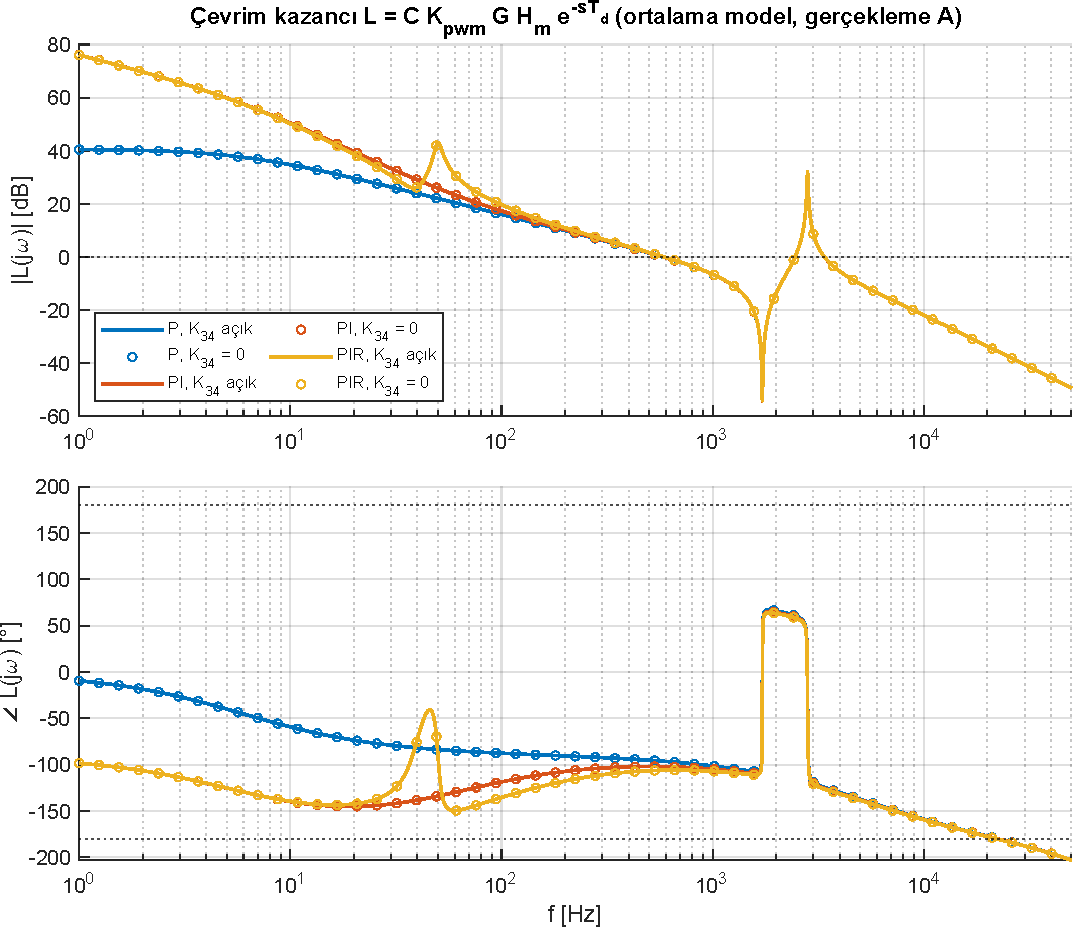
\includegraphics[width=\textwidth,height=0.5\textheight,keepaspectratio]{../tez-matlab-simulink/runs/2026-10-28_kararlilik/frekans/kararlilik_L_bode_K34.pdf}
  \caption{S4 akım çevriminin açık çevrim kazancı $L(j\omega)$, P, PI ve PIR denetleyicileri, gerçekleme (A), \SI{25}{\ampere}; $K_{34}$ açık (çizgi) ve $K_{34}=0$ (işaretçi) eğrileri örtüşür.}
  \label{fig:kararlilik-l-bode}
\end{figure}

\begin{figure}[H]
  \centering
  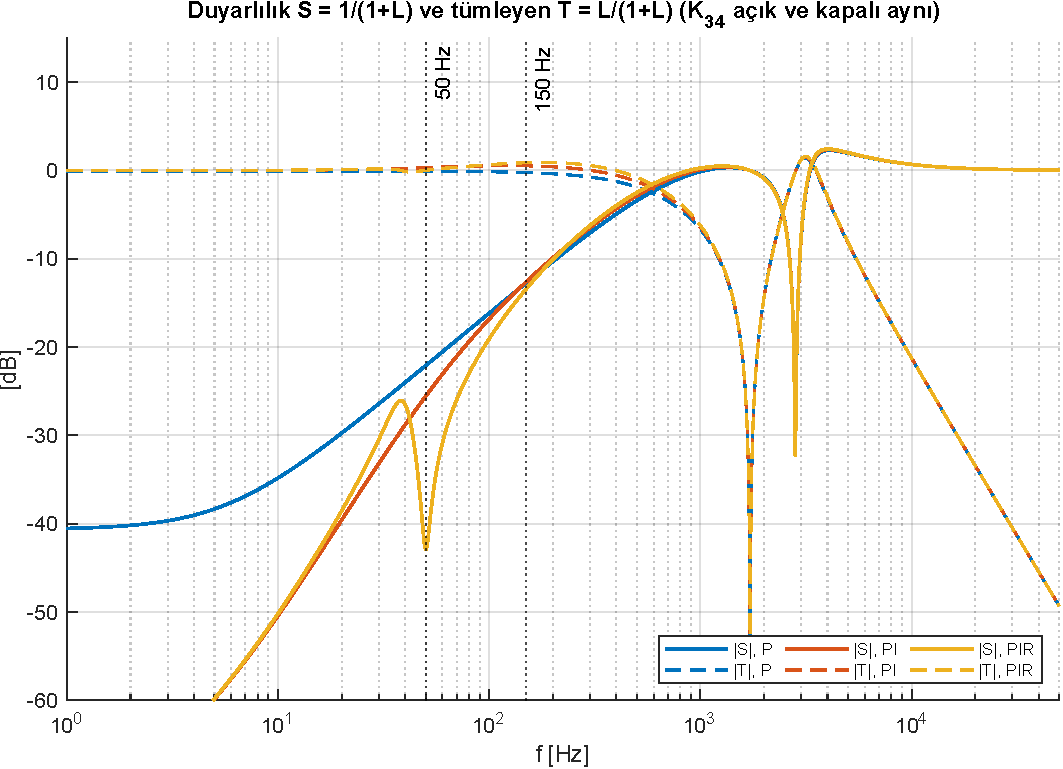
\includegraphics[width=\textwidth,height=0.45\textheight,keepaspectratio]{../tez-matlab-simulink/runs/2026-10-28_kararlilik/frekans/kararlilik_S_T.pdf}
  \caption{S4 akım çevriminin duyarlılık $|S(j\omega)|$ ve tamamlayıcı duyarlılık $|T(j\omega)|$ eğrileri; \SI{50}{\hertz} ve \SI{150}{\hertz} noktaları işaretlidir.}
  \label{fig:kararlilik-s-t}
\end{figure}

Kapalı çevrim kutupları kararlılık hükmünü bağımsız olarak doğrulamaktadır. Gerçekleme (A)'da en az sönümlü kutup çifti P için \SI{3097}{\hertz} ($\zeta=0{,}184$), PI için \SI{3109}{\hertz} ($\zeta=0{,}181$), PIR için \SI{3117}{\hertz} ($\zeta=0{,}179$) çevresindedir. PI'de PI sıfırına yakın \SI{66}{\hertz}'lik gerçel bir kutup, PIR'de ise rezonans teriminden gelen \SI{40.1}{\hertz}, $\zeta=0{,}155$ yavaş bir çift bulunur. Yavaş çiftin yaklaşık \SI{26}{\milli\second} zaman sabiti, PIR benzetimlerinin \SI{0.06}{\second}'de oturmayıp \SI{0.2}{\second} gerektirmesinin nedenidir.

Kararlılık sonucu, ortalama Simulink/Simscape modelinin Simulink Control Design ile doğrusallaştırılmasıyla ayrıca doğrulanmıştır. Ortalama modelde denetleyici alt sistemi, ölçüm süzgeci, doyum, doyum önleme ve ileri besleme blokları anahtarlamalı S4 modelindekilerle aynıdır; köprü, $K_{\mathrm{pwm}}$ kazançlı denetimli gerilim kaynağıyla temsil edilmiştir. Doğrusallaştırılan $L$ ile analitik $L$ arasındaki en büyük göreli fark P, PI ve PIR için sırasıyla $1{,}6\cdot10^{-11}$, $3{,}5\cdot10^{-10}$ ve $6{,}4\cdot10^{-4}$'tür (faz $\leq0{,}04^{\circ}$); $K_{34}$ açık ve kapalı doğrusallaştırmalar arasındaki fark sıfırdır.

\textbf{Sayısal gerçeklemenin kararsızlığı.} Gerçekleme (B)'de ortalama örnekleme, hesaplama ve tutucu gecikmelerinin toplamı iki PWM periyodudur (\SI{200}{\micro\second}) ve rezonansta fazı $-180^{\circ}$'nin altına iter. $L$, $|L|\simeq\SI{30}{\decibel}$ iken negatif gerçel ekseni $-32{,}7$ noktasında keser; Nyquist net kesişimi 1'dir ve \SI{2.72}{\kilo\hertz}'te bir çift kararsız kutup oluşur ($|z|=1{,}175$--$1{,}179$). Periyotta iki güncelleme (B2) de yetmez ($|z|=1{,}085$): gecikme \SI{100}{\micro\second}'ye inse de analog eşdeğerin \SI{44}{\micro\second}'lik gecikme marjının üstündedir. Gecikme taraması aynı sınırı doğrular: PI çevrimi $T_d=\SI{45}{\micro\second}$'de kararlı, \SI{50}{\micro\second}'de kararsızdır. Rezonans frekansı $f_s/6\simeq\SI{1.67}{\kilo\hertz}$'in üstünde olan LCL filtrede $L_1$ akımı geri beslemesi, sayısal gecikmeyle birlikte aktif sönümleme olmadan kararsızdır \citep{Lu2016,Wang2024}. S4, sayısal gerçeklemenin kararsızlığı göz önünde tutularak analog eşdeğer olarak sunulmuştur; sayısal gerçekleme için kapasitör akımı geri beslemesi gibi bir aktif sönümleme yöntemi ya da şebeke akımı geri beslemesi gereklidir. Şekil~\ref{fig:kararlilik-nyquist} iki gerçeklemenin Nyquist eğrilerini $-1$ noktası çevresinde göstermektedir. Gerçekleme (A)'da gecikme 0--\SI{10}{\micro\second} aralığında değiştirildiğinde en küçük faz marjı $56{,}6^{\circ}$'den $44{,}4^{\circ}$'ye iner; kararlılık hükmü değişmez.

\begin{figure}[H]
  \centering
  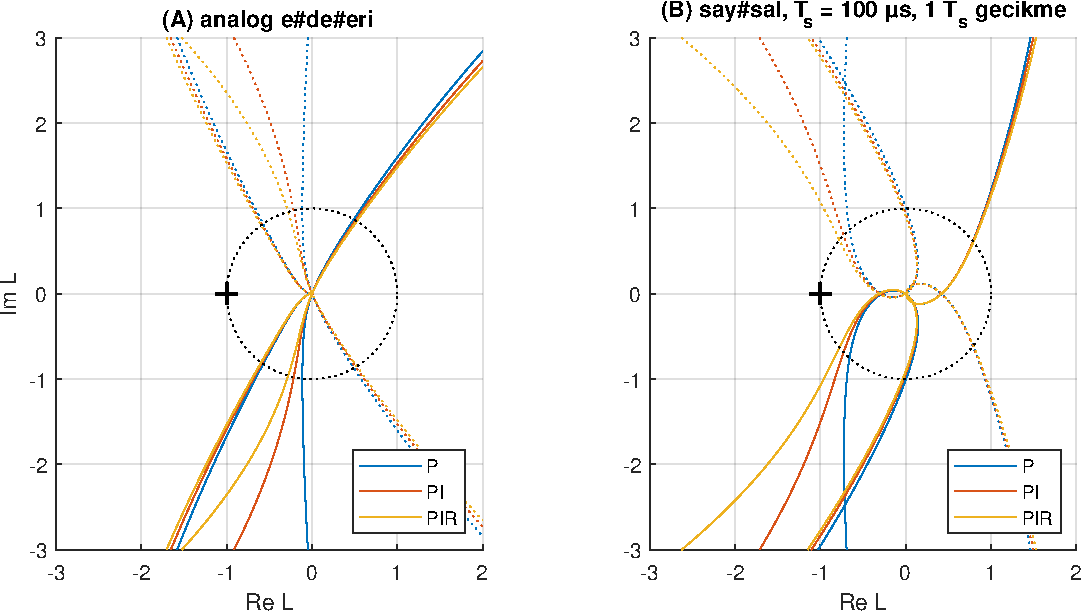
\includegraphics[width=\textwidth,height=0.45\textheight,keepaspectratio]{../tez-matlab-simulink/runs/2026-10-28_kararlilik/frekans/kararlilik_nyquist_A_B.pdf}
  \caption{S4 akım çevriminin Nyquist eğrileri: analog eşdeğer (A) $-1$ noktasını çevrelemez; bir periyot hesaplama gecikmeli sayısal gerçekleme (B) rezonansta negatif gerçel ekseni $-1$'in solunda keser.}
  \label{fig:kararlilik-nyquist}
\end{figure}

\textbf{Şebeke endüktansı duyarlılığı.} $L_2$, şebeke ve varyak endüktansını içerir. Zayıf şebeke ya da uzun hat etkisi için $L_2$'ye 0--\SI{5}{\milli\henry} ek endüktans $L_g$ eklenmiştir (Tablo~\ref{tab:kararlilik-lg}, Şekil~\ref{fig:kararlilik-lg}). Gerçekleme (A) bütün aralıkta kararlıdır; kritik geçişin faz marjı $54^{\circ}$'den $56^{\circ}$'ye hafifçe artar, kazanç marjı değişmez, çünkü yüksek frekansta $L$, $L_1$ ile belirlenir. Bedeli izleme bant genişliğidir: $L_g$ büyüdükçe antirezonans aşağı iner ve birinci geçiş \SI{586}{\hertz}'ten \SI{158}{\hertz}'e düşer. Gerçekleme (B) her $L_g$ değerinde kararsızdır ve kötüleşir.

\begin{table}[H]
  \centering
  \caption{Ek şebeke endüktansının S4 PI çevrimine etkisi.}
  \label{tab:kararlilik-lg}
  \small
  \begin{tabular}{@{}c c c c c c@{}}
    \toprule
    $L_g$ (mH) & $f_{\mathrm{res}}$ / $f_{\mathrm{antirez}}$ (Hz) & 1. geçiş (Hz) & $\mathrm{PM}_{\min}$ ($^{\circ}$) & GM (dB) & (B) $\max|z|$ \\
    \midrule
    0   & 2815 / 1720 & 586 & 54,2 & 35,2 & 1,175 \\
    0,5 & 2635 / 1406 & 450 & 54,9 & 35,2 & 1,215 \\
    1   & 2540 / 1218 & 367 & 55,3 & 35,2 & 1,236 \\
    2   & 2441 / 995  & 271 & 55,7 & 35,2 & 1,257 \\
    5   & 2337 / 704  & 158 & 56,1 & 35,2 & 1,277 \\
    \bottomrule
  \end{tabular}
\end{table}

\begin{figure}[H]
  \centering
  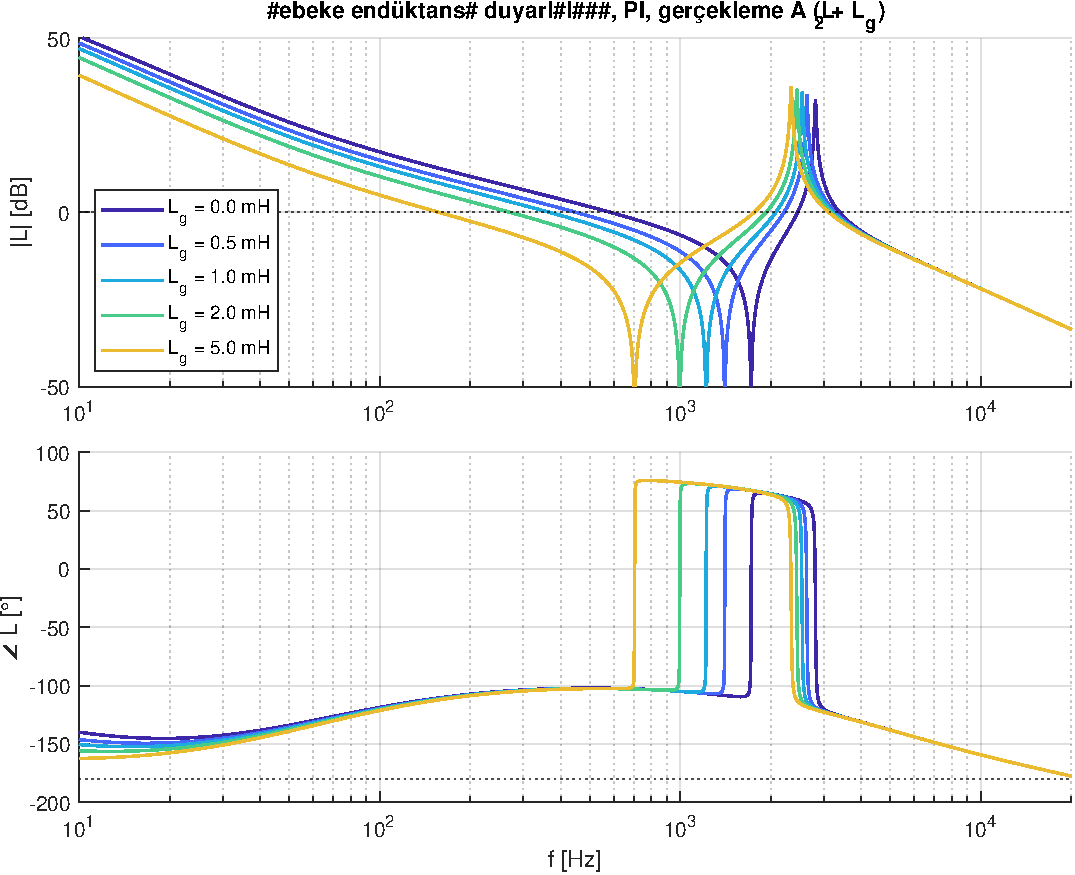
\includegraphics[width=\textwidth,height=0.42\textheight,keepaspectratio]{../tez-matlab-simulink/runs/2026-10-28_kararlilik/frekans/kararlilik_Lg_taramasi.pdf}
  \caption{Ek şebeke endüktansı $L_g=0$--\SI{5}{\milli\henry} için S4 PI çevriminin $L(j\omega)$ eğrileri, gerçekleme (A).}
  \label{fig:kararlilik-lg}
\end{figure}

Köprünün etkin küçük işaret kazancı süreksiz iletimde değişir. PWM kazancı $\lambda K_{\mathrm{pwm}}$ ile ölçeklendiğinde çevrim $\lambda=0{,}05$--50 aralığında kararlı, $\lambda=60$'ta kararsızdır; sınır $+$\SI{35.2}{\decibel} kazanç marjıyla tutarlıdır. Kazanç azalması kararlılığı bozmaz, yalnız birinci geçişi aşağı çeker ($\lambda=0{,}1$'de \SI{79}{\hertz}) ve izleme hatasını büyütür.

\subsection{Zaman alanı: anahtarlamalı modelde doğrulama}

Anahtarlamalı model doğrudan doğrusallaştırılamaz: PWM karşılaştırıcısının ve kip mantığının yerel türevi hemen her yerde sıfırdır ve doğrusallaştırma denetlenen sistemin yolunu keser. Çevrim kazancı, doğrusallaştırma yerine enjeksiyonla ölçülmüştür. Anahtarlamalı S4 modelinin bir ölçüm kopyasında modülasyon toplamına küçük bir işaret $d$ eklenmiştir ($u_x=u_{\mathrm{fb}}+d$); $d=0$ iken model taramadaki modelle matematiksel olarak aynıdır. $d$, her biri 0,015 genlikli üç tonlu (Schroeder fazlı) bir toplamdır; \SI{80}{\milli\second} pencerede tonlar \SI{50}{\hertz} harmoniklerine ve \SI{100}{\hertz} dönüşüm ürünlerine dik seçilmiştir (212,5 / 525 / 1037,5~Hz ve 587,5 / 2025 / 3362,5~Hz). Çevrim kazancı $L=-U_{\mathrm{fb}}/U_x$ olarak kestirilmiştir. Belirsizlik, tona komşu ve ton taşımayan ızgara noktalarındaki $u_x$ düzeyinden, yani anahtarlama ve kip dönüşümü kaynaklı arka plandan hesaplanmıştır. Enjeksiyonlu benzetimlerin temel bileşeni enjeksiyonsuz benzetimlerle aynıdır (PI, \SI{25}{\ampere}: \SI{24.46}{\ampere} ve \SI{24.47}{\ampere}); enjeksiyon çalışma noktasını bozmamıştır.

\begin{table}[H]
  \centering
  \caption{S4 PI çevrim kazancı $L(j\omega)$: analitik gerçekleme (A) ile anahtarlamalı modelde enjeksiyonla ölçülen değerler; hücrelerde $|L|$ (dB) / $\angle L$ ($^{\circ}$).}
  \label{tab:kararlilik-olcum}
  \scriptsize
  \setlength{\tabcolsep}{3pt}
  \begin{tabular}{@{}r c c c c c c@{}}
    \toprule
    $f$ (Hz) & Analitik (A) & \SI{25}{\ampere}, $K_{34}$ açık & \SI{25}{\ampere}, $K_{34}=0$ & \SI{10}{\ampere} & \SI{2.3}{\ampere} & Belirsizlik \\
    \midrule
    212,5  & 9,74 / $-106{,}7^{\circ}$ & 9,90 / $-94{,}4^{\circ}$ & 10,19 / $-90{,}2^{\circ}$ & 8,36 / $-68{,}5^{\circ}$ & $-7{,}25$ / $-25{,}8^{\circ}$ & $\pm1{,}4$~dB / $\pm10^{\circ}$ \\
    525    & 1,11 / $-102{,}2^{\circ}$ & 1,29 / $-94{,}5^{\circ}$ & 1,31 / $-93{,}4^{\circ}$ & 0,66 / $-84{,}7^{\circ}$ & $-8{,}11$ / $-30{,}1^{\circ}$ & $\pm0{,}8$~dB / $\pm6^{\circ}$ \\
    587,5  & $-0{,}03$ / $-102{,}3^{\circ}$ & 0,18 / $-95{,}3^{\circ}$ & 0,32 / $-93{,}8^{\circ}$ & $-0{,}19$ / $-86{,}5^{\circ}$ & -- & $\pm0{,}6$~dB / $\pm4^{\circ}$ \\
    1037,5 & $-7{,}10$ / $-105{,}3^{\circ}$ & $-6{,}05$ / $-98{,}6^{\circ}$ & $-6{,}75$ / $-90{,}4^{\circ}$ & $-7{,}00$ / $-91{,}6^{\circ}$ & $-10{,}05$ / $-48{,}8^{\circ}$ & $\pm1{,}0$~dB / $\pm7^{\circ}$ \\
    2025   & $-12{,}67$ / $+63{,}9^{\circ}$ & $-11{,}00$ / $+60{,}5^{\circ}$ & $-10{,}08$ / $+54{,}4^{\circ}$ & $-10{,}62$ / $+49{,}1^{\circ}$ & -- & $\pm0{,}7$~dB / $\pm5^{\circ}$ \\
    3362,5 & 0,31 / $-125{,}6^{\circ}$ & 0,47 / $-126{,}7^{\circ}$ & 0,59 / $-122{,}5^{\circ}$ & 0,25 / $-114{,}9^{\circ}$ & -- & $\pm0{,}4$~dB / $\pm2{,}5^{\circ}$ \\
    \bottomrule
  \end{tabular}
\end{table}

Tablo~\ref{tab:kararlilik-olcum} ve Şekil~\ref{fig:kararlilik-olcum}, ölçülen ve analitik çevrim kazançlarını karşılaştırmaktadır. Ölçüm yönteminin kendisi iki yoldan denetlenmiştir: ölçülen denetleyici tasarım değerine 0,995--1,004 oranında ve $0{,}6^{\circ}$ içinde, ölçülen pasif ağ $I_{L1}/V_{\mathrm{inv}}$ analitik $G$'ye 0,987--1,028 oranında ve $3{,}4^{\circ}$ içinde eşittir. Ölçülen ve analitik $L$ arasındaki fark, köprünün etkin küçük işaret kazancından gelmektedir. Anma akımında ortalama model kritik bölgeyi doğru vermektedir: \SI{3362.5}{\hertz}'te fark $+$\SI{0.16}{\decibel} ve $-1{,}1^{\circ}$, ölçüm belirsizliği $\pm$\SI{0.4}{\decibel} ve $\pm2{,}5^{\circ}$'dir. Ölçümden kestirilen kritik faz marjı \SI{25}{\ampere}'de $K_{34}$ açıkken yaklaşık $53\pm3^{\circ}$, $K_{34}=0$ iken yaklaşık $57\pm3^{\circ}$, \SI{10}{\ampere}'de yaklaşık $65\pm2^{\circ}$'dir; analitik değer $54{,}2^{\circ}$'dir. \SI{212}{}--\SI{1037}{\hertz} aralığında anahtarlamalı model $7$--$12^{\circ}$ faz öndeliği göstermektedir; faz öndeliği sıfır geçişleri çevresindeki süreksiz iletim ve ölü zaman davranışından gelir ve marjı artırır. $K_{34}$ açık ve kapalı ölçümler arasındaki fark 0,02--\SI{0.9}{\decibel} ve $1$--$8^{\circ}$'dir; fark her noktada iki ölçümün birleşik belirsizliği içinde ya da sınırındadır ve iki benzetimin farklı akımda (\SI{24.5}{\ampere} ve \SI{21.9}{\ampere}) çalışmasından kaynaklanır.

\begin{figure}[H]
  \centering
  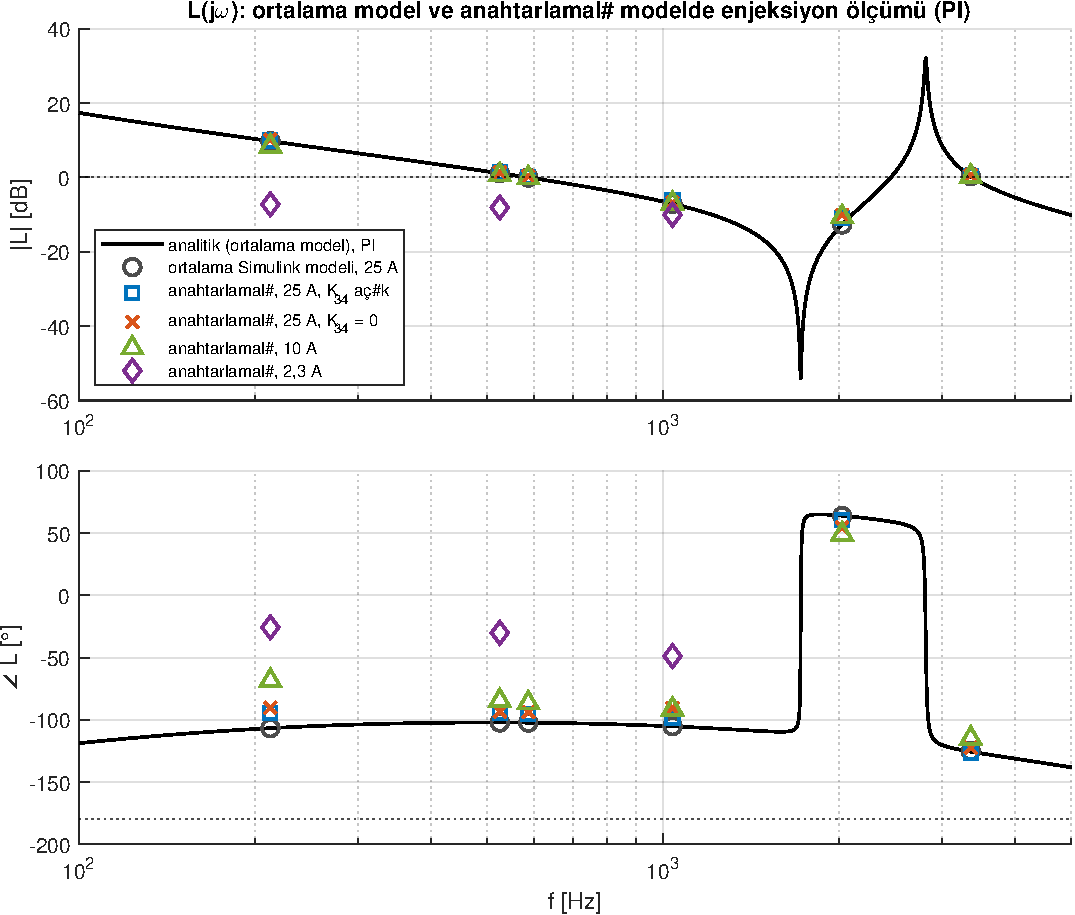
\includegraphics[width=\textwidth,height=0.45\textheight,keepaspectratio]{../tez-matlab-simulink/runs/2026-10-28_kararlilik/karsilastirma/kararlilik_L_olcum_karsilastirma.pdf}
  \caption{S4 PI çevrim kazancı: analitik $L(j\omega)$ eğrisi ile ortalama modelde ve anahtarlamalı modelde enjeksiyonla ölçülen noktalar (\SI{25}{\ampere} $K_{34}$ açık ve kapalı, \SI{10}{\ampere}, \SI{2.3}{\ampere}).}
  \label{fig:kararlilik-olcum}
\end{figure}

Orta ve düşük akımda köprünün etkin kazancı düşer ve faz öndeliği artar. \SI{10}{\ampere}'de etkin kazanç \SI{212}{\hertz}'te tasarım değerinin 0,87 katı ve $+40^{\circ}$ önde, \SI{2.3}{\ampere}'de ise 0,14--0,71 kat ve $+56$--$84^{\circ}$ öndedir. \SI{2.3}{\ampere}'de köprü süreksiz iletimde akım kaynağına yakın davranır: çevrim kazancı \SI{212}{}--\SI{1037}{\hertz} aralığında $-7$ ile \SI{-10}{\decibel} arasında, fazı $-49^{\circ}$'den öndedir; çevrim yavaş ama kararlıdır. Ortalama model düşük akımda izleme başarımını gerçekte olduğundan iyi gösterir; kararlılık sonucu ise korunur, çünkü ölçülen bütün noktalarda faz analitik değerden önde ya da ona eşittir ve köprü kazancının azalması kararlılığı bozmaz.

\textbf{Sin\textsuperscript{3}'ün üçüncü harmonik bulgusu.} Anma akımında $L_1$ akımındaki üçüncü harmoniğin kaynağı Sin\textsuperscript{3} teriminin kendisidir: \SI{25}{\ampere}'de $I_{L1,3}$, $K_{34}$ açıkken \SI{2.13}{\ampere}, $K_{34}=0$ iken \SI{0.43}{\ampere}'dir; THD sırasıyla \%9,4 ve \%5,6'dır. Kalibre $K_{34}$, \SI{2.3}{\ampere}'deki süreksiz iletim bozulmasını kompanze edecek büyüklüktedir; anma akımında bozulma küçük olduğundan terim fazla gelir ve çevrim onu $|S(j2\pi\cdot\SI{150}{\hertz})|=0{,}23$ oranında bastırır ama sıfırlamaz. Temel bileşende ise terim yararlıdır: $K_{34}=0$ iken PI genlik hatası $-$\%2,1'den $-$\%12,3'e çıkar. Kapalı çevrimde ileri besleme genliğinin akım düzeyine göre ayarlanması önerilir; öneri tezde uygulanmamıştır.

\textbf{Basamak yanıtı.} \SI{10}{\ampere}$\rightarrow$\SI{25}{\ampere} basamağı anahtarlamalı ve ortalama modelde $K_{34}$ açık ve kapalı olarak yinelenmiştir (Tablo~\ref{tab:kararlilik-basamak}, Şekil~\ref{fig:kararlilik-basamak}). Geçici bileşen, $i_{L1}(t)-i_{L1}(t+\SI{20}{\milli\second})$ farkı olarak tanımlanmıştır. Dört benzetimde de geçici bileşen aynı biçimde yaklaşık \SI{1}{\milli\second}'de söner; süre \SI{3.1}{\kilo\hertz}, $\zeta=0{,}18$ kutup çiftiyle ve 0,8--\SI{3}{\kilo\hertz} gerçel kutuplarla uyumludur ve ardından \SI{66}{\hertz}'lik PI kipi gelir. Anahtarlamalı modelde $K_{34}$ açık ve kapalı geçici bileşenler arasındaki fark \SI{0.61}{\ampere} RMS'dir (basamak tepesinin \%2,9'u).

\begin{table}[H]
  \centering
  \caption{S4 PI \SI{10}{\ampere}$\rightarrow$\SI{25}{\ampere} basamağında $K_{34}$ açık ve kapalı geçici yanıt.}
  \label{tab:kararlilik-basamak}
  \small
  \begin{tabularx}{\textwidth}{@{}X c c >{\raggedright\arraybackslash}p{0.34\textwidth}@{}}
    \toprule
    Benzetim & Zarf aşımı & Yerleşme (ms) & Ortalama modelden geçici fark (ilk \SI{15}{\milli\second}) \\
    \midrule
    Anahtarlamalı, $K_{34}$ açık & \%0,17 & 0,43 & \SI{0.38}{\ampere} RMS (\%1,8) \\
    Anahtarlamalı, $K_{34}=0$    & $-$\%0,5 & 0,69 & \SI{0.67}{\ampere} RMS (\%3,1) \\
    Ortalama, $K_{34}$ açık      & \%0,0 & 0,41 & -- \\
    Ortalama, $K_{34}=0$         & \%1,5 & 0,66 & -- \\
    \bottomrule
  \end{tabularx}
\end{table}

\begin{figure}[H]
  \centering
  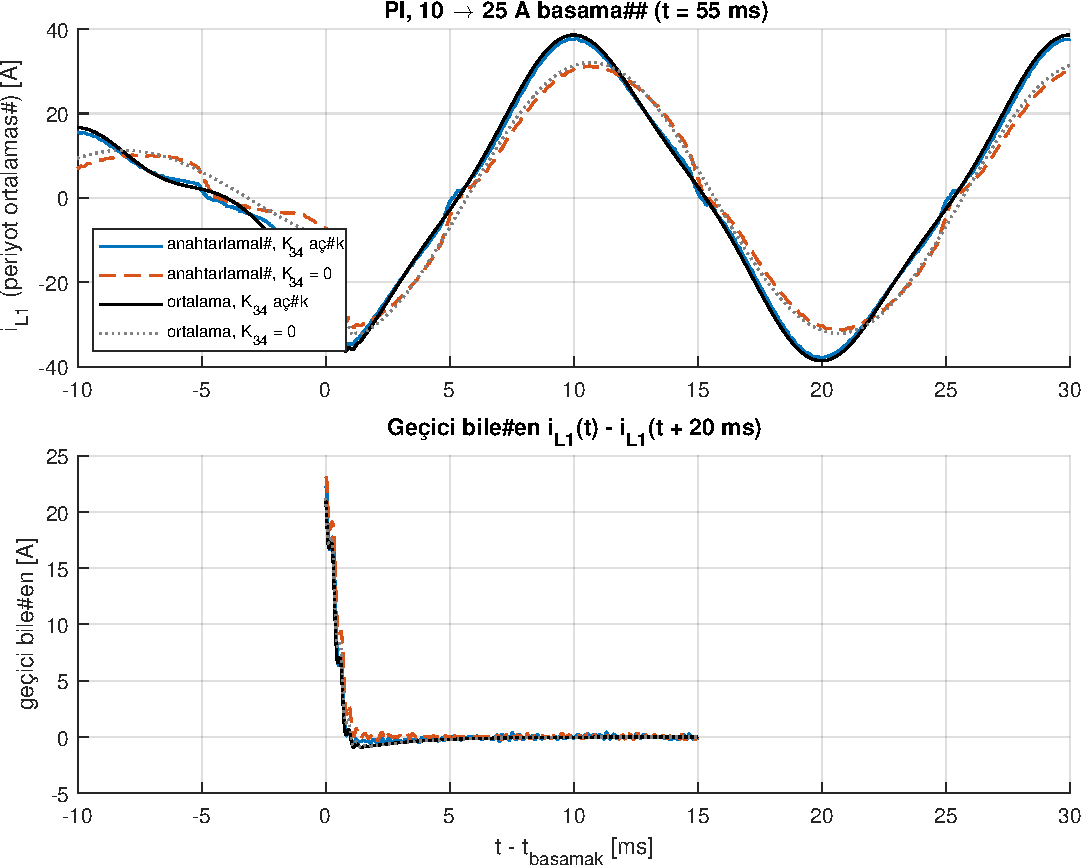
\includegraphics[width=\textwidth,height=0.45\textheight,keepaspectratio]{../tez-matlab-simulink/runs/2026-10-28_kararlilik/karsilastirma/kararlilik_basamak_K34.pdf}
  \caption{S4 PI \SI{10}{\ampere}$\rightarrow$\SI{25}{\ampere} basamağının geçici bileşeni; anahtarlamalı ve ortalama model, $K_{34}$ açık ve kapalı.}
  \label{fig:kararlilik-basamak}
\end{figure}

\subsection{Kararlılık analizinin sınırları}

Ortalama model, anma akımında sürekli iletim bölgesinde kritik frekans aralığını $\pm$\SI{0.2}{\decibel} ve $\pm1^{\circ}$ içinde vermektedir; orta ve düşük akımda köprünün etkin kazancı frekansa bağlı değiştiğinden ortalama model izleme başarımını iyimser gösterir. \SI{2.3}{\ampere}'de enjeksiyon ölçümü \SI{212}{}--\SI{1037}{\hertz} aralığını kapsar; 2--\SI{3.4}{\kilo\hertz} bölgesi ölçülmemiştir. Anahtarlamalı modelde enjeksiyon ölçümü PI denetleyiciyle yapılmıştır; denetlenen sistemin yanıtı ölçüldüğü ve denetleyicinin doğrusal olduğu doğrulandığı için P ve PIR çevrim kazançları ölçülen denetlenen sistem yanıtından yazılabilir. Gecikme $T_d=\SI{2}{\micro\second}$ bir üst sınırdır; analog eşdeğerin kararlılığı 0--\SI{10}{\micro\second} gecikme aralığında doğrulanmış ve gecikme marjı \SI{44}{\micro\second} bulunmuştur. Donanımın örnekleme yapısına ilişkin veri yoktur. Nötr susturmanın periyodik kip değişimi düşük akımda harmonikler arası bağlaşımı belirginleştirebilir; düşük akım için Eşitlik~\eqref{eq:htf-matris-iliskisi} çerçevesinde bir HTF ya da harmonik durum uzayı modeli kurulmamıştır \citep{Liao2022}. Faz payı bara kapasitansıyla \SI{25}{\ampere}'de kararlı durum oluşmadığından kararlılık analizi, S4 anma akımı benzetimlerindeki büyütülmüş bara kapasitansıyla yapılmıştır.

\section{Bölüm Sonucu}

Sin\textsuperscript{3} özdeşliği temel ve üçüncü harmonik bileşenini tek bir anlık terimde birleştirmekte, doğrudan $\sin(3\theta)$ enjeksiyonuyla aynı katsayı anlamını taşımamaktadır. Benzetim modelinde terim birim sinüsün küpü olarak, pozitif işaretle ve normalizasyonsuz biçimde modülasyon toplamına eklenmektedir. DCM/CCM parçalı modeli, nötr susturma sonrasında sinüzoidal görev oranının neden sinüzoidal akım üretmediğini göstermiş; doğru özdeşlikle yapılan analitik tarama, saf sinüs görev oranındaki \%39,96'lık üçüncü harmonik oranını $(D_1,D_3)=(0{,}34,\ 0{,}40)$ adayında \%0,15'e indirmiştir. Analitik adayın üçüncü harmonik katsayısı ($-0{,}10$), anahtarlamalı modelin kalibre katsayısına ($-0{,}096$) yakındır; katsayı seçimi çalışma noktasına bağlıdır.

S4 benzetiminde PI ve PIR akım denetimi \SI{25}{\ampere} anma akımında referansı sırasıyla $-$\%2,1 ve $-$\%1,0 genlik hatasıyla, doyumsuz ve \%8,5--9,2 THD ile izlemektedir; \SI{10}{\ampere}$\rightarrow$\SI{25}{\ampere} basamağında son kararlı zarfa göre aşım \%0,2, yerleşme \SI{0.44}{\milli\second}'dir. Anma akımı sonuçlarının önkoşulu, faz başına modelde DA bara orta noktasını tutabilen bir bara kapasitansıdır. Orta akımda (\SI{10}{\ampere}) nötr susturmanın yarattığı süreksiz iletim THD'yi \%20 düzeyine çıkarmakta ve yöntemin düşük güç kapsamını sınırlamaktadır.

Kararlılık analizi Sin\textsuperscript{3} teriminin bir denetleyici değil, çevrim dışından eklenen bilinen bir giriş olduğunu üç katmanda göstermiştir: karakteristik denklem $1+L(s)=0$ terimi içermez; $L$, $S$ ve $T$, $K_{34}$ açık ve kapalıyken ortalama modelde ve doğrusallaştırmada aynıdır, anahtarlamalı modelde ise farklar ölçüm belirsizliği düzeyindedir; terimin akıma etkisi $S(j\omega)K_{\mathrm{pwm}}G(j\omega)$ ile belirlenir ve \SI{150}{\hertz} bileşeni $|S|=0{,}23$ oranında bastırılır. Analog eşdeğer S4 çevrimi kritik geçişte $54^{\circ}$ faz marjı, $+$\SI{35}{\decibel} kazanç marjı ve \SI{44}{\micro\second} gecikme marjıyla kararlıdır ve 0--\SI{5}{\milli\henry} ek şebeke endüktansında kararlı kalır. Bir periyot gecikmeli sayısal gerçekleme ise aktif sönümleme olmadan kararsızdır; donanım uygulaması için aktif sönümleme gereklidir.

\chapter{DENEYSEL DOĞRULAMA}
\label{chap:deney}

Bölüm~\ref{chap:anahtarlama} ve Bölüm~\ref{chap:sin3} içinde benzetim düzeyinde incelenen klasik anahtarlama, nötr anahtar susturma ve susturma+Sin\textsuperscript{3} yöntemleri, geliştirilen üç fazlı T-tipi prototipin tek faz kolunda, düşük güç koşulunda karşılaştırılmıştır. Bölümde deney düzeneği, güç donanımı, denetim ve ölçüm zinciri testleri yeniden üretecek ayrıntıda tanıtılmakta, deney kayıtları değerlendirilmekte ve benzetim modelinin deney özetine kalibrasyonu (Alt Bölüm~\ref{sec:kalibrasyon}) verilmektedir. Deneyler güvenli laboratuvar koşulunda, yaklaşık \SI{2.3}{\ampere} faz akımındaki düşük güç noktasında yürütülmüştür. Anma gücündeki geri beslemeli (S4) çalışma kalibre benzetim modeliyle, GT-tipi şarj yönü ise Bölüm~\ref{chap:gttipi} içinde benzetim kayıtlarıyla incelenmiştir. Deney kayıtlarındaki metin, tablo ve ekran değerleri birbiriyle tutarlılık bakımından denetlenmiştir.

\textbf{Deneysel veri kümesi.} Deneysel veri kümesi, üç yönteme ait PC yazılımı ekranları, osiloskop ekranları ve her yöntem için bir satırlık deney özet tablosundan oluşmaktadır (Tablo~\ref{tab:gelen-excel-senaryolar}). Ölçüm belirsizliği üretici toleransları ve okuma çözünürlüğünden kestirilmiştir. Benzetim modeli deney özetinin aktif ve reaktif gücüne kalibre edilmiş, diğer büyüklükler bağımsız karşılaştırma olarak raporlanmıştır (Alt Bölüm~\ref{sec:kalibrasyon}). Donanım fotoğrafları, devre kartı çizimleri, osiloskop ve PC yazılımı ekranları deney kayıtlarındaki özgün görüntü dosyalarından alınmış ve özgün çözünürlükleriyle verilmiştir. Bölümdeki sayısal değerler deney özet tablosundan ve ekranlarda yazılı değerlerden okunmuştur; ekran üzerinden yapılan tek ölçüm, Alt Bölüm~\ref{sec:thd-kaynaklar} içindeki faz akımı izlerinin sayısallaştırılmasıdır.

\section{Deney Düzeneği ve Güç Donanımı}

Deney düzeneği, yaklaşık 20--25~kW güç dönüştürme kapasitesi hedeflenerek düşey bir pano üzerine bakır baralarla modüler biçimde kurulmuştur. Akım sensörü boyutlandırma hesabında prototip gücü \SI{20}{\kilo\volt\ampere} olarak verilmiştir. Tezde \SI{20}{\kilo\volt\ampere} anma görünür gücü, \num{20}--\SI{25}{\kilo\watt} ise tasarım güç aralığı olarak kullanılmaktadır (Tablo~\ref{tab:sistem-parametreleri}). Şebeke gerilimi güvenlik amacıyla varyak üzerinden yaklaşık \SI{120}{\volt} ile sınırlandırılmış, deneyler yaklaşık \SI{2.3}{\ampere} faz akımında, düşük güç noktasında yapılmıştır.

Şekil~\ref{fig:deney-duzenegi-genel}; varyak modülü, evirici panosu, bilgisayar ve osiloskopları aynı görünümde vermektedir. Varyak modülünde enerji bağlantıları, şalt ve koruma ekipmanları, akım transformatörleri ve AA enerji analizörü bulunmakta; üç faz bağımsız varyaklarla ayarlanabilmektedir. Düzenekte aşırı akım, kaçak akım, topraklama ve acil durdurma korumaları bulunmaktadır.

\begin{figure}[H]
  \centering
  \includegraphics[width=0.95\textwidth]{deneysel/onceki_tez_sekil_5_1_deney_duzenegi.png}
  \caption{Deney ve ölçme düzeneklerinin genel görünümü.}
  \label{fig:deney-duzenegi-genel}
\end{figure}

Şekil~\ref{fig:deney-evirici-genel}, evirici donanımının önden genel görünümünü sunmaktadır. Üç faza ait güç modülleri, kontrol ve ölçüm kartları, DA bara bağlantıları ve yardımcı beslemeler aynı pano üzerindedir; genel görünüm, numaralı ayrıntıların verildiği Şekil~\ref{fig:deney-donanim-kartlar} için yerleşim bağlamı sağlamaktadır.

\begin{figure}[H]
  \centering
  \includegraphics[width=0.88\textwidth]{deneysel/onceki_tez_sekil_5_2_evirici_donanimi.jpeg}
  \caption{Evirici donanımının genel görünümü.}
  \label{fig:deney-evirici-genel}
\end{figure}

Şekil~\ref{fig:deney-donanim-kartlar} üzerindeki 1--14 numaraları doğrudan Tablo~\ref{tab:deney-alt-birimler} içindeki açıklamalara karşılık gelmektedir.

\begin{figure}[H]
  \centering
  \includegraphics[width=0.72\textwidth]{deneysel/onceki_tez_sekil_5_3_donanim_alt_birimleri.jpeg}
  \caption{Evirici donanımı ve alt birimlerinin numaralı tanıtımı.}
  \label{fig:deney-donanim-kartlar}
\end{figure}

\clearpage
\begin{table}[H]
  \centering
  \caption{Evirici donanımının alt birimleri.}
  \label{tab:deney-alt-birimler}
  \small
  \begin{tabularx}{0.94\textwidth}{X X}
    \toprule
    1. LCL filtrelerin $L_1$ bobinleri & 2. IGBT kapı sürme kartları \\
    3. Nötr IGBT'leri & 4. Yükseltici (boost) diyotları \\
    5. Fonksiyon değiştirme röleleri & 6. Snubber kapasitörleri \\
    7. Kontrol kartı & 8. Tampon (buffer) kartı \\
    9. Ölçme kartı & 10. LCL filtre kapasitörleri \\
    11. Ani akım (inrush) röleleri & 12. Kumanda beslemeleri \\
    13. Şarj fonksiyonu lambası & 14. Deşarj fonksiyonu lambası \\
    \bottomrule
  \end{tabularx}
\end{table}

Şekil~\ref{fig:deney-faz-donanim-1} ve Şekil~\ref{fig:deney-faz-donanim-2}, aynı faz kolunun iki farklı açıdan çekilmiş ayrıntılarını göstermektedir; her iki görseldeki 1--8 numaraları Tablo~\ref{tab:deney-faz-komponentler} ile birlikte okunmalıdır. İki görüntünün ayrı tutulması; boost diyotları, fonksiyon değiştirme röleleri, DA bara ve snubber kapasitörleri, soğutma düzeni, sürücü kartı ve $L_1$ bobininin fiziksel konumunu kaybetmeden izlemeyi sağlamaktadır.

\begin{figure}[H]
  \centering
  \includegraphics[height=0.68\textheight]{deneysel/onceki_tez_sekil_5_4_faz_donanimlari_1.png}
  \caption{Eviricinin bir fazına ait donanımlar, birinci görünüm.}
  \label{fig:deney-faz-donanim-1}
\end{figure}

\begin{figure}[H]
  \centering
  \includegraphics[height=0.68\textheight]{deneysel/onceki_tez_sekil_5_5_faz_donanimlari_2.png}
  \caption{Eviricinin bir fazına ait donanımlar, ikinci görünüm.}
  \label{fig:deney-faz-donanim-2}
\end{figure}

\clearpage
\begin{table}[H]
  \centering
  \caption{Şekil~\ref{fig:deney-faz-donanim-1} ve Şekil~\ref{fig:deney-faz-donanim-2}'deki faz donanımı bileşenleri.}
  \label{tab:deney-faz-komponentler}
  \small
  \begin{tabularx}{0.94\textwidth}{X X}
    \toprule
    1. Boost diyotları ve kondansatörü & 2. Fonksiyon değiştirme röleleri \\
    3. Snubber kondansatörleri & 4. DA bara elektrolitik kondansatörleri \\
    5. IGBT soğutucu & 6. Yüksek devirli soğutma fanı \\
    7. IGBT kapı sürme kartı & 8. LCL filtre $L_1$ bobini \\
    \bottomrule
  \end{tabularx}
\end{table}

Şekil~\ref{fig:deney-giris-devresi}, evirici giriş devresini ve 1--6 ile işaretlenmiş yardımcı donanımları göstermektedir; numaraların karşılığı Tablo~\ref{tab:deney-giris-komponentler} içindedir. Giriş bölümünün ayrı verilmesi; inrush röleleri, sigorta, yardımcı kaynaklar, EMI filtresi, kontrol kartı ve tampon kartının güç katıyla bağlantısını görünür kılmaktadır.

\begin{figure}[H]
  \centering
  \includegraphics[width=0.94\textwidth]{deneysel/onceki_tez_sekil_5_6_giris_devresi.png}
  \caption{Evirici giriş devresinin ayrıntı görünümü.}
  \label{fig:deney-giris-devresi}
\end{figure}

\clearpage
\begin{table}[H]
  \centering
  \caption{Evirici giriş kısmına ait bileşenler.}
  \label{tab:deney-giris-komponentler}
  \small
  \begin{tabularx}{0.94\textwidth}{X X}
    \toprule
    1. Ani akım (inrush) röleleri & 2. Evirici açma kapama sigortası \\
    3. 12 V--24 V güç kaynakları & 4. EMI filtre \\
    5. Kontrol kartı & 6. Tampon (buffer) kartı \\
    \bottomrule
  \end{tabularx}
\end{table}

\section{Kontrol Kartı, Tampon Kartı ve Kapı Sürücüsü}

Şekil~\ref{fig:deney-kontrol-buffer}, kontrol ve tampon kartlarını numaralı işlevleriyle göstermektedir. Kontrol kartında RS485 haberleşme birimi, optoizole giriş/çıkışlar, DA bara ve akım ölçüm dönüştürme devreleri, PIC32MK ailesi mikrodenetleyici, lineer regülatörler ve röle/fan çıkış katları bulunmaktadır. Tampon kartı, mikrodenetleyicinin \SI{3.3}{\volt} tek uçlu (single-ended) PWM işaretlerini diferansiyel sinyal çiftlerine dönüştürmek ve uzun ekranlı kablolarda ortak-mod gürültü etkisini azaltmak amacıyla kullanılmıştır. Fotoğraftaki numaralar sırasıyla aşağıdaki işlevleri gösterir: (1) RS485 haberleşme; (2)--(3) optoizole giriş ve çıkışlar; (4) diferansiyel DA bara gerilimini tek uçlu biçime dönüştüren ölçüm katı; (5) ölçüm, haberleşme ve kontrol algoritmalarını yürüten PIC32MK mikrodenetleyici; (6) akım ölçüm dönüştürme katı; (7) \SI{5}{\volt} lineer regülatörler; (8) röle ve fanlar için MOSFET güç çıkışları; (9) \SI{9}{\volt} anahtarlamalı regülatör; (10) PWM tampon kartının \SI{9}{\volt} beslemesi; (11) tek uçlu PWM işaretlerini diferansiyel çiftlere dönüştüren kat.

\begin{figure}[H]
  \centering
  \includegraphics[width=0.90\textwidth]{deneysel/onceki_tez_sekil_5_7_kontrol_buffer.png}
  \caption{Kontrol kartı ve tampon kartının numaralı görünümü.}
  \label{fig:deney-kontrol-buffer}
\end{figure}

PWM1--PWM6 kanallarının yüksek ve alçak işaretleri tampon kartında diferansiyel çiftlere dönüştürülmekte; yaklaşık \SI{12}{\volt} genlikte, tek yönlü iletim amacıyla H-köprü tabanlı bir sürme çözümü kullanılmaktadır. PWM zamanlayıcısındaki ölü zaman tasarım değeri \SI{1}{\micro\second}'dir (Tablo~\ref{tab:sistem-parametreleri}).

Şekil~\ref{fig:deney-igbt-surucu}, ADuM4135 tabanlı IGBT kapı sürme kartını göstermektedir. Diferansiyel giriş, desatürasyon koruması, aktif Miller kenetleme ve düşük gerilim kilitleme özellikleri sürücü seçiminin gerekçeleridir: diferansiyel giriş uzun PWM hatlarındaki ortak-mod gürültüsüne bağışıklık sağlar; desatürasyon koruması aşırı akımda IGBT komutunu donanımsal olarak keser; aktif Miller kenetleme yüksek frekanslı anahtarlamada hatalı iletime geçme (false turn-on) riskini azaltır. Bütün sürücülerden gelen FAULT çıkışları kontrol kartında toplanmakta ve ortak RESET işareti sürücülere paralel dağıtılmaktadır. Sonuç olarak donanım koruması ile denetim yazılımı arasında bir hata yönetim zinciri oluşmaktadır.

\begin{figure}[H]
  \centering
  \includegraphics[height=0.64\textheight]{deneysel/onceki_tez_sekil_5_8_igbt_surucu.jpeg}
  \caption{IGBT kapı sürme devresi.}
  \label{fig:deney-igbt-surucu}
\end{figure}

\clearpage
\section{Gerilim ve Akım Ölçme Devreleri}

Faz--nötr gerilimleri ile pozitif ve negatif DA bara gerilimleri, AMC1200 tabanlı izole ölçüm devreleriyle alınmaktadır; ölçüm kartının ofset, ADC aralığı ve DA bara ölçüm aralığı Tablo~\ref{tab:sistem-parametreleri} içindedir. AMC1200'ün gerilim kazancı 8 olduğundan girişte izin verilen en yüksek genlik \SI{162.5}{\milli\volt} olarak hesaplanmış; faz ve DA bara ölçümleri için ayrı gerilim bölücüler kullanılmıştır. Faz ölçüm sınırı anlık yaklaşık \SI{387}{\volt}'tur.

Mikrodenetleyicideki yedi ADC kanalının üçü faz--nötr gerilimlerine, ikisi pozitif ve negatif DA bara gerilimlerine ayrılmıştır. Faz ölçümleri AMC1200 çıkışlarından ekranlı kabloyla diferansiyel olarak taşınmış ve RC örtüşme önleme (anti-aliasing) filtrelerinden geçirilmiştir. DA bara kanallarında diferansiyel işaretler enstrümantasyon yükselteciyle işlenip \SI{1.3}{\volt} ofset eklenerek tek uçlu biçime dönüştürülmektedir. 12 bit ADC gösterimi, diferansiyel sayısal aralığı yaklaşık $-2047$ ile $+2048$ arasında tanımlamaktadır.

Dört telli T-tipi yapıda nötr noktasının kayması iki DA bara kondansatörünün gerilimlerini eşitsizleştirebileceğinden pozitif ve negatif bara kanalları sürekli izlenmekte; eşik aşımında mikrodenetleyici FAULT üretip PWM çıkışlarını kesmektedir. AMC1200 giriş beslemesi RFM-0505S izole dönüştürücü ile sağlanmış; dönüştürücü çıkışındaki regülasyon zayıflığını azaltmak için TCR2EF250 düşük gerilim düşümlü regülatör kullanılmıştır. Ölçüm zinciri, ölçeklemenin yanında izolasyon ve nötr nokta koruması görevlerini de üstlenmektedir.

Akım ölçümünde HLSR 20-P/SP33 Hall etkili sensör kullanılmıştır. Sensör kazancı ve ölçülebilir simetrik tepe akımı Tablo~\ref{tab:sistem-parametreleri} içindedir; tepe sınırın RMS karşılığı yaklaşık \SI{39.9}{\ampere}'dir. Faz başına akım tasarım değeri ve yüzde 20 paylı üst sınırı aynı tabloda verilmiştir. Hesaplar nominal direnç değerlerine dayanmaktadır.

Ani faz ve kondansatör akımlarının sınırlandırılması amacıyla kullanılan pencere karşılaştırıcı devre Şekil~\ref{fig:deney-pencere-karsilastirici} üzerinde verilmiştir. Devrede üst eşik \SI{2.0}{\volt}, alt eşik \SI{0.6}{\volt} olarak, sensör referansına simetrik ayarlanmıştır. Eşiklerin referanstan uzaklığı, sensör kazancıyla Tablo~\ref{tab:sistem-parametreleri} içindeki aşırı akım eşiğine karşılık gelmektedir. Eşik dışına çıkıldığında FAULT işareti kontrol kartında harici kesme oluşturarak PWM çıkışlarını kesmektedir.

\begin{figure}[H]
  \centering
  \includegraphics[width=0.96\textwidth]{deneysel/onceki_tez_sekil_5_9_pencere_karsilastirici.jpeg}
  \caption{Pencere karşılaştırıcı devresi.}
  \label{fig:deney-pencere-karsilastirici}
\end{figure}

Şekil~\ref{fig:deney-pencere-dalga}, harici bir deneme kartının DAC çıkışıyla uygulanan giriş işareti ve pencere karşılaştırıcının FAULT çıkışını göstermektedir. İmleç seviyeleri \SI{2.0}{\volt} ve \SI{0.6}{\volt} olarak ayarlanmış; giriş sınırların dışına çıktığında ikinci kanal işaretinin lojik sıfıra indiği gözlenmiştir. Kayıt, koruma mantığının işlevsel örneğidir; gecikme süresi ve gerçek kısa devre kesme enerjisi aynı görüntüden çıkarılamaz.

\begin{figure}[H]
  \centering
  \includegraphics[width=0.88\textwidth]{deneysel/onceki_tez_sekil_5_10_pencere_dalga.jpeg}
  \caption{Pencere karşılaştırıcı giriş ve çıkış gerilim dalga şekilleri.}
  \label{fig:deney-pencere-dalga}
\end{figure}

Şekil~\ref{fig:deney-olcum-karti}; HLSR akım sensörleri, AMC1200 izole ölçüm kanalları ve akım probu bağlantı iletkenlerini içeren ölçüm kartını göstermektedir. Kart üzerindeki \SI{4}{\milli\metre\squared} kesitli ters-U biçimli iletkenler; faz başına $L_1$ akımı, kondansatör akımı ve faz akımının ayrı ayrı osiloskop probuyla ölçülmesini sağlamaktadır. TLV431 referansları ve MC33269 regülatörleri ölçüm beslemesi ile \SI{1.3}{\volt} ofset üretiminde kullanılmıştır.

\begin{figure}[H]
  \centering
  \includegraphics[width=0.96\textwidth]{deneysel/onceki_tez_sekil_5_11_olcum_karti.jpeg}
  \caption{Ölçüm kartı.}
  \label{fig:deney-olcum-karti}
\end{figure}

\section{DA ve AA Güç Analizörleri}

DA bara gerilimi, akımı ve gücü Accuenergy AcuDC240 analizörüyle ölçülmüştür; üretici akım ve gerilim için yüzde 0,2, güç ve enerji için yüzde 0,5 hata toleransı bildirmektedir. Şekil~\ref{fig:deney-acudc240}(a) cihazın pano üzerindeki konumunu, Şekil~\ref{fig:deney-acudc240}(b) üretici dokümanındaki şönt bağlantısını göstermektedir.

\begin{figure}[H]
  \centering
  \begin{subfigure}[t]{0.46\textwidth}
    \centering
    \includegraphics[width=\linewidth]{deneysel/onceki_tez_sekil_5_12a_acudc240.jpeg}
    \caption{Evirici donanımı üzerindeki AcuDC240.}
  \end{subfigure}\hfill
  \begin{subfigure}[t]{0.50\textwidth}
    \centering
    \includegraphics[width=\linewidth]{deneysel/onceki_tez_sekil_5_12b_acudc240_baglanti.jpeg}
    \caption{DA analizörü ve şönt bağlantı şekli.}
  \end{subfigure}
  \caption{AcuDC240 DA bara analizörü ve bağlantısı.}
  \label{fig:deney-acudc240}
\end{figure}

Prototipte şönt direnci DA baranın negatif terminaline bağlanarak alçak-taraf akım ölçümü yapılmıştır. Şekil~\ref{fig:deney-sont-baglanti}, \SI{20}{\ampere}/\SI{60}{\milli\volt} şönt direncin fiziksel bağlantısını göstermektedir. Şöntün ölçüm uçları koaksiyel ve ekranlı kabloyla analizöre taşınmış; DA gerilim girişinde yüksek izolasyon dayanımlı kablo kullanılmıştır.

\begin{figure}[H]
  \centering
  \includegraphics[width=0.94\textwidth]{deneysel/onceki_tez_sekil_5_13_sont_baglanti.jpeg}
  \caption{\SI{20}{\ampere}--\SI{60}{\milli\volt} şönt direnç bağlantısı.}
  \label{fig:deney-sont-baglanti}
\end{figure}

AA tarafta Entes EMK-01 analizörü ve 50/5 oranlı, \SI{5}{\volt\ampere}, Class~0.1 akım transformatörleri kullanılmıştır. Akım transformatörünün IEC~61869-2'ye göre yapılan kalibrasyon ölçümü EK A'da verilmiştir; deney akımının bulunduğu anma akımının \%5'i bölgesinde oran hatası $-$\%0,046, faz hatası 2,8~dakikadır ve AA güç ölçümünün belirsizliğinde ihmal edilebilir düzeydedir. Üç faz ve nötr hattı için dört akım transformatörü bağlanmış; faz--nötr gerilimleri, faz/nötr akımları, aktif ve reaktif güç ile toplam THD değerleri Modbus RTU üzerinden okunmuştur. Şekil~\ref{fig:deney-emk01}(a) analizörü, Şekil~\ref{fig:deney-emk01}(b) üreticinin bağlantı düzenini vermektedir.

\begin{figure}[H]
  \centering
  \begin{subfigure}[t]{0.43\textwidth}
    \centering
    \includegraphics[width=\linewidth]{deneysel/onceki_tez_sekil_5_14a_emk01.jpeg}
    \caption{EMK-01 AA analizörü.}
  \end{subfigure}\hfill
  \begin{subfigure}[t]{0.53\textwidth}
    \centering
    \includegraphics[width=\linewidth]{deneysel/onceki_tez_sekil_5_14b_emk01_baglanti.png}
    \caption{Üretici tarafından önerilen bağlantı şekli.}
  \end{subfigure}
  \caption{EMK-01 AA analizörü ve bağlantısı.}
  \label{fig:deney-emk01}
\end{figure}

\section{PC Ana Kumanda Yazılımı ve Veri Toplama}

PC ana kumanda yazılımı; EMK-01, AcuDC240 ve kontrol kartından RS485/Modbus RTU üzerinden veri almak, anlık değerleri grafikleştirmek ve verim hesabına temel oluşturmak amacıyla geliştirilmiştir. Şekil~\ref{fig:deney-pc-arayuzu} yazılımın arayüzünü göstermektedir. Bir veri çevrimi yaklaşık \SI{1}{\second} sürmektedir. Her çevrimde önce DA analizörü, en fazla yaklaşık \SI{50}{\milli\second} sonra AA analizörü okunmaktadır. Kayıt yapısı kararlı durum eğilimlerini izlemek ve verimi hesaplamak için kullanılmıştır.

Haberleşme hızı cihazların izin verdiği en yüksek değer olan 38400 baud seçilmiş; veri sırası DA analizörü, AA analizörü ve kontrol kartı biçiminde kurulmuştur. Yazılımın karşılaştırma seti verim, THD, güç faktörü, faz akımı, faz--nötr gerilimi ve DA bara geriliminden oluşmaktadır. Osiloskop kanal adlarında ``kontrolör çıkışı'' ifadesi geçmektedir. Senaryo tanımlarında S1--S3 açık çevrim modülasyonla çalışır ve akım geri beslemesi yalnız S4'te bulunur (Alt Bölüm~\ref{sec:s4-kapali-cevrim}); kanal adındaki ifade, benzetim modelinin yapısına göre modülasyon komutu olarak okunmuştur.

\begin{figure}[H]
  \centering
  \includegraphics[width=0.98\textwidth]{deneysel/onceki_tez_sekil_5_15_pc_arayuzu.png}
  \caption{Haberleşme sistemi arayüzü.}
  \label{fig:deney-pc-arayuzu}
\end{figure}

Ortak hedef çalışma koşulu olarak DA bara gerilimi yaklaşık \SI{400}{\volt}, faz--nötr gerilimi yaklaşık \SI{130}{\volt}, faz akımı yaklaşık \SI{2.3}{\ampere} ve birim güç faktörüne yakın işletim tanımlanmıştır. Üç deneyde gerçekleşen DA bara gerilimleri (\num{431.5}, \num{395.0} ve \SI{427.5}{\volt}) ve şebeke gerilimleri (\num{119.8}, \num{121.0} ve \SI{124.3}{\volt}) birbirinden farklıdır (Tablo~\ref{tab:gelen-excel-senaryolar}). Her benzetim kendi deneyinin DA bara ve şebeke gerilimiyle yapılmıştır. Verim ve THD, Eşitlik~\eqref{eq:verim-tanimi} ve Eşitlik~\eqref{eq:thd-rmse-tanimlari} ile hesaplanmıştır.

\section{Klasik Anahtarlama Modu Deney Kayıtları}

Klasik yöntemde bütün anahtarlar tamamlayıcı sürülmekte ve düşük akımda senkron-buck benzeri ters akım yolu açık kalmaktadır. Deney özeti yüzde 92,5 verim, yüzde 15 faz akımı THD'si, yaklaşık \SI{2.3}{\ampere} faz akımı, \SI{120}{\volt} faz--nötr gerilimi ve \SI{430}{\volt} DA bara gerilimi bildirmektedir.

Şekil~\ref{fig:deney-klasik-pc}, PC yazılımında klasik anahtarlama sırasında elde edilen grafiklerin tamamını göstermektedir; AA/DA analizör değerleri ile güç ve THD eğilimleri aynı arayüzde izlenmektedir. THDi eğrisi yaklaşık 100 saniyelik kayıt boyunca \%5--22 arasında dalgalanmaktadır; özetteki \%15 kaydın ortalama düzeyini, ekrandaki \%11,1 ise tek bir anlık okumayı göstermektedir.

\begin{figure}[H]
  \centering
  \includegraphics[width=0.98\textwidth]{deneysel/onceki_tez_sekil_5_16_klasik_pc.jpeg}
  \caption{Klasik anahtarlama sırasında PC yazılımında alınan grafikler.}
  \label{fig:deney-klasik-pc}
\end{figure}

Şekil~\ref{fig:deney-klasik-l1} üzerinde yukarıdan aşağıya kontrol işareti, şebeke gerilimi, işlemciden alınan ortalama endüktör akımı ve akım probuyla ölçülen $L_1$ akımı bulunmaktadır. Kayıt, anahtarlama dalgalanmasını ve akımın sıfır çevresindeki davranışını doğrudan göstermektedir.

\begin{figure}[H]
  \centering
  \includegraphics[width=0.94\textwidth]{deneysel/onceki_tez_sekil_5_17_klasik_l1.png}
  \caption{Klasik yöntemde kontrol işareti, şebeke gerilimi, ortalama endüktör akımı ve $L_1$ akımı.}
  \label{fig:deney-klasik-l1}
\end{figure}

Şekil~\ref{fig:deney-klasik-faz} üzerinde ilk üç kanal korunmuş, dördüncü kanalda faz akımı verilmiştir. $L_1$ akımı ile faz akımının ayrı kayıtlarda sunulması, filtre ve şebeke tarafındaki dalga biçimlerinin aynı fiziksel büyüklük olarak yorumlanmasını önlemektedir. Faz akımının tepesi yuvarlaktır ve tepeyi bir kambur izlemektedir; izin sayısallaştırılmasıyla elde edilen THD yaklaşık \%21'dir (Alt Bölüm~\ref{sec:thd-kaynaklar}).

\begin{figure}[H]
  \centering
  \includegraphics[width=0.94\textwidth]{deneysel/onceki_tez_sekil_5_18_klasik_faz.png}
  \caption{Klasik yöntemde kontrol işareti, şebeke gerilimi, ortalama endüktör akımı ve faz akımı.}
  \label{fig:deney-klasik-faz}
\end{figure}

\section{Nötr Anahtar Susturma Modu Deney Kayıtları}

Nötr anahtar susturma yönteminde ilgili yarım periyotta ters akım yolu kesilmekte, düşük görev oranında kesintili iletim ve üçüncü harmonik ağırlıklı akım zarfı ortaya çıkmaktadır. Deney özeti yüzde 94,2 verim, yüzde 47 faz akımı THD'si, yaklaşık \SI{2.3}{\ampere} faz akımı, \SI{120}{\volt} faz--nötr gerilimi ve \SI{395}{\volt} DA bara gerilimi vermektedir.

\begin{figure}[H]
  \centering
  \includegraphics[width=0.98\textwidth]{deneysel/onceki_tez_sekil_5_19_susturma_pc.jpeg}
  \caption{Nötr anahtar susturma modunda PC yazılımında elde edilen grafikler.}
  \label{fig:deney-susturma-pc}
\end{figure}

Şekil~\ref{fig:deney-susturma-l1}, anahtarlamalı endüktör akımının sıfır çevresinde kesildiği aralıkları göstermektedir. Gözlenen zarf, Bölüm~\ref{chap:anahtarlama} içindeki kalibre S2 benzetimi ve üçüncü harmonik mekanizmasıyla nitel olarak uyumludur.

\begin{figure}[H]
  \centering
  \includegraphics[width=0.94\textwidth]{deneysel/onceki_tez_sekil_5_20_susturma_l1.png}
  \caption{Susturma yönteminde kontrol işareti, şebeke gerilimi, ortalama endüktör akımı ve $L_1$ akımı.}
  \label{fig:deney-susturma-l1}
\end{figure}

Şekil~\ref{fig:deney-susturma-faz}, aynı yöntemin faz akımındaki belirgin biçim bozulmasını göstermektedir.

\begin{figure}[H]
  \centering
  \includegraphics[width=0.94\textwidth]{deneysel/onceki_tez_sekil_5_21_susturma_faz.png}
  \caption{Susturma yönteminde kontrol işareti, şebeke gerilimi, ortalama endüktör akımı ve faz akımı.}
  \label{fig:deney-susturma-faz}
\end{figure}

\section{Susturma ve Sin\texorpdfstring{\textsuperscript{3}}{3} Modu Deney Kayıtları}

Üçüncü yöntemde nötr anahtar susturma korunmuş ve akım zarfındaki harmonik bozulmayı azaltmak amacıyla Sin\textsuperscript{3} tabanlı terim eklenmiştir. Deney özeti yüzde 94,5 verim, yüzde 14 faz akımı THD'si, yaklaşık \SI{2.3}{\ampere} faz akımı, \SI{124}{\volt} faz--nötr gerilimi ve \SI{427}{\volt} DA bara gerilimi bildirmektedir. Benzetim modelinde terim, deneydeki uygulamaya karşılık gelecek biçimde $K_{33}\sin^3\theta$ olarak tanımlanmıştır (Bölüm~\ref{chap:sin3}).

\begin{figure}[H]
  \centering
  \includegraphics[width=0.98\textwidth]{deneysel/onceki_tez_sekil_5_22_sin3_pc.jpeg}
  \caption{Sin\textsuperscript{3} uygulanmış susturma modunda PC yazılımında alınan grafikler.}
  \label{fig:deney-sin3-pc}
\end{figure}

Şekil~\ref{fig:deney-sin3-l1}, susturma deneyine göre daha düzenli bir $L_1$ akım zarfı göstermektedir; nitel iyileşme, bildirilen THD azalmasıyla uyumludur.

\begin{figure}[H]
  \centering
  \includegraphics[width=0.94\textwidth]{deneysel/onceki_tez_sekil_5_23_sin3_l1.png}
  \caption{Sin\textsuperscript{3} uygulanmış yöntemde kontrol işareti, şebeke gerilimi, ortalama endüktör akımı ve $L_1$ akımı.}
  \label{fig:deney-sin3-l1}
\end{figure}

Şekil~\ref{fig:deney-sin3-faz}, faz akımındaki zarfın susturma yöntemine göre düzeldiğini göstermektedir.

\begin{figure}[H]
  \centering
  \includegraphics[width=0.94\textwidth]{deneysel/onceki_tez_sekil_5_24_sin3_faz.png}
  \caption{Sin\textsuperscript{3} uygulanmış yöntemde kontrol işareti, şebeke gerilimi, ortalama endüktör akımı ve faz akımı.}
  \label{fig:deney-sin3-faz}
\end{figure}

\section{Deney Sonuçlarının Değerlendirilmesi}

Üç yöntemin deneysel ve kalibre benzetim verim ve faz akımı THD değerleri Tablo~\ref{tab:deney-dusuk-guc-ozeti} üzerindedir. AA analizörü şebeke tarafındaki faz akımını ölçtüğünden tabloda yalnız faz akımı THD'si yer almaktadır. Kalibrasyon yöntemi ve bağımsız doğrulama ölçütleri Alt Bölüm~\ref{sec:kalibrasyon} altında ayrıca verilmektedir.

\begin{table}[H]
  \centering
  \caption{Üç yöntemin deney özeti ve kalibre benzetimdeki verim ve faz akımı THD değerleri.}
  \label{tab:deney-dusuk-guc-ozeti}
  \footnotesize
  \begin{tabularx}{\textwidth}{X *{4}{>{\centering\arraybackslash}p{0.13\textwidth}}}
    \toprule
    & \multicolumn{2}{c}{Deney} & \multicolumn{2}{c}{Kalibre benzetim} \\
    \cmidrule(lr){2-3}\cmidrule(lr){4-5}
    Yöntem & Verim & THD$_{i,\mathrm{faz}}$ & Verim & THD$_{i,\mathrm{faz}}$ \\
    \midrule
    Klasik tamamlayıcı anahtarlama & \%92,50 & \%15 & \%91,15 & \%39,5 \\
    Nötr anahtar susturma & \%94,20 & \%47 & \%93,93 & \%56,7 \\
    Susturma + Sin\textsuperscript{3} & \%94,50 & \%14 & \%94,25 & \%14,8 \\
    \bottomrule
  \end{tabularx}
\end{table}

Deneyde susturma verimi 1,7 puan artırırken THD'yi \%47'ye çıkarmıştır. Sin\textsuperscript{3} terimi ise verimi \%94,5 düzeyinde korurken THD'yi \%47'den \%14'e, klasik anahtarlama düzeyine indirmiştir. Kalibre benzetim, verim ve THD sıralamasını deneyle aynı vermektedir.

Deney düzeneğindeki güç, ölçüm ve veri toplama akışı Şekil~\ref{fig:deney-olcum-zinciri} üzerinde özetlenmiştir.

\begin{figure}[H]
  \centering
  \begin{tikzpicture}[
    node distance=8mm and 10mm,
    block/.style={draw=blue!55!black,fill=blue!7,rounded corners,align=center,minimum height=10mm,text width=28mm,font=\small},
    meas/.style={draw=green!50!black,fill=green!8,rounded corners,align=center,minimum height=10mm,text width=28mm,font=\small},
    data/.style={draw=orange!70!black,fill=orange!10,rounded corners,align=center,minimum height=10mm,text width=30mm,font=\small},
    arr/.style={-{Latex[length=2.5mm]},thick}
  ]
    \node[block] (dc) {DA bara\\AcuDC240 + şönt};
    \node[block,right=of dc] (inv) {T-tipi evirici\\LCL filtre};
    \node[block,right=of inv] (grid) {Varyak ve\\AA şebeke};
    \draw[arr] (dc) -- node[above,font=\scriptsize] {$P_{\mathrm{dc}}$} (inv);
    \draw[arr] (inv) -- node[above,font=\scriptsize] {$v_g,i_g$} (grid);
    \node[meas,below=of inv] (scope) {Osiloskop\\$i_{L1}$, $i_g$, $v_g$, DAC};
    \node[meas,below=of grid] (ac) {EMK-01 + CT\\$P_{\mathrm{ac}}$, THD, PF};
    \node[meas,below=of dc] (ctrl) {Kontrol/ölçüm kartı\\ADC, PWM, FAULT};
    \draw[arr] (inv) -- (scope);
    \draw[arr] (grid) -- (ac);
    \draw[arr] (inv) -- (ctrl);
    \node[data,below=15mm of scope] (pc) {PC ana kumanda yazılımı\\RS485/Modbus RTU};
    \draw[arr] (ctrl) -- (pc);
    \draw[arr] (ac) -- (pc);
    \draw[arr] (dc) |- (pc);
    \draw[arr,dashed] (scope) -- node[right,font=\scriptsize] {ekran kaydı} (pc);
  \end{tikzpicture}
  \caption{Deney düzeneğindeki güç, ölçüm ve veri toplama akışı.}
  \label{fig:deney-olcum-zinciri}
\end{figure}

Tablo~\ref{tab:olcum-cihazlari}, kullanılan cihaz ve sensörleri bildirilen özellikleri ve doğruluk bilgisinin kaynağıyla birlikte toplamaktadır. AcuDC240 için hesaplarda veri sayfasındaki yüzde hata değerleri kullanılmıştır.

Üç yöntemin çalışma koşulları Tablo~\ref{tab:deney-kosullari} üzerinde karşılaştırılmıştır.

Deney özet değerleri ile PC ekranlarında görünen anlık değerler arasındaki farklar Tablo~\ref{tab:deney-metin-ekran-karsilastirma} üzerinde verilmiştir. Ekran değeri görselde okunabilen tek anlık değer, özet değeri ise deney raporundaki sayıdır. Özet THDi değeri süreli kaydın ortalama düzeyidir. Tablo, kayıtların kendi içindeki tutarlılığını göstermektedir.

Deneyler yaklaşık \SI{2.3}{\ampere} faz akımındaki düşük güç noktasında yapılmıştır. Orta ve anma akımında aynı denetim yapısının davranışı S4 benzetim taramasıyla (Alt Bölüm~\ref{sec:s4-kapali-cevrim}) incelenmiştir. Tablo~\ref{tab:deney-juri-durum}, her güç bölgesinin hangi yöntemle incelendiğini ve elde edilen sonucu özetlemektedir.

Anma gücü, donanımın tasarım hedefidir. S4 benzetiminde \SI{25}{\ampere} için büyütülen DA bara kapasitansı faz başına modelden kaynaklanır; üç fazlı donanımda toplam bara kapasitansı faz payının üç katıdır (Alt Bölüm~\ref{sec:s4-kapali-cevrim}). Deneysel verimin belirsizliği, DA analizörünün bildirilen yüzde 0,5 güç toleransından kestirilmiştir. Birleşik belirsizliğin $u_{\eta}=\eta\sqrt{(u_{P_{\mathrm{ac}}}/P_{\mathrm{ac}})^2+(u_{P_{\mathrm{dc}}}/P_{\mathrm{dc}})^2}$ ilk yaklaşımında DA tarafı katkısı \%94 verimde yaklaşık $\pm0{,}5$ puandır.

\begin{table}[H]
  \centering
  \caption{Ölçüm cihazları, bildirilen özellikleri ve doğruluk bilgisinin kaynağı.}
  \label{tab:olcum-cihazlari}
  \footnotesize
  \begin{tabularx}{\textwidth}{>{\raggedright\arraybackslash}p{0.16\textwidth} >{\raggedright\arraybackslash}p{0.21\textwidth} >{\raggedright\arraybackslash}p{0.20\textwidth} >{\raggedright\arraybackslash}X}
    \toprule
    Büyüklük & Cihaz / sensör & Bildirilen özellik & Doğruluk bilgisinin kaynağı \\
    \midrule
    AA güç ve THD & Entes EMK-01 ve 50/5 oranlı, \SI{5}{\volt\ampere} akım transformatörleri & Class 0.1 & Akım transformatörünün kalibrasyon ölçümü EK A'dadır (15.01.2025): anma akımının \%5'inde oran hatası $-$\%0,046, faz hatası 2,8~dk. \\
    DA güç & Accuenergy AcuDC240 ve \SI{20}{\ampere}/\SI{60}{\milli\volt} şönt & Akım/gerilim yüzde 0,2; güç/enerji yüzde 0,5 & Doğruluk değerleri veri sayfasıyla (EK A) doğrulanmıştır. \\
    Hızlı akım & Tektronix TCP0150 & \SI{150}{\ampere}, \SI{20}{\mega\hertz} & Bildirilen özellik üretici değeriyle aynıdır. \\
    Hızlı gerilim & Tektronix THDP0200 & \SI{1500}{\volt}, \SI{200}{\mega\hertz} & Bildirilen özellik üretici değeriyle aynıdır. \\
    Osiloskop & Tektronix DPO3034 & \SI{300}{\mega\hertz}, 2,5~GS/s & Bant genişliği ve örnekleme hızı üretici değeriyle aynıdır. \\
    Faz/LCL akımı & HLSR 20-P/SP33 & \SI{23}{\milli\volt\per\ampere}; \SI{39.9}{\ampere} RMS hesap sınırı & Duyarlılık veri sayfasından alınmıştır (EK A). \\
    Gerilim ölçümü & AMC1200 tabanlı izole kart & Kazanç 8; \SI{2.6}{\volt} ADC aralığı & Kazanç veri sayfasından alınmıştır (EK A). \\
    \bottomrule
  \end{tabularx}
\end{table}

\begin{table}[H]
  \centering
  \caption{Üç yöntem için bildirilen çalışma koşulları.}
  \label{tab:deney-kosullari}
  \footnotesize
  \begin{tabularx}{\textwidth}{p{0.21\textwidth} *{3}{>{\centering\arraybackslash}X} X}
    \toprule
    Büyüklük & Klasik & Nötr susturma & Susturma+Sin\textsuperscript{3} & Yorum \\
    \midrule
    Faz akımı & \SI{2.3}{\ampere} & \SI{2.3}{\ampere} & \SI{2.3}{\ampere} & Düşük güç noktası. \\
    Faz--nötr gerilimi & \SI{120}{\volt} & \SI{120}{\volt} & \SI{124}{\volt} & Deneyler arasında gerilim farkı vardır. \\
    DA bara gerilimi & \SI{430}{\volt} & \SI{395}{\volt} & \SI{427}{\volt} & Deneyler arasında bara gerilimi farkı vardır. \\
    Analizörün $\cos\varphi$ göstergesi & $-0{,}990$--$1{,}000$ & $-0{,}995$ & $-0{,}997$ & Temel bileşen güç faktörüdür ($\cos\varphi_1$); işaret yorumu Alt Bölüm~\ref{sec:kalibrasyon} içindedir. \\
    Analizörün THD$_v$ göstergesi & \%3,7 & \%5,4 & \%4,8 & Ölçüm varyak ile evirici arasında alınmıştır. \\
    \bottomrule
  \end{tabularx}
\end{table}

\begin{table}[H]
  \centering
  \caption{Deney özeti ile PC ekranlarında okunabilen anlık değerlerin karşılaştırılması.}
  \label{tab:deney-metin-ekran-karsilastirma}
  \footnotesize
  \begin{tabularx}{\textwidth}{p{0.21\textwidth} p{0.16\textwidth} >{\centering\arraybackslash}X >{\centering\arraybackslash}X X}
    \toprule
    Yöntem & Büyüklük & Özet & PC ekranı & Farkın durumu \\
    \midrule
    Klasik & Verim & \%92,5 & \%92,9 & Ekran değeri anlık okumadır. \\
    Klasik & THD$_i$ & \%15 & \%11,1 & Anlık okuma; eğri \%5--22 arasında dalgalanır. \\
    Klasik & $V_{\mathrm{dc}}$ & \SI{430}{\volt} & \SI{431.5}{\volt} & Yakın değerler. \\
    \midrule
    Nötr susturma & Verim & \%94,2 & \%93,8 & Ekran değeri anlık okumadır. \\
    Nötr susturma & THD$_i$ & \%47 & \%48,6 & Anlık okuma; eğri \%45--50 arasındadır. \\
    Nötr susturma & $V_{\mathrm{dc}}$ & \SI{395}{\volt} & \SI{394.7}{\volt} & Yakın değerler. \\
    \midrule
    Susturma+Sin\textsuperscript{3} & Verim & \%94,5 & \%93,9 & Ekran değeri anlık okumadır. \\
    Susturma+Sin\textsuperscript{3} & THD$_i$ & \%14 & \%15,7 & Anlık okuma; eğri kaydın büyük bölümünde \%14--18 arasındadır. \\
    Susturma+Sin\textsuperscript{3} & $V_{\mathrm{dc}}$ & \SI{427}{\volt} & \SI{427.5}{\volt} & Yakın değerler. \\
    \bottomrule
  \end{tabularx}
\end{table}

\begin{table}[H]
  \centering
  \caption{Güç bölgelerine göre inceleme yöntemi ve elde edilen sonuçlar.}
  \label{tab:deney-juri-durum}
  \small
  \begin{tabularx}{\textwidth}{p{0.15\textwidth} p{0.15\textwidth} X p{0.24\textwidth}}
    \toprule
    Çalışma bölgesi & İnceleme yöntemi & Kullanılan kayıt ve model & Elde edilen sonuç \\
    \midrule
    Düşük güç (\SI{2.3}{\ampere}) & Deney ve kalibre benzetim & Üç yönteme ait PC ve osiloskop ekranları ve deney özeti, S1--S3 kalibre benzetimi (Tablo~\ref{tab:kalibrasyon-karsilastirma}), S4 \SI{2.3}{\ampere} benzetimleri & Verim ve THD sıralaması deneyle aynıdır. S3 THD'si deneyde \%14, benzetimde \%14,8'dir. \\
    Orta güç (\SI{10}{\ampere}) & S4 benzetimi & S4 P, PI, PIR benzetimleri (Tablo~\ref{tab:s4-tarama}) & PIR ile temel akım genlik hatası $-$\%2,2, verim \%97,28. \\
    Anma (\SI{25}{\ampere}) & S4 benzetimi & S4 P, PI, PIR benzetimleri, büyütülmüş DA bara (Tablo~\ref{tab:s4-tarama}) & PIR ile temel akım genlik hatası $-$\%1,0, verim \%96,03. \\
    Geçici rejim & S4 benzetimi & S4 \SI{10}{\ampere}$\rightarrow$\SI{25}{\ampere} basamağı (Tablo~\ref{tab:s4-basamak}) & Aşım \%0,2, yerleşme süresi \SI{0.44}{\milli\second}. \\
    \bottomrule
  \end{tabularx}
\end{table}

\subsection{Deney Özet Tablosunun Sayısal Denetimi}

Deney özet tablosunun kaynağı olan çalışma kitabı, Senaryo~1--3 için birer satırlık özet değerler içermektedir. Tablo~\ref{tab:gelen-excel-senaryolar}, hücrelerdeki değerleri değiştirmeden ve $\eta_{VI}=100P_{\mathrm{out}}/(V_{\mathrm{dc}}I_{\mathrm{dc}})$ bağımsız hesabını ayrıca göstererek kaynağın izini korumaktadır.

\begin{table}[H]
  \centering
  \caption{Deney özet tablosundaki değerler ve DA giriş çarpımından yeniden hesaplanan verim.}
  \label{tab:gelen-excel-senaryolar}
  \footnotesize
  \begin{tabularx}{\textwidth}{c r r r r r r r}
    \toprule
    Senaryo & $V_{\mathrm{dc}}$ (V) & $I_{\mathrm{dc}}$ (A) & $V_{\mathrm{ac}}$ (V RMS) & $I_{faz}$ (A) & $P_o$ (W) & THD (\%) & $\eta_{VI}$ (\%) \\
    \midrule
    1 & 431,5 & 0,624 & 119,8 & 2,26 & 249,6 & 15 & 92,700 \\
    2 & 395,0 & 0,684 & 121,0 & 2,33 & 253,2 & 47 & 93,715 \\
    3 & 427,5 & 0,697 & 124,3 & 2,31 & 281,2 & 14 & 94,373 \\
    \bottomrule
  \end{tabularx}
\end{table}

Bildirilen verimler sırasıyla \%92,5, \%94,2 ve \%94,5'tir; yeniden hesaplanan değerlerle farklar yaklaşık $-0{,}20$, $+0{,}48$ ve $+0{,}13$ yüzde puandır. Tablo deneysel özet olarak kullanılmış, benzetim karşılaştırması Alt Bölüm~\ref{sec:kalibrasyon} altında modelin kendi benzetimlerinden yapılmıştır.

\subsection{Faz Akımı THD Değerlerinin Karşılaştırılması}
\label{sec:thd-kaynaklar}

Faz akımı THD'si için üç kaynak bulunmaktadır: AA analizörünün kaydı, osiloskop kayıtları ve kalibre benzetim. Osiloskop kayıtlarında (Şekil~\ref{fig:deney-klasik-faz}, Şekil~\ref{fig:deney-susturma-faz} ve Şekil~\ref{fig:deney-sin3-faz}) dördüncü kanaldaki faz akımı izi sayısallaştırılmış, iki ila dört tam şebeke periyodu üzerinde 25. harmoniğe kadar Fourier analizi yapılmıştır. Tablo~\ref{tab:thd-kaynaklar} sonuçları özetlemektedir. Ekran görüntüsünden yapılan hesabın düşey çözünürlüğü yaklaşık \SI{0.1}{\ampere}'dir. Osiloskop kayıtlarının çevrim RMS akımı S1'de \SI{2.87}{\ampere}, S2'de \SI{2.42}{\ampere}, S3'te \SI{2.29}{\ampere}'dir ve kayıtlar analizör özetinden ayrı anlarda alınmıştır.

\begin{table}[H]
  \centering
  \caption{Faz akımı THD değerlerinin kaynaklara göre karşılaştırılması.}
  \label{tab:thd-kaynaklar}
  \footnotesize
  \begin{tabularx}{\textwidth}{X *{4}{>{\centering\arraybackslash}p{0.15\textwidth}}}
    \toprule
    Yöntem & Analizör özeti & Analizör anlık okuması & Osiloskop izi & Kalibre benzetim \\
    \midrule
    Klasik & \%15 & \%11,1 & yaklaşık \%21 & \%39,5 \\
    Nötr susturma & \%47 & \%48,6 & yaklaşık \%47 & \%56,7 \\
    Susturma+Sin\textsuperscript{3} & \%14 & \%15,7 & yaklaşık \%12 & \%14,8 \\
    \bottomrule
  \end{tabularx}
\end{table}

Analizör ve osiloskop kayıtları üç yöntemde aynı büyüklük düzeyini vermektedir: S2 \%47 düzeyinde, S1 \%11--21, S3 \%12--16 aralığındadır. Osiloskop izinde üçüncü harmonik oranı S2'de yaklaşık \%47 iken S3'te yaklaşık \%9'dur; Sin\textsuperscript{3} teriminin hedeflediği bileşenin azalması deney kaydında doğrudan görülmektedir. Deneysel THD değeri olarak analizör özetindeki \%15, \%47 ve \%14 kullanılmıştır. Analizörün güç faktörü göstergesi tek bir anlık okumadır ve S1'de faz akımı kayıt boyunca yaklaşık \SI{2.0}{\ampere} ile \SI{2.3}{\ampere} arasında değişmektedir. Dolayısıyla THD değerlendirmesi analizör özetindeki THD değerlerine dayanmaktadır.

\section{Benzetim Modelinin Deney Özetine Kalibrasyonu}
\label{sec:kalibrasyon}

Deney özeti ile benzetim modelinin karşılaştırılabilmesi için S1--S3 benzetim modelleri deney özetinin çalışma noktalarına kalibre edilmiştir. Kalibrasyonun amacı, modelin deneyin hangi büyüklüklerini hangi hatayla yeniden ürettiğini göstermek ve kalibre benzetimi deney bulgusundan ayrı tutmaktır. Taban modeller, Alt Bölüm~\ref{sec:model-dogrulama-duzeltme} altında doğrulanan S1, S2 ve S3 modelleridir. Kalibre değerler Tablo~\ref{tab:sistem-parametreleri} içinde ``Kalibre'' türüyle verilmiştir. S4 ileri beslemesi kalibre S3 değerlerini kullanmaktadır.

\subsection{Yöntem}

Devre, yarı iletken ve filtre parametreleri kalibrasyonda değiştirilmemiştir. Her senaryoda yalnız iki serbest değişken vardır: modülasyon genlik ölçeği ($K_{1x}$; S3'te $K_{33}/K_{13}$ oranı sabit tutularak $K_{13}$ ile $K_{33}$ birlikte) ve şebekeye göre referans fazı $\varphi_x$. İki serbest değişken iki hedefe ayarlanmıştır: aktif güç $P_{\mathrm{ac}}$ deney değerinin $\pm$\%1'i içinde, temel bileşen reaktif gücünün büyüklüğü $|Q_{g,1}|$ ise deneydeki $\cos\varphi$ okumasının yuvarlama bandı içinde tutulmuştur. AA çıkış akımı $I_{\mathrm{ac}}$, verim, DA güç ve akımı, $|\cos\varphi_1|$ ve faz akımı THD'si kalibre edilmemiştir ve bağımsız doğrulama ölçütüdür. THD hedefi olarak deney özetinin \%15, \%47 ve \%14 değerleri alınmış, THD birincil ölçütler olan $P_{\mathrm{ac}}$, $I_{\mathrm{ac}}$ ve verimin ardından ikincil ölçüt olarak değerlendirilmiştir.

\textbf{Reaktif güç işareti ve ölçüm noktası.} Benzetimde güç büyüklükleri evirici çıkış uçlarında, yani EMC süzgecinden sonra ve $L_2$ ile temsil edilen şebeke ve varyak eşdeğerinden önce ölçülmektedir. Ölçüm noktası, deneyde AA analizörünün bağlı olduğu yaklaşık \SI{120}{\volt} tarafına karşılık gelmektedir. İşaret kuralı üreticidir: evirici$\rightarrow$şebeke yönü pozitiftir, $Q_{g,1}>0$ akımın gerilimin gerisinde olduğu ve eviricinin şebekeye reaktif güç verdiği durumdur. Benzetimdeki pozitif $Q_{g,1}$'in kaynağı filtre kapasitörüdür. Deney özetindeki reaktif güç $Q_o=P_o\tan(\arccos\cos\varphi)$ ile hesaplanmıştır ve eksi işareti analizörün $\cos\varphi$ göstergesinden gelir. Karşılaştırma, işaretten bağımsız büyüklükler ($|Q_{g,1}|$, $|\cos\varphi_1|$) üzerinden yapılmıştır. Deneydeki $\cos\varphi$ okuması, temel bileşen güç faktörüdür ($\cos\varphi_1$). Üç basamaklı $\cos\varphi$ okuması $|Q_{g,1}|$ için S1'de 0--7,9~var, S2'de 24,1--26,7~var, S3'te 19,9--23,6~var bandı verir. Şebeke gerilimi okumasının \SI{0.1}{\volt} çözünürlüğü $|Q_{g,1}|$'de ayrıca yaklaşık $\pm12$~var belirsizlik doğurur. Her senaryoda kalibrasyon öncesi modelin işaret dalı ($Q_{g,1}>0$) korunmuştur.

\textbf{Köprünün yumuşak kaynak davranışı.} İlk kalibrasyon adımları, evirici köprüsünün temel bileşen geriliminin modülasyonla bire bir kaymadığını göstermiştir. Köprü, iç gerilimi $V_{\mathrm{int}}=aV_0\angle\varphi$ ve iç empedansı $Z_{\mathrm{th}}$ olan bir Thevenin eşdeğeriyle temsil edilmiştir. Burada $a$ modülasyon genlik ölçeği, $V_0$ ölçek bire eşitken iç gerilimin genliği, $\varphi$ referans fazıdır ve köprü çıkış gerilimi $V_A=V_{\mathrm{int}}-Z_{\mathrm{th}}I_{L1}$ olmaktadır. Kalibrasyonun ardışık iki benzetiminden ölçülen iç empedans ve güç duyarlılıkları, kalibrasyon öncesi benzetimlerdeki ara seviye zaman oranıyla birlikte Tablo~\ref{tab:kopru-ic-empedansi} içinde verilmiştir.

\begin{table}[H]
  \centering
  \caption{Köprünün kalibrasyon benzetimlerinden ölçülen Thevenin iç empedansı, ara seviye zaman oranı (kalibrasyon öncesi benzetimler) ve aktif ile reaktif gücün serbest değişkenlere duyarlılığı.}
  \label{tab:kopru-ic-empedansi}
  \small
  \setlength{\tabcolsep}{4pt}
  \begin{tabular}{l c c c c c}
    \toprule
    Senaryo & $Z_{\mathrm{th}}$ (\si{\ohm}) & $|Z_{\mathrm{th}}|$ (\si{\ohm}) & Ara seviye (\%) & $\mathrm{d}P/\mathrm{d}\ln a$ (\si{\watt}) & $\mathrm{d}Q/\mathrm{d}\varphi$ (var/\si{\degree}) \\
    \midrule
    S1 & $1{,}18-j1{,}18$ & \num{1.67} & \num{0.5} & $\approx\num{10000}$ & $\approx-260$ \\
    S2 & $23{,}3+j16{,}7$ & \num{28.7} & \num{12.4} & $\approx\num{660}$ & $\approx-30$ \\
    S3 & $13{,}5-j2{,}2$ & \num{13.7} & \num{22.6} & $\approx\num{1400}$ & $-12\ldots-25$ \\
    \bottomrule
  \end{tabular}
\end{table}

S1'deki iç empedans, tamamlayıcı anahtarlamada akım dalgalanmasının her periyotta sıfırı kesmesiyle \SI{1}{\micro\second} ölü zamanın akıma bağlı gerilim hatası üretmesinden kaynaklanmaktadır. Kaba ölü zaman kestirimi $V_{\mathrm{dc}}t_df_s/\Delta i_L\approx\SI{431}{\volt}\cdot\SI{1}{\micro\second}\cdot\SI{10}{\kilo\hertz}/\SI{2.6}{\ampere}\approx\SI{1.7}{\ohm}$ ölçülen değerle aynı düzeydedir. S2 ve S3'te iç empedans bir mertebe büyüktür ve kaynağı süreksiz iletimdir. Susturmalı köprü düşük akımda akım kaynağına yaklaşmakta ve senkron olmayan buck eşdeğeriyle aynı davranışı göstermektedir (Alt Bölüm~\ref{sec:dusuk-akim-modelleme}). Thevenin empedansı LCL ağının \SI{50}{\hertz}'teki yaklaşık \SI{0.5}{\ohm} empedansından büyük olduğundan aktif güç esas olarak genlikle, reaktif güç esas olarak fazla değişmektedir. Genlik ile aktif güç ve faz ile reaktif güç arasındaki eşleme, sert gerilim kaynağı varsayımına dayanan ağ hesabının öngördüğü eşlemenin tersidir. İki değişken birbirini etkilediği için hedefler, benzetimlerden öğrenilen ampirik Jacobian ile iki boyutlu Newton yinelemesiyle birlikte çözülmüştür. S1 ve S2'de dört, S3'te altı kalibrasyon benzetimi gerekmiştir.

\subsection{Kalibrasyon sonucu ve bağımsız karşılaştırma}

Kalibrasyon S1'de genliği değiştirmemiş (\%0,0003), fazı $+0{,}074^{\circ}$ kaydırmıştır; parametre dosyasındaki genlik deneyin aktif gücünü \%0,96 içinde zaten vermektedir ve faz düzeltmesi yalnız $|Q_{g,1}|$'i bant içine taşır. S2'de genlik \%3,3, S3'te \%1,5 azalmış, fazlar $+0{,}11^{\circ}$ ve $+0{,}66^{\circ}$ kaymıştır. Genlik belirsizliği deney toleransının ölçülen duyarlılıklara bölünmesiyle S1'de $\pm$\%0,025, S2'de $\pm$\%0,4, S3'te $\pm$\%0,2; faz belirsizliği sırasıyla $\pm0{,}05^{\circ}$, $\pm0{,}4^{\circ}$ ve $\pm0{,}5$--$1^{\circ}$ bulunmuştur. S2 ve S3 fazları faz belirsizliğinin içindedir ve fiziksel bir gecikme olarak yorumlanmamıştır. S2 ve S3'teki genlik azalması, yaklaşık \SI{50}{\micro\second}'lik ortalama iletim süresinde darbe başına 0,7--\SI{1.6}{\micro\second} kısalmaya eşdeğerdir. Değer, sürücü ve anahtar gecikmelerinin darbe genişliğinden yediği süre mertebesindedir.

\begin{table}[H]
  \centering
  \caption{Deney özeti ile kalibre benzetim modelinin karşılaştırılması. İlk iki satır kalibrasyon hedefidir, öteki satırlar bağımsız karşılaştırmadır. Fark: \% göreli, ``p'' yüzde puan.}
  \label{tab:kalibrasyon-karsilastirma}
  \scriptsize
  \setlength{\tabcolsep}{2.6pt}
  \begin{tabular}{@{}l ccc ccc ccc@{}}
    \toprule
    & \multicolumn{3}{c}{S1 Klasik} & \multicolumn{3}{c}{S2 Susturma} & \multicolumn{3}{c}{S3 Susturma + Sin\textsuperscript{3}} \\
    \cmidrule(lr){2-4}\cmidrule(lr){5-7}\cmidrule(lr){8-10}
    Büyüklük & Deney & Benzetim & Fark & Deney & Benzetim & Fark & Deney & Benzetim & Fark \\
    \midrule
    $P_{\mathrm{ac}}$ (W) & 249,6 & 247,21 & $-$\%0,96 & 253,2 & 253,80 & $+$\%0,24 & 281,2 & 279,90 & $-$\%0,46 \\
    $|Q_{g,1}|$ (var) & 0--7,9 & 1,93 & bantta & 24,1--26,7 & 24,43 & bantta & 19,9--23,6 & 21,41 & bantta \\
    \midrule
    $I_{\mathrm{ac}}$ (A) & 2,26 & 2,218 & $-$\%1,8 & 2,33 & 2,416 & $+$\%3,7 & 2,31 & 2,279 & $-$\%1,4 \\
    $\eta$ (\%) & 92,5 & 91,15 & $-$1,35 p & 94,2 & 93,93 & $-$0,27 p & 94,5 & 94,25 & $-$0,25 p \\
    $V_{\mathrm{dc}}$ (V) & 431,5 & 431,48 & $\approx0$ & 395,0 & 394,95 & $\approx0$ & 427,5 & 427,45 & $\approx0$ \\
    $P_{\mathrm{dc}}$ (W) & 269,26 & 271,21 & $+$\%0,7 & 270,18 & 270,19 & $+$\%0,004 & 297,97 & 296,97 & $-$\%0,34 \\
    $P_{\mathrm{dc}}-P_{\mathrm{ac}}$ (W) & 19,66 & 24,00 & $+$\%22 & 16,98 & 16,39 & $-$\%3,5 & 16,77 & 17,07 & $+$\%1,8 \\
    $I_{\mathrm{dc}}$ (A) & 0,624 & 0,6286 & $+$\%0,7 & 0,684 & 0,6841 & $+$\%0,02 & 0,697 & 0,6947 & $-$\%0,32 \\
    THD$_{i,\mathrm{faz}}$ (\%) & 15 & 39,5 & $+$24,5 p & 47 & 56,7 & $+$9,7 p & 14 & 14,8 & $+$0,8 p \\
    $|\cos\varphi_1|$ & 1,000 & 0,99997 & $\approx0$ & 0,995 & 0,99538 & $+$0,0004 & 0,997 & 0,99708 & $+$0,0001 \\
    \bottomrule
  \end{tabular}
\end{table}

Tablo~\ref{tab:kalibrasyon-karsilastirma}, kalibre benzetimin deney özetiyle karşılaştırmasını vermektedir. İlk iki satır, iki serbest değişkenle ayarlanan aktif güç ve reaktif güç büyüklüğünü içeren kalibrasyon hedefidir. Öteki satırlar bağımsız karşılaştırmadır.

\textbf{S3.} Kalibre model deneyin AA akımını $-$\%1,4, verimini $-0{,}25$ puan, akım THD'sini $+0{,}8$ puan ve DA gücünü $-$\%0,3 hatayla yeniden üretmektedir. THD kalibre edilmemiştir: kalibrasyon öncesinde \%10,9 olan değer kalibrasyon sonrasında \%14,8 olmuştur (deney \%14). Sonuç, susturmalı çalışmanın düşük akımdaki dalga biçimi bozulmasının modelde doğru büyüklükte olduğunu gösteren en güçlü bağımsız kanıttır.

\textbf{S2.} Kalibre model DA gücünü ve DA akımını \%0,02 içinde, verimi $-0{,}27$ puan hatayla yeniden üretmektedir. Dalga biçimi deneyle aynı karakterdedir: alternans ortasında çöken ve sıfır geçişlerinin iki yanında tepe yapan zarf hem osiloskop kaydında (Şekil~\ref{fig:deney-susturma-faz}) hem modelde (Şekil~\ref{fig:s1-s2-kalibre-dalga}) görülmektedir. AA akımı $+$\%3,7, THD $+9{,}7$ puan farkla yeniden üretilmektedir. İki serbest değişken aktif ve reaktif güce ayrıldığından AA akımı ve THD bağımsız karşılaştırma olarak kalmaktadır. Farkın olası kaynakları, sıfır geçişi çevresindeki süreksiz iletim ayrıntısını belirleyen IGBT çıkış kapasitesi ile sürücü gecikmeleri, diyot toparlanma parametreleri ve şebeke gerilimi bozulmasıdır.

\textbf{S1.} Kalibre model AA akımını $-$\%1,8, verimi $-1{,}35$ puan, DA gücünü $+$\%0,7 hatayla yeniden üretmektedir. Verim farkı, modelde \SI{24.0}{\watt}, deneyde \SI{19.7}{\watt} kayba karşılık gelmektedir. Akım THD'si modelde \%39,5, deneyde \%15'tir. Fark dalga biçiminde de görülmektedir. Modelde faz akımı sivri bir tepeden sonra hızlı iner, kısa bir çukurdan sonra az yükselir ve sıfırdan geçer (Şekil~\ref{fig:s1-s2-kalibre-dalga}); osiloskop kaydında tepe yuvarlaktır ve tepeyi bir kambur izler (Şekil~\ref{fig:deney-klasik-faz}). Parametre denemelerinde dalga biçimi IGBT parametrelerinden az, şebeke eşdeğerinin $L$ ve $R$ değerleri ile referans fazından daha çok etkilenmiştir. Aynı değişkenler RMS akımı ve $\cos\varphi$ değerini de değiştirdiğinden kalibrasyon, iki serbest değişkeni güç hedeflerine ayırmıştır.

\textbf{Şebeke gerilimi bozulması.} Benzetim modelinde şebeke ideal sinüs kaynağıdır. Analizör ise varyak ile evirici arasında S1'de \%3,7, S2'de \%5,4, S3'te \%4,8 gerilim THD'si göstermektedir (Tablo~\ref{tab:deney-kosullari}). Ölçüm noktası şebekenin kendisi olmadığından okuma evirici akımının etkisini de içerir. Büyüklük mertebesi için: \SI{120}{\volt}'ta \%3,7 yaklaşık \SI{4.4}{\volt} harmonik gerilimdir ve $L_1+L_2$ toplamının beşinci harmonikteki yaklaşık \SI{10}{\ohm} empedansı üzerinde yaklaşık \SI{0.44}{\ampere} harmonik akım sürebilir; değer \SI{2.3}{\ampere} noktasında temel akımın yaklaşık \%20'sidir. Etki, faz ilişkisine göre evirici harmonikleriyle toplanır ya da onları kısmen söndürür. Etki, düşük akımdaki mutlak THD karşılaştırmasında belirgin bir paya sahiptir.

\umitnot{Jüri sorusuna hazırlık: S1 THD}{%
\textbf{``Model klasik anahtarlamada \%40 veriyor, deney \%15; model yanlış değil mi?''} Model yaklaşık değer verir: verim ve THD sıralaması deneyle aynıdır, S3 THD'si \%14,8'e karşı \%14'tür, S2 dalga biçimi osilogramla aynı karakterdedir. S1 farkı açıkça yazılmıştır; model ideal şebeke kullanır ve $L$--$R$ eşdeğeri ölçülmemiştir.

\textbf{``Aynı ekranda PF 0,921 var, \%15 ile tutmuyor.''} Tezde PF tartışılmıyor ama jüri ekranda görebilir. Ayrıca özet tablodaki $P$, $V$, $I$ aynı ekrandan geldiği için $P/(VI)=0{,}922$ hesabını kendisi yapabilir; \%15 THD ile değer yaklaşık 0,989 olurdu. Cevap: ekran tek anlık okumadır, akım eğrisi kayıt boyunca 2,0--\SI{2.3}{\ampere} arasında değişir, THDi ise süreli kayıttır ve osilogram yaklaşık \%21 verir.}

\textbf{Senaryo sıralaması.} Verim sıralaması S1 $<$ S2 $<$ S3 ve THD sıralaması S3 $<$ S1 $<$ S2, modelde ve deneyde aynıdır. S1$\rightarrow$S3 verim artışı modelde $+3{,}10$, deneyde $+2{,}0$ puan; S1$\rightarrow$S2 artışı modelde $+2{,}78$, deneyde $+1{,}7$ puandır. Fark esas olarak S1 verimindeki $-1{,}35$ puanlık sapmadan gelmektedir.

\textbf{Benzetim tarafı belirsizliği.} Kararlı durum değerleri \SI{0.1}{\second} benzetimin son şebeke periyodundan alınmıştır. S2 ve S3'te son periyot ile 0,08--\SI{0.10}{\second} ortalaması arasındaki fark DA güçte 0,4--\SI{0.5}{\watt}, verimde en çok 0,1 puandır ve verim karşılaştırmasının benzetim tarafı belirsizliğini oluşturur. Kalibre benzetim sonuçları, modelin deneyin büyüklüklerini Tablo~\ref{tab:kalibrasyon-karsilastirma} içinde belirtilen hatayla yeniden ürettiğini göstermektedir.

\section{Bölüm Sonucu}

Deney düzeneği; T-tipi güç katı, faz modülleri, kontrol, tampon ve sürücü kartları, gerilim ve akım ölçüm devreleri, koruma devresi, AA ve DA analizörleri, şönt bağlantısı, PC yazılımı ve üç yönteme ait ekran kayıtlarıyla belgelenmiştir. Deney sonuçları, PC ve osiloskop ekranları ile deney özet tablosu üzerinden raporlanmıştır.

Üç yönteme ait kayıtlar, nötr susturmanın düşük güçte verimi artırırken harmonik bozulmayı büyüttüğü, Sin\textsuperscript{3} teriminin ise susturma kaynaklı bozulmayı azalttığı mekanizmasını desteklemektedir; analizör ve osiloskop kayıtlarının faz akımı THD değerleri birbiriyle uyumludur. Aktif ve reaktif güce kalibre edilen benzetim modeli, S3'te deneyin AA akımını \%1,4, verimini 0,25 puan ve kalibre edilmemiş akım THD'sini 0,8 puan içinde yeniden üretmekte ve deneyin verim ve THD sıralamasını korumaktadır. Özet ve ekran değerleri, her deneyin çalışma koşulları ve ölçüm zinciri tablolar hâlinde verilmiştir. Orta ve anma akımındaki geri beslemeli (S4) çalışma, S4 benzetim taramasıyla incelenmiştir. Faz kolu ölçeğindeki iki katkının kanıt zinciri Bölüm~\ref{chap:deney} ile tamamlanmaktadır; Bölüm~\ref{chap:gttipi}, aynı T-tipi donanımın sistem ölçeğinde şarj ve deşarj işlevlerine yeniden görevlendirilmesini ele almaktadır.

\chapter{GT-TİPİ YENİDEN YAPILANDIRILABİLİR ENERJİ DEPOLAMA MİMARİSİ}
\label{chap:gttipi}

Bölüm~\ref{chap:anahtarlama}--\ref{chap:deney}, faz kolu ölçeğinde tezin ilk iki katkısını kurmuştur: T-tipi dönüştürücünün düşük güç davranışı, ters akım dolaşımı, nötr anahtar susturma yöntemi, Sin\textsuperscript{3} tabanlı ileri besleme kompanzasyonu ve deney düzeneği incelenmiştir. Bölüm~\ref{chap:gttipi} sistem ölçeğine geçerek tezin üçüncü katkısını, aynı T-tipi yarı iletken tabanının enerji depolama sisteminin şarj ve deşarj işlevlerinde yeniden görevlendirilmesini ele almaktadır. Anma görünür gücü \SI{20}{\kilo\volt\ampere}, tasarım güç aralığı \num{20}--\SI{25}{\kilo\watt} olan deney düzeneği GT-tipi olarak kurulmuştur: Şekil~\ref{fig:gelen-tam-topoloji} üzerindeki üç fazlı güç topolojisinde her faz hücresindeki röle ve doğrultucu diyotlar kip değişimini, alt bölümdeki transformatörler ise şarj yönündeki batarya yönetim sistemi (BYS) transformatörlerini oluşturmaktadır.

``GT-tipi'' adı, tezde \emph{geliştirilmiş/değiştirilmiş T-tipi} enerji depolama mimarisini belirtmek için kullanılan bir adlandırmadır; literatürde standartlaşmış bağımsız bir çok seviyeli dönüştürücü ailesi değildir. Mimari; T-tipi faz kollarını, kip seçen RL1 fonksiyon anahtarını, nötr IGBT'lerle kurulan Vienna PFC katını, çok sekonderli BYS transformatörlerini ve batarya başına doğrultucu--buck şarj kollarını tek bir donanımda birleştirmektedir.

Bölüm boyunca deney sonucu, benzetim kaydı ve tasarım tanımı birbirinden ayrılmıştır. Evirici kipinin düşük güç davranışı Bölüm~\ref{chap:deney} altındaki deneylerle, şarj yönünün işlevsel bütünlüğü Alt Bölüm~\ref{sec:gt-benzetim} altındaki benzetim kayıtlarıyla gösterilmiştir. Çalışma kipleri, geçiş kuralları ve koruma işlevleri ise tasarım tanımı olarak verilmiştir. Devre şemaları ve benzetim ekranları tez sahibinin tasarım çalışmalarından alınmış ve özgün çözünürlükleriyle verilmiştir.

\section{Tasarım Gereksinimleri}
\label{sec:gt-gereksinimler}

Yüksek güçlü bir EDS'de batarya dizisi sabit ve ideal bir DA kaynak değildir. Hücre veya modül uç gerilimleri şarj durumu, sıcaklık, iç direnç, akım ve yaşlanmayla değişir; seri dizinin kullanılabilir kapasitesi zayıf birim tarafından sınırlandırılabilir \citep{Plett2015,Hannan2017,Farakhor2023}. Yeniden yapılandırılabilir batarya sistemleri, seçilen modülleri enerji yoluna alma veya yoldan çıkarma olanağıyla arıza yalıtımı, gerilim uyarlama ve kapasite kullanımını iyileştirmeyi hedefler \citep{Momayyezan2016,Farakhor2023,Huang2024}. İlave yarı iletkenler ise iletim kaybı, sürücü sayısı, koruma gereksinimi ve denetim karmaşıklığı oluşturduğundan tasarım değerlendirmesi yalnız işlev sayısına değil, kayıp ve güvenlik bedeline de dayanmalıdır.

GT-tipi mimarinin güç tabanı Bölüm~\ref{chap:sistem} altında tanımlanan deney düzeneğidir: üç fazlı T-tipi evirici, bölünmüş DA bara, LCL filtre ve \SI{20}{\kilo\volt\ampere} anma görünür gücü (\num{20}--\SI{25}{\kilo\watt} tasarım güç aralığı). Mimarinin amacı ayrı bir şarj dönüştürücüsü eklemek yerine aynı faz kollarını şarj yönünde de kullanmaktır; gerilim, akım ve anahtarlama frekansı sınırları evirici kipiyle ortaktır ve Tablo~\ref{tab:sistem-parametreleri} içinde verilmiştir.

Tasarım gereksinimleri beş işlevsel ilkeye indirgenmiştir: enerji yolunun çift yönlü olabilmesi, şarj sırasında şebeke akım kalitesinin gözetilmesi, batarya kollarının galvanik olarak ayrılması, her bataryanın güvenli akım--gerilim--sıcaklık sınırlarında tutulması ve her kip geçişinin ölçüm geri bildirimiyle güvenli biçimde tamamlanması. IEC~62619 endüstriyel ve sabit uygulamalardaki ikincil lityum hücre ve bataryaların güvenli işletimine; IEC~62477-1 güç elektroniği dönüştürücülerindeki elektrik çarpması, yangın, ısıl ve enerji tehlikelerine; IEC~62933-5-2 ise şebeke ile bütünleşik elektrokimyasal EDS'nin yaşam döngüsü boyunca alt sistem etkileşimlerinden doğan güvenlik risklerine odaklanmaktadır \citep{IEC62619,IEC62477,IEC62933_5_2}.

\section{GT-Tipi Topolojinin Yapısı}
\label{sec:gt-yapi}

GT-tipi yapı, deney düzeneğindeki T-tipi faz kollarını RL1 fonksiyon anahtarı ve doğrultucu/boost diyotlarıyla üç işlev arasında yeniden görevlendirmektedir: şebekeye güç veren evirici, BYS transformatörlerini besleyen iki seviyeli yarım köprü ve şebekeden şarj akımı çeken Vienna PFC. T-tipi faz kolunun temel yapısı Bölüm~\ref{chap:sistem} içindeki Şekil~\ref{fig:t-tipi-uc-seviye} ve Şekil~\ref{fig:t-tipi-akim-yollari} ile verildiğinden yeniden basılmamıştır. GT-tipi yapının ayırt edici alt devreleri Şekil~\ref{fig:gt-viyana-pfc}--\ref{fig:gt-pfc-modu} üzerinde sırasıyla açıklanmaktadır. Elemanların iki enerji yönündeki görevleri Tablo~\ref{tab:gt-eleman-gorevleri} üzerinde eşlenmiştir.

\begin{table}[H]
  \centering
  \caption{GT-tipi yapıda faz kolu elemanlarının deşarj ve şarj yönündeki görevleri.}
  \label{tab:gt-eleman-gorevleri}
  \small
  \begin{tabularx}{\textwidth}{@{}>{\raggedright\arraybackslash}p{0.17\textwidth}>{\raggedright\arraybackslash}X>{\raggedright\arraybackslash}X@{}}
    \toprule
    Eleman & Deşarj (evirici kipi) & Şarj (PFC ve BYS kipi) \\
    \midrule
    $Q_1$--$Q_2$ & T-tipi kolun dış anahtarları, \SI{10}{\kilo\hertz} PWM & İki seviyeli yarım köprü, BYS transformatörü primer beslemesi \\
    $Q_3$--$Q_4$ & Nötr kol, $O$ durumu ve düşük güçte nötr anahtar susturma & Vienna PFC kolunun nötr anahtarları \\
    $D_1$--$D_2$ & Kararlı çalışmada iletimde değil & PFC yükseltici diyotları \\
    RL1 & Evirici konumu: T-tipi kol ve LCL filtre & İki seviyeli yüksek frekans katı ve ayrı PFC yolu konumu \\
    $L_1$--$C_f$--$L_2$ & LCL çıkış filtresi & Vienna PFC giriş süzgeci \\
    \bottomrule
  \end{tabularx}
\end{table}

Şekil~\ref{fig:gt-viyana-pfc} üzerindeki Vienna doğrultucu; üç faz giriş endüktansları, altı doğrultma diyodu, nötr IGBT grubu ve bölünmüş DA baradan oluşmaktadır. Şarj yönünde şebekeden düşük harmonikli ve birim güç faktörüne yakın akım çekmek için Vienna katı kullanılmaktadır.

\begin{figure}[H]
  \centering
  \includegraphics[width=0.92\textwidth]{gt-tipi/onceki_tez_6_2_viyana_pfc.jpeg}
  \caption{Vienna doğrultucu PFC devresi.}
  \label{fig:gt-viyana-pfc}
\end{figure}

Şekil~\ref{fig:gt-cok-sekonderli-bys}, tek primer ve çok sayıda sekonder sargı üzerinden her bataryaya ayrı doğrultucu--buck kolu sağlamaktadır. Her çıkışta diyot doğrultma, DA bağlantı kondansatörü, kontrollü anahtar, serbest dolaşım diyodu, endüktans ve çıkış kondansatörü bulunmaktadır. Batarya bazında şarj akımı ve gerilimi ayarlama hedefi sekonder kollarının fiziksel ayrışmasına dayanmaktadır.

\begin{figure}[H]
  \centering
  \includegraphics[width=0.67\textwidth]{gt-tipi/onceki_tez_6_3_cok_sekonderli_bys.jpeg}
  \caption{Tek primer ve çoklu sekonder sargılı transformatör içeren aktif BYS prensip devresi.}
  \label{fig:gt-cok-sekonderli-bys}
\end{figure}

Şekil~\ref{fig:gt-ana-topoloji}, $Q_1$--$Q_2$ ile $Q_3$--$Q_4$ anahtarlarının ortak T-tipi çıkış düğümündeki bağlantısını RL1 konumuna göre değiştiren ana topolojiyi göstermektedir (Tablo~\ref{tab:gt-eleman-gorevleri}).

\begin{figure}[H]
  \centering
  \includegraphics[width=0.82\textwidth]{umit_2026-11-09/gt_tipi_ana_topoloji_rl1.jpg}
  \caption{GT-tipi ana topoloji ve RL1 fonksiyon anahtarı.}
  \label{fig:gt-ana-topoloji}
\end{figure}

Şekil~\ref{fig:gt-evirici-lcl}, RL1 ve RL2'nin evirici konumunda $Q_1$--$Q_4$ grubunun üç seviyeli T-tipi kolu, $L_1$--$C_f$--$L_2$ ağının ise şebeke akımı filtresini oluşturduğu deşarj yolunu göstermektedir.

\begin{figure}[H]
  \centering
  \includegraphics[width=0.76\textwidth]{umit_2026-11-09/gt_tipi_evirici_lcl_rl2.jpg}
  \caption{GT-tipi topolojinin evirici çalışma modu ve LCL filtre bağlantısı.}
  \label{fig:gt-evirici-lcl}
\end{figure}

Şekil~\ref{fig:gt-iki-seviye-trafo}, şarj yönünde üç fazın $Q_1$--$Q_2$ yarım köprülerinin üç çok sekonderli BYS transformatörünün primerlerini beslediği bağlantıyı göstermektedir.

\begin{figure}[H]
  \centering
  \includegraphics[width=0.88\textwidth]{gt-tipi/onceki_tez_6_6_iki_seviye_trafo_modu.jpeg}
  \caption{İki seviyeli evirici çıkışları ve çok sekonderli BYS transformatörleri.}
  \label{fig:gt-iki-seviye-trafo}
\end{figure}

Şekil~\ref{fig:gt-pfc-modu}, nötr IGBT çiftlerinin PFC yükseltici diyotları ($D_1$--$D_2$) ve LCL elemanlarıyla üç fazlı Vienna PFC kollarına dönüştürüldüğü şarj yolunu göstermektedir.

\begin{figure}[H]
  \centering
  \includegraphics[width=0.94\textwidth]{gt-tipi/pfc_modu_q1q3_q2q4.png}
  \caption{Nötr IGBT gruplarıyla oluşturulan üç fazlı PFC bölümü. Her fazda $Q_4$ DA bara orta noktası (NÖTR) tarafındaki, $Q_3$ faz düğümü tarafındaki nötr IGBT'dir.}
  \label{fig:gt-pfc-modu}
\end{figure}

Şarjda her batarya ayrı izole buck kolundan bağımsız akım ve gerilim düzenlemesiyle beslenmekte, deşarjda ise enerji ortak DA bara ve T-tipi evirici üzerinden şebekeye aktarılmaktadır. Batarya bazında dengeleme hedefi, şarj yönündeki batarya başına düzenlemeyle sağlanmaktadır.

\begin{figure}[H]
  \centering
  \begin{tikzpicture}[
    font=\small,
    block/.style={draw,rounded corners,align=center,minimum width=26mm,minimum height=12mm,fill=blue!5},
    batt/.style={draw,rounded corners,align=center,minimum width=26mm,minimum height=12mm,fill=green!8},
    ctrl/.style={draw,rounded corners,align=center,minimum width=29mm,minimum height=12mm,fill=orange!10},
    flow/.style={-{Latex[length=2.2mm]},thick},
    signal/.style={-{Latex[length=2mm]},dashed}
  ]
    \node[block] (grid) {Şebeke\\LCL filtre};
    \node[block,right=9mm of grid] (pfc) {Nötr IGBT'li\\Vienna PFC};
    \node[block,right=9mm of pfc] (dc) {Bölünmüş\\DA bara};
    \node[block,right=9mm of dc] (hb) {$Q_1$--$Q_2$\\yarım köprü};
    \node[block,below=12mm of hb] (tr) {Çok sekonderli\\BYS trafoları};
    \node[batt,left=9mm of tr] (buck) {Batarya başına\\doğrultucu--buck};
    \node[batt,left=9mm of buck] (battery) {Batarya\\grupları};
    \node[block,above=12mm of pfc] (inv) {$Q_1$--$Q_4$\\T-tipi evirici};
    \node[ctrl,below=12mm of buck] (ems) {RL1 kip seçimi ve\\üst seviye denetim};

    \draw[flow] (grid) -- node[above,font=\scriptsize]{şarj} (pfc);
    \draw[flow] (pfc) -- (dc);
    \draw[flow] (dc) -- (hb);
    \draw[flow] (hb) -- (tr);
    \draw[flow] (tr) -- (buck);
    \draw[flow] (buck) -- (battery);
    \draw[flow] (dc) |- node[pos=0.25,right,font=\scriptsize]{deşarj} (inv);
    \draw[flow] (inv) -| (grid);
    \draw[signal] (ems) -| (pfc);
    \draw[signal] (ems.east) -| ([xshift=7mm]tr.east) |- (hb.east);
    \draw[signal] (ems) -- (buck);
  \end{tikzpicture}
  \caption{GT-tipi enerji ve denetim katmanları; düz oklar şebekeden şarj ve şebekeye deşarj yönlerini, kesikli oklar kip seçimi ile denetim işaretlerini göstermektedir.}
  \label{fig:gt-sentez-mimarisi}
\end{figure}

Şekil~\ref{fig:gt-sentez-mimarisi}, farklı şekillere dağılan güç ve denetim katmanlarını tek bir işlevsel akışta birleştirmektedir. Şarj yönünde PFC katı şebeke akımı ile DA bara gerilimini, yarım köprü ve transformatör katı yalıtılmış enerji aktarımını, batarya başına buck kolları şarj akım ve gerilimlerini belirler. Deşarj yönünde T-tipi evirici, Bölüm~\ref{chap:sin3} altındaki akım denetimiyle şebekeye güç verir. Aynı anda bütün katların hızlı anahtarlanması gerekmez; RL1 kip geçişleri, güç dönüştürücü PWM'ninden daha yavaş bir üst seviye durum makinesiyle yönetilmelidir.

\section{Şarj Yönündeki Benzetim Kayıtları}
\label{sec:gt-benzetim}

GT-tipi topolojinin şarj yönündeki işlevsel bütünlüğü; Vienna PFC, iki seviyeli transformatör besleme katı ve batarya şarj kolunu aynı Simulink modeli içinde çalıştıran bir benzetimle gösterilmiştir. Benzetim, Bölüm~\ref{chap:anahtarlama}--\ref{chap:deney} içindeki evirici kipine ait S1--S4 zincirinden ayrı tutulmuş ve mimari tanımın hemen ardından verilmiştir. Şekil~\ref{fig:gt-simulink-modeli}--\ref{fig:gt-batarya-soc}, şebekeden bataryaya uzanan PFC $\rightarrow$ DA bara $\rightarrow$ transformatör primeri $\rightarrow$ sekonder $\rightarrow$ buck/batarya zincirinin her aşamasını dalga biçimleriyle belgelemektedir.

Şekil~\ref{fig:gt-simulink-modeli}, PFC denetimi, DA bara, üç fazlı dönüştürücü, çok sekonderli transformatörler ve batarya alt sistemlerinin aynı modelde kurulduğunu göstermektedir.

\begin{figure}[H]
  \centering
  \includegraphics[width=0.98\textwidth]{gt-tipi/onceki_tez_6_8_simulink_modeli.png}
  \caption{Şarj yönündeki Vienna PFC, iki seviyeli evirici ve transformatör tabanlı BYS Simulink modeli.}
  \label{fig:gt-simulink-modeli}
\end{figure}

Şekil~\ref{fig:gt-pfc-akimlari}, PFC sonrasında üç faz akımının dengeli ve yaklaşık sinüzoidal biçimde oluştuğunu göstermektedir.

\begin{figure}[H]
  \centering
  \includegraphics[width=0.96\textwidth]{gt-tipi/onceki_tez_6_9_pfc_sebeke_akimlari.jpeg}
  \caption{Vienna PFC sonrasındaki üç faz şebeke akımları.}
  \label{fig:gt-pfc-akimlari}
\end{figure}

Şekil~\ref{fig:gt-da-bara}, DA bara gerilimlerinin başlangıç geçicisinden sonra birbirine yakın bir çalışma bandına yerleştiğini göstermektedir.

\begin{figure}[H]
  \centering
  \includegraphics[width=0.96\textwidth]{gt-tipi/onceki_tez_6_10_da_bara_gerilimleri.png}
  \caption{DA bara gerilimlerinin zamanla değişimi.}
  \label{fig:gt-da-bara}
\end{figure}

İki seviyeli yüksek frekans katının transformatör primerine uyguladığı gerilim Şekil~\ref{fig:gt-primer-gerilim}, primer akımı Şekil~\ref{fig:gt-primer-akim} üzerindedir. Primer geriliminin pozitif, sıfır ve negatif seviyeler arasında değişmesi, görev oranı üzerinden transformatöre aktarılan gücün ayarlanabildiğini gösterir. Primer akımı aynı anahtarlama dizisine yanıt vermekte; kenarlardaki eğimler eşdeğer endüktans ve manyetik devre dinamiğinin etkisini göstermektedir.

\begin{figure}[H]
  \centering
  \begin{subfigure}[t]{0.48\textwidth}
    \centering
    \includegraphics[width=\linewidth]{gt-tipi/onceki_tez_6_11_primer_gerilim.png}
    \caption{Primer sargı gerilimi}
    \label{fig:gt-primer-gerilim}
  \end{subfigure}\hfill
  \begin{subfigure}[t]{0.48\textwidth}
    \centering
    \includegraphics[width=\linewidth]{gt-tipi/onceki_tez_6_12_primer_akim.png}
    \caption{Primer akımı}
    \label{fig:gt-primer-akim}
  \end{subfigure}
  \caption{BYS transformatörü primer sargı gerilimi ve akımı.}
  \label{fig:gt-primer}
\end{figure}

Şekil~\ref{fig:gt-sekonder}, bir bataryayı besleyen sekonder sargının doğrultma öncesi gerilim ve akımını göstermektedir. Gerilim işaret değiştiren darbeli yapıya sahipken akımın pozitif enerji aktarım aralıklarında belirginleşmesi, sekonder doğrultucu ve buck girişinin primer anahtarlamasıyla eşzamanlı çalıştığını gösterir.

\begin{figure}[H]
  \centering
  \begin{subfigure}[t]{0.48\textwidth}
    \centering
    \includegraphics[width=\linewidth]{gt-tipi/onceki_tez_6_13_sekonder_gerilim.png}
    \caption{Sekonder sargı gerilimi}
    \label{fig:gt-sekonder-gerilim}
  \end{subfigure}\hfill
  \begin{subfigure}[t]{0.48\textwidth}
    \centering
    \includegraphics[width=\linewidth]{gt-tipi/onceki_tez_6_14_sekonder_akim.png}
    \caption{Sekonder sargı akımı}
    \label{fig:gt-sekonder-akim}
  \end{subfigure}
  \caption{BYS transformatörü sekonder sargı gerilimi ve akımı.}
  \label{fig:gt-sekonder}
\end{figure}

Enerji zincirinin batarya tarafındaki son kaydı Şekil~\ref{fig:gt-batarya-soc} üzerindedir. Kayıtta bir bataryanın şarj durumu (State of Charge, SoC), uç gerilimi ve akımı aynı zaman ekseninde verilmiştir.

\begin{figure}[H]
  \centering
  \includegraphics[width=0.80\textwidth]{gt-tipi/onceki_tez_6_15_batarya_soc.jpeg}
  \caption{Bir bataryaya ait SoC, uç gerilimi ve akım kayıtları.}
  \label{fig:gt-batarya-soc}
\end{figure}

Şekil~\ref{fig:gt-simulink-modeli}--\ref{fig:gt-batarya-soc} kayıtları, şarj yönünün işlevsel bütünlüğünü nitel olarak göstermektedir. Alt Bölüm~\ref{sec:gt-dogrulama} altındaki doğrulama matrisi, iki enerji yönünün kanıtlarını katman katman özetlemektedir.

\section{Şarj ve Deşarj Çalışma Modları}
\label{sec:gt-modlar}

GT-tipi yapının çalışması tek bir ``çift yönlü'' komutla açıklanamaz. RL1 konumu, PFC ya da evirici olarak çalışan faz kolları, BYS transformatörlerini besleyen yarım köprüler, batarya buck kolları ve kontaktörler için izin verilen durumların birlikte tanımlanması gerekir. Tablo~\ref{tab:gt-calisma-modlari}, Şekil~\ref{fig:gt-ana-topoloji}--\ref{fig:gt-pfc-modu} üzerindeki işlevleri güvenli bir durum dizisine dönüştürmektedir.

\begin{table}[H]
  \centering
  \caption{GT-tipi mimarinin önerilen çalışma modları ve geçiş koşulları.}
  \label{tab:gt-calisma-modlari}
  \small
  \begin{tabularx}{\textwidth}{@{}p{0.18\textwidth}p{0.27\textwidth}X@{}}
    \toprule
    Mod & Güç yolu & Temel koşul ve amaç \\
    \midrule
    Güvenli kapalı & Bütün PWM'ler ve ana kontaktörler kapalı & Enerjisiz başlatma, kilitli hata veya bakım durumu; artık gerilim denetlenir. \\
    Ön şarj / öz sınama & Sınırlı akımlı DA bara yolu ve ölçümler & İzolasyon, kontaktör ve röle geri bildirimi, sensör makullüğü ve DA bara gerilim yükselme hızı kontrol edilir. \\
    Şebekeden şarj & Şebeke--LCL--Vienna PFC--DA bara--$Q_1$--$Q_2$ yarım köprü--BYS trafosu--buck--batarya & Şebeke akımı, DA bara, transformatör ve batarya sınırları birlikte korunur. \\
    CC şarj & Batarya başına buck akım düzenleme & Batarya üreticisinin akım ve sıcaklık sınırları içinde sabit akım uygulanır. \\
    CV şarj & Batarya başına buck gerilim düzenleme & Üst gerilim sınırında akım azalıncaya kadar sabit gerilim uygulanır. \\
    Şebekeye deşarj (evirici kipi) & DA bara--$Q_1$--$Q_4$ T-tipi kol--LCL--şebeke & Şebeke akımı denetlenir; düşük güçte nötr anahtar susturma ve Sin\textsuperscript{3} ileri besleme kullanılabilir. \\
    RL1 kip geçişi & PWM durdurulmuş, röle konum değiştiriyor & Faz akımları sıfıra yakın ve DA bara yarıları dengedeyken röle konumu değiştirilir; geri bildirim doğrulanmadan yeni kip başlatılmaz. \\
    \bottomrule
  \end{tabularx}
\end{table}

Batarya başına şarj referansı, CC--CV geçişini açıkça göstermek için
\begin{equation}
  i_{b,k}^{\star}=
  \begin{cases}
    I_{\mathrm{CC},k}, & v_{b,k}<V_{\mathrm{CV},k}\ \land\ T_{\min,k}<T_{b,k}<T_{\max,k},\\
    \operatorname{sat}\!\left[K_{v,k}\left(V_{\mathrm{CV},k}-v_{b,k}\right),0,I_{\mathrm{CC},k}\right],
      & v_{b,k}\geq V_{\mathrm{CV},k},\\
    0, & \text{koruma koşulu}
  \end{cases}
  \label{eq:gt-cccv-referansi}
\end{equation}
biçiminde tanımlanabilir. Eşitlik~\eqref{eq:gt-cccv-referansi} içinde $i_{b,k}^{\star}$ $k$ numaralı bataryanın şarj akımı referansını, $v_{b,k}$ batarya uç gerilimini, $I_{\mathrm{CC},k}$ sabit akım sınırını, $V_{\mathrm{CV},k}$ sabit gerilim eşiğini, $T_{b,k}$ ölçülen batarya sıcaklığını, $T_{\min,k}$ ve $T_{\max,k}$ izin verilen sıcaklık sınırlarını, $K_{v,k}$ gerilim düzenleyici kazancını ve $\operatorname{sat}[\cdot]$ doyum işlemini göstermektedir. Sayısal sınırlar batarya kimyası ve üretici veri sayfasından alınarak atanır.

Coulomb sayımına dayalı ayrık zamanlı şarj durumu güncellemesi
\begin{equation}
  \operatorname{SoC}_k[n+1]=\operatorname{sat}\!\left[
  \operatorname{SoC}_k[n]+\frac{\eta_{c,k}i_{b,k}[n]T_s}{Q_{n,k}},\,0,\,1\right]
  \label{eq:gt-soc-guncelleme}
\end{equation}
olarak yazılmıştır \citep{Plett2015}. Eşitlik~\eqref{eq:gt-soc-guncelleme} içinde $\operatorname{SoC}_k[n]$ $n$ örnekleme anındaki şarj durumunu, $\eta_{c,k}$ Coulomb verimini, $i_{b,k}[n]$ işaretli batarya akımını, $T_s$ BYS örnekleme süresini ve $Q_{n,k}$ güncel kullanılabilir kapasiteyi belirtmektedir; akım işareti şarj yönünde pozitif seçilmiştir. Akım sensörü ofseti ve kapasite yaşlanması nedeniyle yalnız Coulomb sayımı uzun süreli kullanımda sürüklenebilir; başlangıç düzeltmesi ve periyodik kestirim güncellemesi ayrıca tanımlanmalıdır.

\section{Mod Geçişleri ve Güvenlik Kısıtları}
\label{sec:gt-gecis-guvenlik}

RL1 konum değiştirirken akım taşıyan bir bağlantının açılması röle kontaklarında ark ve LCL filtre endüktanslarında aşırı gerilim oluşturabilir; farklı gerilimdeki düğümlerin birleştirilmesi ise sınırlanmamış dengeleme akımına yol açar. Kip geçişi için PWM'nin durdurulması, faz akımlarının sıfıra yaklaşması ve DA bara yarılarının dengede olması birlikte aranmalıdır. Önerilen izin koşulu
\begin{equation}
  \gamma_{k\rightarrow j}=1
  \iff
  \max_{x}|i_{x}|\leq I_{\mathrm{tr}}
  \ \land\
  \bigl|v_{\mathrm{dc}}^{+}-v_{\mathrm{dc}}^{-}\bigr|\leq \Delta V_{\mathrm{tr}}
  \ \land\
  g_{\mathrm{PWM}}=0
  \ \land\
  h_{\mathrm{RL1}}=1
  \label{eq:gt-gecis-izni}
\end{equation}
şeklinde ifade edilmiştir. Eşitlik~\eqref{eq:gt-gecis-izni} içinde $\gamma_{k\rightarrow j}$ $k$ kipinden $j$ kipine geçiş iznini, $i_{x}$ $x\in\{a,b,c\}$ fazının akımını, $I_{\mathrm{tr}}$ geçiş için izin verilen akım eşiğini, $v_{\mathrm{dc}}^{+}$ ve $v_{\mathrm{dc}}^{-}$ bölünmüş DA baranın üst ve alt yarı gerilimlerini, $\Delta V_{\mathrm{tr}}$ izin verilen gerilim farkını, $g_{\mathrm{PWM}}=0$ bütün kapı işaretlerinin durdurulduğunu ve $h_{\mathrm{RL1}}=1$ röle konum geri bildiriminin beklenen konumu doğruladığını gösterir. Sayısal eşikler röle kontak değerleri, yarı iletken güvenli çalışma alanı, filtre endüktansları ve ölçüm belirsizliğiyle belirlenmelidir.

\begin{figure}[H]
  \centering
  \begin{tikzpicture}[
    scale=0.95,
    transform shape,
    node distance=9mm and 13mm,
    state/.style={draw,rounded corners,align=center,minimum width=27mm,minimum height=10mm,fill=blue!5,font=\small},
    safe/.style={state,fill=green!10},
    fault/.style={state,fill=red!8},
    arr/.style={-{Latex[length=2mm]},thick},
    guard/.style={font=\scriptsize,align=center}
  ]
    \node[safe] (off) {Güvenli kapalı};
    \node[state,right=of off] (pre) {Ön şarj ve\\öz sınama};
    \node[state,right=of pre] (ready) {Hazır};
    \node[state,below left=of ready] (charge) {Şarj\\PFC + CC/CV};
    \node[state,below right=of ready] (dis) {Deşarj\\evirici kipi};
    \node[state,below=of ready] (reconf) {RL1\\kip geçişi};
    \node[fault,below=19mm of reconf] (fault) {Kilitli hata};

    \draw[arr] (off) -- node[above,guard]{başlat} (pre);
    \draw[arr] (pre) -- node[above,guard]{ölçüm ve\\geri bildirim uygun} (ready);
    \draw[arr] (ready) -- node[left,guard]{şarj izni} (charge);
    \draw[arr] (ready) -- node[right,guard]{şebeke hazır} (dis);
    \draw[arr] (charge) -- node[above,guard]{akım sıfıra yakın} (reconf);
    \draw[arr] (dis) -- node[above,guard]{akım sıfıra yakın} (reconf);
    \draw[arr] (reconf) -- node[right,guard]{röle\\doğrulandı} (ready);
    \draw[arr] (pre) |- (fault);
    \draw[arr] (charge) -- (fault);
    \draw[arr] (dis) -- (fault);
    \draw[arr] (reconf) -- (fault);
    \draw[arr] (fault) -| node[below,guard]{enerji kesme ve\\yetkili sıfırlama} (off);
  \end{tikzpicture}
  \caption{GT-tipi güvenli durum geçişleri.}
  \label{fig:gt-durum-makinesi}
\end{figure}

Şekil~\ref{fig:gt-durum-makinesi}, çalışma kipini doğrudan değiştirmek yerine önce enerjiyi güvenli seviyeye indiren ve RL1 geçişini ayrı bir durum olarak yürüten sıralamayı göstermektedir. Hızlı yarı iletken koruması donanım düzeyinde çevrimden çevrime çalışmalı; üst seviye durum makinesi röle, kontaktör, sıcaklık, izolasyon ve batarya uygunluk kararlarını yönetmelidir. Yazılımın hata algılama hızı, röle ve kontaktör açma süresi ve DA bara boşalma süresi aynı güvenlik zaman çizelgesinde değerlendirilmelidir.

\begin{table}[H]
  \centering
  \caption{GT-tipi mimari için asgari koruma işlevleri ve doğrulama kanıtları.}
  \label{tab:gt-koruma-dogrulama}
  \small
  \begin{tabularx}{\textwidth}{@{}p{0.22\textwidth}p{0.28\textwidth}X@{}}
    \toprule
    Tehlike / işlev & Gereken koruma & Kabul kanıtı \\
    \midrule
    DA bara aşırı gerilimi & Donanımsal kesme, fren/yük yolu ve yazılımsal sınır & Eşik toleransı, kesme süresi ve enerji boşalma kaydı \\
    Faz/batarya aşırı akımı & Hızlı yarı iletken koruması, sigorta/şalter koordinasyonu & Kısa devre veya güvenli düşük gerilim enjeksiyon testi \\
    Batarya aşırı/düşük gerilimi & Batarya bazlı sınır ve CC--CV sonlandırma & Her kanalın kalibre edilmiş gerilim kaydı ve hata enjeksiyonu \\
    Aşırı/düşük sıcaklık & Şarj/deşarj gücü azaltma ve kilitleme & Sensör kopuk/kısa devre deneyi ve termal eşik kaydı \\
    İzolasyon hatası & Yalıtım izleme, kontaktör açma ve tekrar başlatma kilidi & İzolasyon direnci eşiği ve açma süresi \\
    Hatalı kip geçişi & PWM durdurma, akım sıfırı denetimi, röle geri bildirim kilidi & Kapı/röle zaman diyagramı ve ark/aşırı akım gözlemi \\
    Haberleşme veya işlemci hatası & Güvenli varsayılan durum, bağımsız donanım kesmesi, watchdog & Haberleşme kesme ve watchdog hata enjeksiyonu \\
    Tek batarya arızası & İlgili buck kolunun durdurulması ve şarj gücünün düşürülmesi & Arıza senaryosu boyunca kol akımı, gerilim ve sıcaklık kaydı \\
    \bottomrule
  \end{tabularx}
\end{table}

IEC standartları tek başına belirli bir devrenin güvenli olduğunu kanıtlamaz. Tablo~\ref{tab:gt-koruma-dogrulama}, ilgili standartların kapsamından türetilen tez düzeyindeki asgari kanıt listesidir; nihai uygunluk değerlendirmesi yetkili test, ayrıntılı risk analizi ve ürüne uygulanabilir bütün standartların seçilmesini gerektirir \citep{IEC62619,IEC62477,IEC62933_5_2}.

\section{Klasik Mimari ile Karşılaştırma}
\label{sec:gt-karsilastirma}

Geleneksel EDS mimarisinde şebeke dönüştürücüsü, merkezi DA bara, batarya dizileri ve dengeleme devreleri çoğunlukla ayrı işlevsel katmanlardır. Ayrı katlar tasarım ve servis sınırlarını açık tutarken ilave DA/DA dönüştürücü, dengeleyici, manyetik eleman ve kablolama gerektirebilir. Yeniden yapılandırılabilir sistemler seçilebilir bağlantılarla arıza yalıtımı ve enerji paylaşımı sağlayabilse de her batarya/modül için ek anahtar ve sürücü kullanımı nedeniyle iletim kaybı ile kontrol karmaşıklığı doğurur \citep{Momayyezan2016,Farakhor2023,Huang2024}.

\begin{table}[H]
  \centering
  \caption{GT-tipi mimarinin geleneksel ve literatürdeki yeniden yapılandırılabilir EDS yaklaşımlarıyla nitel karşılaştırması.}
  \label{tab:gt-mimari-karsilastirma}
  \footnotesize
  \begin{tabularx}{\textwidth}{@{}p{0.19\textwidth}p{0.22\textwidth}p{0.25\textwidth}X@{}}
    \toprule
    Ölçüt & Geleneksel sabit dizi + ayrı dönüştürücüler & Yeniden yapılandırılabilir literatür örnekleri & GT-tipi mimari \\
    \midrule
    Şebeke arayüzü & Ayrı iki/üç seviyeli evirici veya doğrultucu & Çalışmaya göre ayrı veya bütünleşik dönüştürücü & Aynı faz kollarında T-tipi evirici (deşarj) ve nötr IGBT'li Vienna PFC (şarj) \\
    Batarya şarjı & Dizi veya modül düzeyinde ortak DA/DA & Modül/hücre seçimi ve enerji yönlendirme & Batarya başına izole doğrultucu--buck kolu \\
    Dengeleme & Pasif/aktif ayrı devre gerekebilir & Anahtar çizelgelemesiyle eşitleyicisiz veya bütünleşik dengeleme mümkün & Şarjda batarya başına bağımsız akım/gerilim düzenlemesi \\
    Arızalı birimi ayırma & Kontaktör veya servis müdahalesi; topolojiye bağlı & Birçok yapıda modül/hücre bypass olanağı & Şarjda ilgili buck kolu durdurulur \\
    Galvanik yalıtım & Merkezi veya modüler DA/DA katında sağlanabilir & Topolojiye göre var/yok & Çok sekonderli BYS transformatörüyle batarya kollarında \\
    Yarı iletken/kontrol yükü & İşlevsel kat sayısına bağlı & Yeniden yapılandırma anahtarlarıyla artabilir & Ayrı PFC ve şarj katı yerine aynı IGBT'ler RL1 ile yeniden kullanılır; röle, diyot ve buck kolları eklenir \\
    Kanıt düzeyi & Olgun ticari ve akademik örnekler mevcut & Benzetim ve ölçekli prototip sonuçları mevcut \citep{Momayyezan2016,Farakhor2023,Huang2024} & Evirici kipinde düşük güç deneyi; şarj yönünde benzetim kayıtları \\
    \bottomrule
  \end{tabularx}
\end{table}

Tablo~\ref{tab:gt-mimari-karsilastirma}, GT-tipi yapının sunduğu olanakları geleneksel ve yeniden yapılandırılabilir yaklaşımlarla yan yana koymaktadır. Mimari, üç işlevi (şebekeye deşarj, şebekeden şarj ve batarya bazlı şarj denetimi) aynı yarı iletken tabanında toplamakta ve ayrı PFC ile şarj dönüştürücüsü yerine aynı IGBT'leri kullanma olanağı sunmaktadır. Başlıca bedeller ise çok sayıda yalıtılmış kanal, sürücü ve algılayıcı; RL1 rölesi ile doğrultucu/boost diyotlarının kayıpları; kip geçiş sırası ve çok sekonderli transformatörün üretilebilirliğidir.

Nitel karşılaştırmayı sayısal düzeye taşıyacak ölçütler de tanımlanmıştır: yarı iletken sayısı, sürücü sayısı, manyetik eleman kütlesi, toplam iletim/anahtarlama kaybı, birim başına ölçüm kanalı ve ortak mod/izolasyon gereksinimleri. Ölçütler, ayrı PFC ve şarj dönüştürücülü bir eşdeğerle aynı güç (\SI{20}{\kilo\volt\ampere}, \num{20}--\SI{25}{\kilo\watt}) ve gerilim tabanında uygulanır.

\section{Doğrulama Durumu ve Mevcut Kanıt Düzeyi}
\label{sec:gt-dogrulama}

GT-tipi mimarinin kanıtı iki gruptadır. Deşarj yönü, yani evirici kipi, Bölüm~\ref{chap:deney} altındaki düşük güç deneyleri ve Bölüm~\ref{chap:anahtarlama}--\ref{chap:sin3} altındaki S1--S4 benzetimleriyle incelenmiştir. Şarj yönü ise Şekil~\ref{fig:gt-viyana-pfc}--\ref{fig:gt-pfc-modu} üzerindeki topoloji ve Şekil~\ref{fig:gt-simulink-modeli}--\ref{fig:gt-batarya-soc} üzerindeki benzetim kayıtlarıyla gösterilmiştir. İki kanıt grubu, bölümün çıktısını bir \emph{mimari tanım, kanıt kaydı ve doğrulama yöntemi} bütünü olarak ortaya koymaktadır. Tablo~\ref{tab:gt-dogrulama-matrisi}, her doğrulama katmanında gösterilen işlevi ve dayandığı kanıt türünü vermektedir.

\begin{table}[H]
  \centering
  \caption{GT-tipi mimari doğrulama matrisi: gösterilen işlevler ve kanıt türleri.}
  \label{tab:gt-dogrulama-matrisi}
  \small
  \begin{tabularx}{\textwidth}{@{}p{0.22\textwidth}p{0.36\textwidth}X@{}}
    \toprule
    Doğrulama katmanı & Gösterilen işlev/çıktı & Kanıt türü \\
    \midrule
    Bağlantı ve durum denetimi & Her mod için iletim yolu, yasak durumlar, kapı/röle/kontaktör sırası & Tasarım tanımı: topoloji şemaları ve durum makinesi. \\
    Evirici kipi (deşarj) & Düşük güçte verim, akım THD'si, güç faktörü & Deney (S1--S3) ve kalibre benzetim (Bölüm~\ref{chap:deney}). \\
    Evirici kipi, anma akımı & Kapalı çevrim akım izleme ve kararlılık & Benzetim ve analitik model: S4 kapalı çevrim modeli ve kararlılık analizi (Bölüm~\ref{chap:sin3}). \\
    Şarj zinciri & PFC akımı, DA bara, primer/sekonder dalga biçimleri, SoC & Benzetim kaydı (Alt Bölüm~\ref{sec:gt-benzetim}). \\
    Batarya/BYS denetimi & SoC güncellemesi, sıcaklık sınırları, CC--CV algoritması & Tasarım tanımı: genel yöntem ve denklemler. \\
    Güvenlik ve koruma & Aşırı akım/gerilim/sıcaklık, izolasyon, sensör ve haberleşme hatalarına karşı koruma işlevleri & Tasarım tanımı: koruma işlevleri ve kabul testi planı. \\
    \bottomrule
  \end{tabularx}
\end{table}

Şarj ve deşarj yönündeki dönüştürme verimleri ayrı ölçülürse gidiş--dönüş verimi
\begin{equation}
  \eta_{\mathrm{rt}}=\eta_{\mathrm{ch}}\eta_{\mathrm{dis}}
  =\frac{E_{b,\mathrm{in}}}{E_{g,\mathrm{in}}}
   \frac{E_{g,\mathrm{out}}}{E_{b,\mathrm{out}}}
  \label{eq:gt-roundtrip-verim}
\end{equation}
olarak tanımlanabilir. Eşitlik~\eqref{eq:gt-roundtrip-verim} içinde $\eta_{\mathrm{ch}}$ şebekeden bataryaya şarj verimini, $\eta_{\mathrm{dis}}$ bataryadan şebekeye deşarj verimini, $E_{g,\mathrm{in}}$ şebekeden çekilen enerjiyi, $E_{b,\mathrm{in}}$ bataryada depolanan enerjiyi, $E_{b,\mathrm{out}}$ bataryadan çekilen enerjiyi ve $E_{g,\mathrm{out}}$ şebekeye verilen enerjiyi göstermektedir. Yardımcı tüketimlerin sistem sınırına dahil edilip edilmediği her sonuçla birlikte belirtilmelidir.

\section{Bölüm Sonucu}

GT-tipi mimari, \num{20}--\SI{25}{\kilo\watt} tasarım hedefli T-tipi deney düzeneğinin RL1 rölesi ve doğrultucu/boost diyotlarıyla şebekeye deşarj, şebekeden şarj ve batarya bazlı şarj denetimi işlevlerine yeniden görevlendirilmesi olarak tanımlanmıştır. Vienna PFC, çok sekonderli BYS, RL1 tabanlı ana topoloji ve üç çalışma yolu devre düzeyinde açıklanmış; şarj zinciri benzetim kayıtlarıyla nitel olarak gösterilmiştir. Evirici kipi, tezin düşük güç deneyleri ve S1--S4 benzetimleriyle incelenen kiptir.

Çalışma modları; güvenli kapalı, ön şarj, PFC/CC--CV şarj, şebekeye deşarj ve RL1 kip geçişi olarak ayrılmıştır. CC--CV referansı, SoC güncellemesi, güvenli kip geçişi ve gidiş--dönüş verimi için kullanılacak denklemler tanımlanmış; bütün parametreler ilk geçtikleri yerde açıklanmıştır. Güvenli geçiş için PWM'nin durdurulması, sıfıra yakın faz akımı, DA bara dengesi ve röle geri bildirimi birlikte şart koşulmuştur.

GT-tipi mimari, T-tipi deney düzeneğinin yarı iletken tabanını şarj ve deşarj işlevlerinde ortak kullanan, tanımlı çalışma kipleri ve güvenli geçiş kurallarıyla donatılmış bir enerji depolama mimarisi sunmaktadır. Evirici kipindeki deneyler ve şarj zinciri benzetim kayıtları, aynı donanımın iki enerji yönünde de işlevini yerine getirdiğini göstermiştir. Tanımlanan gidiş--dönüş verimi ve mimari karşılaştırma ölçütleri, GT-tipi yapının ayrı dönüştürücülü eşdeğerlerle aynı güç tabanında değerlendirilmesine yöntemsel bir temel oluşturmaktadır.

\chapter{SONUÇLAR VE GELECEK ÇALIŞMALAR}
\label{chap:sonuc}

Tezde T-tipi dönüştürücünün düşük güç davranışı, nötr anahtar susturma yöntemi, Sin\textsuperscript{3} tabanlı ileri besleme kompanzasyonu ve GT-tipi yeniden yapılandırılabilir enerji depolama mimarisi tek bir araştırma zinciri altında ele alınmıştır. Sonuçlar birbirini tamamlayan kanıt türlerine dayanmaktadır. Düşük güç anahtarlama ve Sin\textsuperscript{3} incelemeleri analitik model, deney özetine kalibre edilmiş anahtarlamalı benzetim, kapalı çevrim S4 benzetimi ve prototip deney kayıtlarına dayanmaktadır. GT-tipi inceleme ise aynı deney düzeneğinin evirici kipindeki deneylerine, şarj zinciri benzetim kayıtlarına ve topoloji tanımına dayanmaktadır. Sonuçlar, dayandıkları kanıt türüne göre doğrulanmış mekanizma, raporlanmış sayısal bulgu, yeniden üretim/uyumluluk sonucu, analitik sonuç ve mimari tanım olarak sınıflandırılmıştır.

\section{Araştırma Sorularının Yanıtları}

Tablo~\ref{tab:arastirma-sorusu-kanit}, Giriş bölümünde tanımlanan dört araştırma sorusunu yanıtlarıyla ve dayandıkları kanıtlarla eşleştirmektedir. ``Sonuç düzeyi'' sütunu yanıtın kapsamını, ``Kanıt türü'' sütunu ise yanıtın deney, kalibre benzetim, analitik model ya da tasarım tanımından hangisine dayandığını göstermektedir.

\begin{longtable}{@{}>{\raggedright\arraybackslash}p{0.07\textwidth}>{\raggedright\arraybackslash}p{0.23\textwidth}>{\raggedright\arraybackslash}p{0.28\textwidth}>{\raggedright\arraybackslash}p{0.28\textwidth}@{}}
  \caption{Araştırma sorusu--kanıt--sonuç matrisi.}
  \label{tab:arastirma-sorusu-kanit}\\
  \toprule
  \textbf{Soru} & \textbf{Sonuç düzeyi} & \textbf{Başlıca dayanak} & \textbf{Kanıt türü} \\
  \midrule
  \endfirsthead
  \caption[]{Araştırma sorusu--kanıt--sonuç matrisi (devam).}\\
  \toprule
  \textbf{Soru} & \textbf{Sonuç düzeyi} & \textbf{Başlıca dayanak} & \textbf{Kanıt türü} \\
  \midrule
  \endhead
  \bottomrule
  \endfoot
  AS1 & Mekanizma düzeyinde yanıtlandı. & Bölüm~\ref{chap:sistem}'deki anahtarlama durumları, akım yolları ve senkron-buck eşdeğeri; Bölüm~\ref{chap:anahtarlama}'daki DCM ve ters akım incelemesi. & Devre analizi (anahtarlama durumları, akım yolları, senkron-buck eşdeğeri) ve kalibre anahtarlamalı benzetimin $L_1$ akım kaydı. \\
  AS2 & Düşük güçte (yaklaşık \SI{2.3}{\ampere}) deney ve benzetimle, orta ve anma akımında S4 benzetimiyle yanıtlandı. & Tablo~\ref{tab:kalibrasyon-karsilastirma} ve Tablo~\ref{tab:deney-dusuk-guc-ozeti}; \SI{10}{\ampere} ve \SI{25}{\ampere} için Tablo~\ref{tab:s4-tarama}. & Deney ve kalibre benzetim (yaklaşık \SI{2.3}{\ampere}), S4 kapalı çevrim benzetimi (\SI{10}{\ampere} ve \SI{25}{\ampere}). \\
  AS3 & Harmonik etkisi düşük güçte deney ve benzetimle, kararlılık ve anma akımında kapalı çevrim izleme analitik model ve benzetimle yanıtlandı. & Tablo~\ref{tab:kalibrasyon-karsilastirma}, Şekil~\ref{fig:sin3-yeniden-tarama}, Tablo~\ref{tab:s4-tarama}, Tablo~\ref{tab:kararlilik-marjlar} ve Tablo~\ref{tab:kararlilik-olcum}. & Deney ve kalibre benzetim (harmonik etki), analitik model (katsayı taraması), S4 kapalı çevrim benzetimi ve analog eşdeğer çevrimin kararlılık analizi (anma akımı ve marjlar). \\
  AS4 & Mimari ve güvenli çalışma koşulları düzeyinde yanıtlandı. & Bölüm~\ref{chap:gttipi}'deki işlev paylaşım yolları, şarj zinciri benzetim kayıtları, çalışma modu ve doğrulama tabloları; evirici kipinde Bölüm~\ref{chap:deney} deneyleri. & Deney (evirici kipi), benzetim kaydı (şarj zinciri) ve tasarım tanımı (çalışma modları, güvenli kip geçişi). \\
\end{longtable}

\textbf{AS1 -- Ters akım mekanizması.} T-tipi faz kolunda sıfır gerilim durumunu oluşturan nötr anahtarın, endüktör akımı sıfıra ulaştıktan sonra iletimde tutulması senkron-buck benzeri çift yönlü bir akım yolu oluşturmaktadır. Akım referansla aynı yönde yararlı güç taşımak yerine ters yönde büyüyebildiği için RMS akım ve iletim kaybı potansiyeli artmaktadır. Bölüm~\ref{chap:sistem}'deki ortak tabanlı akım yolu çizimleri ile Bölüm~\ref{chap:anahtarlama}'daki kip sınırı fiziksel mekanizmayı açıklamaktadır.

\textbf{AS2 -- Nötr anahtar susturmanın verim--harmonik ödünleşimi.} Yaklaşık \SI{2.3}{\ampere} faz akımında susturma, klasik anahtarlamaya göre verimi deneyde \%92,5'ten \%94,2'ye (1,7 puan), deneyin aktif ve reaktif gücüne kalibre edilmiş benzetimde \%91,15'ten \%93,93'e (2,78 puan) yükseltmiştir (Tablo~\ref{tab:kalibrasyon-karsilastirma}). Verim sıralaması iki kaynakta aynıdır; benzetimdeki fazla artış S1 verimindeki $-1{,}35$ puanlık sapmadan gelmektedir. Harmonik bedel iki kaynakta da açıktır: şebeke akımı THD'si deneyde \%15'ten \%47'ye, kalibre benzetimde \%39,5'ten \%56,7'ye çıkmıştır. S4 benzetiminde \SI{10}{\ampere}'de susturmalı köprü çevrimin büyük kısmında süreksiz iletimdedir ve THD \%19,6--22,6 düzeyindedir (Tablo~\ref{tab:s4-tarama}). Ulaşılan sonuç, susturmanın ters akım yolunu keserek düşük güçte verimi artırdığı ve aynı noktada üçüncü harmonik ağırlıklı bir bozulma oluşturduğudur.

\textbf{AS3 -- Sin\textsuperscript{3} kompanzasyonu ve kararlılık.} Susturma ile birlikte kullanılan Sin\textsuperscript{3} terimi, aynı düşük güç noktasında deneyde akım THD'sini \%47'den \%14'e indirmiş ve verimi \%94,5'e taşımıştır. THD klasik anahtarlamanın \%15 düzeyine dönerken verim klasik anahtarlamadan 2,0 puan yüksek kalmıştır; osiloskop kayıtlarında üçüncü harmonik oranı yaklaşık \%47'den yaklaşık \%9'a inmektedir (Alt Bölüm~\ref{sec:thd-kaynaklar}). Deney özetine kalibre edilen S3 modeli deneyin \%14 akım THD'sini kalibre edilmeden \%14,8 ile, verimini 0,25 puan ve AA akımını \%1,4 içinde yeniden üretmektedir (Alt Bölüm~\ref{sec:kalibrasyon}). Analitik taramada $(k_1,k_3)=(0{,}34,\ 0{,}40)$ çifti üçüncü harmonik oranını \%39,96'dan \%0,15'e düşürmüştür; uygun katsayılar çalışma noktasıyla değişir (Alt Bölüm~\ref{sec:sin3-yeniden-tarama}). Anma akımında (\SI{25}{\ampere}) PI ve PIR denetimi doyuma girmeden $-$\%2,1 ve $-$\%1,0 genlik hatasında kalmıştır (Alt Bölüm~\ref{sec:s4-kapali-cevrim}). Kararlılık analizi Sin\textsuperscript{3} teriminin karakteristik denklemde yer almadığını, $L$, $S$ ve $T$'nin $K_{34}$ açık ve kapalıyken aynı kaldığını ve analog eşdeğer çevrimin kritik geçişte $54^{\circ}$ faz marjı ve $+$\SI{35}{\decibel} kazanç marjıyla kararlı olduğunu göstermiştir (Alt Bölüm~\ref{sec:kararlilik-bode}). Anma akımı ve kararlılık sonuçları S4 kapalı çevrim modeli ve kararlılık analiziyle elde edilmiştir.

\textbf{AS4 -- GT-tipi yeniden görevlendirme.} İşlev paylaşım topolojisi; evirici/LCL, iki seviyeli evirici--transformatör ve PFC yollarının aynı yarı iletken tabanının farklı kiplerde kullanılabileceğini devre düzeyinde göstermektedir. Deney düzeneği GT-tipi olarak kurulmuştur; düşük güç deneyleri donanımın evirici kipinde yapılmış, şarj yönünün işlevsel bütünlüğü benzetim kayıtlarıyla gösterilmiştir. RL1 kip geçişinin güvenliği PWM'in durdurulmasına, faz akımlarının sıfıra yaklaşmasına, DA bara dengesine ve röle geri bildirimine birlikte bağlanmıştır.

\section{Özgün Katkıların Değerlendirilmesi}

Alt Bölüm~\ref{sec:giris-katkilar} altındaki Tablo~\ref{tab:katki-yontem-kanit}, üç katkıyı tez başlığının üç bileşeniyle, yöntemle ve kanıtla eşleştirmiştir. Alt kesimler, her katkının tezin sonunda ulaştığı kanıt düzeyini aynı sırayla değerlendirmektedir.

\subsection{Düşük Güç Anahtarlama Katkısı}

T-tipi eviricinin düşük güçteki ters akım sorunu genel bir hafif yük kaybı olarak bırakılmamış; sıfır gerilim durumu, nötr kol ve akım yönü üzerinden topolojiye özgü bir mekanizma olarak açıklanmıştır. Nötr anahtar susturma yaklaşımı, akım sıfıra ulaştıktan sonra ters yönde büyümeyi sürdüren komutu engelleyen işlevsel bir yöntem sunmaktadır. Yöntemin kapı düzeyindeki tanımı modelden doğrulanmış (Alt Bölüm~\ref{sec:model-kapi-mantigi}), verim kazancı deney ve kalibre benzetimde aynı yönde bulunmuştur (AS2). Yöntemin çalışma bölgesi de aynı kanıtla belirlenmiştir: susturma düşük güçte verim kazancı sağlar. \SI{10}{\ampere}'de süreksiz iletim THD'yi \%20 düzeyine taşıdığından orta akımda tamamlayıcı anahtarlama tercih edilir.

\subsection{Sin\textsuperscript{3} İleri Besleme Katkısı}

Sin\textsuperscript{3} terimi bağımsız bir geri besleme kontrolcüsü veya genel amaçlı harmonik süzgeç olarak değil, nötr susturmanın ürettiği üçüncü harmonik cezasını azaltan bir modülasyon ileri beslemesi olarak konumlandırılmıştır. Tez, $\sin^3(\theta)$ ile $\sin(3\theta)$ katsayılarının aynı anlamı taşımadığını göstermiş; katsayıların tek bir cebirsel iptal koşulundan türetilemeyeceğini gerekçelendirmiş ve doğru özdeşlikle, doğrulanmış parametre setine bağlı düzeltilmiş analitik katsayılar üretmiştir. Harmonik etkinin deney ve kalibre benzetimdeki büyüklüğü AS3 yanıtında verilmiştir. Katkının ikinci ayağı kararlılıktır: terim akım çevriminin dışında kaldığı için marjları değiştirmez. Analog eşdeğer çevrim \SI{44}{\micro\second} gecikme marjına sahiptir. İleri besleme genliği, akım düzeyine göre ayarlanabilen bir tasarım parametresidir. Sin\textsuperscript{3} terimi modülasyon referansına eklenen tek bir ileri besleme bileşeni olduğundan mevcut akım denetleyicisi değiştirilmeden uygulanabilmektedir.

\subsection{GT-Tipi Mimari Katkısı}

GT-tipi yaklaşım, T-tipi dönüştürücü anahtarlarının evirici, PFC, izole şarj ve batarya bazlı yönetim görevlerinde yeniden kullanılmasını sağlayan bir mimari çerçeve sunmaktadır. Mimari, tezin \SI{20}{\kilo\volt\ampere}--\SI{25}{\kilo\watt} deney düzeneğinde kurulmuştur. Evirici kipi deneylerle, şarj yönü benzetim kayıtlarıyla gösterilmiştir. Mimari, ayrı PFC ve şarj dönüştürücüsü yerine aynı IGBT'leri RL1 ile yeniden görevlendirerek sürücü, koruma ve soğutma altyapısını ortak kullanma ve maliyet ile hacmi azaltma olanağı sunmaktadır.

Üç katkı birlikte değerlendirildiğinde tezin ana ekseni, T-tipi donanımın iki ölçekte yeniden kullanılması ve faz kolu ölçeğindeki değişikliğin Sin\textsuperscript{3} ileri beslemesiyle tamamlanmasıdır. Faz kolu ölçeğinde nötr kolun düşük güçteki görevi değiştirilmekte, sistem ölçeğinde dönüştürücü anahtarları şarj--deşarj mimarisi içinde yeniden görevlendirilmektedir. Sin\textsuperscript{3} terimi, faz kolu değişikliğinin harmonik bedelini akım çevriminin kararlılığını bozmadan klasik anahtarlama düzeyine indirmekte ve susturmanın verim kazancını korumaktadır.

\subsection{Fikrî Mülkiyet Çıktılarının Kanıt Konumu}

Tez çalışmasıyla ilişkili üç ulusal patent ve üç PCT başvurusu Tablo~\ref{tab:fikri-mulkiyet}'te verilmiştir. Numara, tarih, hak sahibi ve buluş sahipleri Türk Patent ve Marka Kurumu Resmî Patent Bülteni ile WIPO yayın sayfalarından okunmuştur (EK B ve EK C). Üç ulusal patentin ve üç başvurunun başlığı ``Değiştirilmiş T Tipi İki Yönlü Dönüştürücüden Beslenen Aktif Batarya Yönetim Sistemi''dir; hak sahibi Sakarya Üniversitesi Rektörlüğü, buluş sahipleri Ümit Pekparlak ve Uğur Arifoğlu'dur. Her PCT başvurusu bir ulusal başvurunun rüçhanını taşır.

\begin{table}[H]
  \centering
  \caption{Tez çalışmasıyla ilişkili fikrî mülkiyet çıktıları (kaynak: EK B ve EK C).}
  \label{tab:fikri-mulkiyet}
  \small
  \begin{tabularx}{\textwidth}{p{0.18\textwidth}p{0.24\textwidth}X}
    \toprule
    \textbf{Tür} & \textbf{Numara} & \textbf{Başvuru, veriliş ve yayın bilgisi} \\
    \midrule
    Ulusal patent & TR 2023 013377 B & Başvuru 19.10.2023; patent belgesi veriliş 21.02.2025 (Bülten 2025/2) \\
    Ulusal patent & TR 2023 013378 B & Başvuru 19.10.2023; patent belgesi veriliş 23.06.2025 (Bülten 2025/6) \\
    Ulusal patent & TR 2023 013379 B & Başvuru 19.10.2023; patent belgesi veriliş 21.02.2025 (Bülten 2025/2) \\
    PCT başvurusu & WO 2025/085037 A1 & PCT/TR2024/051205; başvuru 18.10.2024; yayın 24.04.2025; rüçhan TR 2023/013377 \\
    PCT başvurusu & WO 2025/085038 A3 & PCT/TR2024/051206; başvuru 18.10.2024; yayın 24.04.2025; arama raporu 03.07.2025; rüçhan TR 2023/013378 \\
    PCT başvurusu & WO 2025/085039 A1 & PCT/TR2024/051207; başvuru 18.10.2024; yayın 24.04.2025; rüçhan TR 2023/013379 \\
    \bottomrule
  \end{tabularx}
\end{table}

GT-tipi mimarinin temelini oluşturan değiştirilmiş T-tipi iki yönlü dönüştürücü ve aktif batarya yönetim sistemi buluşları, Türk Patent ve Marka Kurumu tarafından üç ulusal patent belgesiyle tescil edilmiştir. Buluşlar üç PCT başvurusuyla uluslararası yayın aşamasına taşınmış, WO 2025/085038 başvurusu için uluslararası arama raporu da yayımlanmıştır. Fikrî mülkiyet çıktıları, tezin teknolojik yenilik katkısını tamamlamaktadır.

\section{Sonuçların Elde Edildiği Koşullar}

Deneysel sonuçlar güvenli laboratuvar koşulunda, şebeke gerilimi varyak üzerinden yaklaşık \SI{120}{\volt} düzeyine ayarlanarak ve yaklaşık \SI{2.3}{\ampere} faz akımında elde edilmiştir. Orta (\SI{10}{\ampere}) ve anma (\SI{25}{\ampere}) akımı sonuçları S4 benzetim modeliyle üretilmiştir. S4 modeli, deneye kalibre edilen S3 modeline akım geri beslemesi eklenerek kurulmuş ve anma akımı benzetimleri analog eşdeğer akım denetimi ile büyütülmüş DA bara koşulunda yürütülmüştür.

\section{Gelecek Çalışmalar}

Öncelikli gelecek çalışma, S4 akım denetiminin sayısal gerçeklemesidir: kapasitör akımı geri beslemesiyle aktif sönümleme ya da şebeke akımı geri beslemesi tasarlanmalı, örnekleme ve hesaplama gecikmesi dahil marjlar yeniden hesaplanmalıdır. Aynı aşamada nötr susturmadan tamamlayıcı anahtarlamaya akım düzeyine bağlı kip geçişi ve Sin\textsuperscript{3} ileri besleme genliğinin akımla ayarlanması tasarlanmalı, etkinleşme eşiği, histerezis ve geçiş sürekliliği raporlanmalıdır. $L_2$ şebeke ve varyak eşdeğeri doğrudan empedans ölçümüyle, $L_1$ ise doyum eğrisiyle modellenmelidir.

İkinci aşamada düşük, orta ve güvenli biçimde erişilebilen en yüksek/nominal güç noktalarında ortak karşılaştırma yapılmalıdır. Verim, güç faktörü, THD, $I_3/I_1$, RMS akım, ters akım alanı, anahtarlama geçiş sayısı, yarı iletken sıcaklığı ve modülasyon payı en az üç tekrarla raporlanmalıdır. Akım referansı basamağı, şebeke gerilimi değişimi ve kompanzasyonun açma/kapama anı için yerleşme süresi, aşım, doyum ve koruma davranışı ayrıca ölçülmelidir. Benzetim tarafında ölçülen şebeke gerilimi harmonikleri ile şebeke eşdeğerinin $L$ ve $R$ değerleri modele eklenerek S1 faz akımı dalga biçimi yeniden değerlendirilmelidir.

Üçüncü aşamada donanımın gerçek denetim yazılımı ve örnekleme yapısıyla $L$, $S$ ve $T$ fonksiyonları anahtarlamalı modelde ve donanımda enjeksiyonla ölçülmelidir. Nötr susturmanın periyodik kip değiştirmesi harmonikler arası bağlaşımı belirginleştirirse sonlu mertebeli HTF modeli kurulmalı; kesme mertebesi ve yaklaşım hatası raporlanmalıdır. Sin\textsuperscript{3} katsayıları yalnız düşük güç THD minimumuna göre değil; temel akım, RMS kayıp, doyum, kararlılık ve geçiş sürekliliği birlikte gözetilerek seçilmeli, Alt Bölüm~\ref{sec:sin3-yeniden-tarama} taraması gerçek kod ve anahtarlamalı modelle yinelenmelidir.

GT-tipi mimari için tam ölçekli prototipten önce donanım-içinde-döngü ve düşük gerilimli güç katı doğrulaması yapılmalıdır. Ön şarj, PFC/CC--CV şarj, şebekeye deşarj, RL1 kip geçişi ve güvenli kapalı durumları; yanlış kapı komutu, sensör kaybı, aşırı akım, aşırı gerilim, sıcaklık ve haberleşme hatalarıyla sınanmalıdır. Çok sekonderli transformatörün izolasyon, kaçak endüktans ve üretilebilirlik özellikleri ile röle ve doğrultucu/boost diyotlarının kayıpları tasarımın sayısal karşılaştırmasına eklenmelidir.

Batarya çalışmaları farklı kimya, kapasite ve yaşlanma koşullarını içerecek biçimde genişletilebilir. CC--CV sınırları, SoC/SoH kestirimi, bataryalar arası akım paylaşımı ve uzun süreli termal davranış üretici güvenlik sınırları içinde değerlendirilmelidir.

Son aşamada yöntemlerin mikro şebeke, elektrikli araç şarj altyapısı ve hibrit yenilenebilir enerji sistemi gibi uygulamalara aktarılabilirliği araştırılabilir. Farklı topolojilere genişletme, T-tipi sistemde kanıtlanan mekanizma ve ölçütler üzerine kurulabilir. Yapay zekâ veya adaptif optimizasyon gibi ilave yöntemler, tezde kurulan fiziksel model ve deney zinciriyle birlikte kullanıldığında katsayı seçimini ve çalışma noktası uyarlamasını destekleyebilir.

\section{Genel Sonuç}

Tezin ulaştığı genel sonuç, T-tipi dönüştürücünün düşük güçteki nötr kol davranışının iyileştirme olanağı sunduğu ve susturmanın getirdiği verim--harmonik ödünleşiminin Sin\textsuperscript{3} ileri beslemesiyle dengelendiğidir. Deney noktasında susturma verimi 1,7 puan artırmış ve şebeke akımı THD'si \%15'ten \%47'ye çıkmıştır. Sin\textsuperscript{3} ileri beslemesi THD'yi \%14'e, yani klasik anahtarlama düzeyine indirirken verimi korumuş ve \%94,5'e taşımıştır. Uygun ileri besleme katsayıları çalışma noktasına bağlıdır. Deney özetine kalibre edilen benzetim modeli S3'te deneyin akım, verim ve THD değerlerini yeniden üretmiş, üç senaryoda verim ve THD sıralamasını korumuştur. S4 benzetiminde ileri besleme ile PI ve PIR akım denetimi, analog eşdeğer denetim ve büyütülmüş DA bara koşulunda \SI{25}{\ampere} anma akımını doyumsuz izlemiştir. Sin\textsuperscript{3} teriminin kararlılık marjlarını değiştirmediği analitik, frekans alanı ve zaman alanı kanıtlarıyla gösterilmiştir. GT-tipi yaklaşım, aynı T-tipi donanımı şebekeye deşarj, şebekeden şarj ve batarya bazlı şarj denetimi işlevlerinde kullanan tutarlı bir enerji depolama mimarisi sunmuştur. Sonuç olarak tez, T-tipi dönüştürücünün düşük güç verimini artıran, şebeke akımının harmonik kalitesini koruyan ve aynı donanımı enerji depolama sisteminin şarj ve deşarj işlevlerinde birleştiren bütünlüklü bir yaklaşım ortaya koymaktadır.

%% Kaynakça: references.bib, unsrtnat (numaralı, metinde görünme sırası).
%% Başlık ve biçim tezpaketleri.sty içinde şablonun KAYNAKLAR stiline bağlanır.
\bibliographystyle{unsrtnat-tr}
\bibliography{references}

%% Kaynak: tez-latex-v2/backmatter/ekler.tex. Şablon biçimi: \ekler, her ek için \ek{Ad}
%% ("EK A. Ad"); şekiller ek harfiyle numaralanır (Şekil A.1). Görseller ilk tezin docx
%% dosyasından özgün çözünürlükte alınmıştır (tez-latex-v2/figures/ekler/README.md).
\newcommand{\ekbelge}[2]{%
  \begin{figure}[H]
    \centering
    \includegraphics[width=0.86\textwidth,height=0.70\textheight,keepaspectratio]{ekler/#1}
    \caption{#2}
  \end{figure}
}

\ekler
\textbf{EK A. }Kalibrasyon Belgesi ve Veri Sayfaları

\textbf{EK B. }Ulusal Patentler

\textbf{EK C. }Uluslararası Patent Başvuruları

Eklerde tez metninde atıf yapılan belgeler yer almaktadır. EK A, deney düzeneğinde kullanılan akım transformatörünün kalibrasyon ölçümünü ve Tablo~\ref{tab:sistem-parametreleri} ile Bölüm~\ref{chap:deney} içinde değerleri kullanılan elemanların veri sayfalarından ilgili sayfaları; EK B ve EK C, Tablo~\ref{tab:fikri-mulkiyet} içindeki ulusal patentlerin ve uluslararası başvuruların resmî bülten ve yayın sayfalarını içermektedir. Belgeler arşivdeki özgün görüntü dosyalarından alınmıştır.

\clearpage
\ek{Kalibrasyon Belgesi ve Veri Sayfaları}
\ekbelge{ek_a_sertifika_1_akim_transformatoru.png}{Akım transformatörü kalibrasyon ölçümü, sayfa 1: oran, uyartım eğrisi ve sargı direnci (OMICRON CT-Analyzer, IEC~61869-2, 15.01.2025).}
\ekbelge{ek_a_sertifika_2_akim_transformatoru.png}{Akım transformatörü kalibrasyon ölçümü, sayfa 2: anma akımının yüzdesine göre oran ve faz hatası.}
\ekbelge{ek_a_vs01_adum4135.png}{ADuM4135 yalıtımlı IGBT kapı sürücüsü veri sayfası.}
\ekbelge{ek_a_vs02_amc1200.png}{AMC1200 tam diferansiyel yalıtımlı yükselteç veri sayfası.}
\ekbelge{ek_a_vs03_hlsr_p_sp33.jpg}{HLSR-P/SP33 açık çevrim Hall etkili akım algılayıcısı veri sayfası.}
\ekbelge{ek_a_vs04_rfm0505s.jpg}{RFM-0505S yalıtımlı DA/DA dönüştürücü veri sayfası.}
\ekbelge{ek_a_vs05_tcr2ef.jpg}{TCR2EF düşük gerilim düşümlü regülatör veri sayfası.}
\ekbelge{ek_a_vs06_acudc240_1.png}{AcuDC240 DA güç analizörü veri sayfası, doğruluk tablosu.}
\ekbelge{ek_a_vs07_acudc240_2.png}{AcuDC240 DA güç analizörü veri sayfası, akım girişi ve ortam koşulları.}
\ekbelge{ek_a_vs08_emk01_1.png}{EMK-01 AA güç analizörü veri sayfası, sayfa 1.}
\ekbelge{ek_a_vs09_emk01_2.png}{EMK-01 AA güç analizörü veri sayfası, sayfa 2.}
\ekbelge{ek_a_vs10_role.jpg}{Fonksiyon değiştirme rölesi veri sayfası.}
\ekbelge{ek_a_vs11_pic32.png}{Denetim kartındaki PIC32 mikrodenetleyici veri sayfası.}
\ekbelge{ek_a_vs12_ixyn100n65c3h1.png}{Nötr anahtar IGBT'si IXYN100N65C3H1 veri sayfası.}
\ekbelge{ek_a_vs13_skm100gb12t4.png}{Dış anahtar IGBT modülü SKM100GB12T4 veri sayfası.}

\clearpage
\ek{Ulusal Patentler}
\ekbelge{ek_b_tr2023013377.jpg}{TR 2023 013377 B patent belgesi, Resmî Patent Bülteni 2025/2 (veriliş tarihi 21.02.2025).}
\ekbelge{ek_b_tr2023013378.jpg}{TR 2023 013378 B patent belgesi, Resmî Patent Bülteni 2025/6 (veriliş tarihi 23.06.2025).}
\ekbelge{ek_b_tr2023013379.jpg}{TR 2023 013379 B patent belgesi, Resmî Patent Bülteni 2025/2 (veriliş tarihi 21.02.2025).}

\clearpage
\ek{Uluslararası Patent Başvuruları}
\ekbelge{ek_c_wo2025085037.jpg}{WO 2025/085037 A1 uluslararası başvuru yayını (PCT/\allowbreak TR2024/\allowbreak 051205, 24.04.2025).}
\ekbelge{ek_c_wo2025085038.jpg}{WO 2025/085038 A3 uluslararası başvuru yayını (PCT/\allowbreak TR2024/\allowbreak 051206, 24.04.2025; uluslararası arama raporu 03.07.2025).}
\ekbelge{ek_c_wo2025085039.jpg}{WO 2025/085039 A1 uluslararası başvuru yayını (PCT/\allowbreak TR2024/\allowbreak 051207, 24.04.2025).}

%% Kaynak: tez-latex-v2/backmatter/ozgecmis.tex; ilk tezin ÖZGEÇMİŞ tablosu ve patent kayıtları
%% (EK B, EK C). Yalnız belgelenmiş bilgiler yazılmıştır (K-27). Şablon başlıkları: ÖĞRENİM DURUMU,
%% TEZDEN TÜRETİLEN YAYINLAR/SUNUMLAR, DİĞER ESERLER. Mezuniyet yılları ve mesleki deneyim
%% belgelenmediği için yazılmamıştır (K-33).
\begin{ozgecmis}
Ad-Soyad\quad{}\quad{}: Ümit PEKPARLAK

\textbf{ÖĞRENİM DURUMU:}

\begin{itemize}
  \item \textbf{Lisans\quad{}:} Sakarya Üniversitesi, Mühendislik Fakültesi, Elektrik Elektronik Mühendisliği Bölümü
  \item \textbf{Yüksek Lisans\quad{}:} Sakarya Üniversitesi, Fen Bilimleri Enstitüsü, Elektrik Elektronik Mühendisliği Anabilim Dalı, Elektronik Mühendisliği Programı
\end{itemize}

\textbf{TEZDEN TÜRETİLEN YAYINLAR/SUNUMLAR}

\begin{itemize}
  \item Pekparlak Ü., Arifoğlu U. Değiştirilmiş T tipi iki yönlü dönüştürücüden beslenen aktif batarya yönetim sistemi. Ulusal patentler TR 2023 013377 B, TR 2023 013378 B, TR 2023 013379 B; hak sahibi Sakarya Üniversitesi Rektörlüğü (2025). (Patent)
  \item Arifoğlu U., Pekparlak Ü. Active battery management system fed from a modified T-type two-way converter. Uluslararası başvurular WO 2025/085037 A1, WO 2025/085038 A3, WO 2025/085039 A1 (2025). (Patent başvurusu)
\end{itemize}

\textbf{DİĞER ESERLER:}

\begin{itemize}
  \item Hızarcı H., Pekparlak Ü., Arifoğlu U. (2021). Conducted emission suppression using an EMI filter for grid-tied three-phase/level T-type solar inverter. \textit{IEEE Access}, 9, 69881--69896. doi:10.1109/ACCESS.2021.3077380.
  \item Şebeke bağlantılı T-tipi PV evirici için EMI filtre tasarımı. 7th International Symposium on Academic Studies in Science, Engineering and Architecture Sciences (VII. Uluslararası Fen, Mühendislik ve Mimarlık Bilimlerinde Akademik Çalışmalar Sempozyumu), Ankara, 15--17 Kasım 2019.
  \item Beyazgül Ü., Durmaz U., Yalçınkaya O., Özel M. B., Pekparlak Ü. (2022). An experimental study of a pico hydro turbine. \textit{Sakarya University Journal of Science}. doi:10.16984/saufenbilder.1123406.
  \item Beyazgül Ü., Durmaz U., Yalçınkaya O., Özel M. B., Pekparlak Ü. (2022). A numerical study of a pico hydro turbine. \textit{Sakarya University Journal of Science}. doi:10.16984/saufenbilder.1123442.
  \item Pekparlak Ü., Arifoğlu U. (2004). Statik reaktif güç kompanzasyonu uygulaması ve MATLAB simülasyonu. \textit{Sakarya Üniversitesi Fen Bilimleri Enstitüsü Dergisi}, 8(1), 131--138.
\end{itemize}
\end{ozgecmis}

\end{document}
